%%%%%%%%%%%%%%%%%%%%%%%%%%%%%%%%%%%%%%%%%
% Oliver Lemon made minor edits (jan 2015)  to : 
% Masters/Doctoral Thesis 
% LaTeX Template
% Version 1.43 (17/5/14)
%
% This template has been downloaded from:
% http://www.LaTeXTemplates.com
%
% Original authors:
% Steven Gunn 
% http://users.ecs.soton.ac.uk/srg/softwaretools/document/templates/
% and
% Sunil Patel
% http://www.sunilpatel.co.uk/thesis-template/
%
% License:
% CC BY-NC-SA 3.0 (http://creativecommons.org/licenses/by-nc-sa/3.0/)
%
% Note:
% Make sure to edit document variables in the Thesis.cls file
%
%%%%%%%%%%%%%%%%%%%%%%%%%%%%%%%%%%%%%%%%%

%----------------------------------------------------------------------------------------
%	PACKAGES AND OTHER DOCUMENT CONFIGURATIONS
%----------------------------------------------------------------------------------------

\documentclass[11pt, oneside]{Thesis} % The default font size and one-sided printing (no margin offsets)

\graphicspath{{Pictures/}} % Specifies the directory where pictures are stored

\usepackage[square, comma, sort&compress]{natbib} % Use the natbib reference package - read up on this to edit the reference style; if you want text (e.g. Smith et al., 2012) for the in-text references (instead of numbers), remove 'numbers' 
\hypersetup{urlcolor=blue, colorlinks=true} % Colors hyperlinks in blue - change to black if annoying
\usepackage{pdfpages}
\usepackage{pdflscape}
\usepackage{pgfgantt}
\usepackage{todonotes}
\usepackage{amsmath}
\usepackage{tikz}
\usepackage{pgfplots}
\usepackage{mathtools}
\usepackage{filecontents}
\usepackage{titlesec}

\setcounter{secnumdepth}{4}

\titleformat{\paragraph}
{\normalfont\normalsize\bfseries}{\theparagraph}{1em}{}
\titlespacing*{\paragraph}
{0pt}{3.25ex plus 1ex minus .2ex}{1.5ex plus .2ex}

\DeclarePairedDelimiter\abs{\lvert}{\rvert}
\makeatletter
\newcommand{\mypm}{\mathbin{\mathpalette\@mypm\relax}}
\newcommand{\@mypm}[2]{\ooalign{%
  \raisebox{.1\height}{$#1+$}\cr
  \smash{\raisebox{-.6\height}{$#1-$}}\cr}}
\makeatother

\title{\ttitle} % BUT you should use use " \title{\ttitle} " here instead to define the thesis title ! 
% \ttitle is defined in the file Thesis.cls 

\begin{document}

\frontmatter % Use roman page numbering style (i, ii, iii, iv...) for the pre-content pages

\setstretch{1.3} % Line spacing of 1.3

% Define the page headers using the FancyHdr package and set up for one-sided printing
\fancyhead{} % Clears all page headers and footers
\rhead{\thepage} % Sets the right side header to show the page number
\lhead{} % Clears the left side page header

\pagestyle{fancy} % Finally, use the "fancy" page style to implement the FancyHdr headers

\newcommand{\HRule}{\rule{\linewidth}{0.5mm}} % New command to make the lines in the title page

% PDF meta-data
\hypersetup{pdftitle={\ttitle}}
\hypersetup{pdfsubject=\subjectname}
\hypersetup{pdfauthor=\authornames}
\hypersetup{pdfkeywords=\keywordnames}

%----------------------------------------------------------------------------------------
%	TITLE PAGE
%----------------------------------------------------------------------------------------

\begin{titlepage}
\begin{center}

\textsc{\LARGE \univname}\\[1.5cm] % University name
\textsc{\Large Doctoral Thesis}\\[0.5cm] % Thesis type

\HRule \\[0.4cm] % Horizontal line
{\huge \bfseries \ttitle}\\[0.4cm] % Thesis title
\HRule \\[1.5cm] % Horizontal line
 
\begin{minipage}{0.4\textwidth}
\begin{flushleft} \large
\emph{Author:}\\
{\authornames} % Author name - remove the \href bracket to remove the link
\end{flushleft}
\end{minipage}
\begin{minipage}{0.4\textwidth}
\begin{flushright} \large
\emph{Supervisors:} \\
{\supname}\\ % Supervisor name - remove the \href bracket to remove the link 
{\cosupname}
\end{flushright}
\end{minipage}\\[3cm]
 
\large \textit{Doctoral Thesis submitted in fulfilment of the requirements\\ for the degree of \degreename}\\[0.3cm] % University requirement text
\textit{in the}\\[0.4cm]
%\groupname\\

\deptname\\[2cm] % Research group name and department name
 
{\large \today}\\[1cm] % Date

\includegraphics[width=6cm]{./Figs/logos/HWUlogo.jpg} % University/department logo - uncomment to place it
 
\vfill
\end{center}

\end{titlepage}

%----------------------------------------------------------------------------------------
%	DECLARATION PAGE
%	Your institution may give you a different text to place here
%----------------------------------------------------------------------------------------

\Declaration{

\addtocontents{toc}{\vspace{1em}} % Add a gap in the Contents, for aesthetics

I, \authornames, declare that this theis titled, '\ttitle' and the work presented in it is my own. I confirm that this work submitted for assessment is my own and is
  expressed in my own words. Any uses made within it of the works of
  other authors in any form (e.g., ideas, equations, figures, text,
  tables, programs) are properly acknowledged at any point of their
  use. A list of the references employed is included.

%\begin{itemize} 
%\item[\tiny{$\blacksquare$}] This work was done wholly or mainly while in candidature for a research degree at this University.
%\item[\tiny{$\blacksquare$}] Where any part of this thesis has previously been submitted for a degree or any other qualification at %this University or any other institution, this has been clearly stated.
%\item[\tiny{$\blacksquare$}] Where I have consulted the published work of others, this is always clearly attributed.
%\item[\tiny{$\blacksquare$}] Where I have quoted from the work of others, the source is always given. With the exception of such %quotations, this thesis is entirely my own work.
%\item[\tiny{$\blacksquare$}] I have acknowledged all main sources of help.
%\item[\tiny{$\blacksquare$}] Where the thesis is based on work done by myself jointly with others, I have made clear exactly what %was done by others and what I have contributed myself.\\
%\end{itemize}
 \vspace{2cm} 
Signed:\\
\rule[1em]{25em}{0.5pt} % This prints a line for the signature
 
Date:\\
\rule[1em]{25em}{0.5pt} % This prints a line to write the date
}

\clearpage % Start a new page

%----------------------------------------------------------------------------------------
%	QUOTATION PAGE
%----------------------------------------------------------------------------------------

\pagestyle{empty} % No headers or footers for the following pages

%\null\vfill % Add some space to move the quote down the page a bit

% \textit{``Thanks to my solid academic training, today I can write hundreds of words on virtually any topic without possessing a shred of information, which is how I got a good job in journalism."}

% \begin{flushright}
% Dave Barry
% \end{flushright}

%\vfill\vfill\vfill\vfill\vfill\vfill\null % Add some space at the bottom to position the quote just right

\clearpage % Start a new page

%----------------------------------------------------------------------------------------
%	ABSTRACT PAGE
%----------------------------------------------------------------------------------------

\addtotoc{Abstract} % Add the "Abstract" page entry to the Contents

%\abstract{\addtocontents{toc}{\vspace{1em}} % Add a gap in the Contents, for aesthetics

 {\huge{\textit{Abstract}} \par}{\addtocontents{toc}{\vspace{1em}} 

 
%The page is kept centered vertically so can expand into the blank space above the title too\ldots
%

\clearpage % Start a new page

%----------------------------------------------------------------------------------------
%	ACKNOWLEDGEMENTS
%----------------------------------------------------------------------------------------

\setstretch{1.3} % Reset the line-spacing to 1.3 for body text (if it has changed)

\acknowledgements{\addtocontents{toc}{\vspace{1em}} % Add a gap in the Contents, for aesthetics

I would like to thank Katrin and Oliver for their continued support throughout my academic career.
I would also like to thank Ingo Keller for his invaluable lessons on the art of Python programming.
}
\clearpage % Start a new page

%----------------------------------------------------------------------------------------
%	LIST OF CONTENTS/FIGURES/TABLES PAGES
%----------------------------------------------------------------------------------------

\pagestyle{fancy} % The page style headers have been "empty" all this time, now use the "fancy" headers as defined before to bring them back

\lhead{\emph{Contents}} % Set the left side page header to "Contents"
\tableofcontents % Write out the Table of Contents

%\lhead{\emph{List of Figures}} % Set the left side page header to "List of Figures"
%\listoffigures % Write out the List of Figures

% \lhead{\emph{List of Tables}} % Set the left side page header to "List of Tables"
% \listoftables % Write out the List of Tables

%----------------------------------------------------------------------------------------
%	ABBREVIATIONS
%----------------------------------------------------------------------------------------

\clearpage % Start a new page

\setstretch{1.5} % Set the line spacing to 1.5, this makes the following tables easier to read

\lhead{\emph{Abbreviations}} % Set the left side page header to "Abbreviations"
\listofsymbols{ll} % Include a list of Abbreviations (a table of two columns)
{
\textbf{CNN} & \textbf{C}onvolutional \textbf{N}eural \textbf{N}etwork \\
\textbf{AE} & \textbf{A}uto\textbf{e}ncoder \\
\textbf{MAE} & \textbf{M}ultimodal \textbf{A}uto\textbf{e}ncoder \\
\textbf{RNN} & \textbf{R}ecurrent \textbf{N}eural \textbf{N}etwork \\
\textbf{GRU} & \textbf{G}ated \textbf{R}ecurrent \textbf{U}nit \\
\textbf{LSTM} & \textbf{L}ong \textbf{S}hort \textbf{T}erm \textbf{M}emory \\



\textbf{YARP} & \textbf{Y}et \textbf{A}nother \textbf{R}obotics \textbf{P}latform \\
}

%\textbf{Acronym} & \textbf{W}hat (it) \textbf{S}tands \textbf{F}or \\


%----------------------------------------------------------------------------------------
%	PHYSICAL CONSTANTS/OTHER DEFINITIONS
%----------------------------------------------------------------------------------------

%\clearpage % Start a new page

%\lhead{\emph{Physical Constants}} % Set the left side page header to "Physical Constants"

%\listofconstants{lrcl} % Include a list of Physical Constants (a four column table)
%{
%Speed of Light & $c$ & $=$ & $2.997\ 924\ 58\times10^{8}\ \mbox{ms}^{-\mbox{s}}$ (exact)\\

%% Constant Name & Symbol & = & Constant Value (with units) \\
%}

% %----------------------------------------------------------------------------------------
% %	SYMBOLS
% %----------------------------------------------------------------------------------------

% \clearpage % Start a new page

% \lhead{\emph{Symbols}} % Set the left side page header to "Symbols"

% \listofnomenclature{lll} % Include a list of Symbols (a three column table)
% {
% $a$ & distance & m \\
% $P$ & power & W (Js$^{-1}$) \\
% % Symbol & Name & Unit \\

% & & \\ % Gap to separate the Roman symbols from the Greek

% $\omega$ & angular frequency & rads$^{-1}$ \\
% % Symbol & Name & Unit \\
% }

%----------------------------------------------------------------------------------------
%	DEDICATION
%----------------------------------------------------------------------------------------

% \setstretch{1.3} % Return the line spacing back to 1.3

% \pagestyle{empty} % Page style needs to be empty for this page

% \dedicatory{For/Dedicated to/To my\ldots} % Dedication text

% \addtocontents{toc}{\vspace{2em}} % Add a gap in the Contents, for aesthetics

%----------------------------------------------------------------------------------------
%	THESIS CONTENT - CHAPTERS
%----------------------------------------------------------------------------------------

\mainmatter % Begin numeric (1,2,3...) page numbering

\pagestyle{fancy} % Return the page headers back to the "fancy" style

% Include the chapters of the thesis as separate files from the Chapters folder
% Uncomment the lines as you write the chapters

%% Chapter 1

\chapter{Introduction} % Main chapter title

\label{Chapter1} % For referencing the chapter elsewhere, use \ref{Chapter1} 

\lhead{Chapter 1. \emph{Introduction}} % This is for the header on each page - perhaps a shortened title

%----------------------------------------------------------------------------------------

\section{Multimodal Representation Learning}
What is Multimodal Representation Learning (MRL) and why is it useful? These are the questions that I will address in this thesis.
Briefly, MRL is the act of learning an abstract representation of sensory data from multiple sensors. As sensors respond directly to the world in which they are situated, MRL is closely related to learning a world representation. Therefore, an accurate representation of sensory data contains in it, a representation of the world.

MRL is therefore useful any time we have more than one sensor and if we can abstract sensory data to learn more about the world, or how the different modalities relate to one and other. Perhaps the best example of this is Language Learning - when a baby learns its first words, it is doing MRL, learning the association of sounds to objects and actions and vice-versa.

Beyond the highly complex and abstract task of learning a language, MRL can also be used for sensor fusion. Providing auxilory information using extra sensors can help to improve classification accuracy (which I will demonstrate later) and can also be used to regenerate missing data when only one modality is available.  A good example of this is when humans read lips in noisy environments, using the shape of the mouth to help recognise which words are being uttered even if they are not heard.


\section{Motivation}
One of the major challenges in robotics and machine learning is that of knowing how to develop systems capable of life long learning. If robots are to become common place in society, they must be capable of continuing to learn throughout their lives. They will not be very useful if they cannot learn new things that they weren't programmed with at the factory.

Multimodal representation learning addresses this by providing an unsupervised method for extracting useful and actionable information about the world. Let us return to the language learning scenario, except this time, instead of a baby, lets imagine a robot, fresh out of the box. Whilst we might expect that a robot would have some proficiency with language built into it, we cannot expect it to know the meaning of every single word, especially given the flexible and evolving way that humans use language. Our robot therefore needs a way to learn the meaning of new words. 

Similarly, we cannot expect the robot to be able to recognise every single object in its environment. On my desk I have a Stirling engine, I would wager that most people who read this don't know what a Stirling engine is. However, if I showed you a picture of a Stirling engine (like the one in \autoref{fig:stirling}) you would be able to recognise what a Stirling engine is in future. Ideally, robots need to be able to do this.

\begin{figure}
\centering
	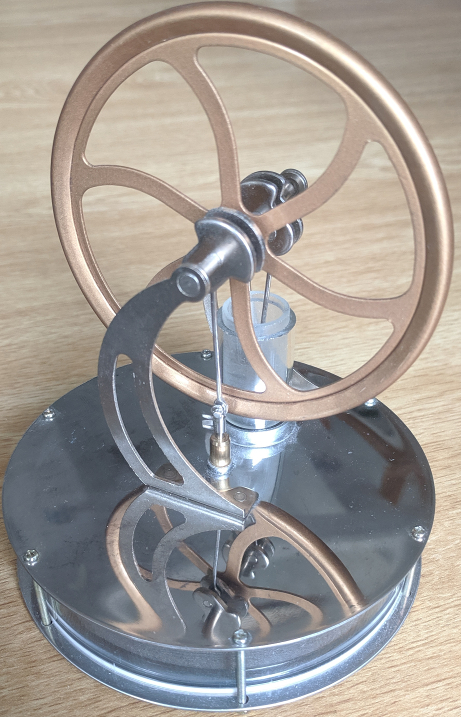
\includegraphics[width=0.3\textwidth]{Figs/introduction/stirling.jpg}
	\caption{The Stirling engine from my desk.}
	\label{fig:stirling}
\end{figure}

\begin{figure}
\centering
\begin{tikzpicture}
[node distance=1.5cm,
    every node/.style={fill=white, font=\sffamily}, align=center]
  % Specification of nodes (position, etc.)
  \node (object)   [activityStarts]              					{Object};
  \node (name)     [activityStarts, right of=object, xshift=4cm] {Name};
  
  \node (A)        [activityStarts, below of=object, yshift=-0.7cm]          {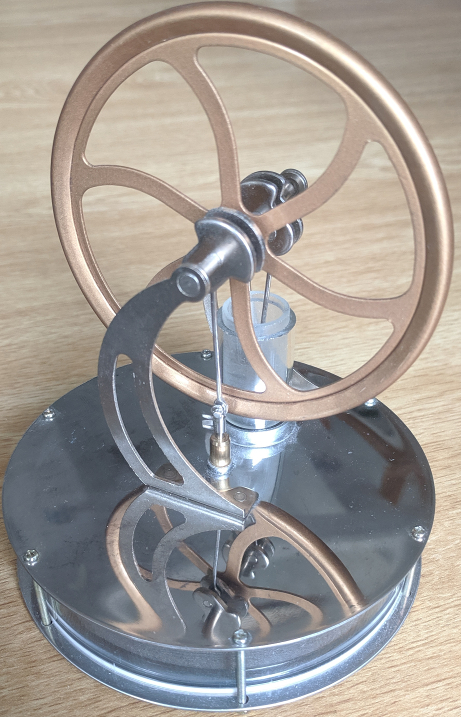
\includegraphics[width=0.96cm,height=1.5cm]{Figs/introduction/stirling.png}};
 \node (stirling) [activityStarts, right of=A, xshift=4cm]  {``Stirling Engine"};       
 
  % Specification of lines between nodes specified above
  % with aditional nodes for description 
  \draw[<->]     (object) -- (name);
  \draw[<->]     (A) -- (stirling);
 
\end{tikzpicture}
\caption{The bi-directional nature of language learning.}
\label{fig:bi_ll}
\end{figure}

The Stirling engine example shows how language learning is a bi-directional process. Not only do you need to learn the name of the object \textit{Stirling Engine} but also that the words ``Stirling Engine'' mean the object \textit{Stirling Engine} as shown in \autoref{fig:bi_ll}. 

Multimodal representation learning allows us to jointly model both the object \textit{Stirling Engine} and the words ``Stirling Engine'', relying on only one assumption: \textbf{Sensory percepts which occur together are related}.

Whilst this may not be true for all sensory percepts it is true enough that co-occurrence of percepts allows us to infer useful information about the relationship between different modalities. For example, smith et al. \cite{smith2008infants} show how infants learn object names based on ``cross-situational statistics'' i.e. how often a word and an object occur together. \autoref{fig:cross_sitch} illustrates this idea.

\begin{figure}[h]
\centering
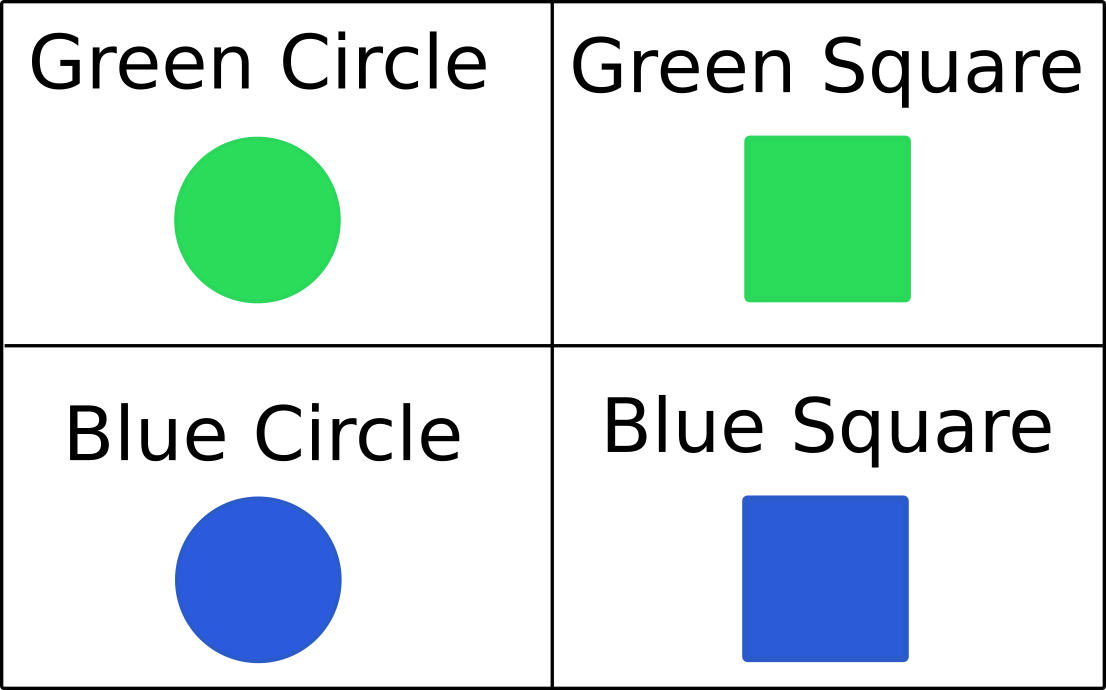
\includegraphics[width=0.5\textwidth]{Figs/introduction/shapes.png}
\caption{Associations among words and objects across multiple ambiguous scenes allow learners to find the proper mapping of words:
\textsc{Circle}, \textsc{Square}, \textsc{Green} and \textsc{Blue} to the shapes and colours: \textit{Circle},  \textit{Square},  \textit{Green} and \textit{Blue}}
\label{fig:cross_sitch}
\end{figure}

Looking at \autoref{fig:cross_sitch} we can see that from a single example, it is not possible to disambiguate which word refers to which part of the image. However, given two examples, it is very easy for an adult human to disambiguate what each word means. As we are given more examples, we can be more and more certain about what we believe the meanings of the words are. 

In the real world, visual perception is much noiser than the images presented in \autoref{fig:cross_sitch} as are the utterances of words. However, by providing more examples, we can overcome the challenges presented by this as shown in \cite{yurovsky2013statistical}. In this thesis I will show how MRL can be applied to this problem and solve it, learning the meanings of different word types, such as object names, colours, sizes and positions as well as the inverse problem, generating these labellings for images of objects. \autoref{fig:mrl_teaser} shows a few examples of MRL solving this problem.

\begin{figure}
\centering

\missingfigure[figwidth=3.5cm]{Placeholder}
\caption{Images generated from labellings of natural images (left) and labellings generated from natural images (right)}
\label{fig:mrl_teaser}
\end{figure}



%----------------------------------------------------------------------------------------







%% Chapter Template
\chapter{A Primer on Artificial Neural Networks} % Main chapter title

\label{Chapter2} % Change X to a consecutive number; for referencing this chapter elsewhere, use \ref{ChapterX}

\lhead{Chapter 2. \emph{A Primer on Artifical Neural Networks}} % Change X to a consecutive number; this is for the header on each page - perhaps a shortened title

%----------------------------------------------------------------------------------------
%	SECTION 1
%----------------------------------------------------------------------------------------
\section{Introduction}
This chapter presents an overview of the mathematical theory behind artificial neural networks and how they learn. It should serve as a quick guide to the techniques used in the experiments in this thesis.

\section{Perceptrons}
\label{sec:percep}
The perceptron is the parent of modern artificial neurons \cite{rosenblatt1958perceptron}.
Perceptrons arranged in layers, referred to as multi-layer perceptrons, are therfore the predecessor of modern artificial neural networks.

\subsection{What is a Perceptron}



\begin{figure}
	\centering
	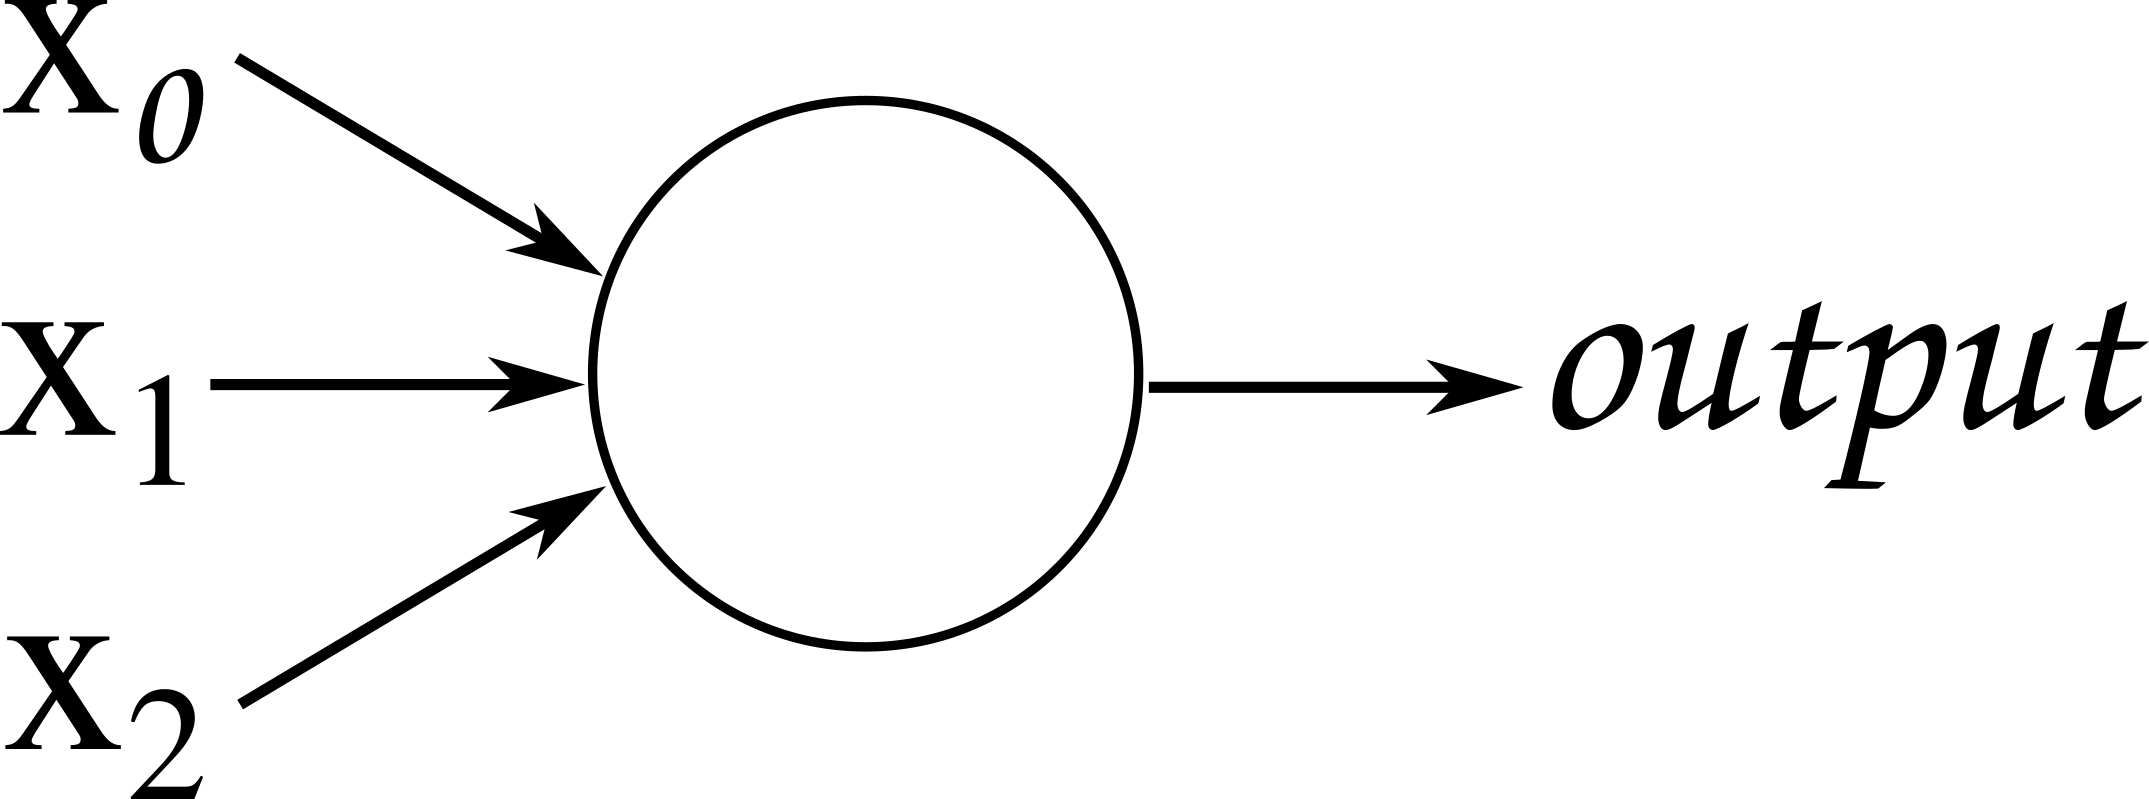
\includegraphics[width=0.4\textwidth]{Figs/intro2dl/perceptron.png}
	
	\caption{A perceptron with three binary inputs, $x_0, x_1, x_2$.}
	\label{fig:perceptron}
\end{figure}

Perceptrons are biologically inspired computation units and are a type of artificial neuron. They take a series of binary inputs, compute a weighted sum and produce a binary output based on the value of this sum as seen in \autoref{fig:perceptron}.


Perceptrons use a binary activation function (\autoref{eqn:percep}).
\begin{equation} \label{eqn:percep}
output = \begin{cases}
0 &\text{if $\sum_{j} w_j x_j + b < 0$}\\
1 &\text{if $\sum_{j} w_j x_j + b \geq 0$}
\end{cases} 
\end{equation}

Where $x_j$ is the jth input, $w_j$ is its associated weight and $b$ is a constant value called the bias, which affects how easy it is for the neuron to activate. The output of the perceptron is caluclated using the formulation shown in \autoref{eqn:percep}.

By adjusting each of the weights we can change the output of the perceptron. For example, if we wanted to use a perceptron to decide whether to have a picnic today we can  select a set of relevant inputs, ``the weather is nice" and ``the pollen count is low".

If it is a sunny day, and the pollen count is high, the input to the perceptron would be $[1,0]$.
 
We will set our weights depending on how important each of the inputs is. No one likes a picnic in the rain, so the weather is important, whilst the pollen count is only important if you suffer from hayfever. We will select a bias of -5 for our perceptron.

For person A, the weights might look like $[7, 0]$ (person A doesn't suffer from hayfever). Therefore the output of the perceptron would be 1 as $(1 \times 7) + (0 \times 0) - 5 = 2$ is greater than 0, so person A will go for a picnic.

Person B owns a large umbrella (so the weather doesn't matter as much) but they do suffer from hayfever, their weights might look like $[4, 7]$. The output of the perceptron would be 0 as  $(1 \times 4) + (0 \times 7) - 5 = -1$ is less than 0. Therefore, person B would wait for a day with a lower pollen count for a picnic.


\subsection{Multi-Layer Perceptron}
In the previous section I demonstrated how a single perceptron can be used to make decisions based on a set of inputs. However, things get much more interesting when we start to link multiple perceptrons together into multi-layer perceptrons (MLP).

\begin{figure}
	\centering
	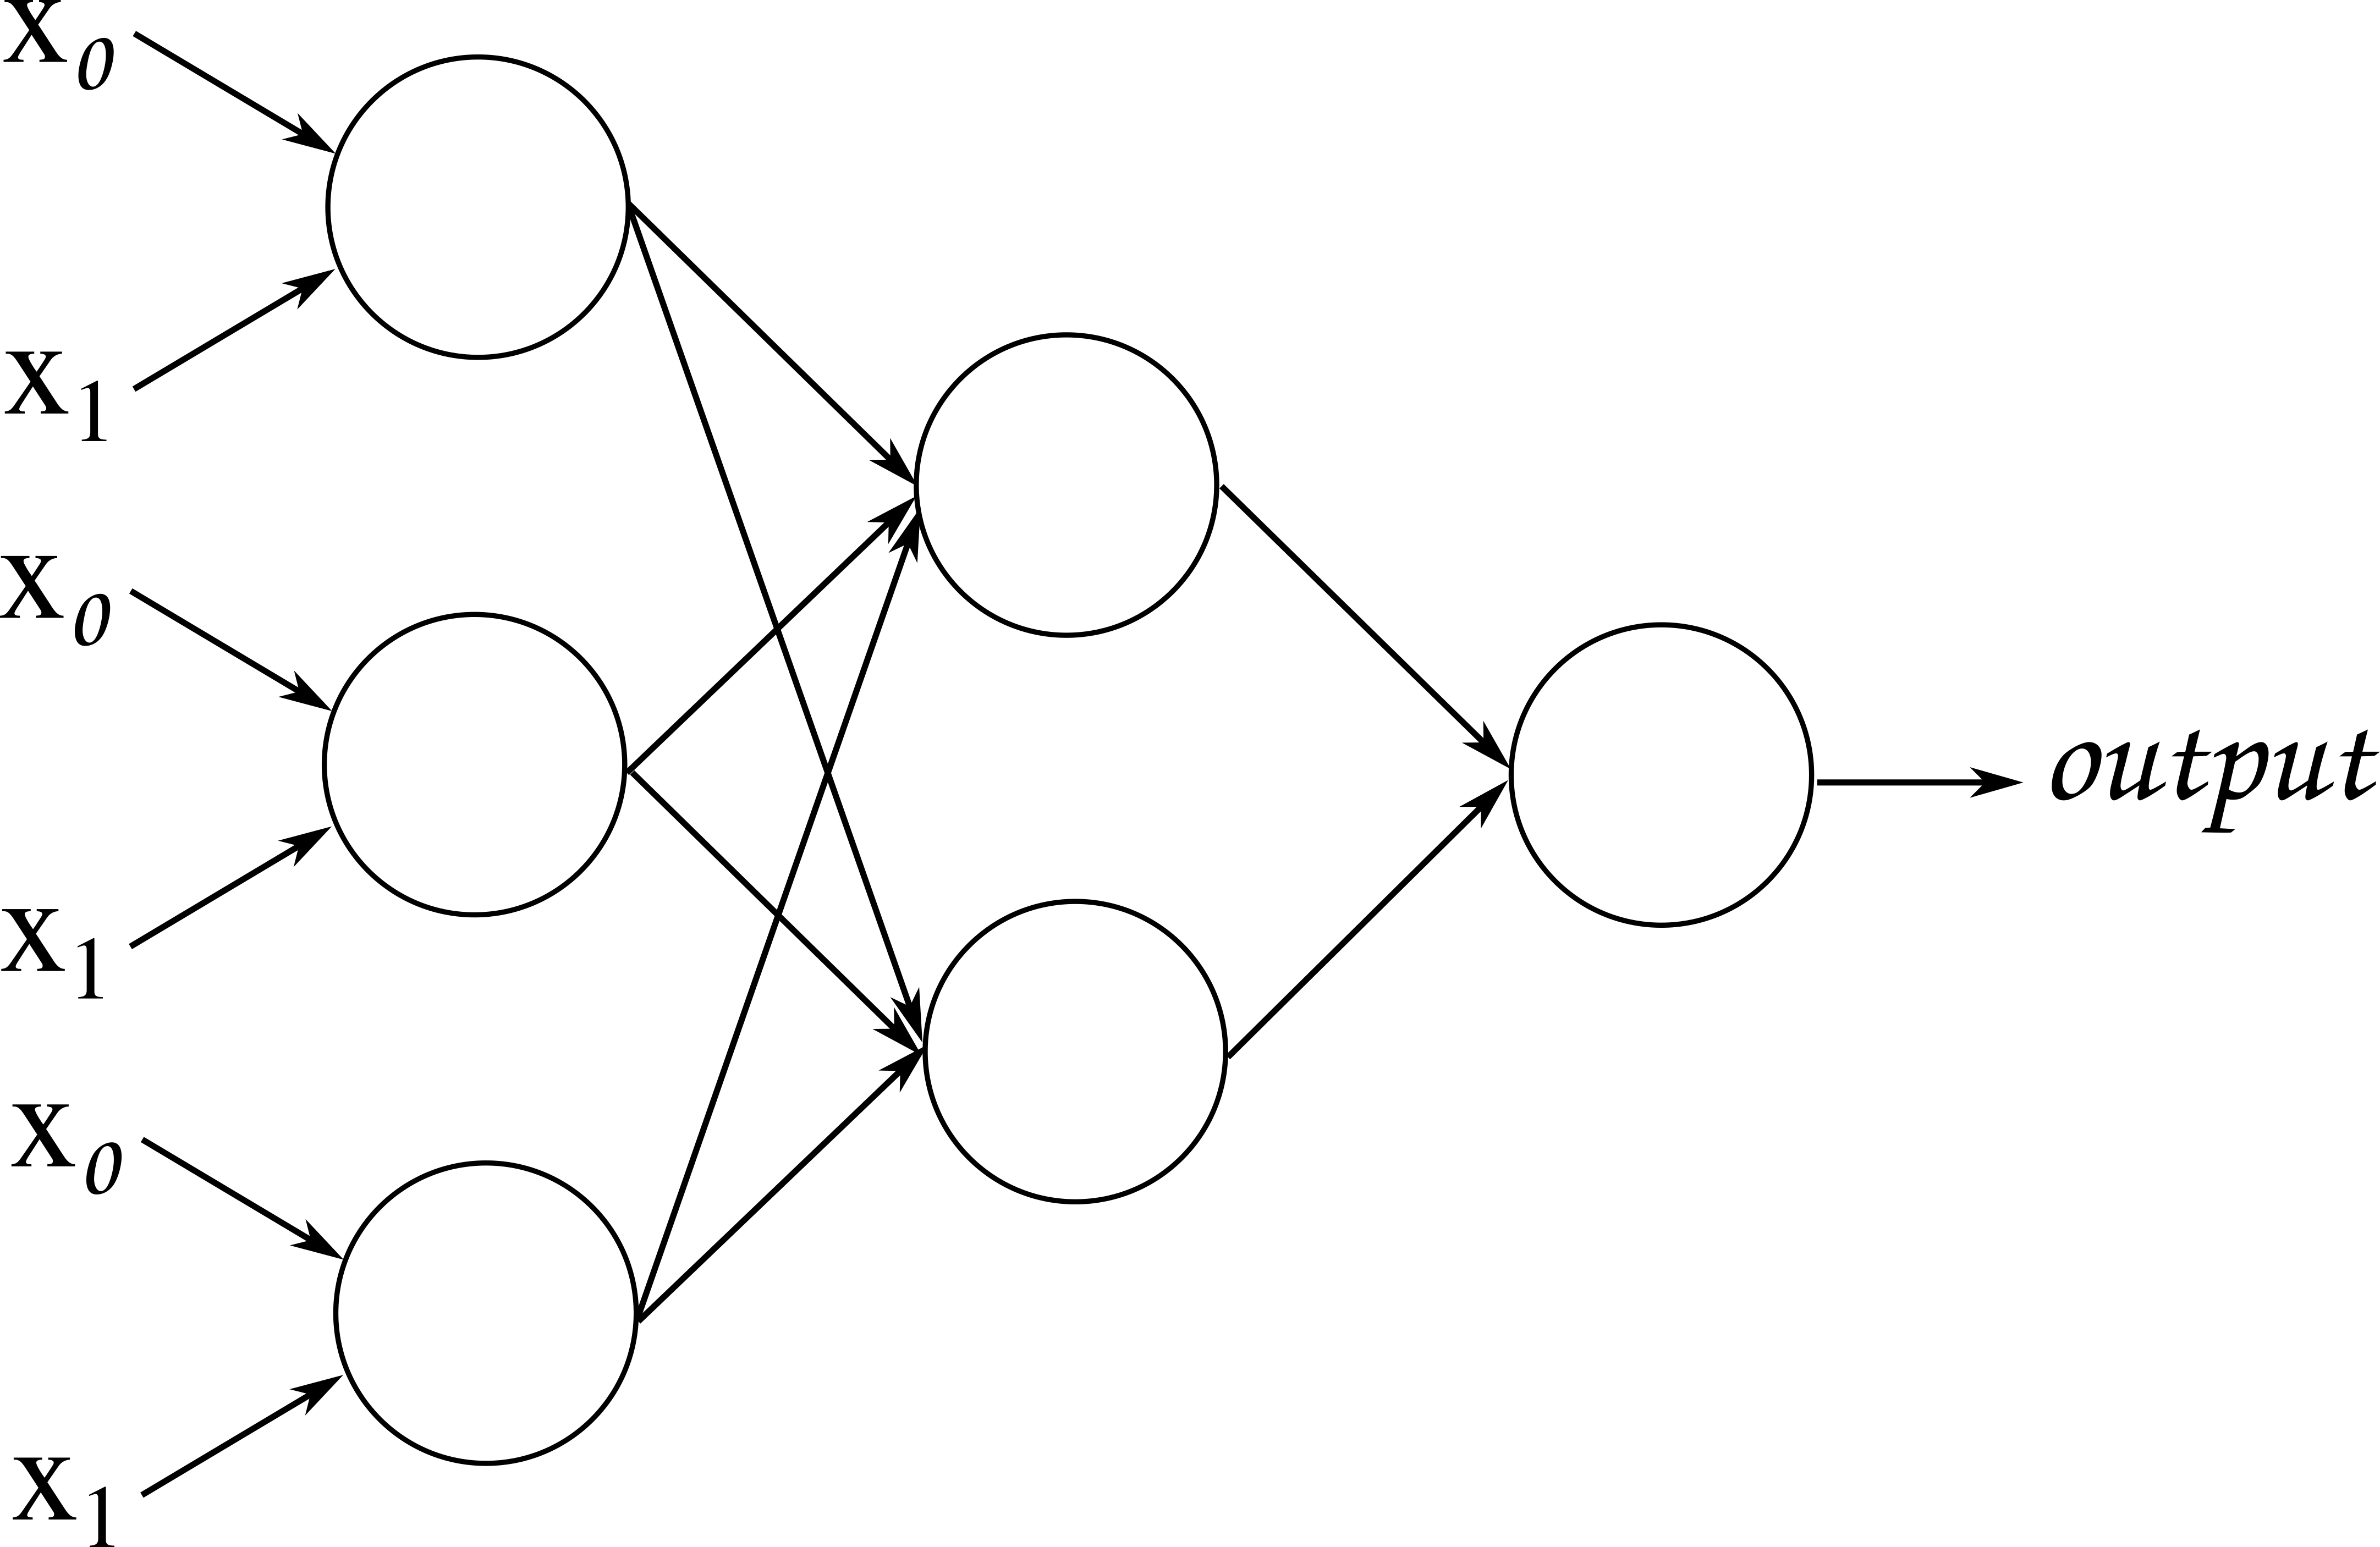
\includegraphics[width=0.4\textwidth]{Figs/intro2dl/mlp.png}
	
	\caption{A multi-layer perceptron consisting of three perceptrons arranged in two layers, with three binary inputs, $x_0, x_1, x_2$.}
	\label{fig:mlp}
\end{figure}

If we take the example from the previous section about deciding to go for a picnic or not, we can use the MLP shown in \autoref{fig:mlp} to consider what happens if person A and B want to go for a picnic together.

Given the previous conditions of a sunny day with a high pollen count, person A wants to go whilst person B does not, as demonstrated by the outputs of their individual perceptrons. Taking these outputs as inputs to the second layer of our MLP, we can see whether the picnic will go ahead.

This time we will set the weights of the second layer based on who shouts the loudest. In this case, person A really wants to go and is very vocal about it. $1 \times 9 + 0 \times 5 - 5 = 4$ so the picnic will go ahead. This resulted in person B developing a headache and sneezing a lot. Clearly we need to find a way to adjust the weights of our MLP so that it makes better decisions in the future.

\section{Activation Functions}

Only being able to handle binary values is a major drawback of the perceptron. An artificial neuron that can handle continuous values is more useful.

This limitation occurs due to the activation function of the perceptron shown in \autoref{eqn:percep}. Visualising the perceptron activation function highlights that changes in the output of the neuron are not proportional to changes in the weights of the neuron as seen in \autoref{fig:activation_percep}. With a few small changes we can make an artifical neuron that accepts continuous values and has a continuous output.

\begin{figure}
\begin{center}
\begin{tikzpicture}

% Us


\begin{axis}[
axis lines=left,
%grid=major,
xtick={-10,0,10},
xticklabels={$-\infty$, 0, $\infty$},
xlabel={Z},
ylabel={Output},
xlabel near ticks,
ylabel near ticks]
\addplot +[blue, thick, mark=none] coordinates{(-10,0) (0,0) (0,1) (10,1)};

\end{axis}

\end{tikzpicture}
\caption{Visualisation of the perceptron activation function. Where z is the activation $\sum_{j} w_j x_j + b$ and the output is activation function defined in \autoref{eqn:percep} }
\label{fig:activation_percep}
\end{center}
\end{figure}

A continuous output is very important as it means that a small change in the weights of a neuron will cause a small change in its output. This makes it much easier to understand how changing the weights affects the output of the network as the change in output becomes proportional to the change in weights as shown in \autoref{eqn:proport}.

\begin{equation} \label{eqn:proport}
	\delta Output \propto \delta W	
\end{equation}  


\subsection{Sigmoid Neurons}

The sigmoid neuron uses the sigmoid function, shown in \autoref{eqn:sig} as its activation function. 

\begin{equation} \label{eqn:sig}
\sigma(z) = \frac{1}{1 + e^{-z}}
\end{equation}

$z$ is the sum of the weights multiplied by their respective inputs as seen in  \autoref{eqn:z_act}.

\begin{equation} \label{eqn:z_act}
z = \sum_{j} w_j x_j + b
\end{equation}

As we can see in \autoref{fig:activation_sigmoid}, as $z$ changes, there is a proportional change in the output $\sigma(z)$, unlike in \autoref{fig:activation_percep} where the output only changes when $z$ crosses the y-axis.

\begin{figure}
\begin{center}
\begin{tikzpicture}



\begin{axis}[
axis lines=left,
xtick={-10,0,10},
xticklabels={$-\infty$, 0, $\infty$},
xlabel={z},
ylabel={$\sigma$(z)},
xlabel near ticks,
ylabel near ticks,
%grid=major
]
\addplot[blue, thick, smooth, samples=1000, domain=-10:10]{1 / (1 + e^-x)};

\end{axis}
    

\end{tikzpicture}
\caption{Visualisation of the Sigmoid activation function. Where z is the activation $\sum_{j} w_j x_j + b$ and $\sigma$(z) is activation function defined in \autoref{eqn:sig} }
\label{fig:activation_sigmoid}
\end{center}
\end{figure}

Now that we have an activation function that can produce continuous values, we can consider a much more diverse range of data to train our neural networks with. So instead of just making yes or no decisions we can look at, for example, the colours of pixels and decide if there is a cat in the image or given today's weather, predict if it will rain tomorrow.

\subsubsection{Other activation functions}
There are two other important and commonly used activation functions, though many others exist. These are, the hyperbolic tangent (Tanh) shown in \autoref{fig:activation_tanh} and rectified linear unit (Relu)  shown in \autoref{fig:activation_relu}.

\begin{figure}
\begin{center}
\begin{tikzpicture}
\begin{axis}[
axis lines=left,
xtick={-10,0,10},
xticklabels={$-\infty$, 0, $\infty$},
xlabel={z},
ylabel={$\sigma$(z)},
xlabel near ticks,
ylabel near ticks,
]
\addplot[blue, thick, smooth, samples=100, domain=-10:10]{tanh(x)};

\end{axis}
    

\end{tikzpicture}
\caption{Visualisation of the hyperbolic tangent activation function. Where z is the activation $\sum_{j} w_j x_j + b$ and $\sigma$(z) is the Hyperbolic Tangent Function applied to z.}
\label{fig:activation_tanh}
\end{center}
\end{figure}

The Tanh function looks similar to the sigmoid function, however it has an output between negative one and one, where the sigmoid goes from zero to one. This is useful when negative values are important to what the network is learning.

\begin{figure}
\begin{center}
\begin{tikzpicture}
\begin{axis}[
axis lines=left,
xtick={-10,0,10},
xticklabels={$-\infty$, 0, $\infty$},
xlabel={z},
ylabel={$\sigma$(z)},
xlabel near ticks,
ylabel near ticks,
]
\addplot[blue, thick, smooth, samples=1000, domain=0:10]{x};
\addplot[blue, thick, smooth, samples=1000, domain=-10:0]{0};

\end{axis}
    

\end{tikzpicture}
\caption{Visualisation of the rectified linear unit activation function.Where z is the activation $\sum_{j} w_j x_j + b$ and $\sigma$(z) is the Relu activation function applied to z.}
\label{fig:activation_relu}
\end{center}
\end{figure}

The Relu was created to address an issue known as vanishing gradients. This is to do with how neural networks are trained, as expalined in the next section. Briefly, as training depends on error gradients, having a linear activation function means that deeper networks \endnote{Deeper networks are beneficial as they can make more complex decisions by layering more and more simple decsions as shown in the MLP example in \autoref{sec:percep}} can be trained as non-linear functions (like the Sigmoid or Tanh) will have reduced gradient magnitude when they are differentiated to backpropogate the error through the network. If that doesn't make sense yet, don't worry, it will become clear shortly.

\section{Learning Algorithms}
In \autoref{sec:percep} we saw how simple computation units can make simple decisions and how these can be chained together to make more complex decisions. However, sometimes the decisions we make are wrong and we need to learn from our mistakes.

In general, perceptrons (and their more modern successors) will have their initial weights set randomly, unlike in our example where I chose them. 

Randomly setting weights is useful in practice as we will usually have large numbers of inputs, weights, layers and artifical neurons, so setting each by hand would be intractable. Also, if we knew what weights to set, we wouldn't need a neural network or a learning algorithm to solve our problem as we would likely have a more efficient mathematical description of the problem.

With random weights our networks will make a lot of wrong decisions! However if we have a smart way of adjusting our weights we can make our neural networks get better at making decisions over time. This improvement is what I am referring to when I say ``machine learning''.

\subsection{Types of Training}
There are many ways to train neural networks: supervised, unsupervised, reinforcement or 
adversarial learning (to name a few). The experiments in this thesis will focus on supervised and unsupervised learning. %However, here is a brief description of the more prominant methods.


\textbf{Supervised learning} - an external system is used to provide ground truth values for the desired output of the network. An example would be classification using standardised datasets like MNIST handwritten digits \cite{lecun1998mnist}.


\textbf{Unsupervised learning} - no external system provides ground truth values, instead these are inferred directly from the data. Autoencoders (discussed in great detail in later chapters) are a good example of this.  

%\todo[inline]{finish this}
%\textbf{Reinforcement learning} - an external system provides a score which estimates the value of an action (think about getting points in a video-game). Training a dog by giving it treats when it performs a trick is reinforcement learning. We reinforce the desired behaviour by rpoviding a reward.

%\textbf{Adversarial learning} - two networks are trained in tandom, a generator and a descriminator. The


\subsection{Cost functions: How wrong am I?}
In order for our neural networks to learn, they need feedback as to how wrong they are. This is done using a cost function, a formula which gives a measure of how good or bad our network is at a particular task.

Depending on the particular method we use to train our networks, the cost function may be given a different name. For example in reinforcement learning, the cost function is typically called a value function. However, they all serve the same purpose, which is to provide feedback as to how well our network is doing at the task it has been assigned. Therefore, to avoid jargon I will refer to this as a \textit{cost function} throughout this thesis and the measure it returns as the \textit{error}.

The cost function can take on many forms, in supervised and unsupervised training alike. Here are a few of the more commonly used ones and an explanation of each.

\subsubsection{Mean Squared Error}
Mean squared error (MSE) measures the average difference between points as shown in \autoref{eqn:mse}.

\begin{equation} \label{eqn:mse}
C = \frac{1}{n}\sum_{i=0}^{n} (Y_i - \hat{Y_i})^2
\end{equation}

When used as a loss function, MSE gives a measure of how bad our estimate $\hat{Y_i}$ is of our true value $Y_i$ on average for for all $n$ training samples in a given dataset. A perfect model would have an MSE of 0 as $\hat{Y_i}$ would be equal to $Y_i$ for all values of $i$.

In general, $Y_i$ and $\hat{Y_i}$ can be of arbitrary size and shape (as long as they match each other). That is, they can be scalers, vectors or matricies.

\subsubsection{Cross-Entropy}
Cross-entropy measures the error between two probability distributions $P$ and $Q$ using the formula shown in \autoref{eqn:xntrpy}. $P$ is the true probability distribution which we are trying to model with our predicted probability distribution $Q$.

\begin{equation} \label{eqn:xntrpy}
C = -\sum_{i=0}^{n}P(i) log(Q(i))
\end{equation}

When using cross-entropy as a loss function, we can view the output of our neural network as a probability distribution. For example, in a multiclass classification problem with $k$ classes, each of the $k$ outputs of the network tells us the probability that the network believes an input to belong to class $k$.


For example, given a dataset containing images of animals: cats, dogs, horses and snakes. A single image containing a cat would be labelled $[1, 0, 0, 0]$. This tells us the exact probability distribution of the image, $P$ i.e. the image certainly contains a cat and does not contain any other animals.

Now as our network trains, it may give a prediction of $[0.5, 0.3, 0.15, 0.05]$, this is our predicted probability distribution $Q$.

Calculating our cross-entropy we get:
$C = -(1 log(0.5) + 0 log(0.3) + 0 log(0.15) + 0 log(0.05) = 0.301_{3s.f.})$


If we then do some training using gradient descent our network might then predict $[0.8, 0.2, 0, 0]$ giving a cross-entropy of $0.0969_{3s.f.}$. Clearly this represents an improvement, as the error is closer to zero and our prediction is better. The network believes with 80\% certainty that the images is of a cat. 


\subsubsection{Kullback-Leibler Divergence}

Another method for defining the difference between two distributions is the Kullback-Leibler Divergence (KLD).

KLD is a non-symetric distance measure between two distributions, $P$ and $Q$. As it is non-symetric $D_{KL}(P||Q) \neq D_{KL}(Q||P)$ unless $P = Q$.

\begin{equation} \label{eqn:kld}
D_{KL} = -\int_{i=0}^{n}{P(i)Log(\frac{Q(i)}{P(i)}})
\end{equation}

KLD is useful in machine learning when we wish to calculate how different a predicted distribution is from a desired distribution. Most commonly, we will want $P$ to be a Gaussian distribution, though which distribution is chosen will depend on the specific problem. We will then use the KLD as a constraint to force our networks to make predictions which follow as closely as possible to this desired distribution, i.e. we will minimse $D_{KL}(P||Q)$.

Typically KLD is not used as a cost function on its own, but is used to constrain the output of a single layer of a network (usually not the output) whilst also minimising another cost function.

The best example of this is a Variational AutoEncoder (VAE), which will be discussed later.


\subsection{Gradient Descent}
Now that we have a method for determining how well our neural network performs at a task, we can observe how this changes as the weights of the network are changed.

\pgfplotsset{%
  colormap={whitered}{color(0cm)=(white);
  color(1cm)=(orange!75!red)}
}

\begin{figure}
\begin{center}
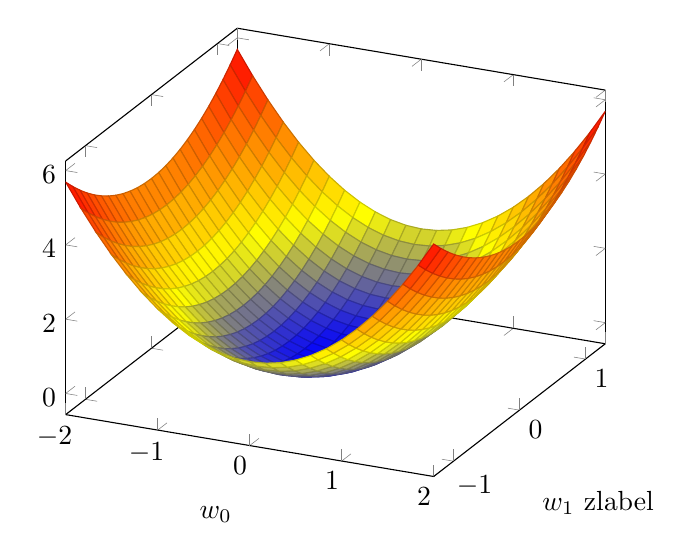
\begin{tikzpicture}
 
  \begin{axis}[
  xlabel = $w_0$,
  ylabel = $w_1$
  zlabel = $C$
  ]
   
    \addplot3[
	surf,
	domain=-2:2,
	domain y=-1.3:1.3,
] 
	{x^2+y^2};

    
  \end{axis}
\end{tikzpicture}
\caption{The cost landscape of a bivariate function. Where $w_0$ and $w_1$ are the weights of a neural network and $C$ is its error.}
\label{fig:costscape}
\end{center}
\end{figure}

To make things simple, lets assume our network only has two weights, though the following derivation generalises to any number of weights. This could give us a cost landscape like that shown in \autoref{fig:costscape}. Our aim is to minimise the cost as the cost is a measure of how wrong our network is.

In more definite terms we wish to minimise \autoref{eqn:cost_bivar}, where $Y_i$ is the desired output value for input $i$ and $z$ is as defined in \autoref{eqn:z_act}.

\begin{equation} \label{eqn:cost_bivar}
C(w_0, w_1) = \frac{1}{n}\sum_{i=0}^{n} (Y_i - \sigma(z_i))^2
\end{equation}

This is the mean squared error rewritten slightly to highlight the dependence on the weights of the network.

If we make a small change to either of the weights $w_0$ and $w_1$ we will get a small change in the cost, $C$ as seen in \autoref{eqn:delta_C}.

\begin{equation} \label{eqn:delta_C}
\Delta C \approx \frac{\delta C}{\delta w_0} \Delta w_0 + \frac{\delta C}{\delta w_1} \Delta w_1
\end{equation}

We want to minimise C so we want $\Delta C$ to be negative. To make $\Delta C$ negative we will need to first denote that the gradient of $C$, $\nabla C$. 

\begin{equation} \label{eqn:nabla_c}
\nabla C \equiv (\frac{\delta C}{\delta w_0}, \frac{\delta C}{\delta w_1})^T
\end{equation}

In \autoref{eqn:nabla_c} we can see that the gradient of $C$ is equivalent to the partial derivatives of $C$ with repect to the weights of the network. For simplicity we will collect the changes in weights into a single vector $\Delta w \equiv (\Delta w_0, \Delta w_1)^T$.

By substituing this into \autoref{eqn:delta_C} we get \autoref{eqn:delta_c_sub}.

\begin{equation} \label{eqn:delta_c_sub}
\Delta C \approx \nabla C \cdot \Delta w 
\end{equation}

Looking at \autoref{eqn:delta_c_sub}, we can see that to make $\Delta C$ negative we can set $\Delta w$ as in \autoref{eqn:delta_w_eta}, where $\eta$ is a small positive constant called the learning rate.

\begin{equation} \label{eqn:delta_w_eta}
\Delta w = -\eta \nabla C
\end{equation}

By substituting \autoref{eqn:delta_w_eta} into \autoref{eqn:delta_c_sub} we can see that $ \Delta C = - \eta \abs{\nabla C}^2$ and because $\abs{\nabla C}^2 \geq 0$ this guarantees that $C$ will always decrease if the weights are changed in accordance to \autoref{eqn:delta_w_eta}.

By iteratively making changes to the weights according to \autoref{eqn:delta_w_eta}, we will eventually reach the minima of $C$ so long as we select an appropriate learning rate \endnote{Learning rate is discussed in more detail in \autoref{sec:lr_sch}}. 

\subsection{Backpropagation}
With a gradient descent providing a method for adjusting  weights, we now only need one more ingredient to be able to train our neural networks. Whilst our cost function tells us about the error of our network at its output, we need a method to calculate the error for any neuron in any layer - this is exactly what backpropagation does. 

A full explanation of the backpropogastion algorithm is available in \autoref{appendix:app3}. However, understanding this backpropogation is not necessary to understand the contribution of this thesis.


\subsection{Extensions and Improvements}
There are many extensions to simple gradient descent based learning, here are a few to be aware of.
\subsubsection{Learning Rate Schedule}
\label{sec:lr_sch}
Depending on how far we are from the global error minima, we may wish to change the value of the learning rate $\eta$. Recall from \autoref{eqn:delta_w_eta} $\Delta w = -\eta \nabla C$, that the learning rate determines how big of a step we take, following the gradient of the error, each time we update the weights of our neural network.

If we are far from the minimum point for the cost with respect to the weights, we may wish to take larger steps, so that we can more quickly reduce the total cost. However, as we get closer we want to ensure that we do not step over the minimum.

\begin{figure}
\begin{center}
\begin{tikzpicture}
\begin{axis}[
axis lines=left,
xtick={-10,0,10},
xticklabels={},
xlabel={$\Delta w$},
ylabel={$C$},
yticklabels={},
xlabel near ticks,
ylabel near ticks]
\addplot[black, thick, smooth, samples=1000, domain=-10:10]{x^2};
%\draw [blue](0,100) ++(90 : 1 ) arc ( 90:81.87:50 );
\node [blue] at (2,98)  (a) {\textbullet};
\node [blue] at (20,64) (b) {\textbullet};
\node [blue] at (40,36) (c) {\textbullet};
\node [blue] at (60,16) (d) {\textbullet};
\node [blue] at (80,4)  (e) {\textbullet};
\node [blue] at (100,0) (f) {\textbullet};

\draw[blue, ->](a) to [bend left] (b);
\draw[blue, ->](b) to [bend left] (c);
\draw[blue, ->](c) to [bend left] (d);
\draw[blue, ->](d) to [bend left] (e);
\draw[blue, ->](e) to [bend left] (f);


\node [red] at (198,98)  (g) {\textbullet};
\node [red] at (180,64) (h) {\textbullet};
\node [red] at (153,28) (i) {\textbullet};
\node [red] at (90,1) (j) {\textbullet};
%\node [red] at (60,16)  (k) {\textbullet};
%\node [red] at (80,4) (l) {x};


\draw[red, ->](g) to [bend right] (h);
\draw[red, ->](h) to [bend right] (i);
\draw[red, ->](i) to [bend right] (j);
%\draw[red, ->](j) to [bend right] (k);


\end{axis}
    

\end{tikzpicture}
\caption{Visualisation of error minimisation in two dimensions for different learning rate schedules. Blue: decreaseing learning rate, Red: large fixed learning rate. Where $\delta w$ is the change of weights of a neural network and and $C$ is its error.}
\label{fig:lr_schedule}
\end{center}
\end{figure}

\autoref{fig:lr_schedule} shows how changing the learning rate schedule can affect how the gradient descent optimiser navigates the cost landscape. As more training occurs, reducing the learning rate allows us to reach the error minimum (blue arrows). Selecting a large learning rate not changing it might lead to never reaching the error minimum (red arrows). Whilst at first, we make rapid progress towards the minimum, at some point we cross over it and will be unable to approach any closer without taking smaller steps.

This demonstrates nicely why we either select a small learning rate or make use of a learning rate scheduler.
Learning rate schedulers can speed up convergence by allowing large steps to be taken when we are far from the cost minimum with respect to the weights, covering a large distance in a few updates and then slowing down to take smaller steps as we get closer. 

This begs the question of: how do we know when to change the learning rate? In  practice there are many ways we can achieve this, however these broadly fit into two categories: mathematical and heuristic.

There are many algorithms for calculating how to set the learning rate for example, Adam \cite{kingma2014adam} and ADADelta \cite{zeiler2012adadelta}. They are both popular as they are both first order methods, meaning that expensive, slow calculations of second order derivatives do not need to be made.
Senior et al.\cite{senior2013empirical} provide an extensive testing of different learning rate schedulers. 

Second order methods are desirable in that the second derivative of the cost provides information about how the cost gradient is changing. \autoref{fig:2ndordr} shows how the cost and its first and second derivatives change with respect to the weights. In region (A), where the cost (black line) is far from the minima the first derivative (blue) changes rapidly, causing the second derivative (red) to have a large magnitude. In region (B), the cost is closer to the minima, and thus the change in cost is lower so the steepness of the first derivative (blue) is lower as is the magnitude of the second derivative (red). At the minima, the second derivative is exactly zero, so we know we have reached the minima if the second derivative equals zero.

Second order methods have the major draw back of being very slow to calculate. Thus it is more efficient to make use of first order estimates than the exact information provided by second order methods. Many more weight updates can be carried out using first order methods than can be done using second order methods in a given time frame. So whilst second order methods should require less total weight updates to minimise the cost, the first order methods will reach the minimum faster as the weight updates will occur much more quickly in the first order case.


\begin{figure}
\begin{center}
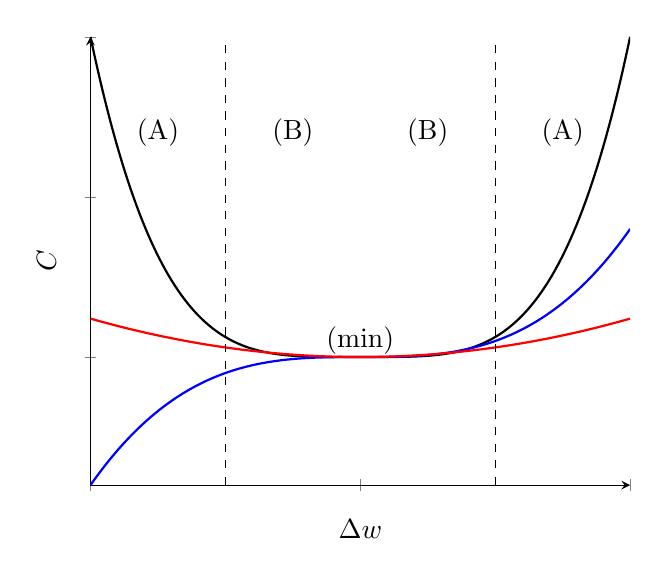
\begin{tikzpicture}
\begin{axis}[
axis lines=left,
xtick={-10,0,10},
xticklabels={},
xlabel={$\Delta w$},
ylabel={$C$},
yticklabels={},
xlabel near ticks,
ylabel near ticks,
scaled y ticks = false]
\addplot[black, thick, smooth, samples=1000, domain=-10:10]{x^4};
\addplot[blue, thick, smooth, samples=1000, domain=-10:10]{4*x^3};
\addplot[red, thick, smooth, samples=1000, domain=-10:10]{12*x^2};

\addplot [black, thin, dashed] coordinates {(-5, -4000) (-5, 10000)};
\addplot [black, thin, dashed] coordinates {(5, -4000) (5, 10000)};

\node[] at (axis cs:7.5,7000) {(A)};
\node[] at (axis cs:-7.5,7000) {(A)};
\node[] at (axis cs:2.5,7000)  {(B)};
\node[] at (axis cs:-2.5,7000) {(B)};
\node[] at (axis cs:0,500) {(min)};



\end{axis}
    

\end{tikzpicture}
\caption{Visualisation of the cost (black), its first derivative (blue) and second derivative (red). Where $\delta w$ is the change of weights of a neural network and and $C$ is its error.}
\label{fig:2ndordr}
\end{center}
\end{figure}

Heuristic methods provide a very simple method for adjusting the learning rate. A commonly used one is to simply gradually reduce the learning rate by a small amount each epoch. This has the advantage of requiring almost no computational overhead and being easily understood. When training starts, we expect performance to be poor, so improvements can be made rapidly. As training progresses, we expect that improvements will be slower as we are approaching the minimum cost.

\section{Convolutional Neural Networks}
One draw back of dense neural networks, like MLPs is that they do not leverage spatial information in the input data. This means that whether two pieces of information occur next to each other, is irrelevant to the neural network. Obviously, this information is important and useful, so how can a neural network use it?

Consider two very different problems: image classification and speech recognition. In image classification, not only are the values of pixels important but also, the values of pixels surrounding them. For example, we know that \autoref{fig:cat} is a picture of a cat, not just because there are grey pixels on a white background, but because the grey pixels are collected into a cat-like shape. We are unable to recognise the right hand image despite have the same pixels as the left image as spatial cues have been removed.

\begin{figure}
	\centering
	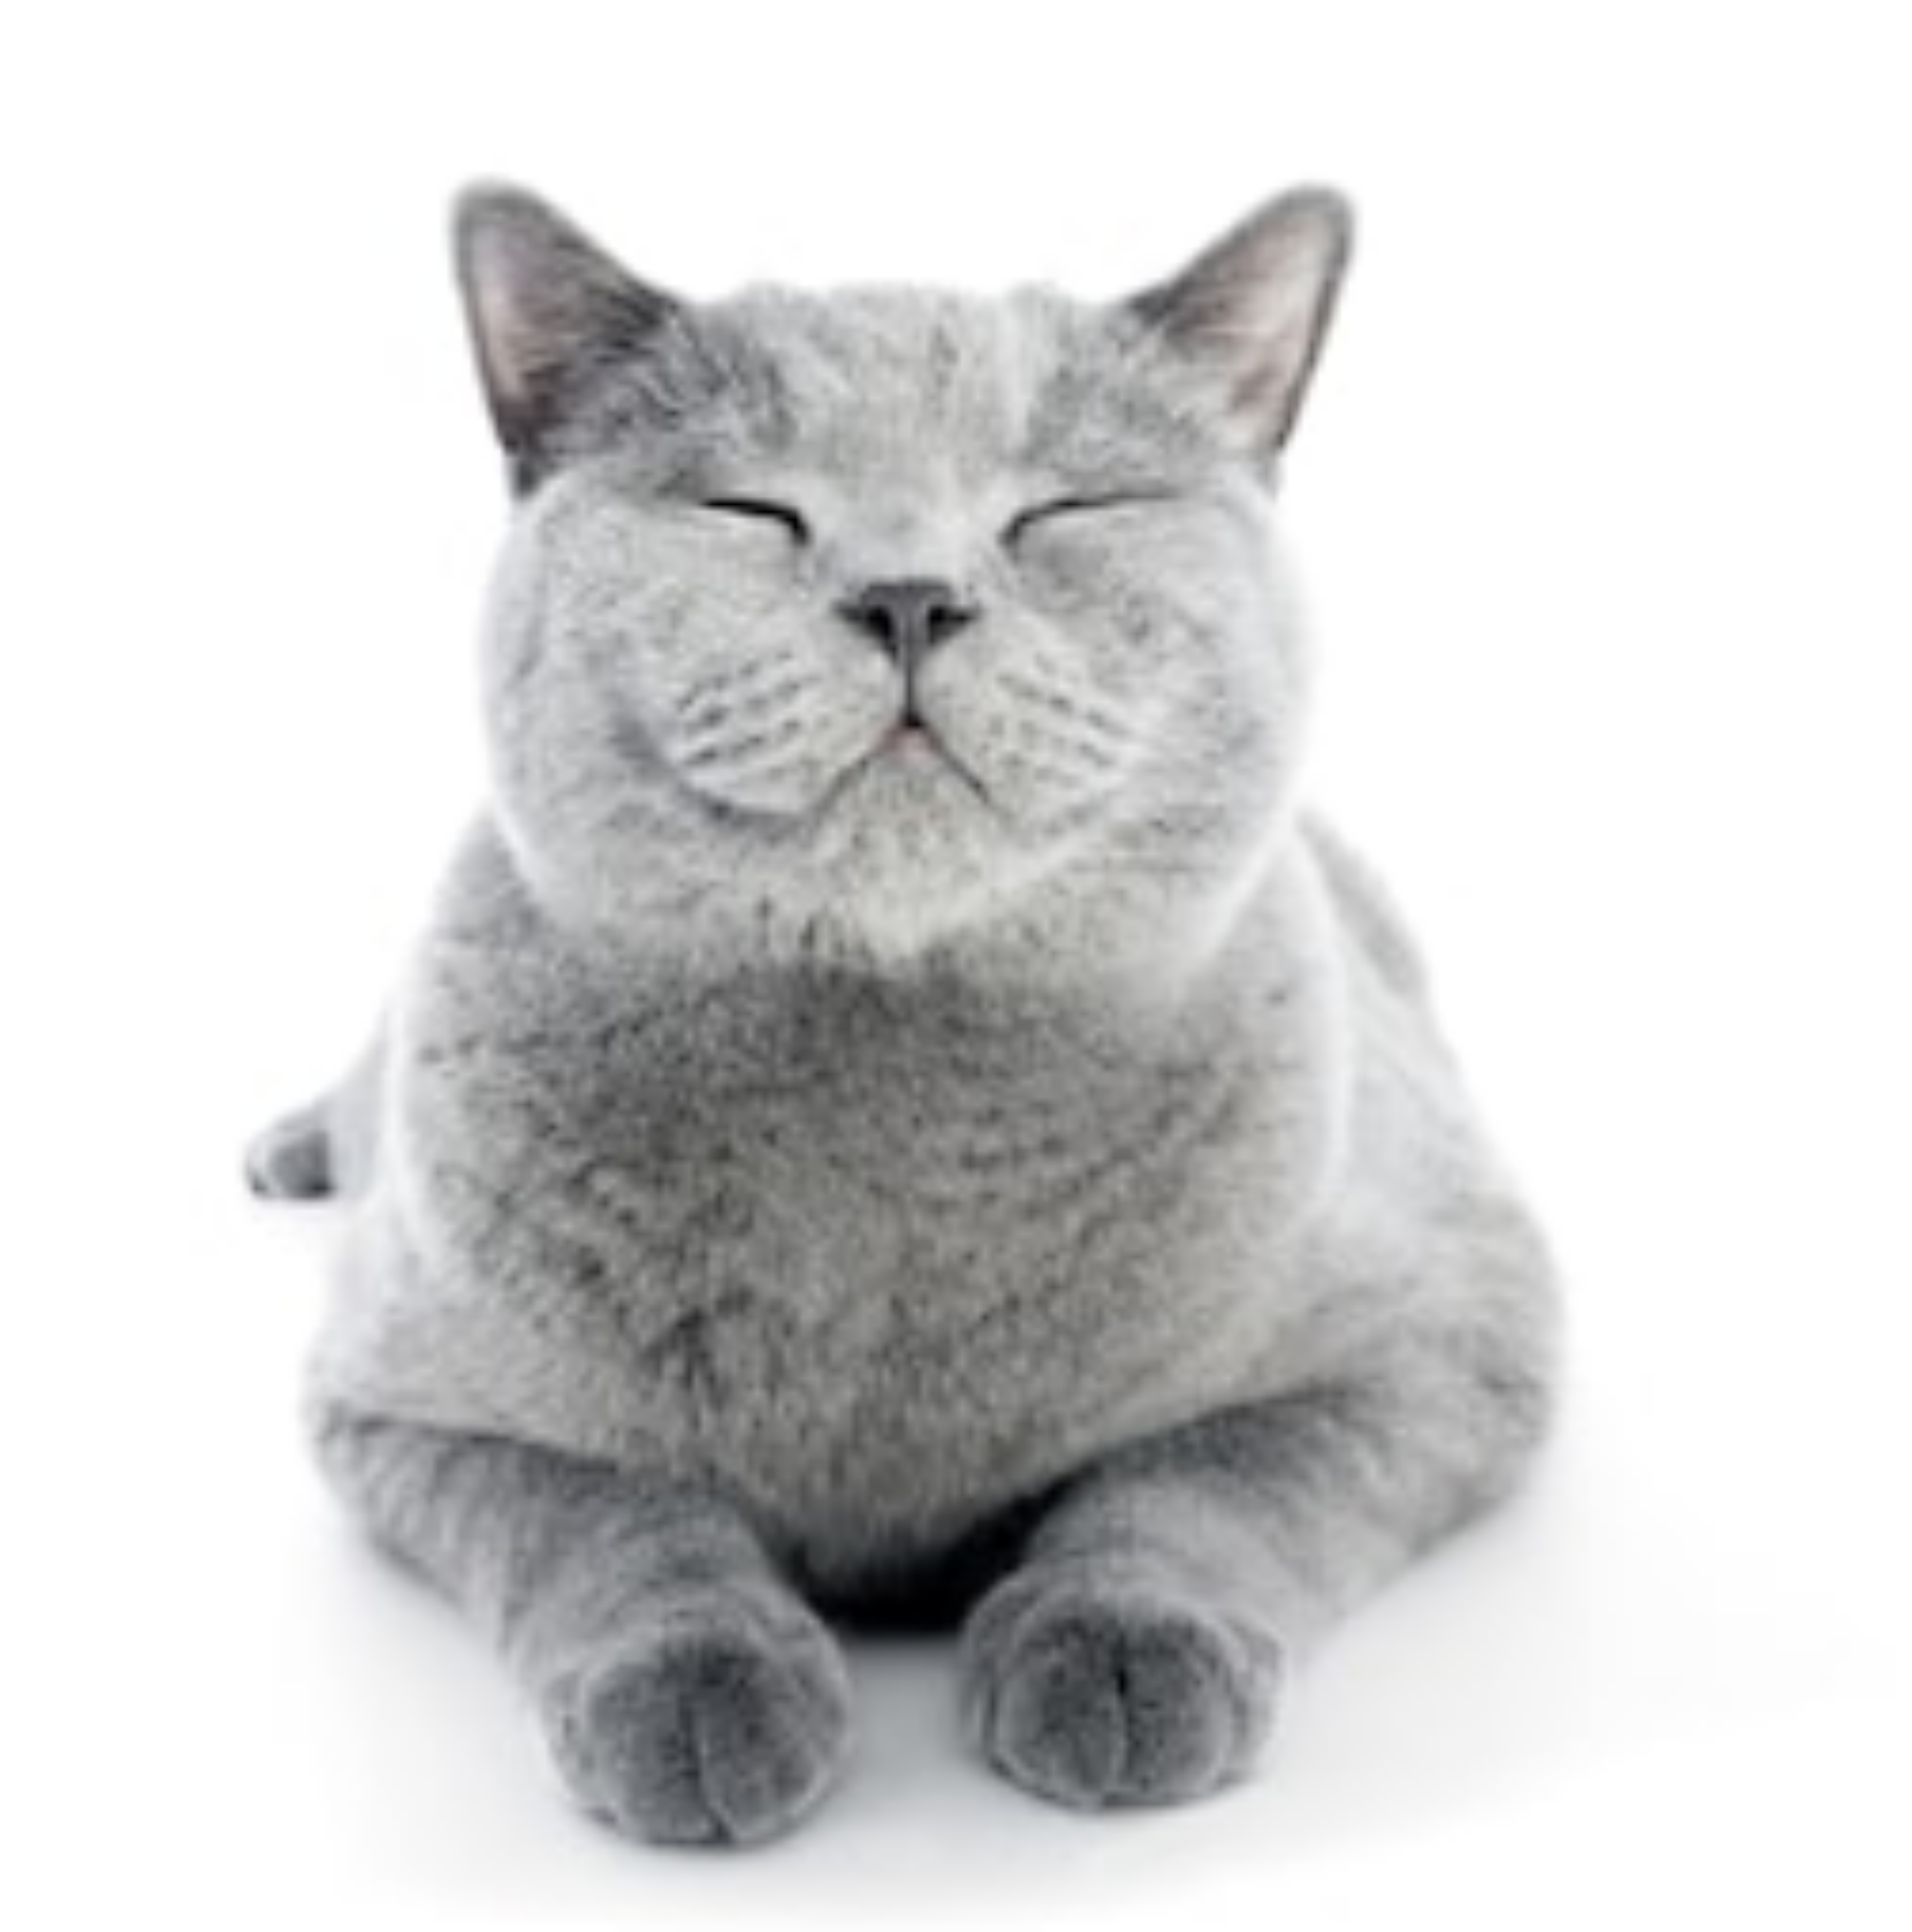
\includegraphics[width=0.33\textwidth]{Figs/intro2dl/cat.png}
	\includegraphics[width=0.33\textwidth]{Figs/intro2dl/catScrambled.png}
	
	\caption{A british short-hair cat (left) and the same image, with its pixels scrambled (right).}
	\label{fig:cat}
\end{figure}

Similarly, in speech recognition, the order in which sound samples are heard is very important. If we hear a word backwards, we won't recognise it as being that word and if we re arrange the order of the samples, it becomes even more difficult to recognise.

Dense neural networks don't care about spatial information because each input is connected to every neuron in the input layer, effectively treating every pixel as if they are no closer, or further away from any other pixel or removing information about when each sample of sound occured.

In order to levarge spatial information we can make use of convolutional neural networks (ConvNet).

\subsection{What is Convolution?}
In ConvNets, convolution is a mathematical operation which adds a data element to its neighbours, weighted by a kernel. For example, given a 3x3 kernel, and an image as the input data each pixel $P_{out}(i,j)$ in the output of the convolution will be the sum of the pixels $P_{in}(i-s, j-t)$ in the input  multiplied by its respective kernel weight $k(s,t)$ as seen in \autoref{eqn:convolution} \cite{dumoulin2016guide}.

\begin{equation} \label{eqn:convolution}
P_{in}*k = \sum_{s=-a}^{a}\sum_{t=-b}^{b} P_{in}(i-s, j-t) \circ k(s,t)
\end{equation}

\begin{figure}
	\centering	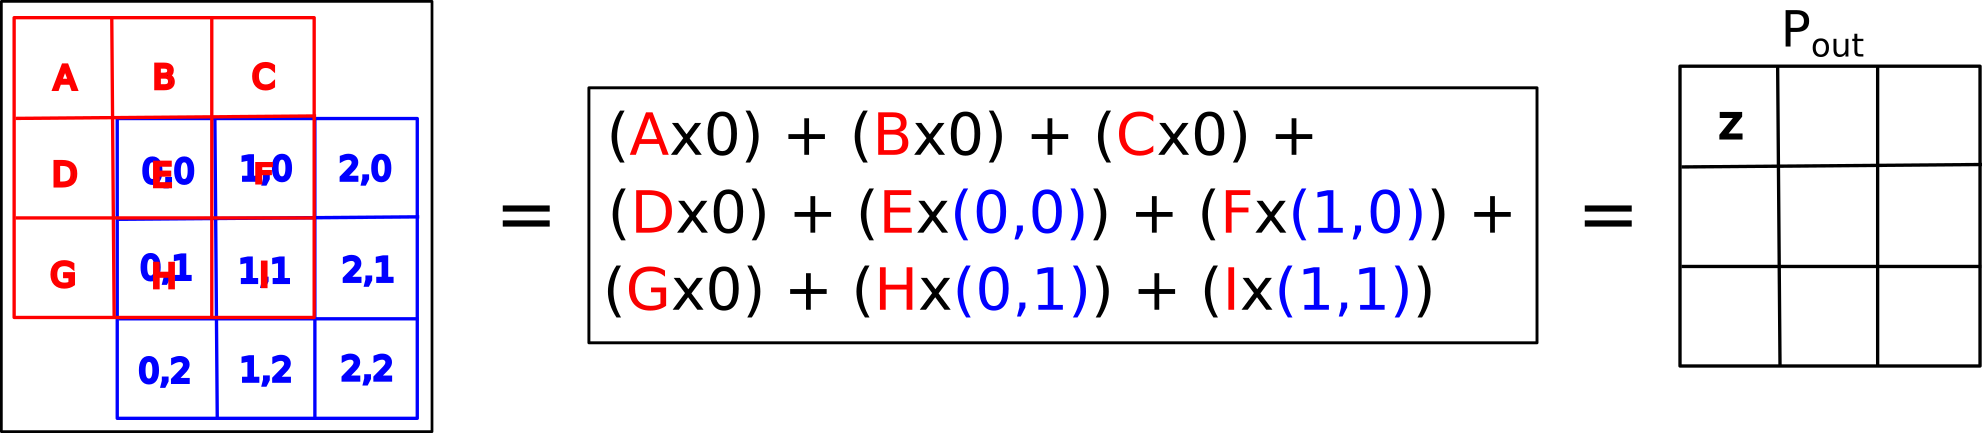
\includegraphics[width=0.75\textwidth]{Figs/intro2dl/convolutionSingleStep.png}
	\caption{A single step of computing a convolution }
	\label{fig:oneStepConv}
\end{figure}

Consider the case where $P_{in}$ is a 3x3 array and $k$ is a 3x3 kernel. The convolution, $P_{in} * k$ would unfold as shown in \autoref{fig:oneStepConv}. $P_{out}$ will take values dependant on the sum of the elements of $P_{in}$ multiplied by the weights of $k$.

Applying the convolution at every point in the input gives an output as seen in \autoref{fig:convolve}.


\begin{figure}
	\centering	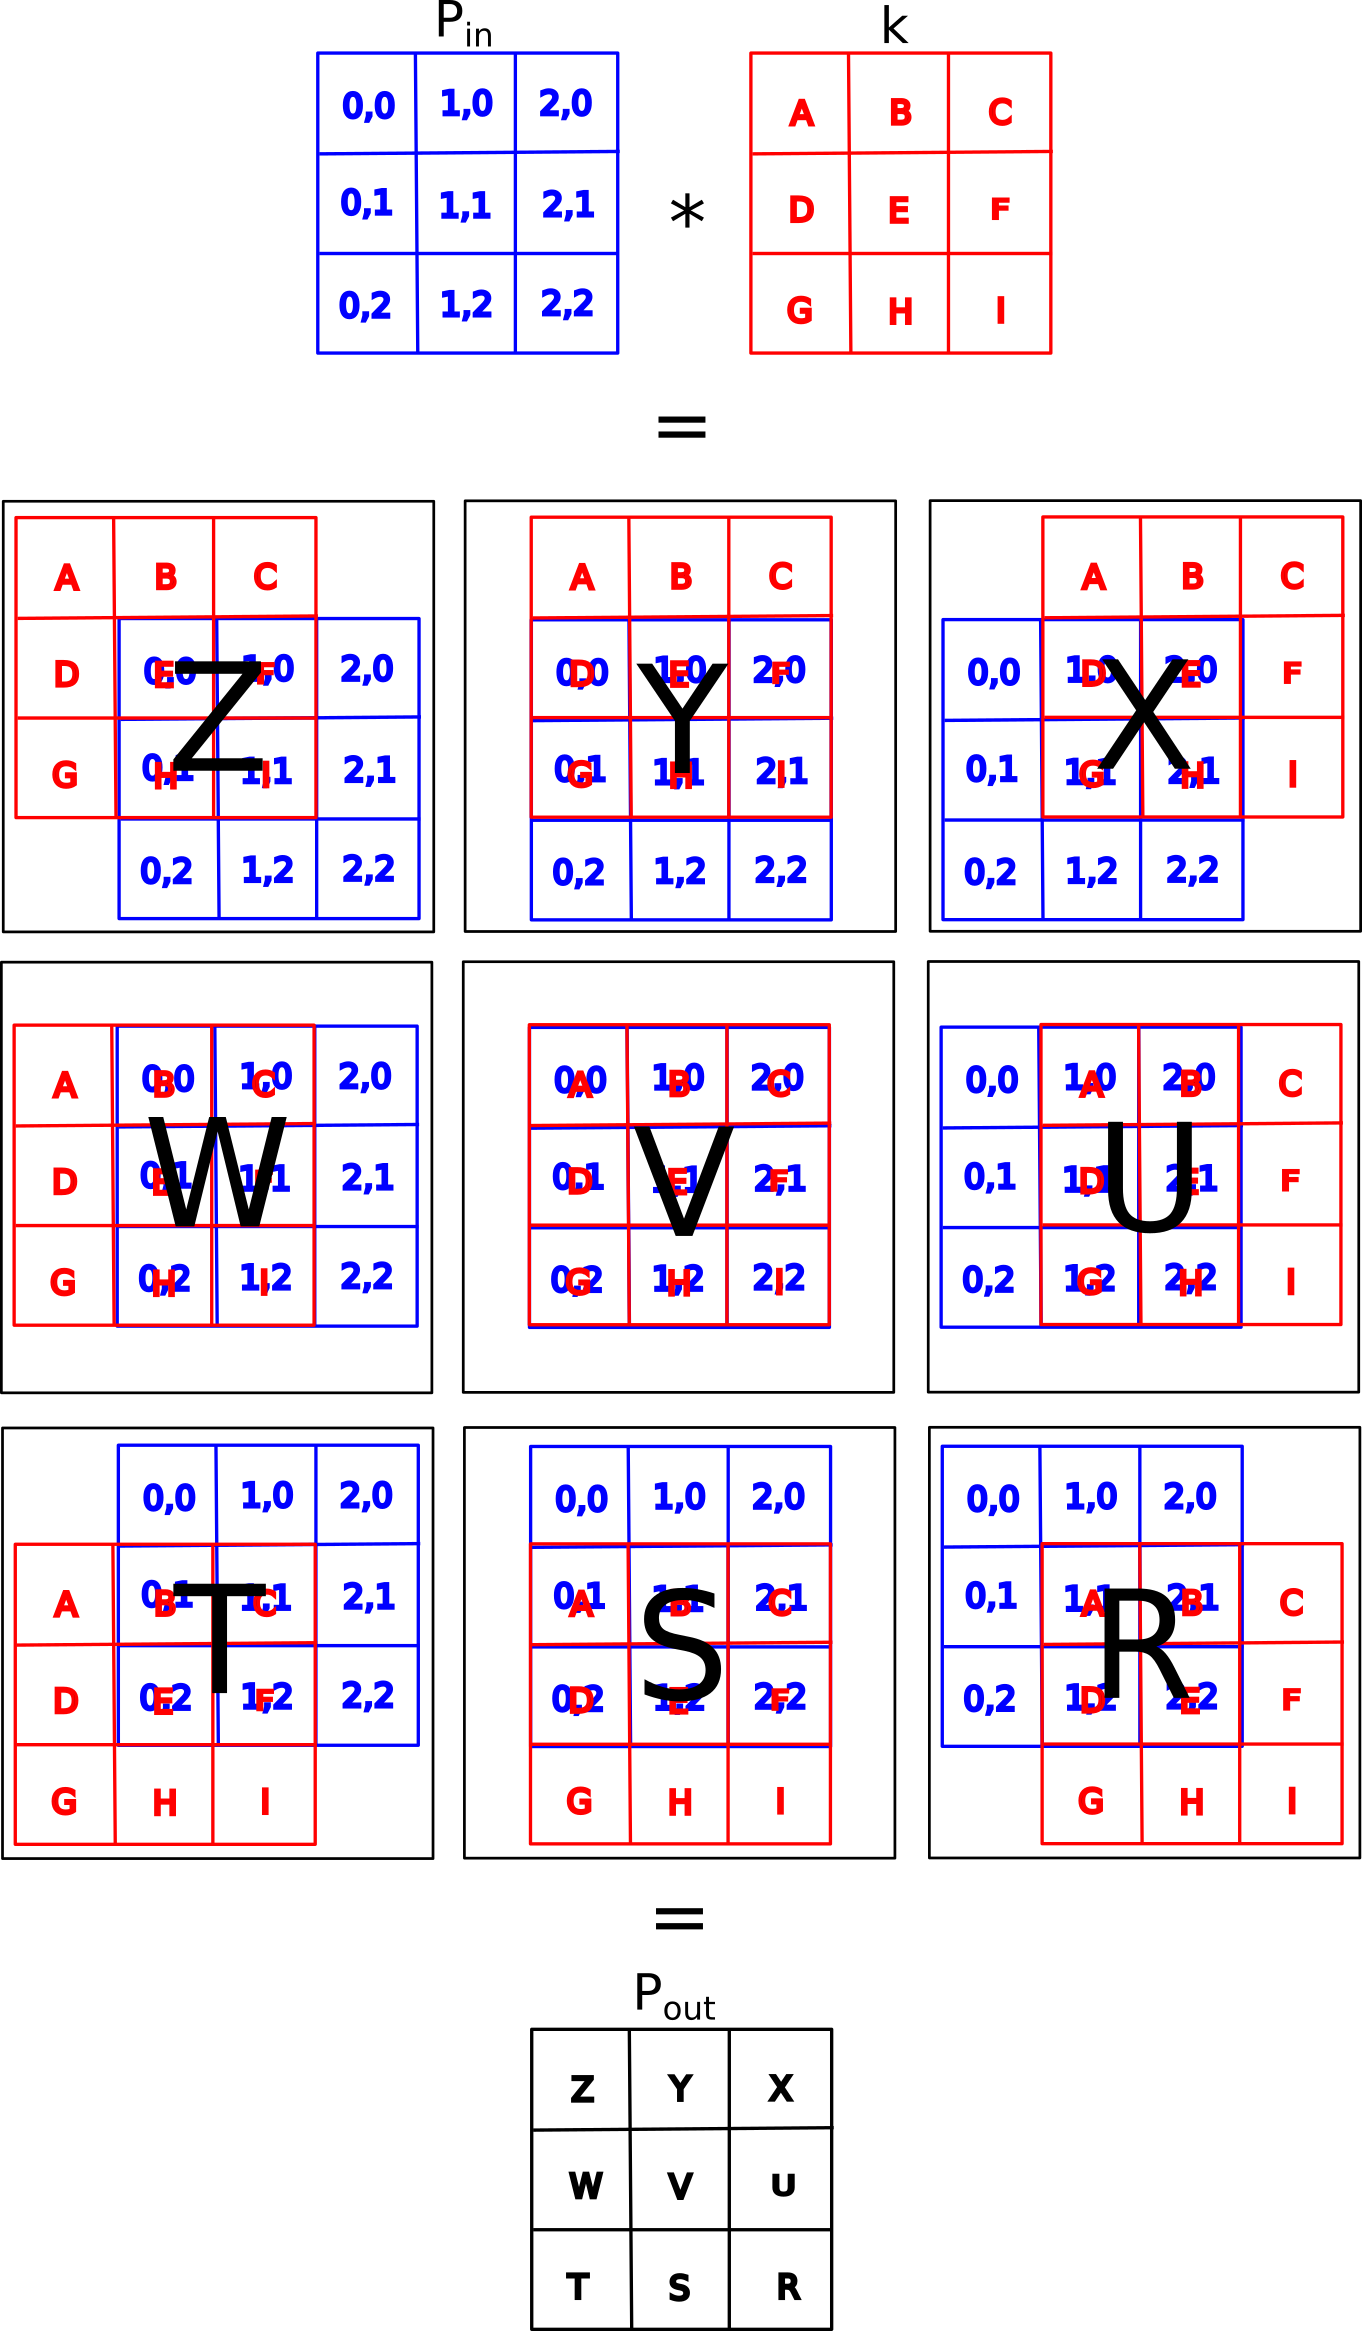
\includegraphics[width=0.75\textwidth]{Figs/intro2dl/convolution.png}
	\caption{An example of convolution of a (3x3) array with a (3x3) kernel.}
	\label{fig:convolve}
\end{figure}


To implement convolution effciently, the kernel is flattened and then zero padded forming a 9x9 matrix, so that every convolution step can be performed in a single matrix multiplication. \autoref{fig:convImpl} demonstrates this. Note that the input array is also flattened. 

This results in the multiplcation (9x9)x(9x1) = (9x1) which can then be reshaped to be (3x3) again.

\begin{figure}
	\centering	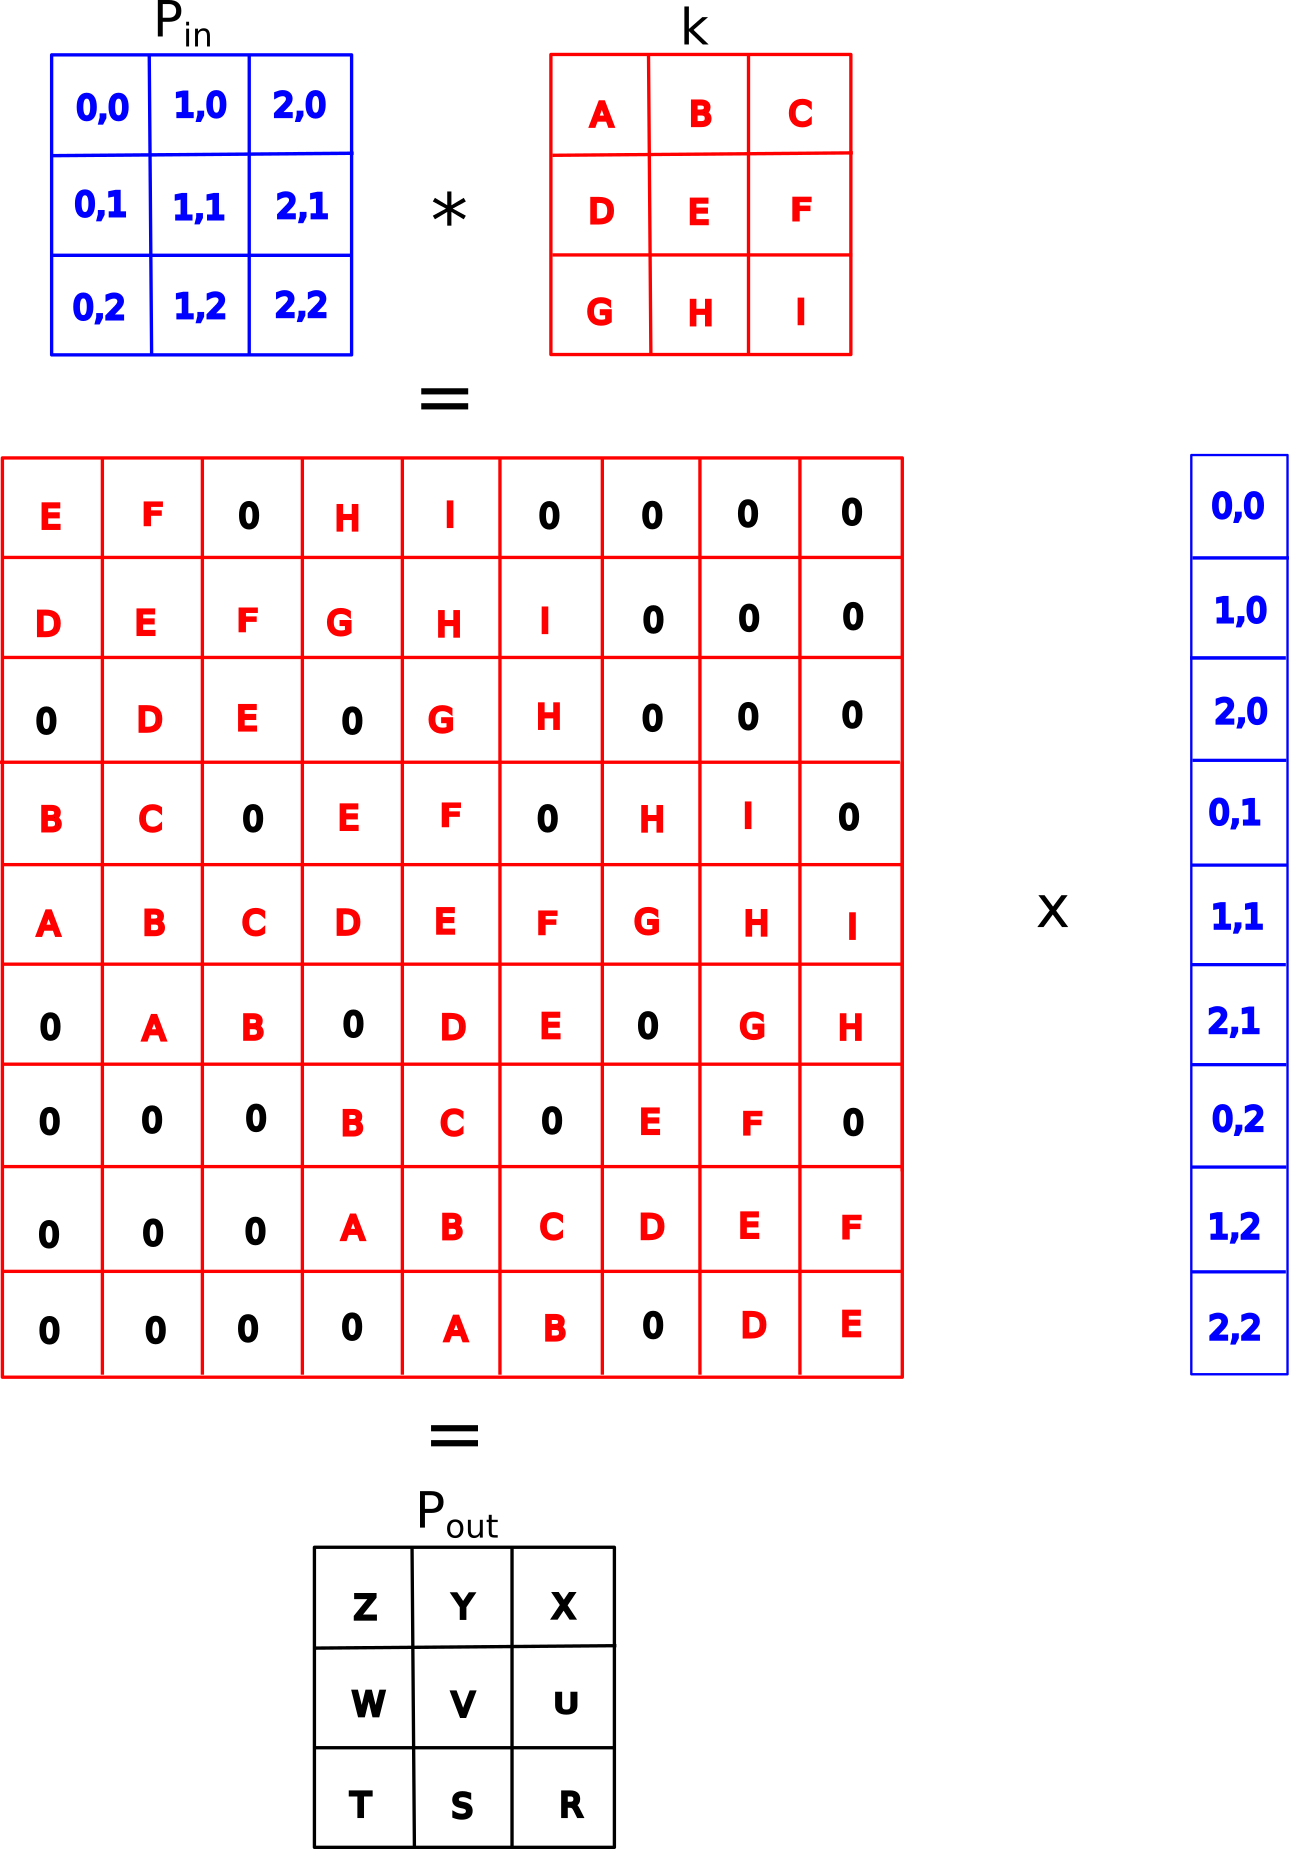
\includegraphics[width=0.75\textwidth]{Figs/intro2dl/convolutionImplementation.png}
	\caption{The implementation of the convolution of a (3x3) array with a (3x3) kernel.}
	\label{fig:convImpl}
\end{figure}

\subsection{Using Convolution Kernels in a Neural Network}
In a ConvNet, the weights of the network are kernels used to perform the convolution. Whereas, in a dense network, every input is connected to every neuron in the first layer and every neuron in the first layer is connected to every neuron in the second layer etc. each with their own individual weight, in a ConvNet, the weights are grouped into kernels and each neuron has it's own kernel which is applied across the entire input via the convolution opperation.

Any given layer in a dense network will have $(Data Dimensions) \times (Number of Neurons)$ weights. The convolutional equivalent will have $(Kernel Size) \times (Number of Neurons)$ weights, usually this will be far fewer than the dense network. This gives a significant increase in computational performance.

For each neuron in a ConvNet, a single matrix multiplcation like that shown in \autoref{fig:convImpl} is performed \endnote{In the case of image data where pixels have 3 channels (RGB) 3 multiplcations are performed, one between the kernel (k) and each channel which are then summed to give a single output. $R\times k + G\times k + B\times k$}.

\subsubsection{Strided Convolution}
In \autoref{fig:convolve}, convoltuion was performed with a stride of one. Strided Convolution refers to the case where the stride, the number of spaces between each application of the kernel, is greater than one. For example, convolution of an image and a kernel with a stride of two would be the convolution of the kernel with every other pixel of the image and would result in an output $\frac{1}{4}$ the size of the input (half the width by half the height).

Altering the stride of a convolution is very useful for performing down sampling. Down sampling reduces the computational burden of a system by reducing the amount of calculations that need to be performed.

Alternatively, strided convolutions can be used to up sample data by making use of a fractional stride. For example a stride of $\frac{1}{2}$ when convolving a kernel and an image would result in an output 4 times the size of the input ($2\times$ the width by $2\times$ the height).

Fractionally strided convolutions can be used for many things including image enhancement \cite{radford2015unsupervised} and, as in this thesis, to rescale data back up to its original size.

\subsection{Transposed Convolutions}
Fractionally strided convolution is the inverse of a strided convolution whose strides are reciprocals (e.g. $\frac{1}{2}$ vs. 2), with respect to the scale of the data. However, having an inverse of the convolution with respect to the contents of the data is also necessary.

This is where transposed convoltuion comes into play \cite{zeiler2010deconvolutional}. 

Transposing a matrix, for example a convolution kernel, has the effect of rotating it by 90 degrees. Understanding why doing this before performing a convolution has the effect of reversing the convolution requires first understanding how convolution is performed on a computer.

As shown in \autoref{fig:convImpl} the actual convolution operation involves flattening and reshaping the kernel. Transposing this flattened and reshaped kernel allows for the recovery of the original input as shown in \autoref{fig:transConvImpl}. 

\begin{figure}
	\centering	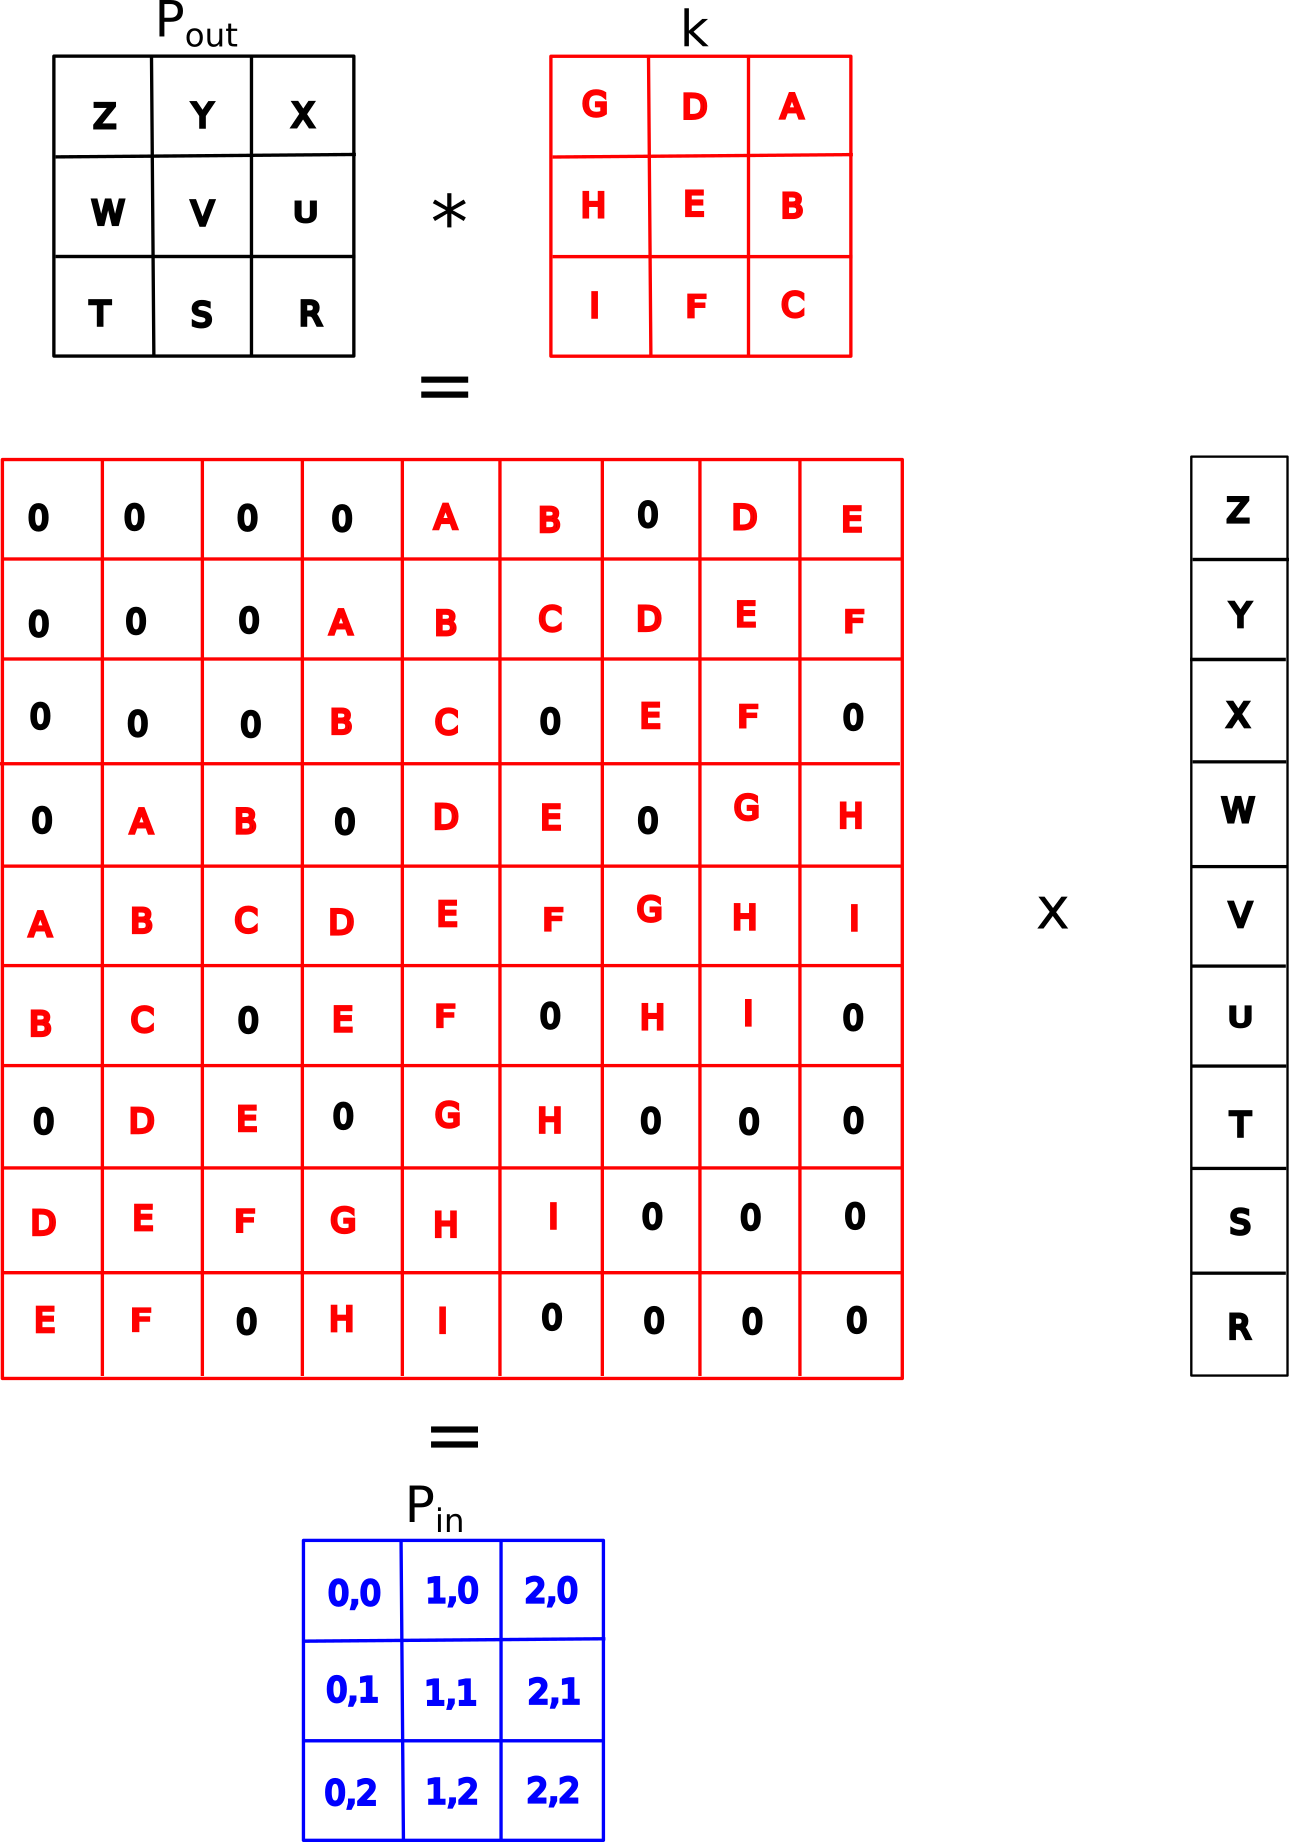
\includegraphics[width=0.75\textwidth]{Figs/intro2dl/TransconvolutionImplementation.png}
	\caption{The implementation of the transposed convolution of a (3x3) array with a (3x3) kernel.}
	\label{fig:transConvImpl}
\end{figure}

This results in the multiplcation (9x9)x(9x1) = (9x1) which can then be reshaped to be (3x3) again. However, this doesn't really highlight what has happened due to the symmetrical shape of the kernel and input. Consider the multiplcation of (4x16) kernel with a flattened 16x1 array. The convolution gives a (4x1) output. Transposing the kernel to be (16x4) and multiplying with the (4x1) output gives the (16x1) flattened array. 


%\section{Recurrent Neural Networks}
%\subsection{Vanilla RNN}
%\subsection{Gated RNN}
%
%\begin{figure}
%	\centering
%	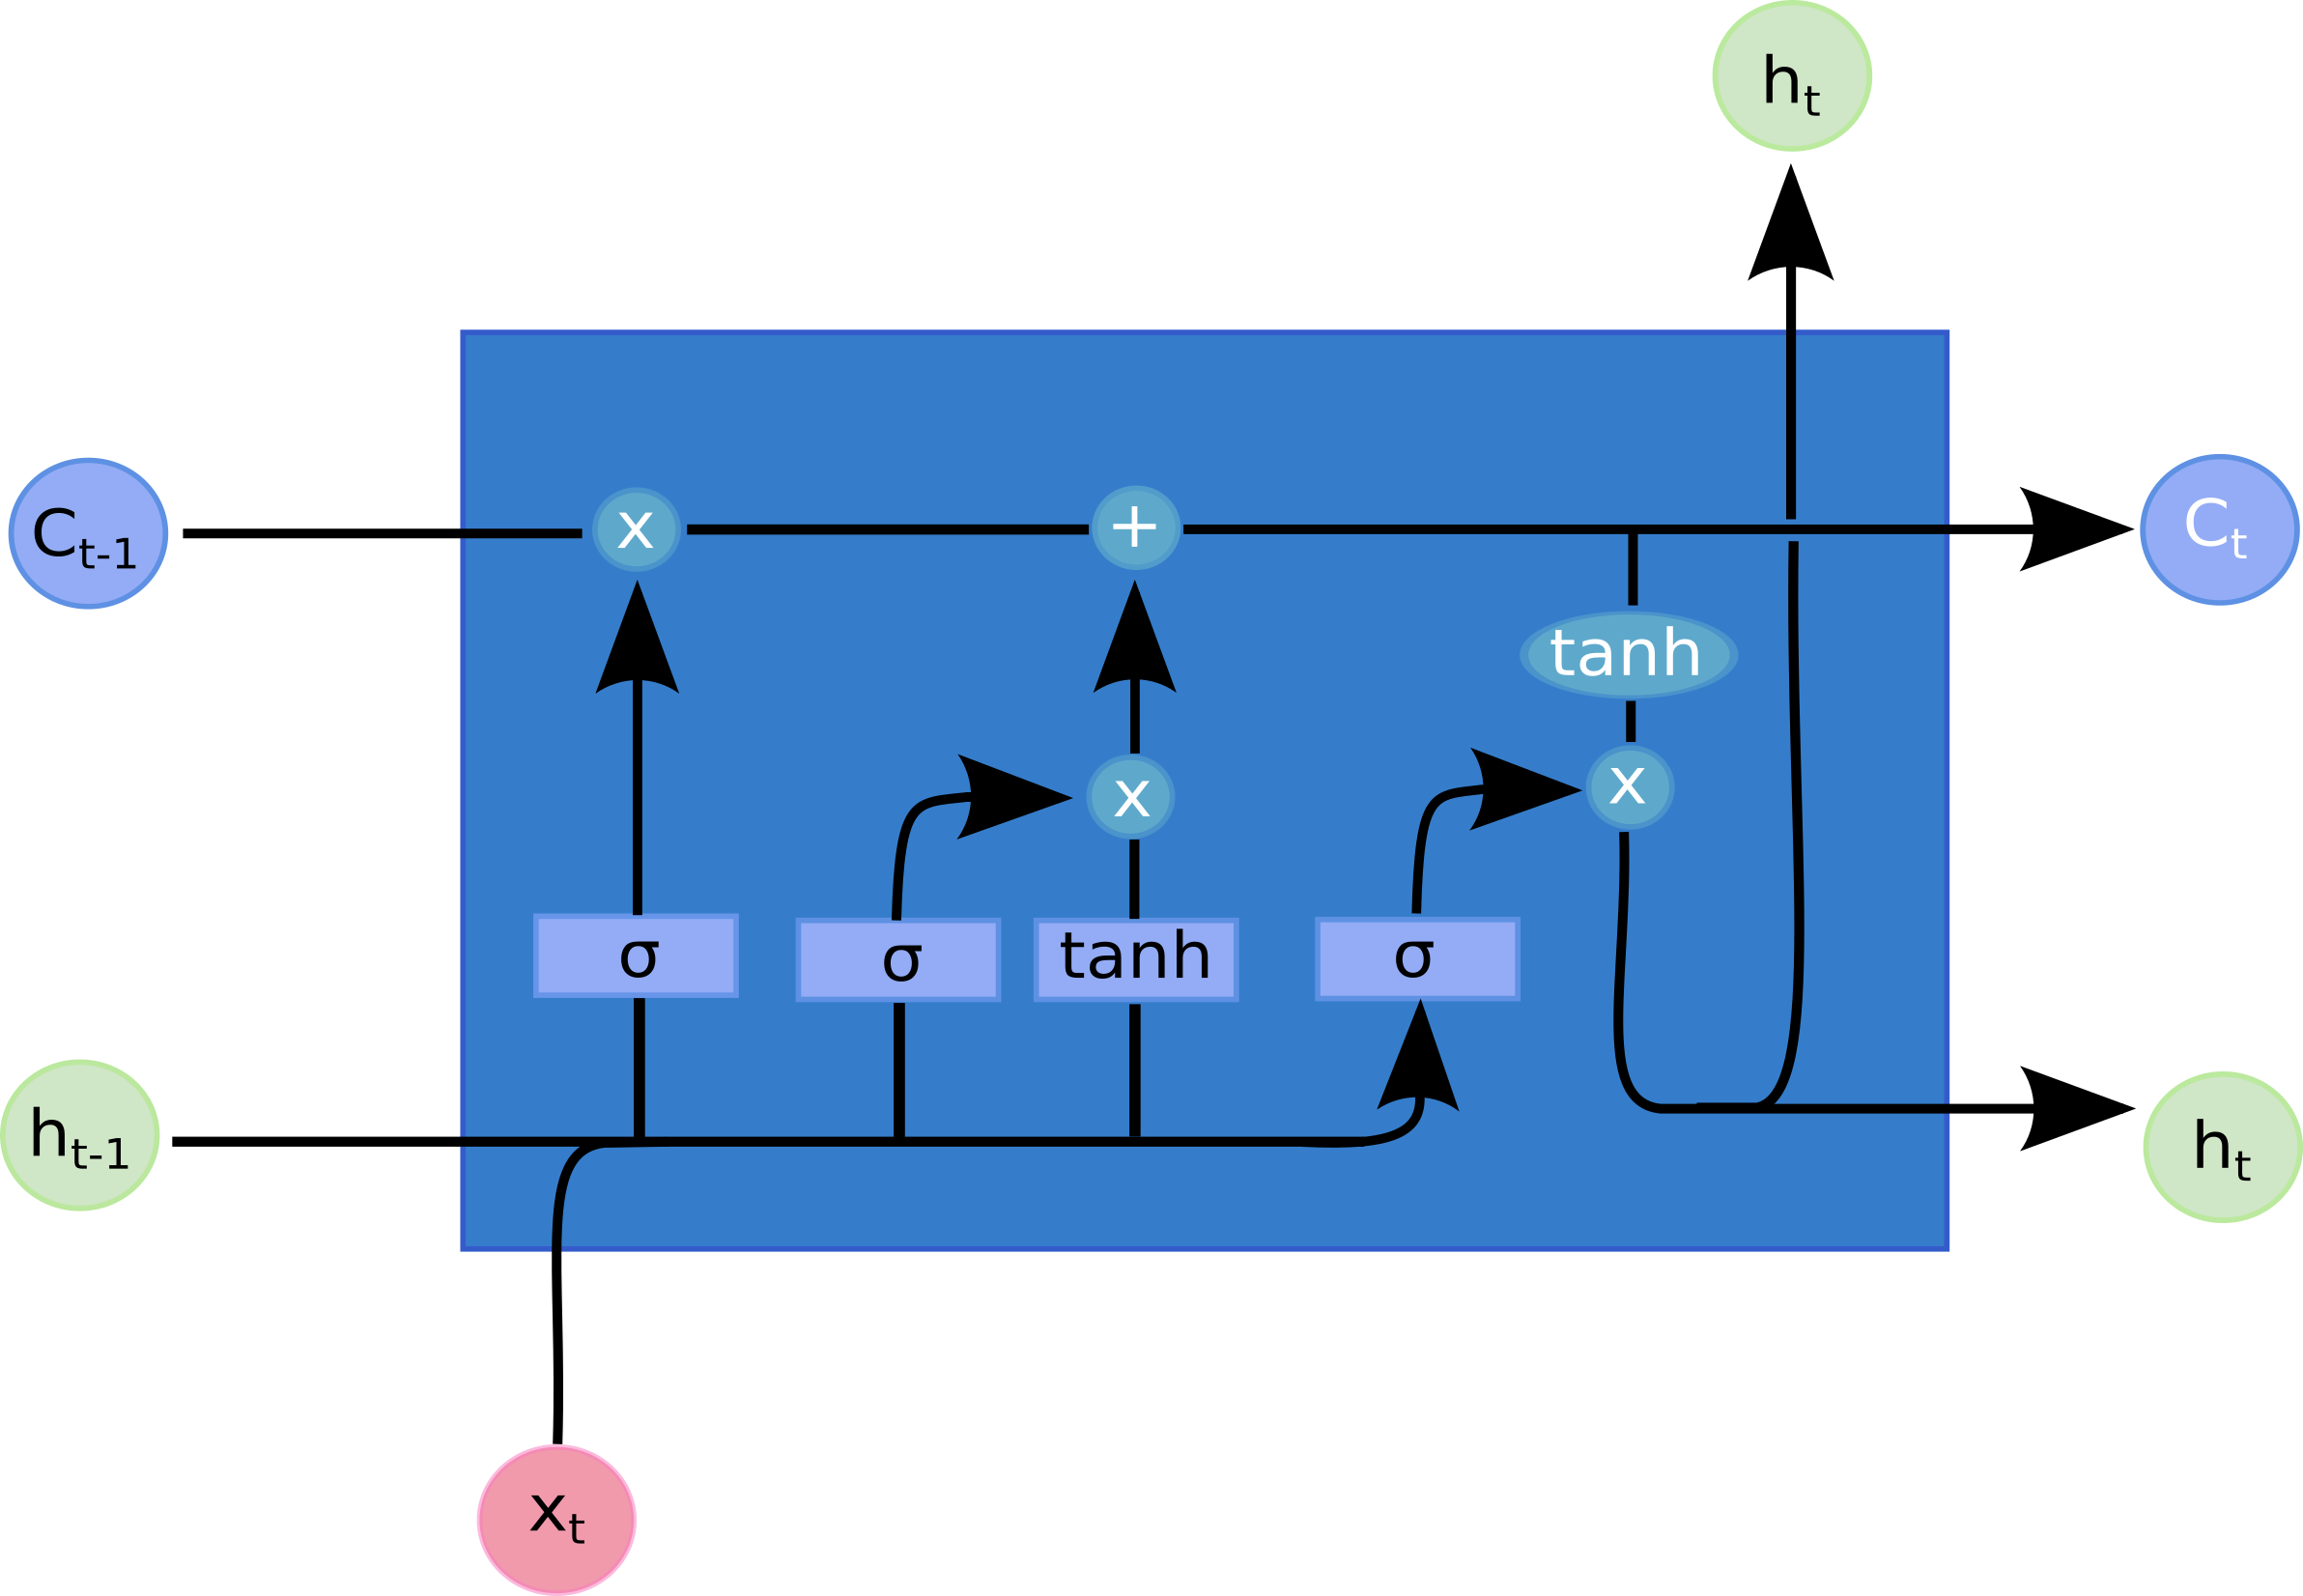
\includegraphics[width=0.5\textwidth]{Figs/intro2dl/LSTM.png}
%	
%	\caption{A Long Short-Term Memory Unit}
%	\label{fig:lstm}
%\end{figure}
%
%\begin{figure}
%	\centering
%	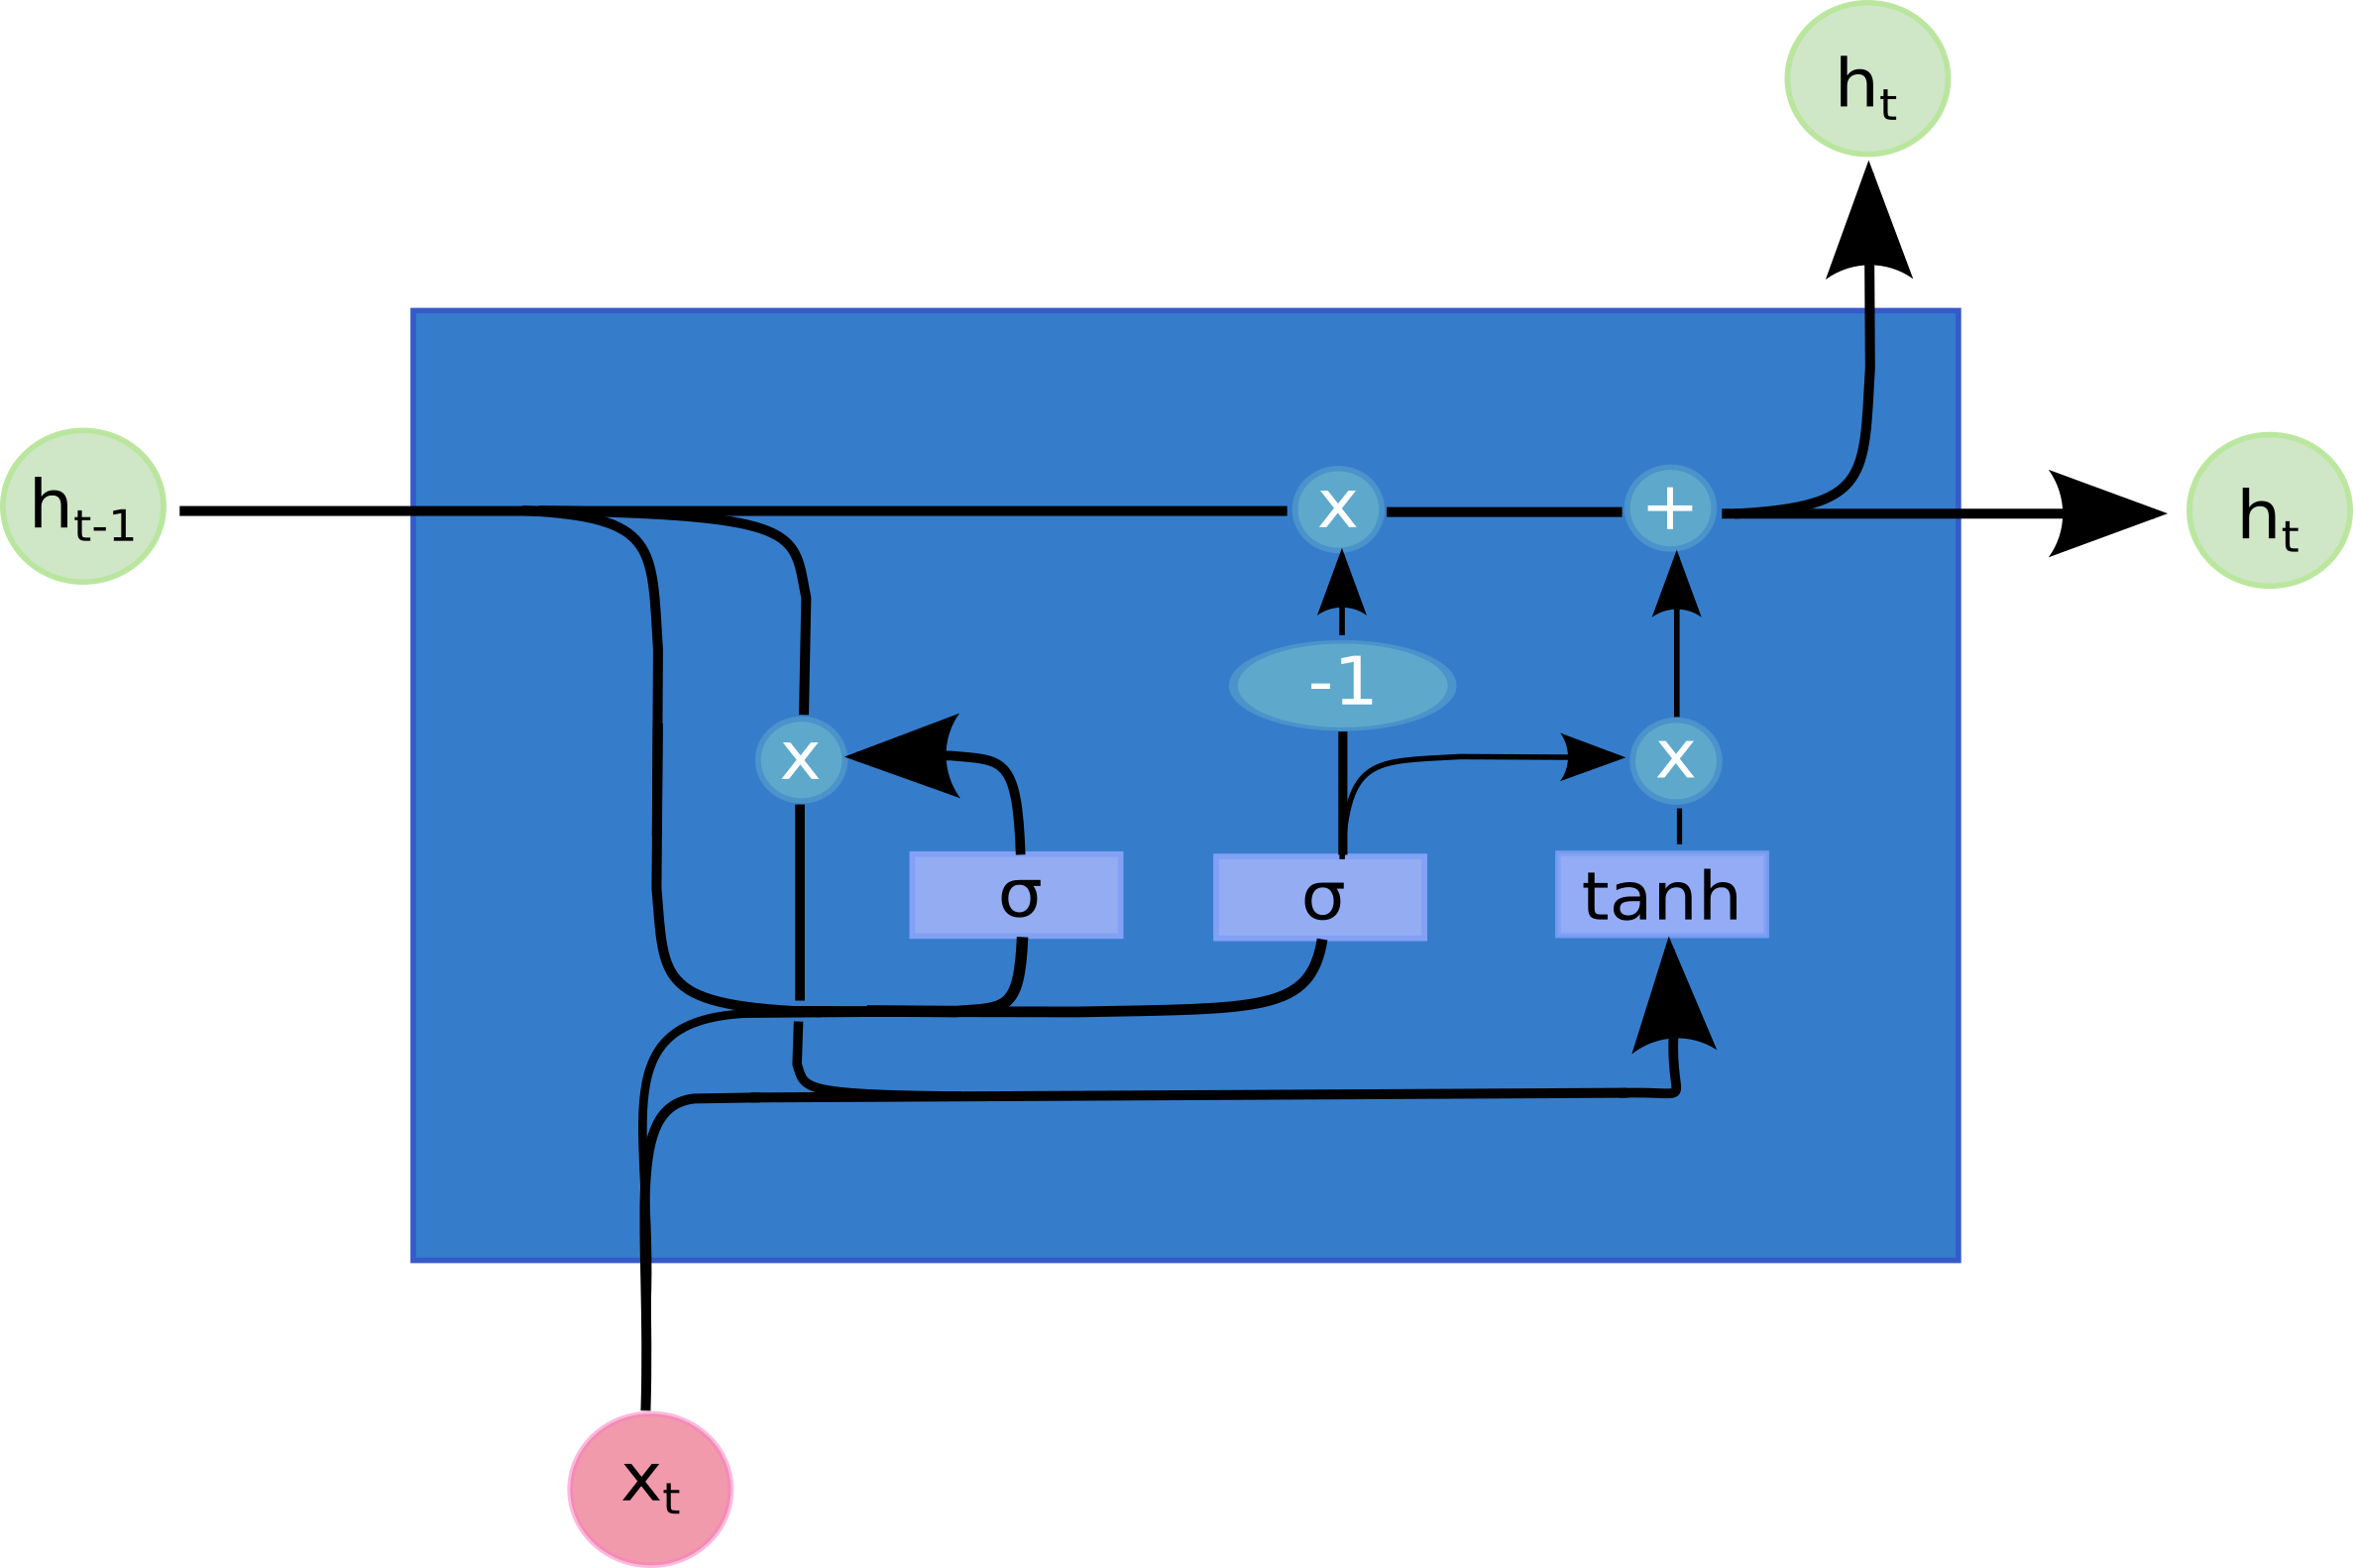
\includegraphics[width=0.5\textwidth]{Figs/intro2dl/GRU.png}
%	
%	\caption{A Gated Recurrent Unit}
%	\label{fig:gru}
%\end{figure}

\section{Autoencoders}
Autoencoders (AE) can be constructed from any type of neural network layers, ConvNet, LSTMs, or Dense to name a few. What makes an AE an AE is not the type of layers from which it is constructed but the way in which it is trained.

An AE is trained to reproduce its input at its output (\autoref{fig:ae}. Typically, dimensional reduction is applied within the AE so that it must learn to select the most important features of the input data to accuartely represent the data in a more compressed form. 

I make use of strided convolutions for dimensional reduction in the encoder and fractionally strided convolutions for dimensional enlargement in the decoder of the MAEs trained in this thesis.

\begin{figure}
	\centering
	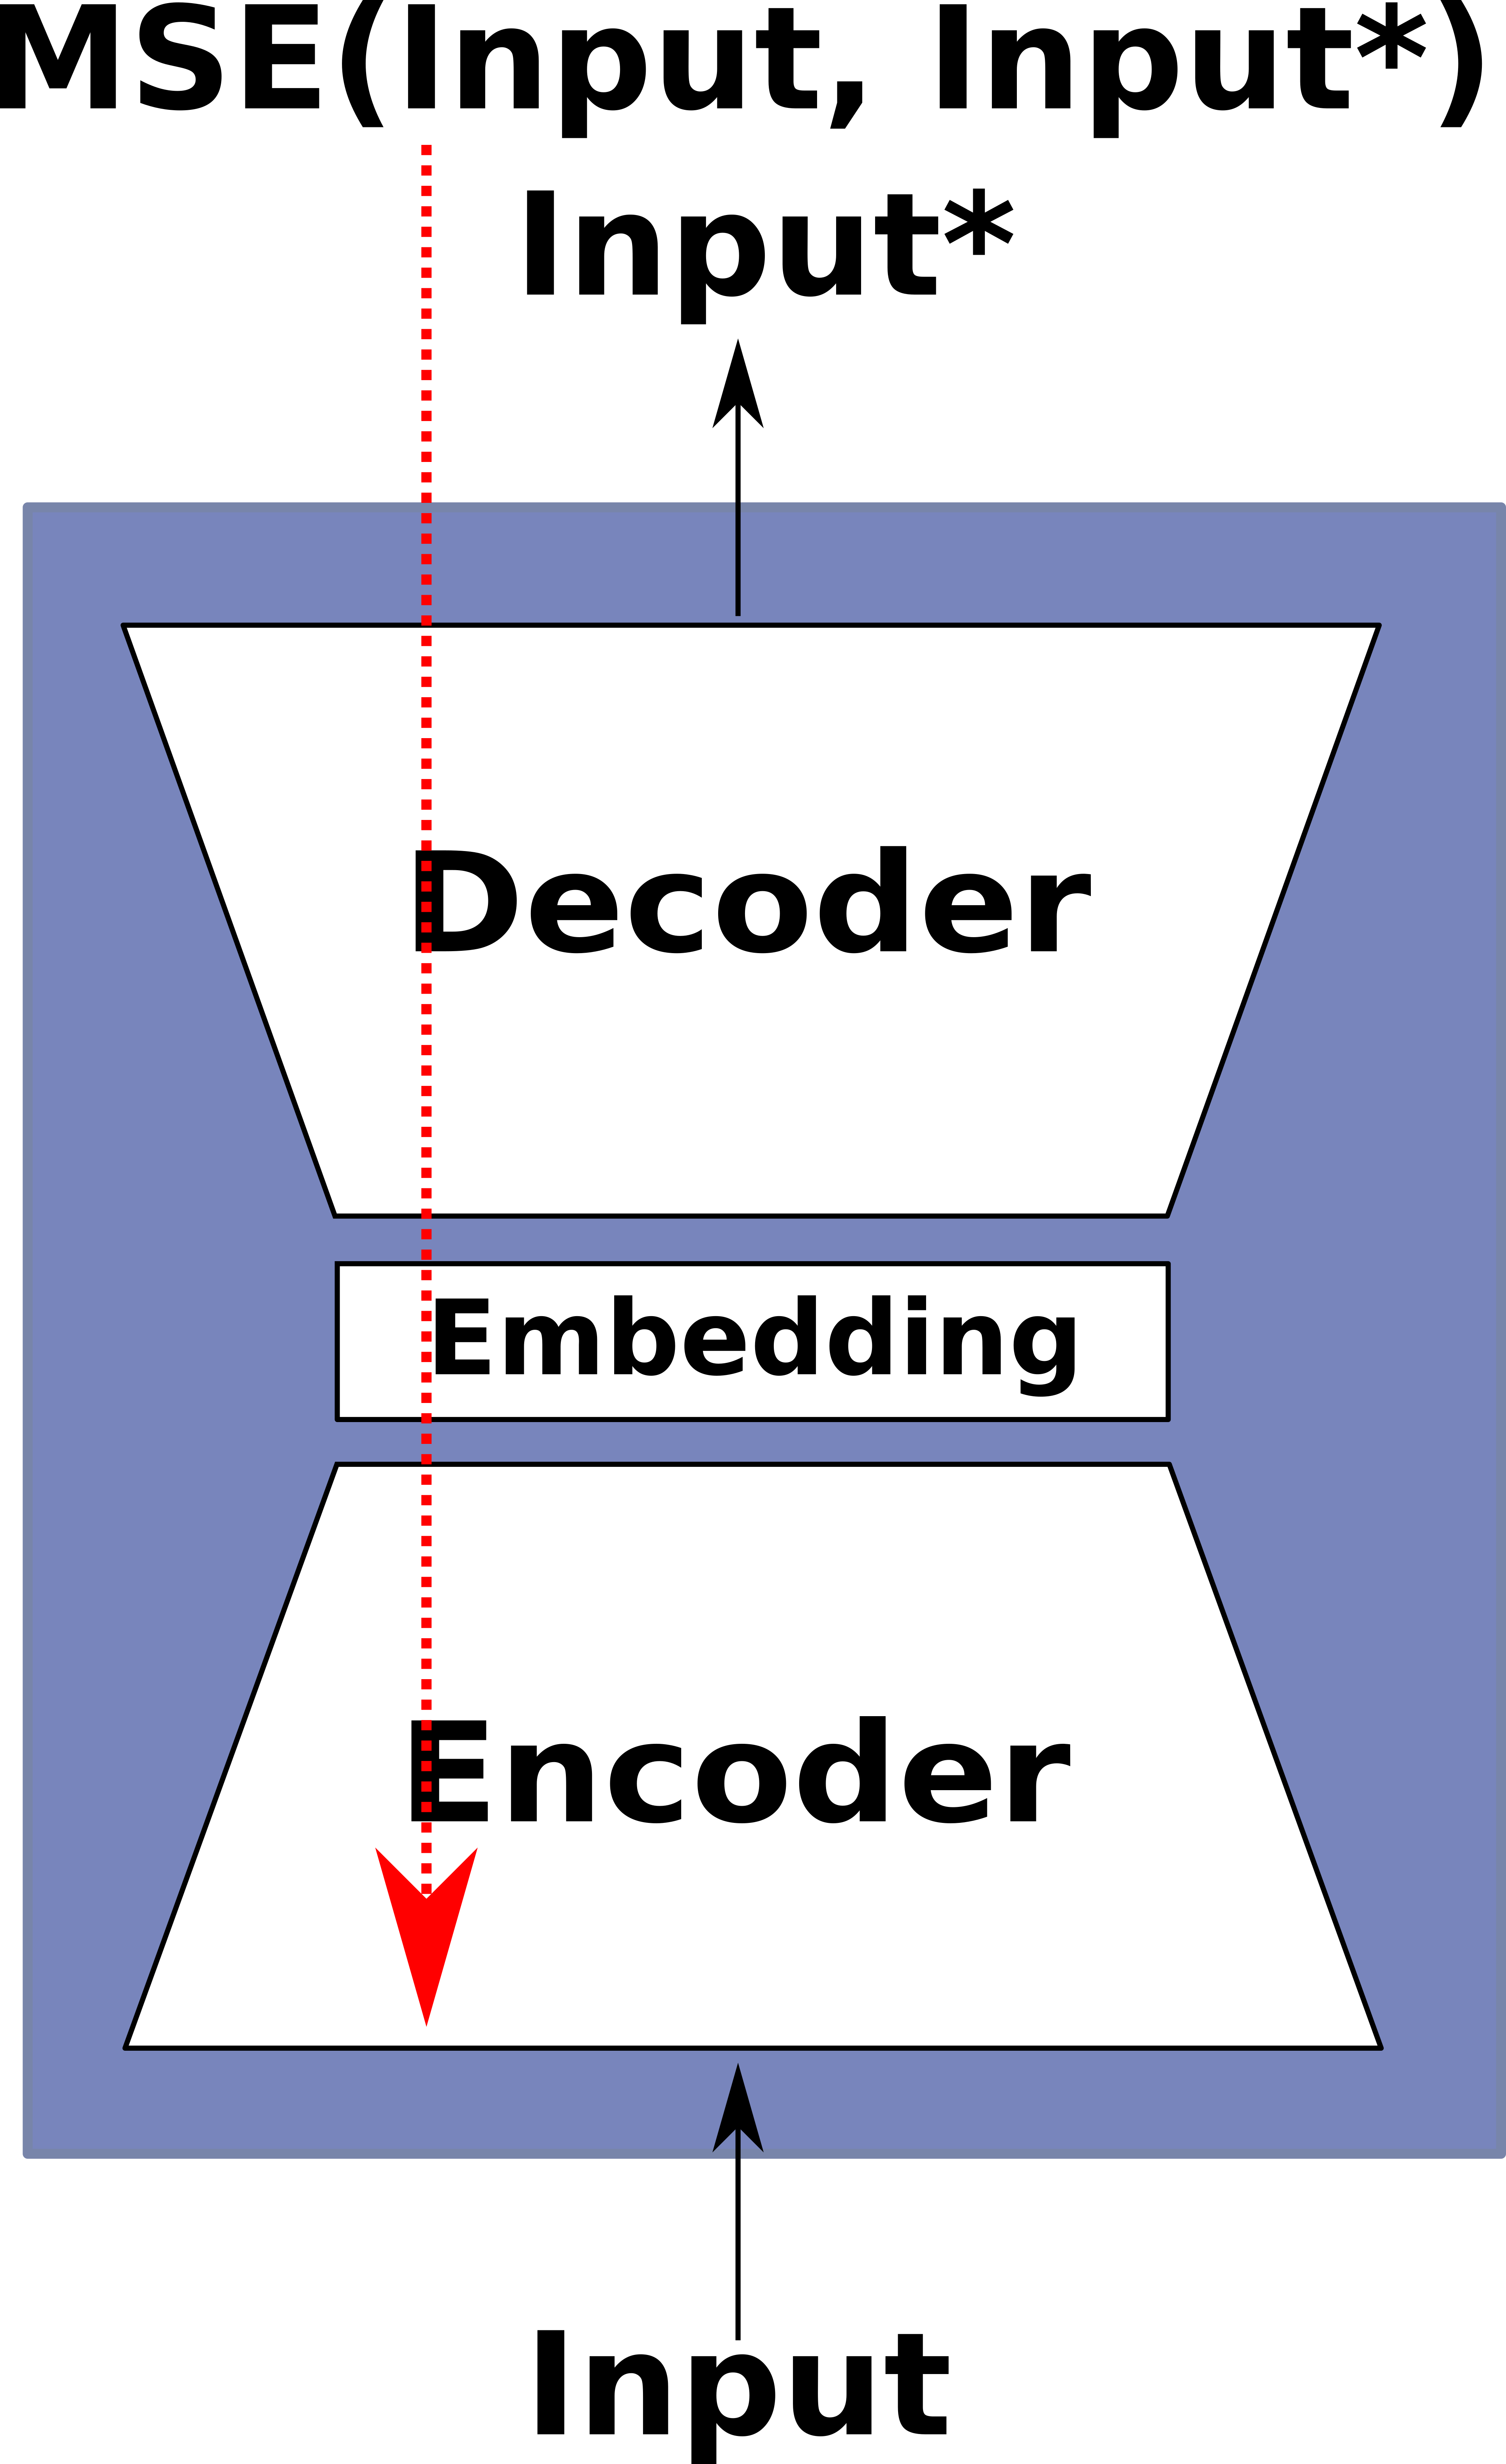
\includegraphics[width=0.25\textwidth]{Figs/intro2dl/AE.png}
	
	\caption{An Autoencoder trained using the MSE of its input and reconstruction of the input (Input*). The red arrow shows how the error is backpropgated through the network.}
	\label{fig:ae}
\end{figure}



\subsection{Variational Autoencoders}
An important enhancement of AEs is the Variational Autoencoder (VAE). The VAE is trained using a multipart cost function. A normal cost such as MSE plus the KLD of the embedding from a target distribution (usually a Gaussian).

This has the effect of forcing the embedding space to be smooth and helps to stop discontinuities in the embedding from occuring. For example, if a particular part of the embedding space is never explored in an AE, the output generated by the decoder can be unpredictable even for embeddings close to those seen from training data. In a VAE, due to the extra constraint placed on the embedding space, the generated output will change smoothly as the embedding is altered smoothly.


\subsection{Multimodal Autoencoders}
Multimodal Autoencoders (MAE) operate similarly to AEs however, they take two or more modalities as input. In this thesis, only bimodal MAEs are used though in principle, MAEs are not limited to only two modalities.

The MAE is trained to reproduce all modalities regardless of whether all modalities are present at the input. For example, if a bimodal MAE takes images and text as inputs, it is trained to reproduce images and text from it's inputs. However, if only an image is available as input, the MAE is still trained to produce an image and the aligned text or vice versa when only text is available.


\begin{figure}
	\centering
	
\includegraphics[width=0.5\textwidth]{Figs/intro2dl/MAE.png}
	
	\caption{A Multimodal Autoencoder}
	\label{fig:mae}
\end{figure}

Each modality is encoded separately through its own branch of the network and then the embeddings are concatenated forming a joint embedding. The joint embedding is the used to reconstruct each modality through their own decoder branches as seen in \autoref{fig:mae}.

%
%\section{Summary}
%
%The most important points to take away from this section are:
%
%\begin{itemize}
%	\item Neural Networks consist of neurons each with their own respective weights.
%	\item The output of a neuron is proportional to its input multiplied by its weights.
%	\item Weights are trained using Gradient Descent and Backpropogation.
%	\item Gradient Decent requires a measure of error known as a cost function.
%	\item Gradient Descent can get stuck in local minima. Where the optimisation finishes is dependant on the training data, cost function and where the optimisation started.
%	\item ConvNets use Kernels of weights instead of being densely connected across their inputs.
%	\item AEs are trained to reproduce their input from a compressed representation.
%	\item MAEs are AEs which take multiple modalities as input creating a single embedding across the modalities.
%\end{itemize}

\theendnotes
%% Chapter Template
\chapter{A Primer on Artifical Neural Networks} % Main chapter title

\label{Chapter3} % Change X to a consecutive number; for referencing this chapter elsewhere, use \ref{ChapterX}

\lhead{Chapter 3. \emph{A Primer on Artifical Neural Networks}} % Change X to a consecutive number; this is for the header on each page - perhaps a shortened title

%----------------------------------------------------------------------------------------
%	SECTION 1
%----------------------------------------------------------------------------------------
\section{Introduction}
This chapter presents an overview of the mathematical theory behind artificial neural networks and how they learn. It should serve as a quick guide to the techniques used in the experiments within this thesis.

\section{Perceptrons}
\label{sec:percep}
The perceptron is the parent of modern artificial neurons \cite{rosenblatt1958perceptron}.
Perceptrons arranged in layers, referred to as multi-layer perceptrons, are therfore the predecessor of modern artificial neural networks.

\subsection{What is a Perceptron}



\begin{figure}
	\centering
	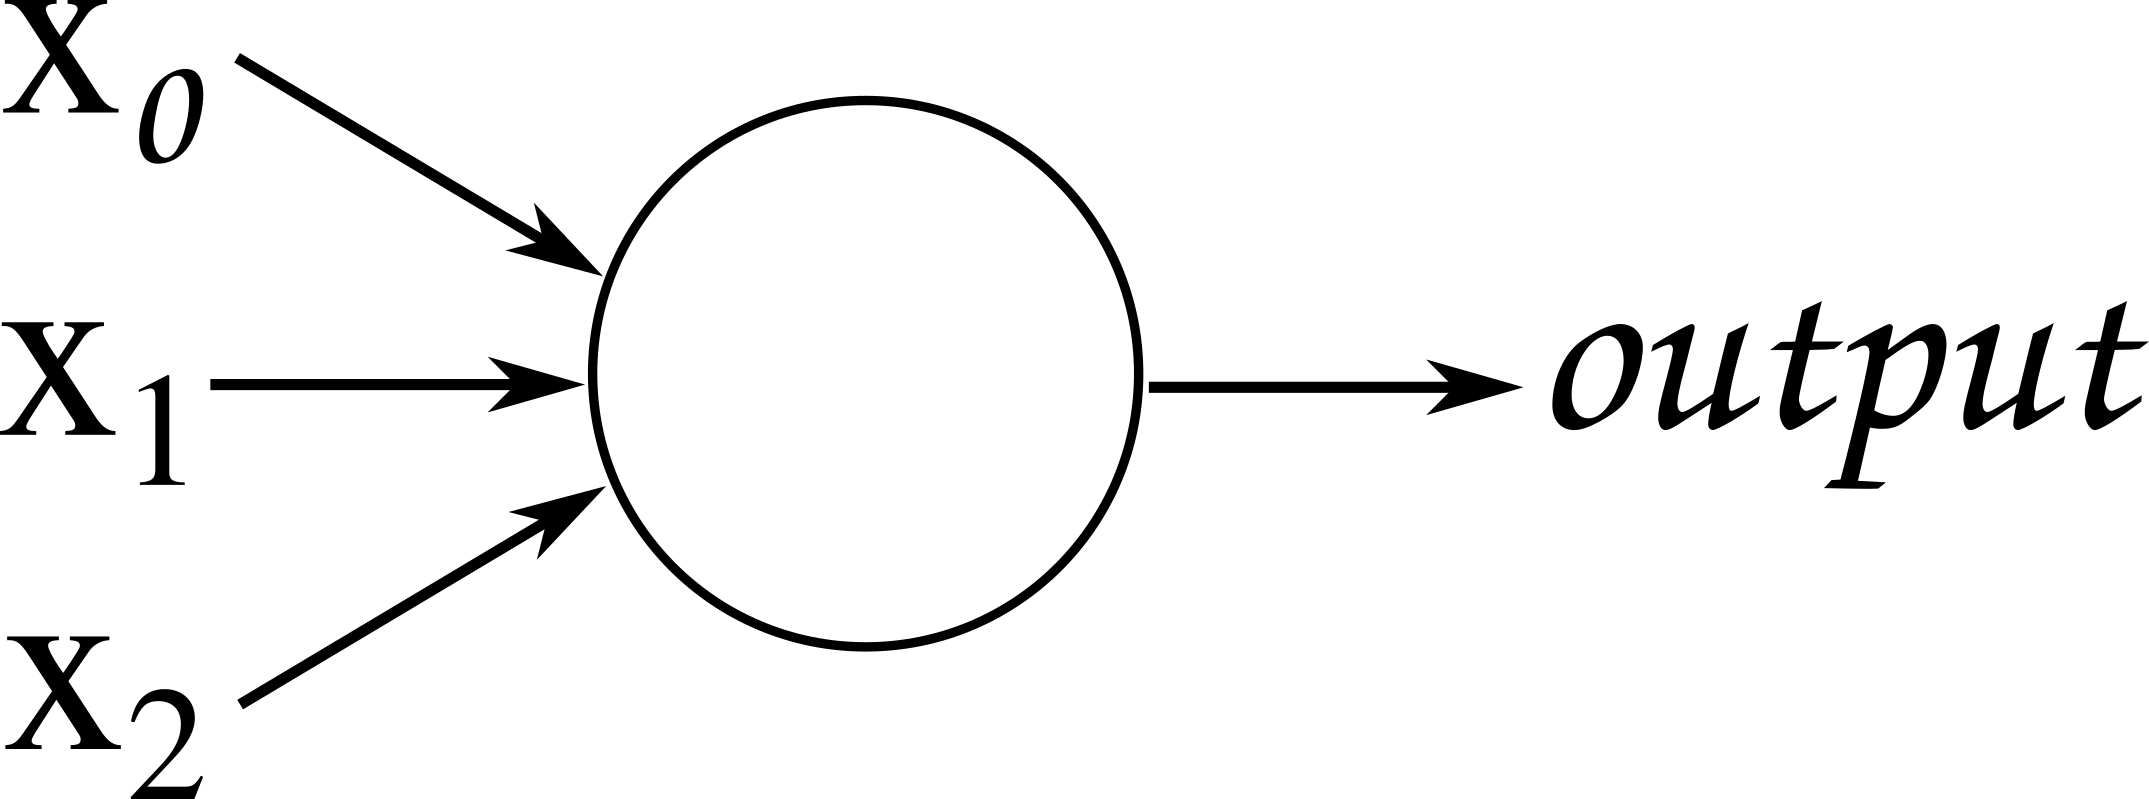
\includegraphics[width=0.5\textwidth]{Figs/intro2dl/perceptron.png}
	
	\caption{A perceptron with three binary inputs, $x_0, x_1, x_2$.}
	\label{fig:perceptron}
\end{figure}

Perceptrons are biologically inspired computation units and are a type of artificial neuron. They take a series of binary inputs, compute a weighted sum and produce a binary output based on the value of this sum as seen in \autoref{fig:perceptron}.


\begin{equation}
output = \begin{cases}
0 &\text{if $\sum_{j} w_j x_j + b < 0$}\\
1 &\text{if $\sum_{j} w_j x_j + b \geq 0$}
\end{cases}
\label{eqn:percep} 
\end{equation}

Where $x_j$ is the jth input, $w_j$ is it associated weight and $b$ is a constant value called the bias, which affects how easy it is for the neuron to activate. The output of the perceptron is caluclated using the formulation shown in \autoref{eqn:percep}.

By adjusting each of the weights we can change the output of the perceptron. For example, if we wanted to use a perceptron to decide whether to have a picnic today we can  select a set of relevant inputs, ``the weather is nice" and ``the pollen count is low".

If it is a sunny day, and the pollen count is high, the input to the perceptron would be $[1,0]$.
 
We will set our weights depending on how important each of the inputs is. No one likes a picnic in the rain, so the weather is important, whilst the pollen count is only important if you suffer from hayfever. We will select a bias of -5 for our perceptron.

For person A, the weights might look like $[7, 0]$ (person A doesn't suffer from hayfever). Therefore the output of the perceptron would be 1 as $1 \times 7 + 0 \times 0 - 5 = 2$ is greater than 0, so person A will go for a picnic.

Person B owns a large umbrella (so the weather doesn't matter as much) but they do suffer from hayfever, their weights might look like $[4, 7]$. The output of the perceptron would be 0 as  $1 \times 4 + 0 \times 7 - 5 = -1$ is less than 0. Therefore, person B would wait for a day with a lower pollen count for a picnic.


\subsection{Multi-Layer Perceptron}
In the previous section I demonstrated how a single perceptron can be used to make decisions based on a set of inputs. However, things get much more interesting when we start to link multiple perceptrons together into multi-layer perceptrons (MLP).

\begin{figure}
	\centering
	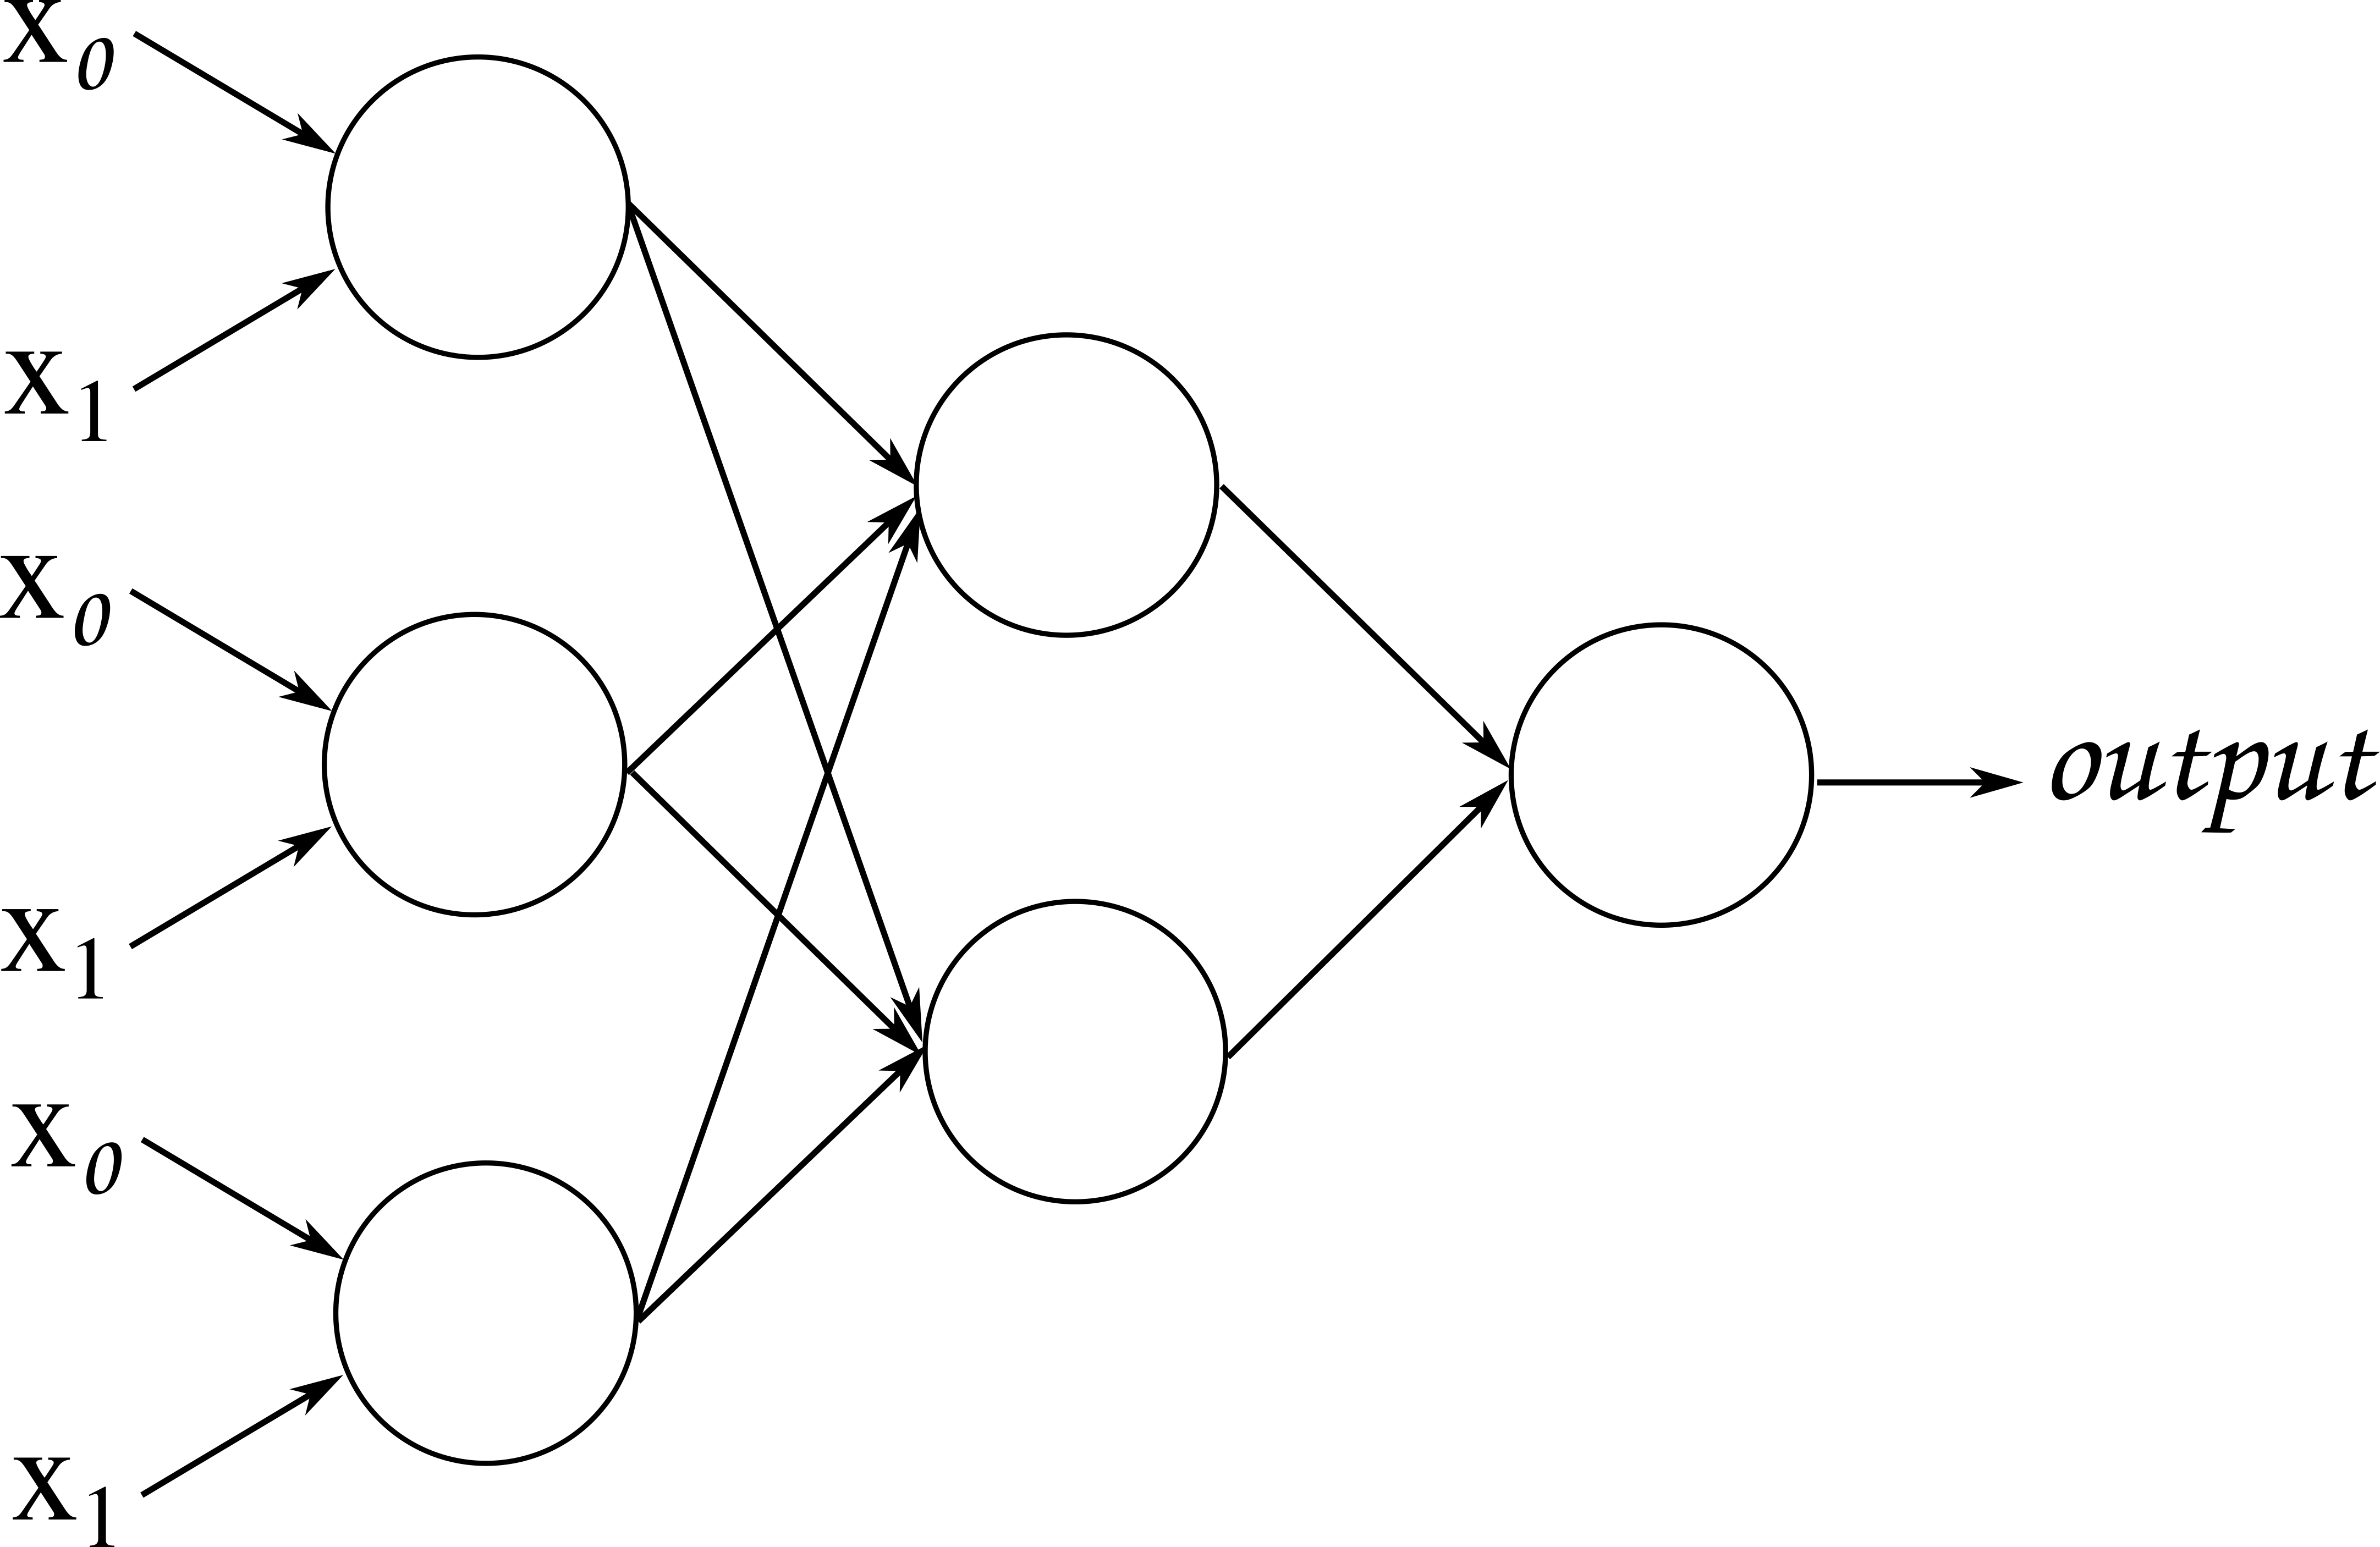
\includegraphics[width=0.5\textwidth]{Figs/intro2dl/mlp.png}
	
	\caption{A multi-layer perceptron consisting of three perceptrons arranged in two layers, with three binary inputs, $x_0, x_1, x_2$.}
	\label{fig:mlp}
\end{figure}

If we take the example from the previous section about deciding to go for a picnic or not, we can use the MLP shown in \autoref{fig:mlp} to consider what happens if person A and B want to go for a picnic together.

Given the previous conditions of a sunny day with a high pollen count, person A wants to go whilst person B does not, as demonstrated by the outputs of their individual perceptrons. Taking these outputs as inputs to the second layer of our MLP, we can see whether the picnic will go ahead.

This time we will set the weights of the second layer based on who shouts the loudest. In this case, person A really wants to go and is very vocal about it. $1 \times 9 + 0 \times 5 - 5 = 4$ so the picnic will go ahead. This resulted in person B developing a headache and sneezing a lot. Clearly we need to find a way to adjust the weights of our MLP so that it makes better decisions in the future.

\section{Activation Functions}

Only being able to handle binary values is a major drawback of the perceptron. An artificial neuron which can handle continuous values is much more useful.

This limitation occurs due to the activation function of the perceptron shown in \autoref{eqn:percep}. Visualising the perceptron activation function highlights that changes in the output of the neuron are not proportional to changes in the weights of the neuron as seen in \autoref{fig:activation_percep}. With a few small changes we can make an artifical neuron that accepts continuous values and has a continuous output.

\begin{figure}
\begin{center}
\begin{tikzpicture}

% Us


\begin{axis}[
axis lines=middle,
xtick={-10,0,10},
xticklabels={$-\infty$, 0, $\infty$},
xlabel={$\sum_{j} w_j x_j + b$},
ylabel={Output},
xlabel near ticks,
ylabel near ticks]
\addplot +[blue, thick, mark=none] coordinates{(-10,0) (0,0) (0,1) (10,1)};

\end{axis}

\end{tikzpicture}
\caption{Visualisation of the perceptron activation function.}
\label{fig:activation_percep}
\end{center}
\end{figure}

A continuous output is very important as it means that a small change in the weights of a neuron will cause a small change in its output. This makes it much easier to understand how changing the weights affects the output of the network as the change in output becomes proportional to the change in weights as shown in \autoref{eqn:proport}

\begin{equation}
	\delta Output \propto \delta W
	\label{eqn:proport}
\end{equation}  


\subsection{Sigmoid Neurons}

The sigmoid neuron uses the sigmoid function, shown in \autoref{eqn:sig} as its activation function. 

\begin{equation}
\sigma(z) = \frac{1}{1 + e^{-z}}
\label{eqn:sig}
\end{equation}

$z$ is the sum of the weights multiplied by their respective inputs as seen in  \autoref{eqn:z_act}.

\begin{equation}
z = \sum_{j} w_j x_j + b
\label{eqn:z_act}
\end{equation}

As we can see in \autoref{fig:activation_sigmoid}, as $z$ changes, their is a proportional change in the output $\sigma(z)$, unlike in \autoref{fig:activation_percep} where the output only changes when $z$ crosses the y-axis.

\begin{figure}
\begin{center}
\begin{tikzpicture}



\begin{axis}[
axis lines=middle,
xtick={-10,0,10},
xticklabels={$-\infty$, 0, $\infty$},
xlabel={z},
ylabel={$\sigma$(z)},
xlabel near ticks,
ylabel near ticks]
\addplot[blue, thick, smooth, samples=1000, domain=-10:10]{1 / (1 + e^-x)};

\end{axis}
    

\end{tikzpicture}
\caption{Visualisation of the sigmoid activation function.}
\label{fig:activation_sigmoid}
\end{center}
\end{figure}

Now that we have an activation function that can produce continuous values, we can consider a much more diverse range of data to train our neural networks with. So instead of just making yes or no decisions we can look at, for example, the colours of pixels and decide if there is a cat in the image or given todays weather, predict if it will rain tomorrow.

\subsubsection{Other activation functions}
There are two other important and commonly used activation functions, though many others exist. These are, the hyperbolic tangent (Tanh) shown in \autoref{fig:activation_tanh} and rectified linear unit (Relu)  shown in \autoref{fig:activation_relu}.

\begin{figure}[h]
\begin{center}
\begin{tikzpicture}
\begin{axis}[
axis lines=middle,
xtick={-10,0,10},
xticklabels={$-\infty$, 0, $\infty$},
xlabel={z},
ylabel={$\sigma$(z)},
xlabel near ticks,
ylabel near ticks]
\addplot[blue, thick, smooth, samples=100, domain=-10:10]{tanh(x)};

\end{axis}
    

\end{tikzpicture}
\caption{Visualisation of the hyperbolic tangent activation function.}
\label{fig:activation_tanh}
\end{center}
\end{figure}

The Tanh function looks similar to the sigmoid function, however it has an output between negative one and one, where the sigmoid goes from zero to one. This is useful when having negative values within the network is important.

\begin{figure}[h]
\begin{center}
\begin{tikzpicture}
\begin{axis}[
axis lines=middle,
xtick={-10,0,10},
xticklabels={$-\infty$, 0, $\infty$},
xlabel={z},
ylabel={$\sigma$(z)},
xlabel near ticks,
ylabel near ticks]
\addplot[blue, thick, smooth, samples=1000, domain=0:10]{x};
\addplot[blue, thick, smooth, samples=1000, domain=-10:0]{0};

\end{axis}
    

\end{tikzpicture}
\caption{Visualisation of the rectified linear unit activation function.}
\label{fig:activation_relu}
\end{center}
\end{figure}

The Relu was created to address and issue known as vanishing gradients. This is to do with how neural networks are trained, as expalined in the next section. Briefly, as training depends on error gradients, having a linear activation function means that deeper networks \footnote{Deeper networks are beneficial as they can make more complex decisions by layering more and more simple decsions as shown in the MLP example in \autoref{sec:percep}} can be trained as non-linear functions like the sigmoid or Tanh will have reduced gradient magnitude when they are differentiated to backpropogate the error through the network. If that doesn't make sense yet, don't worry, it will become clear shortly.

\section{Learning Algorithms}
In \autoref{sec:percep} we saw how simple computation units can make simple decisions and how these can be chained together to make more complex decisions. However, sometimes the decisions we make are wrong and we need to learn from our mistakes.

In general, perceptrons (and their more modern decendents) will have their initial weights set randomly, unlike in our example where I chose them. 

Randomly setting weights is useful in practice as we will usually have large numbers of inputs, weights, layers and artifical neurons, so setting each by hand would be intractable. Also, if we knew what weights to set, we wouldn't need a neural network or a learning algorithm to solve our problem as we would likely have a more efficient mathematical description of the problem \footnote{there is a large body of work concerning the best way to initialise neural networks, I will briefly comment on this in \autoref{sec:random_init}.} 

With random weights our networks will make a lot of wrong decisions! However if we have a smart way of adjusting our weights we can make our neural networks get better at making decisions over time. This improvement is what I am referring to when I say ``machine learning''.

\subsection{Types of Training}
There are many ways to train neural networks, supervised, unsupervised, reinforcement or 
adversarial learning (to name a few). The experiments in this thesis will focus on supervised and unsupervised learning. %However, here is a brief description of the more prominant methods.


\textbf{Supervised learning} - an external system is used to provide ground truth values for the desired output of the network. An example would be classification using standardised datasets like MNIST handwritten digits \cite{lecun1998mnist}.


\textbf{Unsupervised learning} - no external system provides ground truth values, instead these are inferred directly from the data. Autoencoders (discussed in great deal in later chapters) are a good example of this.  

%\todo[inline]{finish this}
%\textbf{Reinforcement learning} - an external system provides a score which estimates the value of an action (think about getting points in a video-game). Training a dog by giving it treats when it performs a trick is reinforcement learning. We reinforce the desired behaviour by rpoviding a reward.

%\textbf{Adversarial learning} - two networks are trained in tandom, a generator and a descriminator. The


\subsection{Cost functions: How wrong am I?}
In order for our neural networks to learn, they need feedback as to how wrong they are. This is done using a cost function, a formula which gives a measure of how good or bad our network is at a particular task.

Depending on the particular method we use to train our networks, the cost function may be given a different name. For example in reinforcement learning, the cost function is typically called a value function. However, they all serve the same purpose, which is to provide feedback as to how well our network is doing at the task it has been assigned. Therefore, to avoid jargon I will refer to this as a cost or loss function throughout this thesis.

The cost fuction can take on many forms, in supervised and unsupervised training alike. Here are a few of the more commonly used ones and an explanation of each.

\subsubsection{Mean Squared Error}
Mean squared error (MSE) measures the average difference between points as shown in \autoref{eqn:mse}.

\begin{equation}
C = \frac{1}{n}\sum_{i=0}^{n} (Y_i - \hat{Y_i})^2
\label{eqn:mse}
\end{equation}

When used as a loss function, MSE gives a measure of how bad our estimate $\hat{Y_i}$ is of our true value $Y_i$ on average for for all $n$ training samples in a given dataset. A perfect model would have an MSE of 0 as $\hat{Y_i}$ would be equal to $Y_i$ for all values of $i$.

In general, $Y_i$ and $\hat{Y_i}$ can be of arbitrary size and shape (as long as they match each other). That is, they can be scalers, vectors or matricies.

\subsubsection{Cross-Entropy}
Cross-entropy measures the error between two probability distributions $P$ and $Q$ using the formula shown in \autoref{eqn:xntrpy}. $P$ is the true probability distribution which we are trying to model with our predicted probability distribution $Q$.

\begin{equation}
C = -\sum_{i=0}^{n}P(i) log(Q(i))
\label{eqn:xentrpy}
\end{equation}

When using cross-entropy as a loss function, we can view the output of our neural network as a probability distribution. For example, in a multiclass classification problem with $k$ classes, each of the $k$ outputs of the network tells us the probability that the network believes an input to belong to class $k$.

Here is a more concrete example:
Given a dataset containing images of animals: cats, dogs, horses and snakes. A single image containing a cat would be labelled $[1, 0, 0, 0]$. This tells us the exact probability distribution of the image, $P$ i.e. the image certainly contains a cat and does not contain any other animals.

now as our network trains, it may give a prediction of $[0.5, 0.3, 0.15, 0.05]$, this is our predicted probability distribution $Q$.

Calculating our cross-entropy we get:
$C = -(1 log(0.5) + 0 log(0.3) + 0 log(0.15) + 0 log(0.05) = 0.301_{3s.f.})$


If we then do some training using gradient descent our network might then predict $[0.8, 0.2, 0, 0]$ giving a cross-entropy of $0.0969_{3s.f.}$. Clearly this represents an improvement, as the cost is closer to zero and our prediction is better. The network believes with 80\% certainty that the images is of a cat. 


\subsubsection{Kullback-Leibler Divergence}

Another method for defining the difference between two distributions is the Kullback-Leibler Divergence (KLD).

KLD is a non-symetric distance measure between two distributions, $P$ and $Q$. As it is non-symetric $D_{KL}(P||Q) \neq D_{KL}(Q||P)$ unless $P = Q$.

\begin{equation}
D_{KL} = -\int_{i=0}^{n}{P(i)Log(\frac{Q(i)}{P(i)}})
\label{eqn:kld}
\end{equation}

KLD is useful in machine learning when we wish to calculate how different a predicted distribution is from a desired distribution. Most commonly, we will want $P$ to be a Gaussian distribution, though which distribution is chosen will depend on the specific problem. We will then use the KLD as a constraint to force our networks to make predictions which follow as closely as possible to this desired distribution, i.e. we will minimse $D_{KL}(P||Q)$.

Typically KLD is not used as a cost function on its own, but is used to constrain the output of a single layer of a network (usually not the output) whilst also minimising another cost function.

The best example of this is a Variational AutoEncoder (VAE), which will be discussed later.


\subsection{Gradient Descent}
Now that we have a method for determining how well our neural network performs at a task, we can observe how this changes as the weights of the network are changed.

\pgfplotsset{%
  colormap={whitered}{color(0cm)=(white);
  color(1cm)=(orange!75!red)}
}

\begin{figure}
\begin{center}
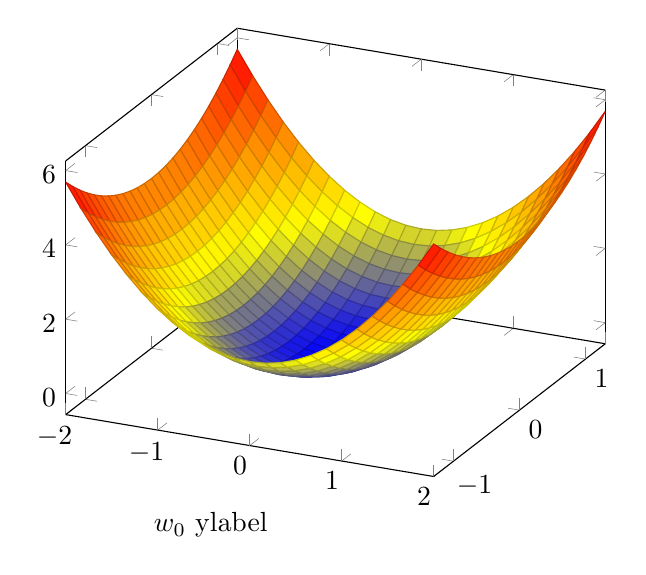
\begin{tikzpicture}
 
  \begin{axis}[
  xlabel = $w_0$
  ylabel = $w_1$
  ]
   
    \addplot3[
	surf,
	domain=-2:2,
	domain y=-1.3:1.3,
] 
	{x^2+y^2};

    
  \end{axis}
\end{tikzpicture}
\caption{The cost landscape of a bivariate function}
\label{fig:costscape}
\end{center}
\end{figure}

To make things simple, lets assume our network only has two weights, though the following derivation generalises to any number of weights. This could give us a cost landscape like that shown in \autoref{fig:costscape}. Our aim is to minimise the cost as the cost is a measure of how wrong our network is.

In more definate terms we wish to minimise \autoref{eqn:cost_bivar}, where $Y_i$ is the desired output value for input $i$ and $z$ is as defined in \autoref{eqn:z_act}.

\begin{equation}
C(w_0, w_1) = \frac{1}{n}\sum_{i=0}^{n} (Y_i - \sigma(z_i))^2
\label{eqn:cost_bivar}
\end{equation}

This is the mean squared error rewritten slightly to highlight the dependence on the weights of the network.

If we make a small change to either of the weights $w_0$ and $w_1$ we will get a small change in the cost, $C$ as seen in \autoref{eqn:delta_C}.

\begin{equation}
\Delta C \approx \frac{\delta C}{\delta w_0} \Delta w_0 + \frac{\delta C}{\delta w_1} \Delta w_1
\label{eqn:delta_C}
\end{equation}

We want to minimise C so we want $\Delta C$ to be negative. To make $\Delta C$ negative we will need to first denote that the gradient of $C$, $\nabla C$. 

\begin{equation}
\nabla C \equiv (\frac{\delta C}{\delta w_0}, \frac{\delta C}{\delta w_1})^T
\label{eqn:nabla_c}
\end{equation}

In \autoref{eqn:nabla_c} we can see that the gradient of $C$ is equivalent to the partial derivatives of $C$ with repect to the weights of the network. For simplicity we will collect the changes in weights into a single vector $\Delta w \equiv (\Delta w_0, \Delta w_1)^T$.

By substituing this into \autoref{eqn:delta_C} we get \autoref{eqn:delta_c_sub}.

\begin{equation}
\Delta C \approx \nabla C \cdot \Delta w 
\label{eqn:delta_c_sub}
\end{equation}

Looking at \autoref{eqn:delta_c_sub}, we can see that to make $\Delta C$ negative we can set $\Delta w$ as in \autoref{eqn:delta_w_eta}, where $\eta$ is a small positive constant called the learning rate.

\begin{equation}
\Delta w = -\eta \nabla C
\label{eqn:delta_w_eta}
\end{equation}

By substituting \autoref{eqn:delta_w_eta} into \autoref{eqn:delta_c_sub} we can see that $ \Delta C = - \eta \abs{\nabla C}^2$ and because
 $\abs{\nabla C}^2 \geq 0$ this gaurantees that $C$ will always decrease if the weights are changed in accordance to \autoref{eqn:delta_w_eta}.

By iteratively making changes to the weights according to \autoref{eqn:delta_w_eta} we will eventually reach the minima of $C$ so long as we select an appropriate learning rate \footnote{Learning rate is discussed in more detail in \autoref{sec:lr_sch}}. 

\subsection{Backpropagation}
With a gradient descent providing a method for adjusting  weights, we now only need one more ingredient to be able to train our neural networks. Whilst our cost function tells us about the error of our network at its output, we need a method to calculate the error for any neuron in any layer - this is exactly what backpropagation does.

Backpropogation is defined by four equations:
1)An equation for the error in the output layer, $\delta_L$:

\begin{equation}
\delta_L = \nabla_a C \circ \sigma'(z_L)
\label{eqn:BP1}
\end{equation}

\autoref{eqn:BP1} shows the output error $\delta_L$ equates to changes in the cost $C$ with respect to its activations $a$ and the derivative of the output layers activation function $\sigma'$ when the input to that layer is $z_L$.

2)An equation for the error $\delta_l$ in terms of the error in the next layer:
\begin{equation}
\delta_l = ((w_{(l+1)})^T\delta_{(l+1)} \circ \sigma'(z_l)
\label{eqn:BP2}
\end{equation}
where $(w_{(l+1)})^T$ is the transpose of the weight matrix for the layer above. Multiplying the error from the layer above by the transposed weight matrix can be seen as moving the error backward through that weight matix and the Hadamard product\footnote{The Hadamard product is the elementwise product of two matricies as shown in \autoref{eqn:hada}. \begin{equation}
\begin{bmatrix}
a & b \\
c & d
\end{bmatrix} \circ \begin{bmatrix}
e & f \\
g & h
\end{bmatrix} = \begin{bmatrix}
ae & bf \\
cg & dh
\end{bmatrix}
\label{eqn:hada}
\end{equation}} $\circ$ with $\sigma'(z_l)$ moves the error backward through the activation function.

3)An equation for the rate of change of the cost with respect to any bias in the network:
\begin{equation}
\frac{\delta C}{\delta b_lj} = \delta_lj
\label{eqn:BP3}
\end{equation}
where $\frac{\delta C}{\delta b_lj}$ is the rate of change of the cost $C$ with respect to bias $b$ of neuron $j$, in layer $l$ and $\delta_lj$ is the $j^{th}$ entry in the error matrix $\delta$ for layer $l$ i.e. the error for the $j^th$ neuron in layer $l$.

4)An equation for the rate of change of the cost with respect to any weight in the network:
\begin{equation}
\frac{\delta C}{\delta w_{ljk}} = a_{(l-1)k}\delta_lj
\label{eqn:BP4}
\end{equation}
where $\frac{\delta C}{\delta w_{ljk}}$ is the rate of change of cost $C$ with respect to the change in weight $w_k$ of neuron $j$ in layer $l$ and $a_{(l-1)k}$ is its input activation.

Using these four \autoref{eqn:BP1}, \autoref{eqn:BP2}, \autoref{eqn:BP3} and \autoref{eqn:BP4}, we can calculate the change in error due to any weight or bias in the network and thus can use gradient descent to optimise its value to reduce the error at the output of the network.

One consequence of the backpropagation algorithm is that we are limited in terms of the trainable depth of our networks. As we continually differentiate the error to pass it back through each layer and multiply it by transposed weight matricies, the magnitude of the error can shrink. This results in vanishing error gradients the deeper into the network we go. This mean that at some point, the error with respect to a weight or bias will appear to be zero (or approxiamtely zero) and thus we cannot adjust it by gradient descent, so we are limited to not having infinitely deep networks.

\subsection{Extensions and Improvements}
There are many extensions to simple gradient descent based learning, here are a few to be aware of.
\subsubsection{Learning Rate Schedule}
\label{sec:lr_sch}
Depending on how far we are from the global error minima, we may wish to change the value of the learning rate $\eta$. Recall from \autoref{eqn:delta_w_eta} $\Delta w = -\eta \nabla C$, that the learning rate determines how big of a step we take, following the gradient of the error, each time we update the weights of our neural network.

If we are far from the minimum point for the cost with respect to the weights, we may wish to take larger steps, so that we can more quickly reduce the total cost. However, as we get closer we want to ensure that we do not step over the minimum.

\begin{figure}[h]
\begin{center}
\begin{tikzpicture}
\begin{axis}[
axis lines=left,
xtick={-10,0,10},
xticklabels={},
xlabel={$\Delta w$},
ylabel={$C$},
yticklabels={},
xlabel near ticks,
ylabel near ticks]
\addplot[black, thick, smooth, samples=1000, domain=-10:10]{x^2};
%\draw [blue](0,100) ++(90 : 1 ) arc ( 90:81.87:50 );
\node [blue] at (2,98)  (a) {\textbullet};
\node [blue] at (20,64) (b) {\textbullet};
\node [blue] at (40,36) (c) {\textbullet};
\node [blue] at (60,16) (d) {\textbullet};
\node [blue] at (80,4)  (e) {\textbullet};
\node [blue] at (100,0) (f) {\textbullet};

\draw[blue, ->](a) to [bend left] (b);
\draw[blue, ->](b) to [bend left] (c);
\draw[blue, ->](c) to [bend left] (d);
\draw[blue, ->](d) to [bend left] (e);
\draw[blue, ->](e) to [bend left] (f);


\node [red] at (198,98)  (g) {\textbullet};
\node [red] at (180,64) (h) {\textbullet};
\node [red] at (153,28) (i) {\textbullet};
\node [red] at (90,1) (j) {\textbullet};
%\node [red] at (60,16)  (k) {\textbullet};
%\node [red] at (80,4) (l) {x};


\draw[red, ->](g) to [bend right] (h);
\draw[red, ->](h) to [bend right] (i);
\draw[red, ->](i) to [bend right] (j);
%\draw[red, ->](j) to [bend right] (k);


\end{axis}
    

\end{tikzpicture}
\caption{Visualisation of cost minimisation in two dimensions for different learning rate schedules. Blue: decreaseing learning rate, Red: large fixed learning rate.}
\label{fig:lr_schedule}
\end{center}
\end{figure}

\autoref{fig:lr_schedule} shows how changing the learning rate schedule can affect how the gradient descent optimiser navigates the cost landscape. The blue arrows show how reducing the learning rate as more training occurs, allows us to not miss the cost minimum. The red arrows show what can happen if we select a large learning rate and don't change it. Whilst at first, we make rapid progress towards the minimum, at somepoint we cross over it and will be unable to approach any closer without taking smaller steps.

This demonstrates nicely why we either select a small learning rate or make use of a learning rate scheduler.
Learning rate schedulers can speed up convergence by allowing large steps to be taken when we are far from the cost minimum with respect to the weights, covering a large distance in a few updates and then slowing down to take smaller steps as we get closer. 

This begs the question of: how do we know when to change the learning rate? in  practice there are many ways we can achieve this, however these braodly fit into two categories, mathematical and heuristic.

There are many algorithms for calculating how to set the learning rate for example, Adam \cite{kingma2014adam} and ADADelta \cite{zeiler2012adadelta}. They are both popular as they are both first order methods, meaning that expensive, slow calculations of second order derivatives do not need to be made.
Senior et al.\cite{senior2013empirical} provide an extensive testing of different learning rate schedulers. 

Second order methods are desirable in that the second derivative of the cost provides information about how the cost gradient is changing. \autoref{fig:2ndordr} shows how the cost and its first and second derivatives change with respect to the weights. In region (A), where the cost (black line) is far from the minima the first derivative (blue) changes rapidly, causing the second derivative (red) to have a large magnitude. In region (B), the cost is closer to the minima, and thus the change in cost is lower so the steepness of the first derivative (blue) is lower as is the magnitude of the second derivative (red). At the minima, the second derivative is exactly zero, so we know we have reached the minima if the second derivative equals zero.

Second order methods have the major draw back of being very slow to calculate. Thus it is more efficient to make use of first order estimates than the exact information provided by second order methods. Many more weight updates can be carried out using first order methods than can be done using second order methods in a given time frame. So whilst second order methods should require less total weight updates to minimise the cost, the first order methods will reach the minimum faster as the weight updates will occur much more quickly in the first order case.


\begin{figure}[h]
\begin{center}
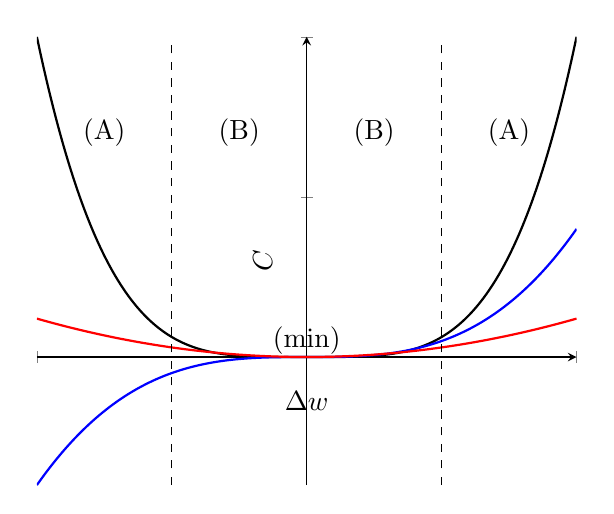
\begin{tikzpicture}
\begin{axis}[
axis lines=middle,
xtick={-10,0,10},
xticklabels={},
xlabel={$\Delta w$},
ylabel={$C$},
yticklabels={},
xlabel near ticks,
ylabel near ticks,
scaled y ticks = false]
\addplot[black, thick, smooth, samples=1000, domain=-10:10]{x^4};
\addplot[blue, thick, smooth, samples=1000, domain=-10:10]{4*x^3};
\addplot[red, thick, smooth, samples=1000, domain=-10:10]{12*x^2};

\addplot [black, thin, dashed] coordinates {(-5, -4000) (-5, 10000)};
\addplot [black, thin, dashed] coordinates {(5, -4000) (5, 10000)};

\node[] at (axis cs:7.5,7000) {(A)};
\node[] at (axis cs:-7.5,7000) {(A)};
\node[] at (axis cs:2.5,7000)  {(B)};
\node[] at (axis cs:-2.5,7000) {(B)};
\node[] at (axis cs:0,500) {(min)};



\end{axis}
    

\end{tikzpicture}
\caption{Visualisation of the cost (black), its first derivative (blue) and second derivative (red).}
\label{fig:2ndordr}
\end{center}
\end{figure}

Heuristic methods provide a very simple method for adjusting the learning rate. A commonly used one is to simply gradually reduce the learning rate by a small amount each epoch. This has the advantage of requiring almost no computational overhead and being very easy to understand. When training starts, we expect performance to be poor, so improvements can be made rapidly. As training progresses, we expect that improvements will be slower as we are approaching the minimum cost.

\section{Convolutional Neural Networks}
\subsection{What is Convolution?}
\subsubsection{Kernels}
\subsubsection{Strides}
\subsubsection{Dilations}
\subsection{Transposed Convolutions}


\section{Recurrent Neural Networks}
\subsection{Vanilla RNN}
\subsection{Gated RNN}

\begin{figure}
	\centering
	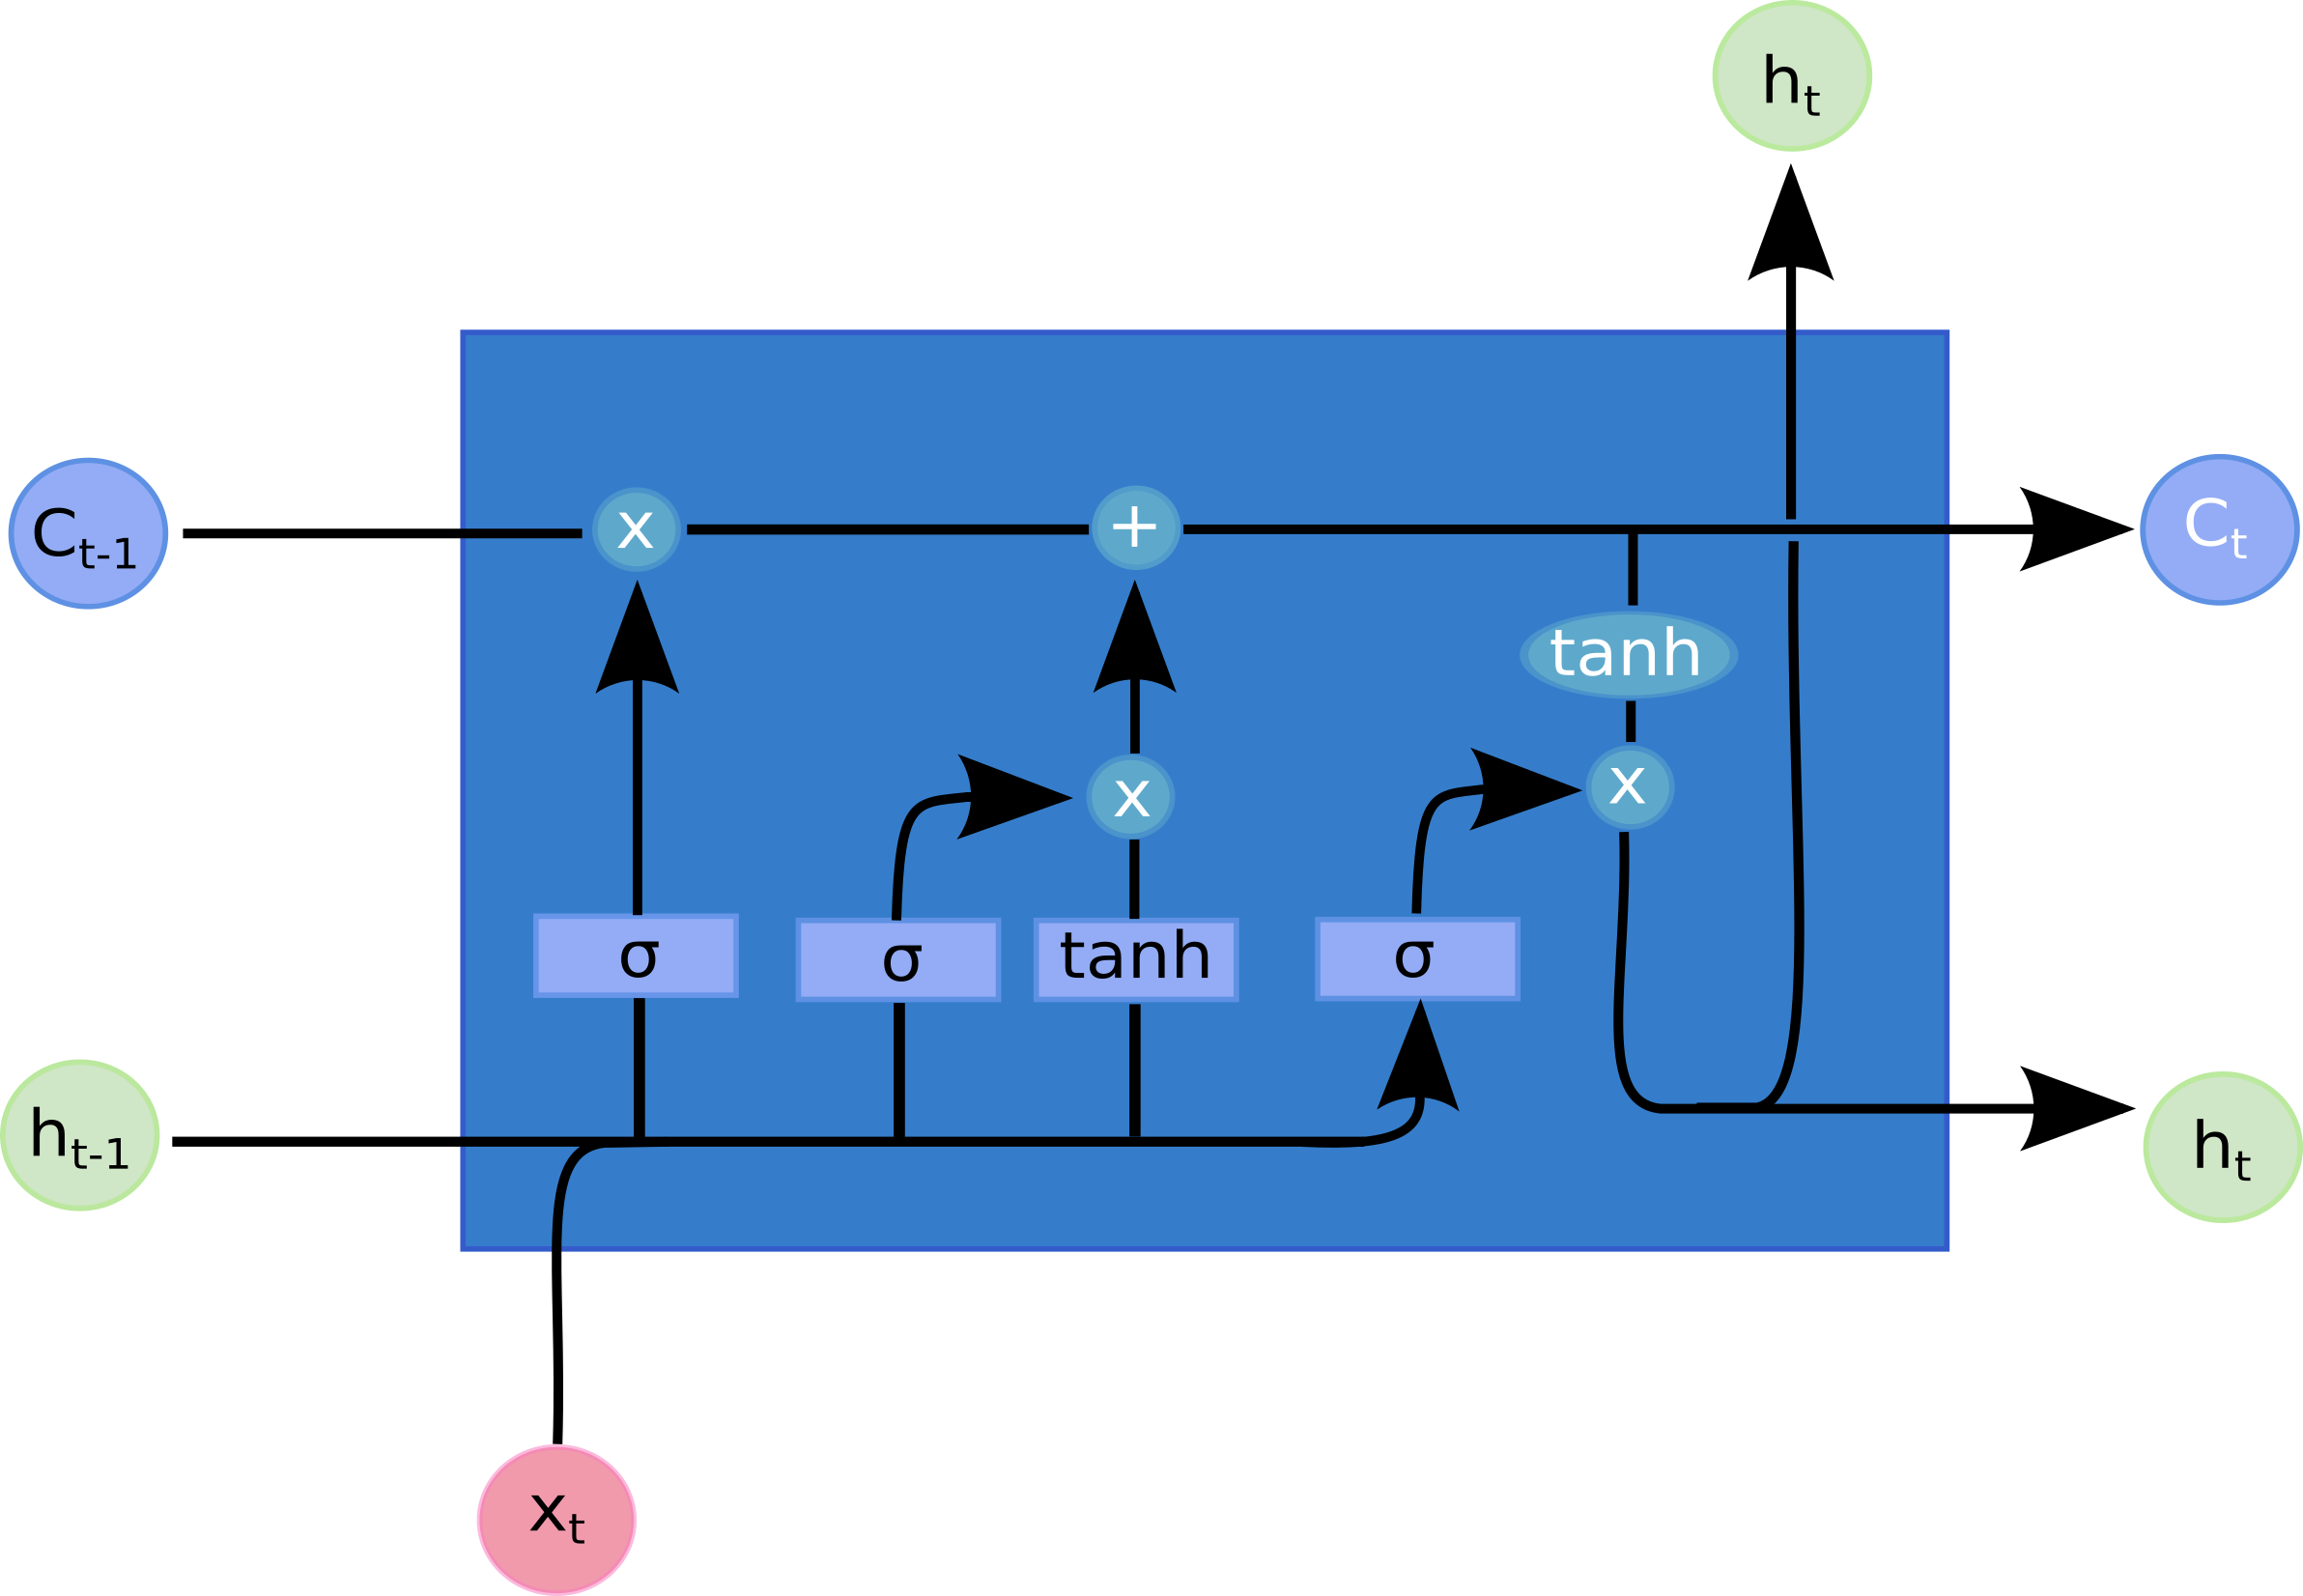
\includegraphics[width=0.5\textwidth]{Figs/intro2dl/LSTM.png}
	
	\caption{A Long Short-Term Memory Unit}
	\label{fig:lstm}
\end{figure}

\begin{figure}
	\centering
	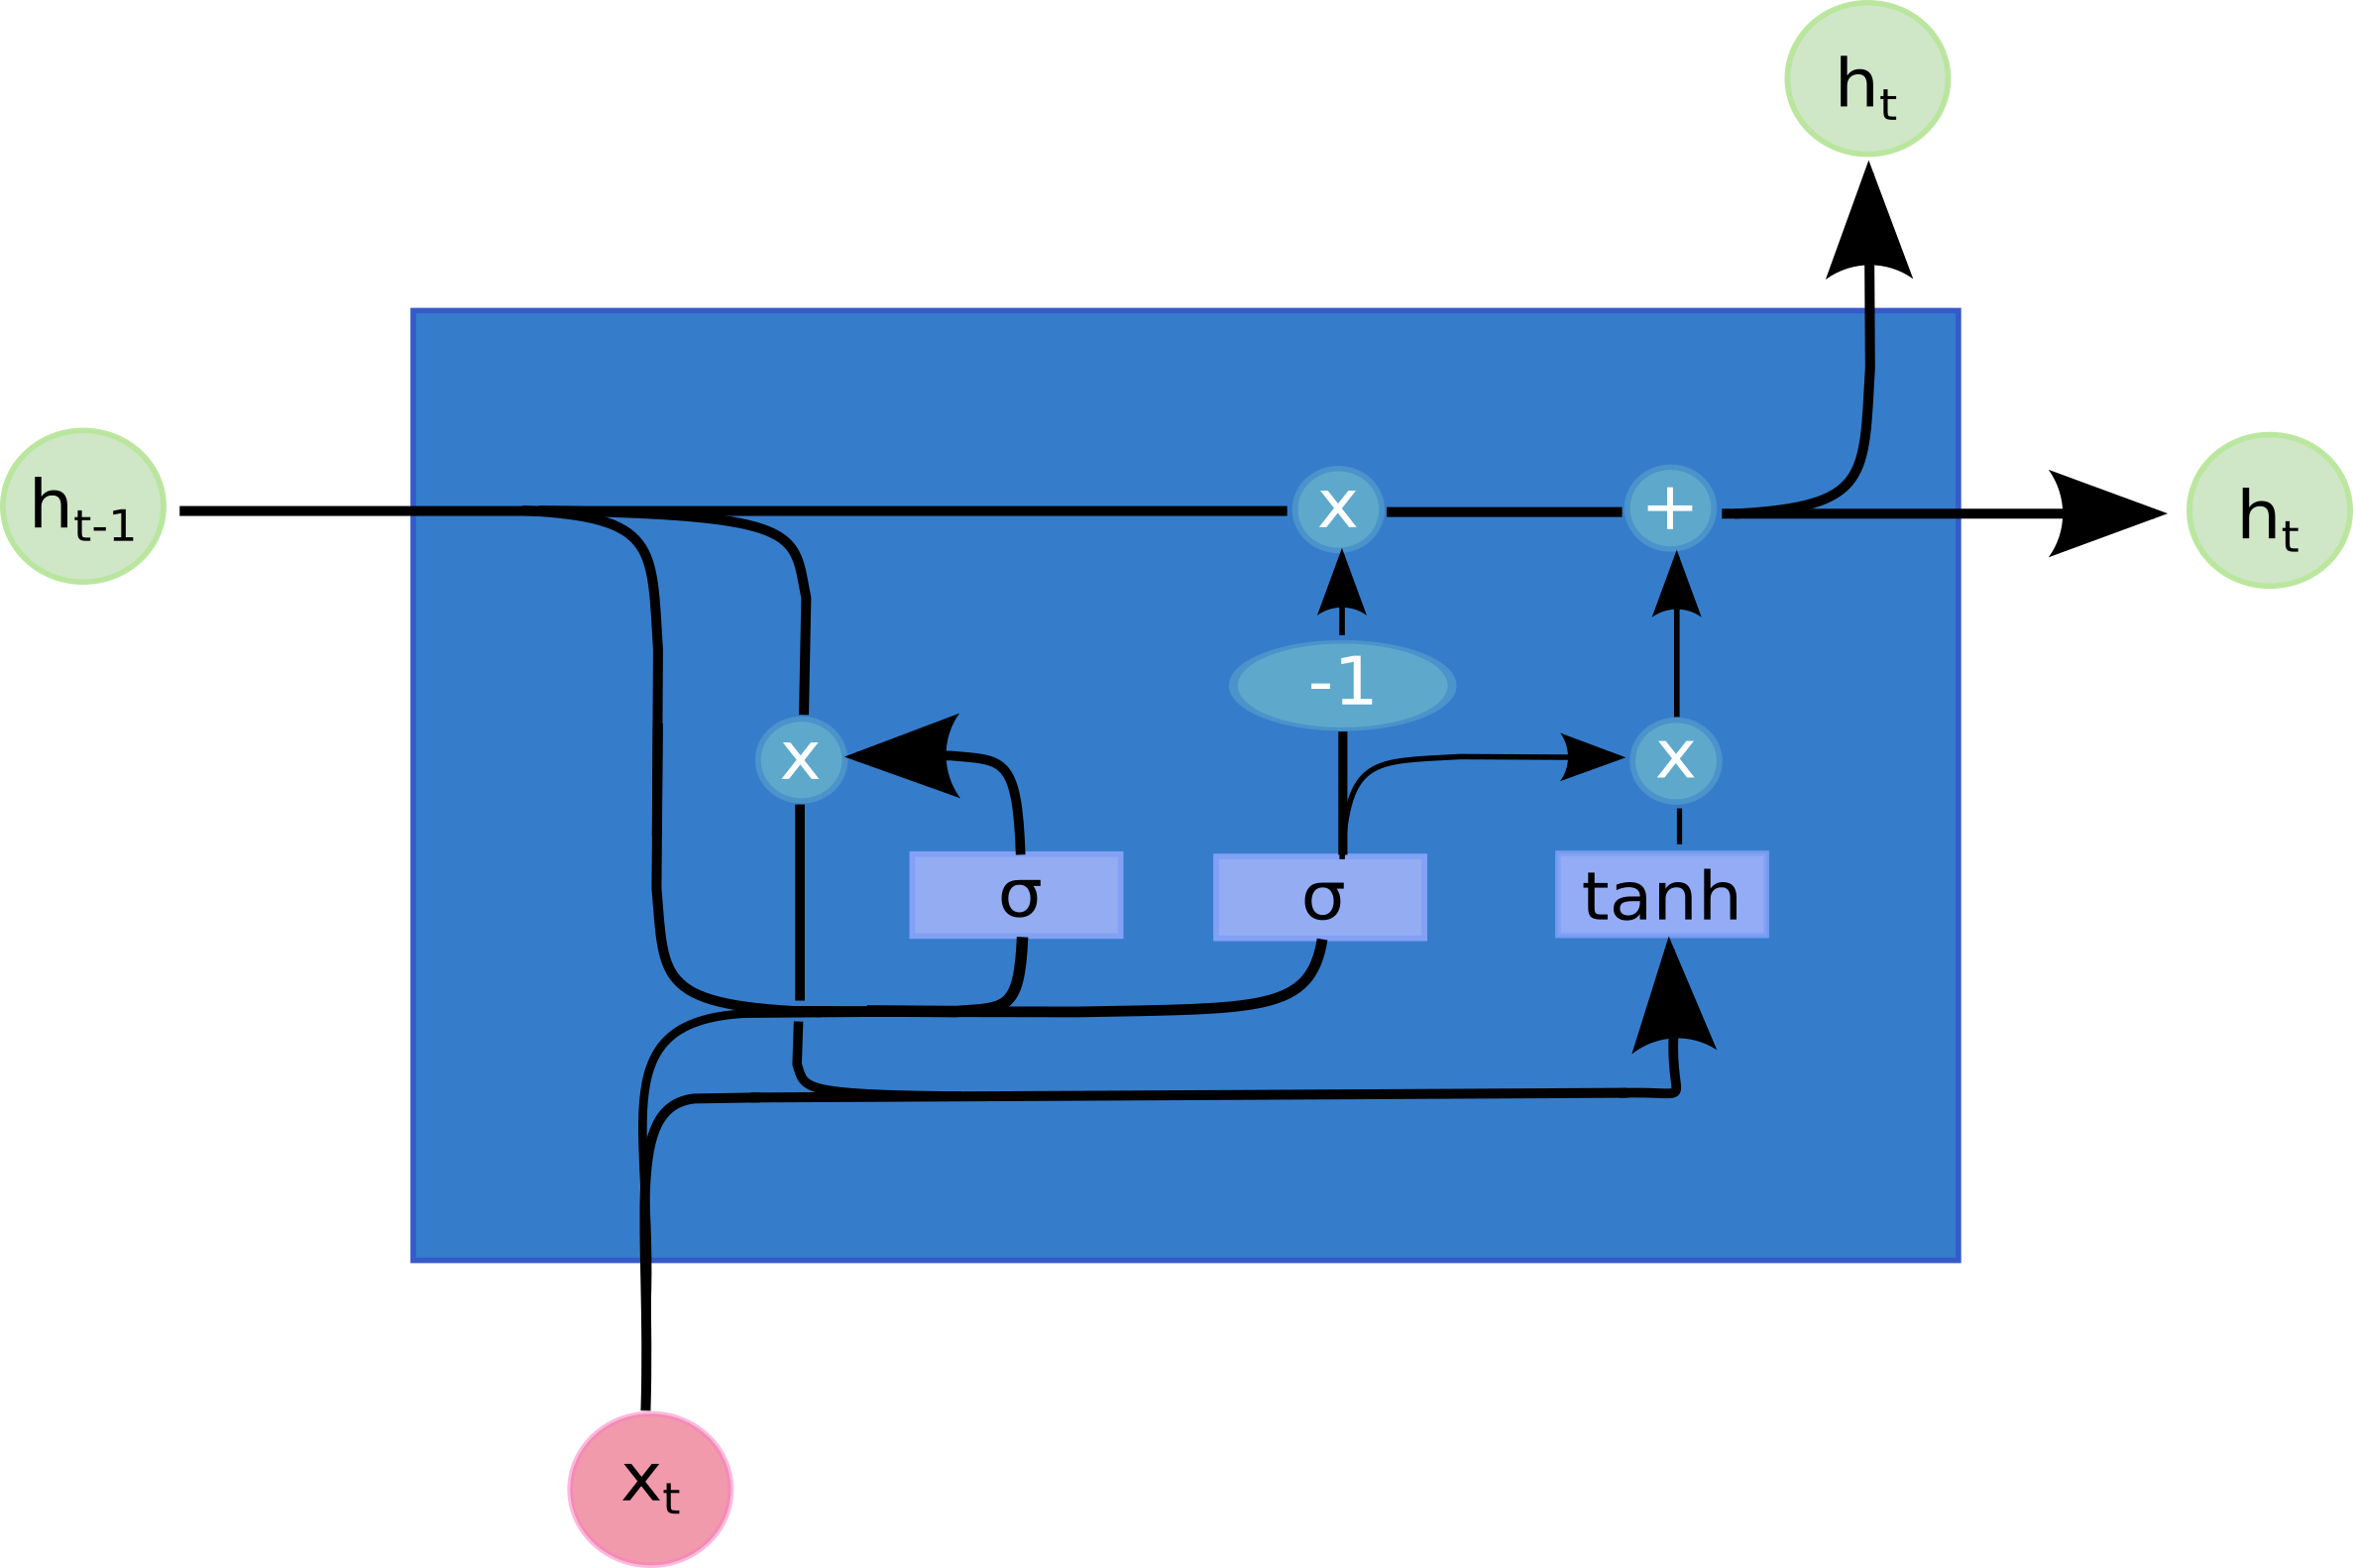
\includegraphics[width=0.5\textwidth]{Figs/intro2dl/GRU.png}
	
	\caption{A Gated Recurrent Unit}
	\label{fig:gru}
\end{figure}



\section{Summary}
 
 
% Chapter Template

\chapter{Sensory Redundancy: Are Two Heads Better Than One?} % Main chapter title

\label{Chapter4} % Change X to a consecutive number; for referencing this chapter elsewhere, use \ref{ChapterX}

\lhead{Chapter 4. \emph{Sensory Redundancy: Are Two Heads Better Than One?}} % Change X to a consecutive number; this is for the header on each page - perhaps a shortened title

%----------------------------------------------------------------------------------------
%	SECTION 1
%----------------------------------------------------------------------------------------

\section{Why Have One Sensor When Two Are Better?}
A key part of the human experience is that it is multisensory. In \cite{barsalou2008grounded}, Lawrence Barsalou speaks about how multisensory processing aids human cognition in a number of ways. Firstly, multisensory information aids in the classification of experiences by providing additional and complimentary information that is not accounted for in only a single modality. 

Lip reading affects the classification of phonemes, this is known as the Mcgurk effect \cite{mcgurk1976hearing}. Whilst this effect can lead to incorrect classifications when misaligned data is provided e.g. utterances of the syllable [ba] dubbed on to lip movements for [ga], lead to normal adults hearing [da]; in normal circumstances, like when two people are speaking to one and other, lip reading aids in classifying heard sounds \cite{ma2009lip}. This is particularly important in noisy environments, which leads to another of Barsalou's ideas about multisensory processing: information redundancy.

The reason that lip reading can aid hearing in noisy evironments is that it provides an additional vector along which the human brain can reconstruct missing information. When something is mis-heard due to background noise, the visual information gained from looking at the lips of the speaker can be used to reconstruct their utterance.

The ability to reconstruct missing data from a secondary modality has not only been seen in humans \cite{ma2009lip, samuel1997lexical} but has been demonstrated in computational modals for example,\cite{ngiam2011multimodal, silberer2014learning}.

In order to be able to reconstruct missing data from a secondary modality, symbol grounding needs to have occured, and the meaning of a percept in modality A must be known in modality B.
If both the forward and inverse relationship between modalities is known, then bidirectional symbol grounding has occured and we are able to reconstruct modality A from modality B and modality B from modality A.

In this chapter I will explore these two ideas, improved classification and reconstruction of missing information through  bidirectional symbol grounding using \acp{MAE}.



\section{Generating Images From Natural Language}
\subsection{Aims}
The experiment in this section demonstrates that having access to a second modality improves classification accuracy over the baseline accuracy of classification of either of the two individual modalities as well as how missing data can be reconstructed from a secondary modality.

\subsection{A note on Qualatitive Anaylsis of Image Generation}
\textcolor{red}{As quantitive analysis of generated images is difficult. I will make use of a qualititive analysis to describe the quality of the images generated in this and subsequent chapters.
This is in line with the the analysis performed in \cite{reed2016generative, zhang2017stackgan, xu2018attngan, li2018video, mansimov2015generating} in which human analysis of generated images is used.}

\textcolor{red}{However \cite{zhang2017stackgan, xu2018attngan, li2018video} also make use of Inception score to provide a quantitive measure of the images they generate. Inception score is the \ac{KLD} between $P(y|x)$ and $P(y)$ where $x$ is a generated image and $y$ is a class label generated by a pretrained classifier (\cite{zhang2017stackgan, xu2018attngan, li2018video} make use of the Inception net \cite{szegedy2017inception} for this classification, hence the name of their metric.}

\textcolor{red}{Inception score is not suitable for my purposes for two main reasons. 1) I do not have pretrained classifiers for the datasets used in this thesis and 2) Inception score only indicates whether a generated image can be classified into a particular category, it does not indicated whether the image matches the description from which it was generated as noted by Zhang et al in \cite{zhang2017stackgan}.}

\begin{displayquote}
Although the inception score has shown to well correlate
with human perception on visual quality of samples, it
cannot reflect whether the generated images are well con-
ditioned on the given text descriptions.
- Zhang et al.
\end{displayquote}

In order to make the qualititive analysis of generated images more precise, a list of the adjectives I use and the visual properties to which they relate can be seen in \autoref{tab:adjs}. 

\begin{table}
		\centering
		\begin{tabular}{|c|c|}
			\hline
			\textbf{Adjective} & \textbf{Property} \\ \hline
		Prototypical & whether an image is a typical represention of the categroy to which it belongs.

		\end{tabular}
		\caption{Adjectives used for the qualititive analysis of generated images.}
		\label{tab:adjs}
	\end{table}


\subsection{UCU Arabic Spoken Digits and MNIST} 
\label{sec:UCU}
This experiment utilises two datasets, UCU Arabic Spoken Digits (UCU) and MNIST Handwritten Digits (MNIST).

\subsubsection{UCU Arabic Spoken Digits}
UCU is a dataset containing the 13 \acp{MFCC} representing the audio of the digits 0 to 9 being said by 88 different speakers \cite{hammami2009tree,hammami2010improved}. It contains 8800 utterances (10 digits x 10 repetitions x 88 speakers). Audio was sampled at 11025Hz.

\paragraph{Padding of Utterances}
As utterances are not of a fixed length, it is necessary to pad the utterances to be equal length. The longest utterance in the dataset contains 93 samples. For ease of up and downsampling within the neural network, all uttereances are padded to be 100 samples long by appending zeros. Each sample is also padded to contain 16 features, the 13 \acp{MFCC} and 3 zeros to further facilitate up and down sampling\endnote{Up and down sampling is easier with even numbers of features and samples as we can half the size of the data using strided convolutions, s=(2,2), without worrying about integer division errors e.g. $5/2=2$ but $2\times2 \neq5$}.

As I will be classifying the digits, it is necessary to check that padding the digits does not provide a cheat for this. As such, I analyse the mean number of samples for each digit and their standard deviations as depicted in \autoref{fig:ucu_dig_length}. I then perform a linear regression on the number of samples to demonstrate that it is not possible to accurately predict a digit's class given only the length of the utterance.

\begin{figure}
\centering
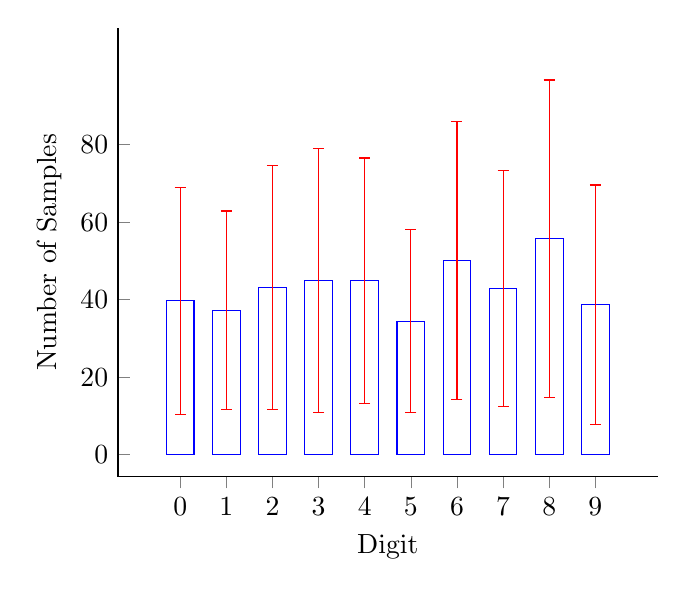
\begin{tikzpicture}
\begin{axis}[
	axis x line*=bottom,
	axis y line*=left,
	%at={(-1,0)}
    ybar,
    enlargelimits=0.15,
    ylabel={Number  of Samples},
    ytick={0,20,40,60,80},   
    xtick={1,2,3,4,5,6,7,8,9,10},
    xticklabels={0,1,2,3,4,5,6,7,8,9}, %{zero, one, two, three, four, five, six, seven, eight, nine}
    %x tick label style={rotate=45},
    xlabel={Digit},
    %nodes near coords,
    %nodes near coords align={vertical},
    xlabel near ticks,
	ylabel near ticks,
	bar shift=0pt
    ]
%\addplot coordinates {(1,39.66) (2,37.27) (3,43.11) (4,45.02) (5,44.92) (6,34.44) (7,50.10) (8,42.81) (9,55.67) (10,38.63)};
\addplot[blue, error bars, y dir=both,y explicit, error bar style={color=red}]
 coordinates { 
(1,39.66) +- (0.0,29.25) 
(2,37.27) +- (0.0,25.58) 
(3,43.11) +- (0.0,31.43) 
(4,45.02) +- (0.0,34.05) 
(5,44.92) +- (0.0,31.63) 
(6,34.44) +- (0.0,23.63)
(7,50.10) +- (0.0,35.90)
(8,42.81) +- (0.0,30.41)
(9,55.67) +- (0.0,41.01)
(10,38.63) +- (0.0,30.94)
  };
\end{axis}
\end{tikzpicture}

	%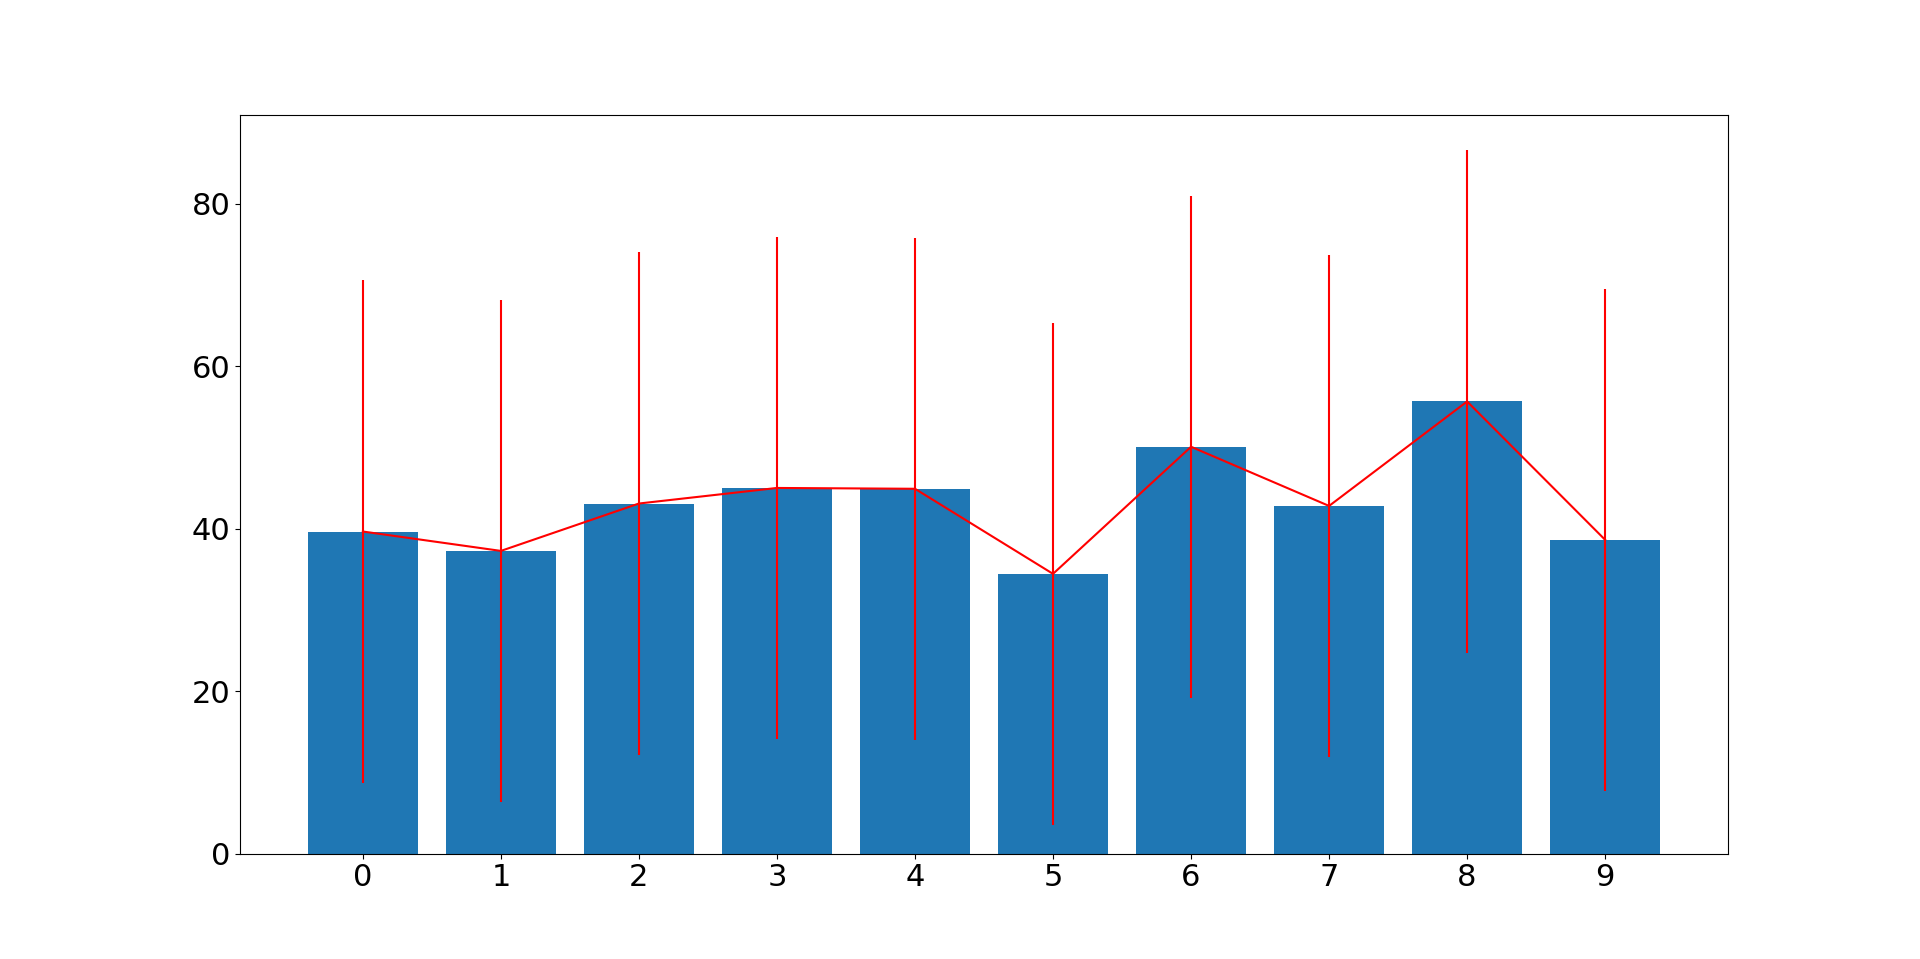
\includegraphics[width=\textwidth]{./Figs/mnistSpoken/UCU_digit_length.png}
	\caption{Mean number of samples for each digit in the UCU Arabic Spoken Digits Dataset. Red bars show the standard devaition in length for each each digit.}
	\label{fig:ucu_dig_length}

\end{figure}

\autoref{fig:ucu_dig_length} shows the mean number of samples for each digit in the UCU dataset. Whilst there is a difference in the mean length of each digit, the standard deviation for each digit is relatively large as can be seen in \autoref{tab:UCU_sampLen}. Therefore, trying to classifiy the digits just by the number of samples in an example, is ineffective.

	\begin{table}
		\centering
		\begin{tabular}{|c|c|c|}
			\hline
			\textbf{Digit} & \textbf{Mean Length (samples)} & \textbf{Standard Deviation} \\ \hline
			0 & 39.66 & $\mypm 29.25$ \\ \hline
			1 & 37.27 & $\mypm 25.58$ \\ \hline
			2 & 43.11 & $\mypm 31.43$ \\ \hline
			3 & 45.02 & $\mypm 34.05$ \\ \hline
			4 & 44.92 & $\mypm 31.63$ \\ \hline
			5 & 34.44 & $\mypm 23.63$ \\ \hline
			6 & 50.10 & $\mypm 35.90$ \\ \hline
			7 & 42.81 & $\mypm 30.41$ \\ \hline
			8 & 55.67 & $\mypm 41.01$ \\ \hline
			9 & 38.63 & $\mypm 30.94$ \\ \hline

		\end{tabular}
		\caption{Mean length and standard deviation of digits in the UCU dataset.}
		\label{tab:UCU_sampLen}
	\end{table}


Performing a linear regression on the number of samples for each digit versus its class, we get an accuracy of 6.18\% when classifying the test set.

\subsubsection{MNIST Handwritten Digits}
MNIST is a well known and oft used dataset in the machine learning community. It contains 60,000 training samples and 10,000 test samples, evenly split between the digits 0 to 9. 
Each digit is presented as a grey-scale, 28x28 pixel image \cite{lecun1998mnist}. 

\subsection{Problem Description}
The experiments with these datasets will explore two problems: classification and bidirectional symbol grounding. 

\subsubsection{Classification}
Each of the utterances and images from the UCU and MNIST datasets are classified as being a numeric digit, 0 to 9. By combining both datasets, I can explore whether the addition of a second modality enhances overall classification accuracy.

I start off exploring the classification abilities of neural networks by performing a linear regression with a single, dense neural network layer with a softmax activation on the activation of the embedding layer of an autoencoder, this is the neural networks representation of the digit. To generate baseline classification accuracies for each dataset, I use autoencoders for each modality separately.

Once a classification baseline has been established for each dataset, I make use of a \ac{MAE}, using paired examples from each dataset to train it.

\subsubsection{Bidirectional Symbol Grounding}

I demonstrate that a neural network can perform bidirectional symbol grounding \cite{barsalou2008grounded} when presented with aligned images and utterances. To explore this, I show how a \ac{MAE} can learn to reconstruct the correct image of a digit given the \acp{MFCC} of an utterance as well as \acp{MFCC} which have a small mean squared error from the correct utterance given an image of a digit. This shows that an internal symbolic language has been learnt in the form of the latent embedding created by the encoders of the \ac{MAE}.


\subsection{Experiment Details}
Images from the MNIST dataset are kept at their original scale of 28x28 pixels and are normalised such that each pixel has a value from 0 to 1 based on its intensity, with zero equating to black and 1 being white.

The UCU dataset is normalised so that all \acp{MFCC} take a value from 0 to 1 based on the value of the \ac{MFCC} such that the highest value is 1 and the lowest 0. Utterances are padded to be 100x16 as previously described.

\paragraph{Combining Datasets}
\label{sec:UCU_mnist_comb}
Due to the difference in size between the datasets, 8,800 samples for UCU and 80,000 samples for MNIST, I randomly sample from the UCU dataset and pair this with a sample from MNIST. This means that each sample from UCU is used approxiamtely 9.1 times ($80000/8800=9.0909$) in the training data.

\paragraph{Merging Modalities}
In order to combine the two different modalities, I explore different merging techniques: concatenation (\textit{Concat}) and addition (\textit{Add}). To do this, the embeddings of both modalities are ensured to have the same shape and then are merged using the methods described in \autoref{eqn:concat} and \autoref{eqn:add} for concatenation and addition, respectively. %and \ref{eqn:xply}.

 \begin{equation}\label{eqn:concat}
 	merged = Im_i^{emb} || MFCC_i^{emb} 	
 \end{equation}

 \begin{equation}\label{eqn:add}  
 	merged = Im_i^{emb} + MFCC_i^{emb} 	
 \end{equation}
 
  %\begin{equation}
 	%merged = x1^*_i * x2^*_i
 	%\label{eqn:xply}  
 %\end{equation}

Where $Im_i^{emb}$ and $MFCC_i^{emb}$ represent the embeddings, output by the image and \ac{MFCC} encoders respectively for image and \ac{MFCC} inputs $Im_i$ and $MFCC_i$.

\subsubsection{Training Procedures}

The \acp{MAE} are trained in two different ways for both types of merging, these are referred to as bimodal (Bi) and randomly removed (RR).

\paragraph{Bimodal}
Under the Bi training procedure, the \ac{MAE} is presented with bimodal input for all training instances. Both image and \ac{MFCC} inputs are present for all training steps and the \ac{MAE} is trained to reproduce this input as its output.

\paragraph{Randomly Removed}
Under the RR training procedure, one third of image inputs are removed at random and one third of \ac{MFCC} inputs are removed at random. It is ensured that each training instance always has at least one input modality present. That is, a training instance never has both its image and \ac{MFCC} input removed. 

The removed modality is replaced with an array of zeros of the same shape as the original input (28x28 for the image and 100x16 for \acp{MFCC}).

The \ac{MAE} is then trained to reproduce both the image and \acp{MFCC} regardless of whether one of these has been ommited from the input.

\subsubsection{Testing Conditions}
Each \ac{MAE} (\textit{Concat} and \textit{Add}) was tested in three different ways, Bimodal, Image Only and \ac{MFCC} Only.

\paragraph{Bimodal}
In the Bimodal testing condition both image and \ac{MFCC} data are used as input for each testing instance and I am interested in observing the classification accuracy as well as the total regeneration error.

\paragraph{Image Only}
In the Image Only testing condition, only images are provided as input data. I am interested in the classification accuracy as well as the \ac{MFCC} reconstruction error. I am not interested in the image reconstruction error, as it is expected that, as the image is provided as input this will be low (which it is for all models and training procedures as seen in \autoref{tab:mnist_ucu_master_res}).  

\paragraph{\ac{MFCC} Only}
Similarly to the Image Only condition, the \ac{MFCC} Only condition provides only \acp{MFCC} as input and I am interested in the classification accuracy as well as the image reconstruction error. I am not interested in the \ac{MFCC} regeneration loss as \acp{MFCC} are given as input it will be low (which it is for all models and training procedures as seen in \autoref{tab:mnist_ucu_master_res}).  

\subsubsection{Network Description}
\paragraph{Baseline Models}
To generate the baseline classification accuracies for both the UCU and MNIST data, I make use of (unimodal) autoencoders. The descrition of the autoencoder for the MNIST dataset can be found in \autoref{tab:MNIST_AE_description} and the autoencoder for the UCU dataset in \autoref{tab:UCU_AE_description}.

	\begin{table}[th!]
		\centering
		\begin{tabular}{|c|c|c|c|c|c|c|}
			\hline
			\textbf{Block} & \textbf{Layer} & \textbf{Type} & \textbf{Neurons} & \textbf{Kernel} & \textbf{Strides} & \textbf{Activation}  \\ \hline
			\multirow{4}{*}{Encoder} & 1	&	2D Conv & 32 & (3,3) & (1,1)  & Relu\\ \cline{2-7}
			& 2	&	2D Conv & 64 & (3,3) & (2,2) & Relu \\ \cline{2-7}
			& 3	&	2D Conv & 64 & (3,3) & (2,2) & Relu \\ \cline{2-7}
			& 4 	&	Dropout p=0.25 &	 & 	     &       & \\ \hline
			Embedding & 5	&	2D Conv & 32 & (3,3) & (1,1) & Relu \\ \hline
			Classifier & 6c	&	Dense          & 10 &       &       & Softmax      \\ \hline
			\multirow{5}{*}{Decoder}& 6 	&	Dropout p=0.25 &	 & 	     &       & \\ \cline{2-7}
			& 7	&	2D Trans Convn & 64 & (3,3) & (2,2) & TanH \\ \cline{2-7}
			& 8	&	2D Transp Conv & 64 & (3,3) & (2,2) & TanH \\ \cline{2-7}
			& 9	&	2D Trans Conv & 32 & (3,3) & (1,1) & TanH \\ \cline{2-7}
			& 10	&	2D Trans Conv & 1 & (3,3) & (1,1) & Sigmoid \\ \hline
		\end{tabular}
		\caption{Image autoencoder and classifier. Layer 6c performs classification, whilst the branch starting at layer 6 regenerates the image.}
		\label{tab:MNIST_AE_description}
	\end{table}

	\begin{table}[h!]
		\centering
		\begin{tabular}{|c|c|c|c|c|c|c|}
			\hline
			\textbf{Block} & \textbf{Layer} & \textbf{Type} & \textbf{Neurons} & \textbf{Kernel} & \textbf{Strides} & \textbf{Activation}  \\ \hline
			\multirow{5}{*}{Encoder} & 1	&	2D Conv & 32 & (3,3) & (1,1)  & Relu\\ \cline{2-7}
			& 2	&	2D Conv & 64 & (3,3) & (2,2)  & Relu\\ \cline{2-7}
			& 3 	&	Dropout p=0.25 &	 & 	     &        & \\ \cline{2-7}
			& 4	&	Dense          & 3136 & 	 &        & \\ \cline{2-7}
			& 5   &	Reshape (7,7,64) &    &     &        & \\ \hline
			Embedding & 6	&	2D Conv & 32 & (3,3) & (1,1)  & Relu  \\ \hline
			Classifier & 7c	&	Dense          & 10 &       &        & Softmax \\ \hline
			\multirow{7}{*}{Decoder} & 7 	&	Dropout p=0.25 &	 & 	     &        & \\ \cline{2-7}
			& 9	&	Dense			& 3200 &     &        & \\ \cline{2-7}
			& 10	&	Reshape (25,4,32) &    &    &        & \\ \cline{2-7}
			& 11	&	2D Trans Conv & 64 & (3,3) & (2,2)  & TanH \\ \cline{2-7}
			& 12	&	2D Trans Conv & 64 & (3,3) & (2,2)  & TanH \\ \cline{2-7}
			& 13	&	2D Trans Conv & 32 & (3,3) & (1,1)  & TanH \\ \cline{2-7}
			& 14	&	2D Trans Conv & 1 & (3,3) & (1,1) & Sigmoid \\ \hline
		\end{tabular}
		\caption{\ac{MFCC} autoencoder and classifier. Layer 7c performs classification, whilst the branch starting at layer 7 regenerates the \acp{MFCC}. The addition of reshape layers is to ensure the final shape of the regenerated \acp{MFCC} matches the target shape whilst the embedding shape matches that of the embedding of the image autoencoder.}
		\label{tab:UCU_AE_description}
	\end{table}

\paragraph{Multimodal Autoencoder}
By combining the two autoencoders described in \autoref{tab:MNIST_AE_description}, and \autoref{tab:UCU_AE_description}, a \ac{MAE} is created. The embeddings from each of the unimodal autoencoders are merged by either, concatenation or addition.

 
	\begin{table}[h!]
		\centering
		\begin{tabular}{|c|c|c|c|c|c|c|}
			\hline
			\textbf{Block} & \textbf{Layer} & \textbf{Type} & \textbf{Neurons} & \textbf{Kernel} & \textbf{Strides} & \textbf{Activation}  \\ \hline
			\multirow{2}{*}{Image} & 1i	&	2D Conv & 32 & (3,3) & (1,1) & Relu \\ \cline{2-7}
			& 2i	&	2D Conv & 64 & (3,3) & (2,2) & Relu \\ \cline{2-7}
			\multirow{2}{*}{Encoder}& 3i	&	2D Conv & 64 & (3,3) & (2,2) & Relu \\ \cline{2-7}
			& 4i	&	Dropout p=0.25 &	 & 	     &       &  \\ \hline

			\multirow{3}{*}{MFCC} & 1m	&	2D Conv & 32 & (3,3) & (1,1) & Relu \\ \cline{2-7}
			& 2m	&	2D Conv & 64 & (3,3) & (2,2) & Relu \\ \cline{2-7}
			& 3m 	&	Dropout p=0.25 &	 & 	     &       & \\ \cline{2-7}
			\multirow{2}{*}{Encoder} & 4m	&	Dense          & 3136 & 	 &       & \\ \cline{2-7}
			& 5m  &	Reshape (7,7,64) & & & & \\ \hline

			Merge & 6im	& Merge & & & & \\ \hline
			Embedding& 7im	&	2D Conv & 32 & (3,3) & (1,1) & Relu \\ \hline
			Classifier & 8c	&	Dense          & 10 &       &       & Softmax \\ \hline

			\multirow{3}{*}{Image} & 8i 	&	Dropout p=0.25 &	 & 	     &       & \\ \cline{2-7}
			& 9i	&	2D Trans Conv & 64 & (3,3) & (2,2)  & TanH \\ \cline{2-7}
			& 10i	&	2D Trans Conv & 64 & (3,3) & (2,2)  & TanH \\ \cline{2-7}
			\multirow{2}{*}{Decoder}& 11i	&	2D Trans Conv & 32 & (3,3) & (1,1)  & TanH \\ \cline{2-7}
			& 12i	&	2D Trans Conv & 3 & (3,3) & (1,1) & Sigmoid\\ \hline 

			\multirow{4}{*}{MFCC} & 8m 	&	Dropout p=0.25 &	 & 	     &        & \\ \cline{2-7}
			& 9m	&	Dense			& 3200 & &           & \\ \cline{2-7}
			& 10m	&	Reshape (25,4,32) & & & &\\ \cline{2-7}
			& 11m	&	2D Trans Conv & 64 & (3,3) & (2,2)  & TanH \\ \cline{2-7}
			\multirow{3}{*}{Decoder}& 12m	&	2D Trans Conv & 64 & (3,3) & (2,2)  & TanH \\ \cline{2-7}
			& 13m	&	2D Trans Conv & 32 & (3,3) & (1,1)  & TanH \\ \cline{2-7}
			& 14m	&	2D Trans Conv & 1 & (3,3) & (1,1)  & Sigmoid\\ \hline
		\end{tabular}
		\caption{Image and MFCC multimodal autoencoder. Layers marked i, m, im and c are image, MFCC, image and MFCC and classification respectively.}
		\label{tab:UCU_MNIST_MAE_description}

	\end{table}


\begin{figure}
\centering
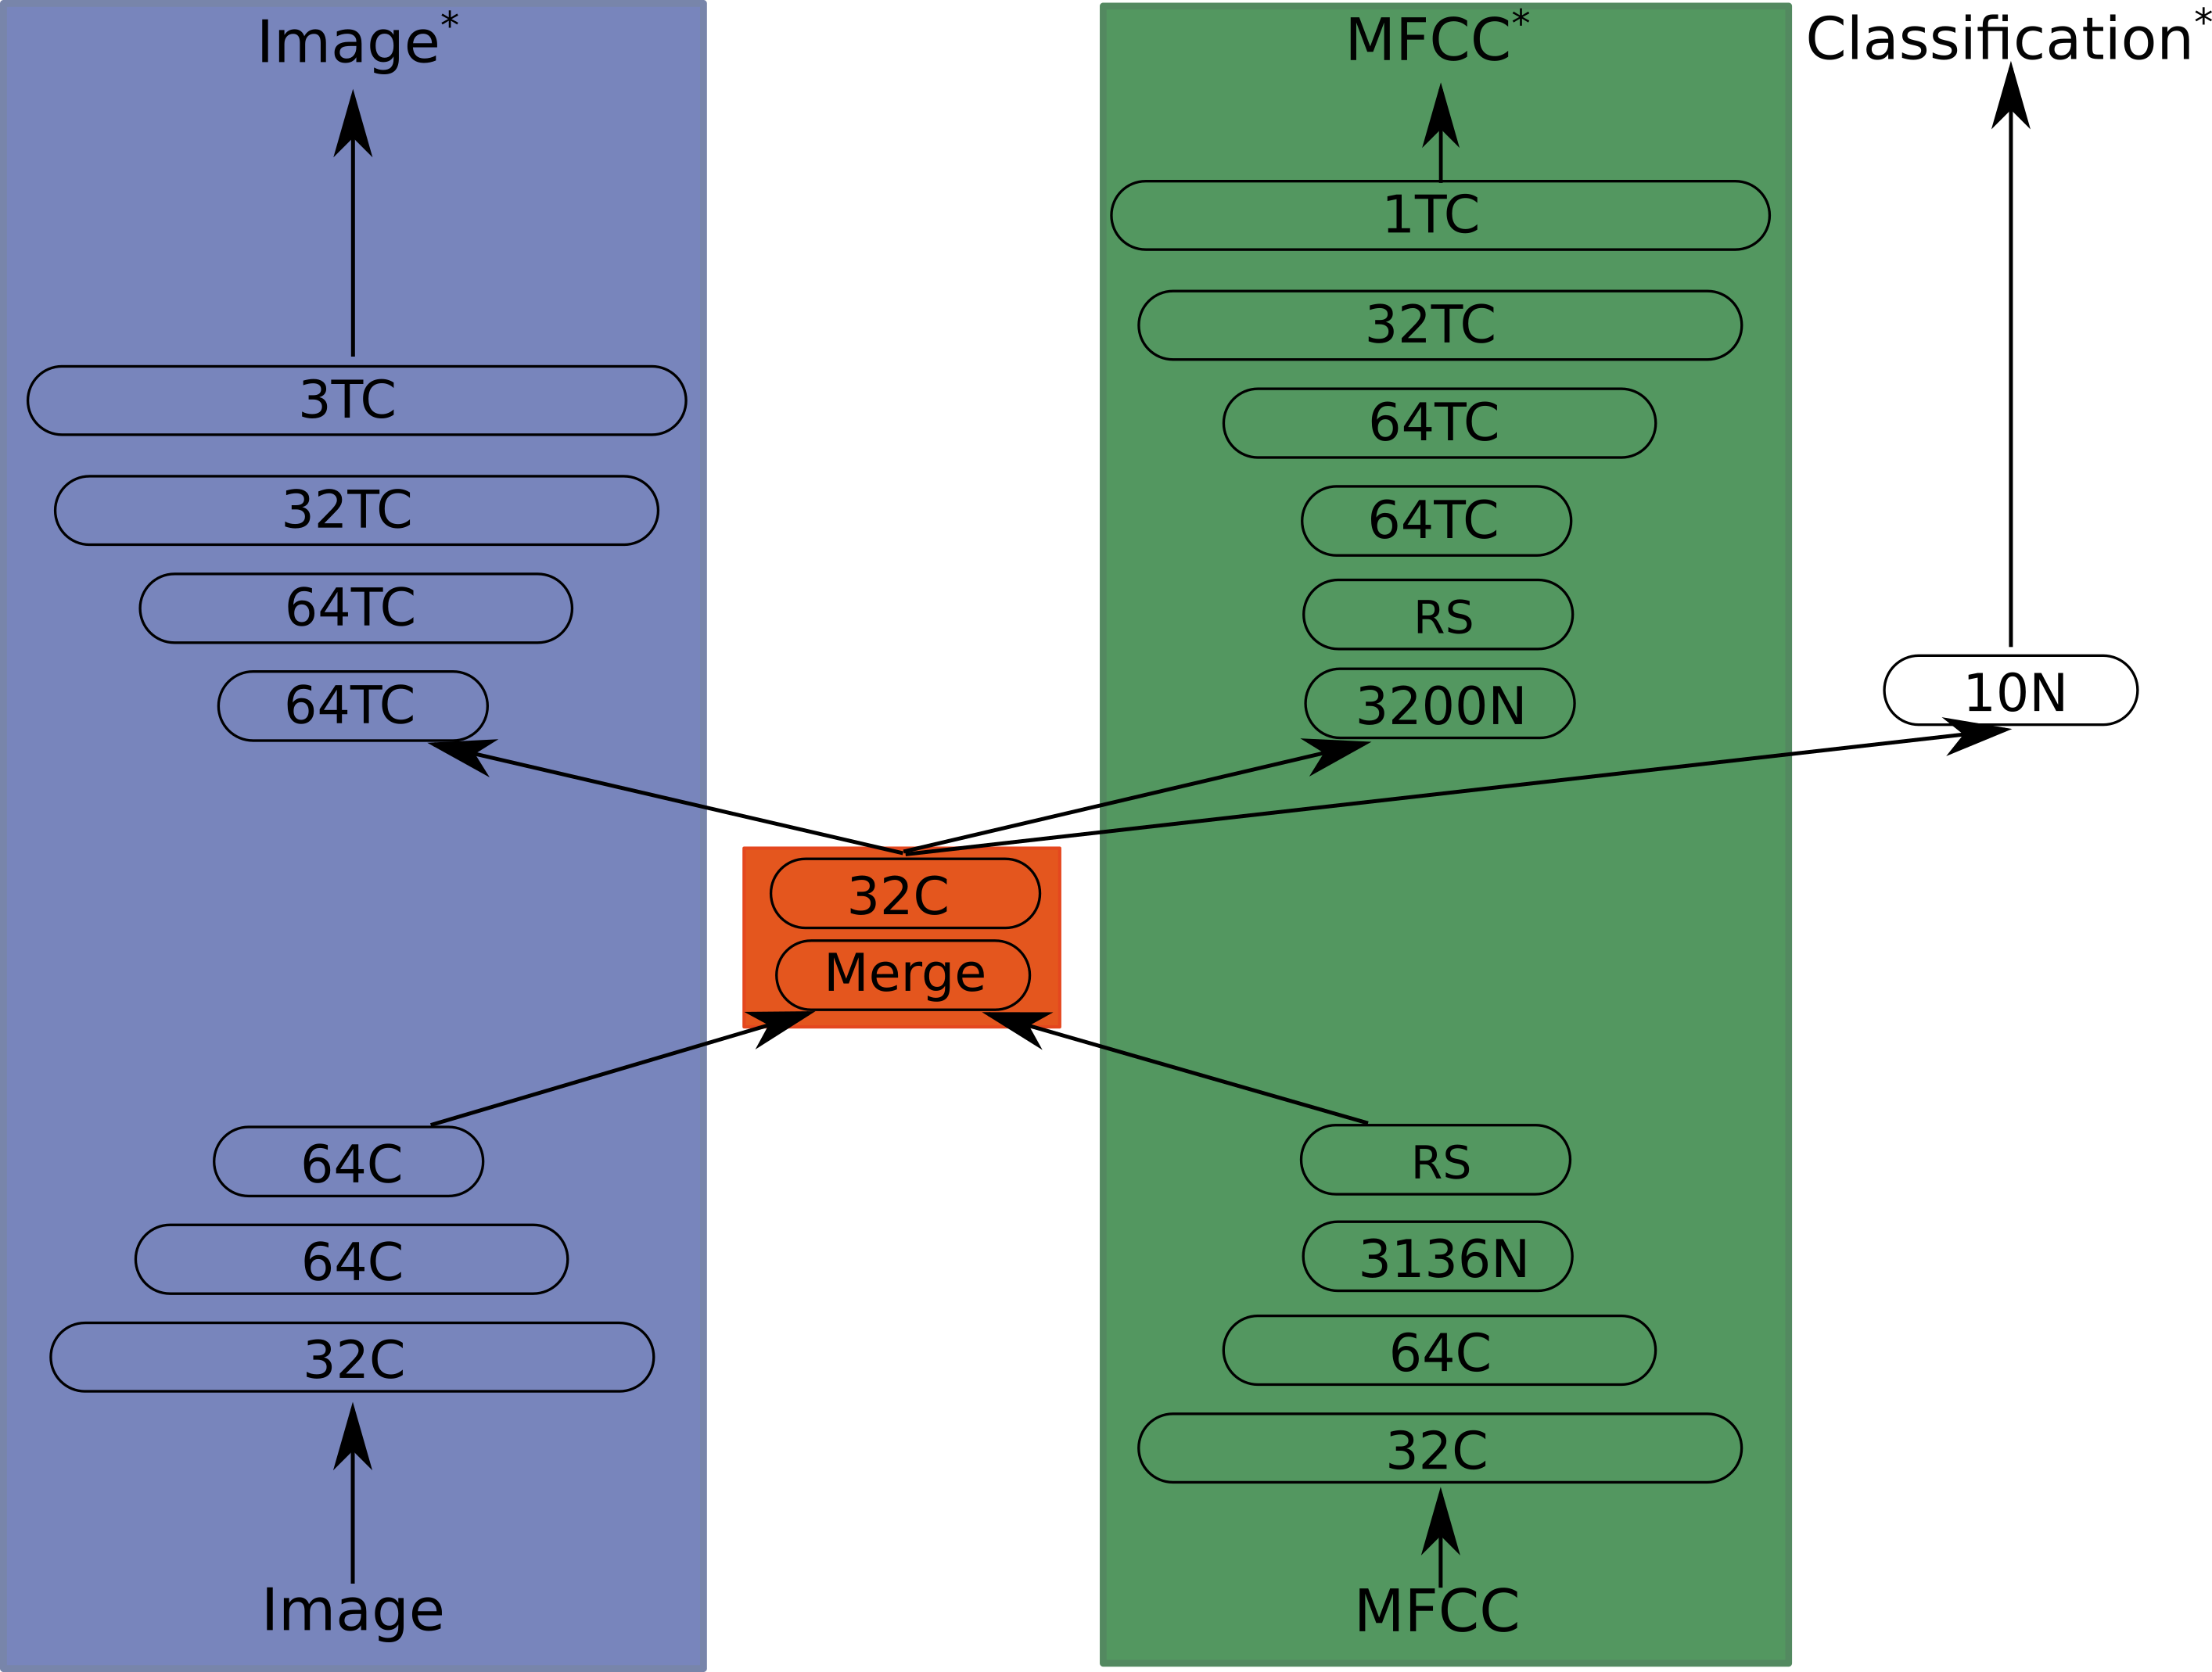
\includegraphics[width=0.75\textwidth]{Figs/mnistSpoken/grounderW2V.png}
\caption{\textcolor{red}{The \ac{MAE} architecture used to bidirectionally ground the MNIST and UCU datasets. Layers marked with C are convolution TC, Transposed Convolution, RS, Reshape and N, Dense.}}
\label{fig:netMnist}
\end{figure}

\textcolor{red}{\autoref{fig:netMnist} depicts the \ac{MAE} described in \autoref{tab:UCU_MNIST_MAE_description}. The blue box shows the portion of the \ac{MAE} which encodes and decodes images, whilst the green portion handles the MFCC data. The orange box is where the joint representation is formed. Inputs are labelled, Image and MFCC with their respective outputs being marked with an asterisk. The final output is the classification which is created by passing the joint representation to a single dense layer containing 10 neurons.}

\subsection{Results}

\subsubsection{Classification Results}
The complete set of results for this experiment are available in \autoref{tab:mnist_ucu_master_res} in \autoref{appendix:app4}. The most important results are shown in the following three tables: \autoref{tab:mnist_ucu_bi_res} for the Bimodal testing condition, \autoref{tab:mnist_ucu_im_res} for the Image Only condition and \autoref{tab:mnist_ucu_mfcc_res} for the \ac{MFCC} Only testing condition. 

All results reported here are the mean of a four-fold cross validation. Each training and testing condition was run four times and the average results are shown.


\begin{table}[h]
	\centering
		\begin{tabular}{|c|c|c|c|c|}
		\hline
		\textbf{Model} & \textbf{Training} & \textbf{Im MSE} & \textbf{MFCC MSE} &  \textbf{Acc} \\ \hline
				Image AE & Im & 	\textbf{0.0027}	&	       			& 	0.9883			\\ \hline		
				MFCC AE & MFCC & 		    		& 	\textbf{0.0113} &	0.9832			\\ \hline		
\multirow{2}{*}{Add MAE} & Bi & 	0.0030			&	0.0401			&	0.9967			\\ \cline{2-5}
						  & RR &	0.0033			&	0.0176			&	\textbf{0.9993}	\\ \hline	
		
\multirow{2}{*}{Concat MAE} & Bi & 0.0031			&	0.0423			&	0.9945			\\ \cline{2-5}		
							 & RR & 0.0030			&	0.0426			&	0.9986			\\ \hline
		\end{tabular}
		\caption{Mean Squared Errors for the Bimodal testing condition, comparing the Bimodal (Bi) and Randomly Removed (RR) training procedures.}
		\label{tab:mnist_ucu_bi_res}

\end{table}

In \autoref{tab:mnist_ucu_bi_res} it can be seen that both concatenate and addition merging produce models with better prediction accuracy than the baseline models, regardless of training procedure.

\begin{table}
	\centering
		\begin{tabular}{|c|c|c|c|}
		\hline
		\textbf{Model} & \textbf{Training} &  \textbf{MFCC MSE} &  \textbf{Acc} \\ \hline
		Image AE & Im 		&  		    			& \textbf{0.9883}	\\ \hline		
\multirow{2}{*}{Add MAE} & Bi & 	0.1641			& 0.4501 			\\ \cline{2-4}
						  & RR & \textbf{0.0455}	& 0.9834 			\\ \hline	
		
\multirow{2}{*}{Concat MAE} & Bi & 	0.2029		&	0.3496 			\\ \cline{2-4}		
							 & RR & 	0.0737		&	0.9834 			\\ \hline
		\end{tabular}
		\caption{Mean Squared Errors for the Image Only testing condition, comparing the Bimodal (Bi) and Randomly Removed (RR) training procedures.}
		\label{tab:mnist_ucu_im_res}

\end{table}

In comparison to the results in \autoref{tab:mnist_ucu_bi_res}, the results in \autoref{tab:mnist_ucu_im_res} show that the \acp{MAE} trained using the Bi training procedure do not generalise well when only a single input modality is available. Whereas the \acp{MAE} trained using the RR training procedure perform almost as well as the baseline model. 
\begin{table}[h]
	\centering
		\begin{tabular}{|c|c|c|c|}
		\hline
		\textbf{Model} & \textbf{Training} & \textbf{Im MSE} &  \textbf{Acc} \\ \hline
				
				MFCC AE & MFCC & 					& 	\textbf{0.9832}	\\ \hline		
\multirow{2}{*}{Add MAE} & Bi & 	0.1138			& 	0.9624 			\\ \cline{2-4}
						  & RR &	0.0556			&	0.9789			\\ \hline	
		
\multirow{2}{*}{Concat MAE} & Bi &	0.1138			&	0.9455			\\ \cline{2-4}		
							 & RR & \textbf{0.0554}	& 	0.9827 			\\ \hline
		\end{tabular}
		\caption{Mean Squared Errors for the MFCC Only testing condition, comparing the Bimodal (Bi) and Randomly Removed (RR) training procedures. }
		\label{tab:mnist_ucu_mfcc_res}

\end{table}

Similarly, the results in \autoref{tab:mnist_ucu_mfcc_res} show that the behaviour of the \ac{MAE} is very similar under the RR training procedure whether it is \acp{MFCC} or images provided as input. However, the classification accuracy does remain good, at 94.6\%, under the Bi training procedure when only \acp{MFCC} are present. 

\subsubsection{Reconstruction Results}

In \autoref{fig:mnistDigits} examples of reconstructed digits generated by both the \textit{Add} and \textit{Concat} \acp{MAE} are shown.

\begin{figure}[h]
\begin{center}
	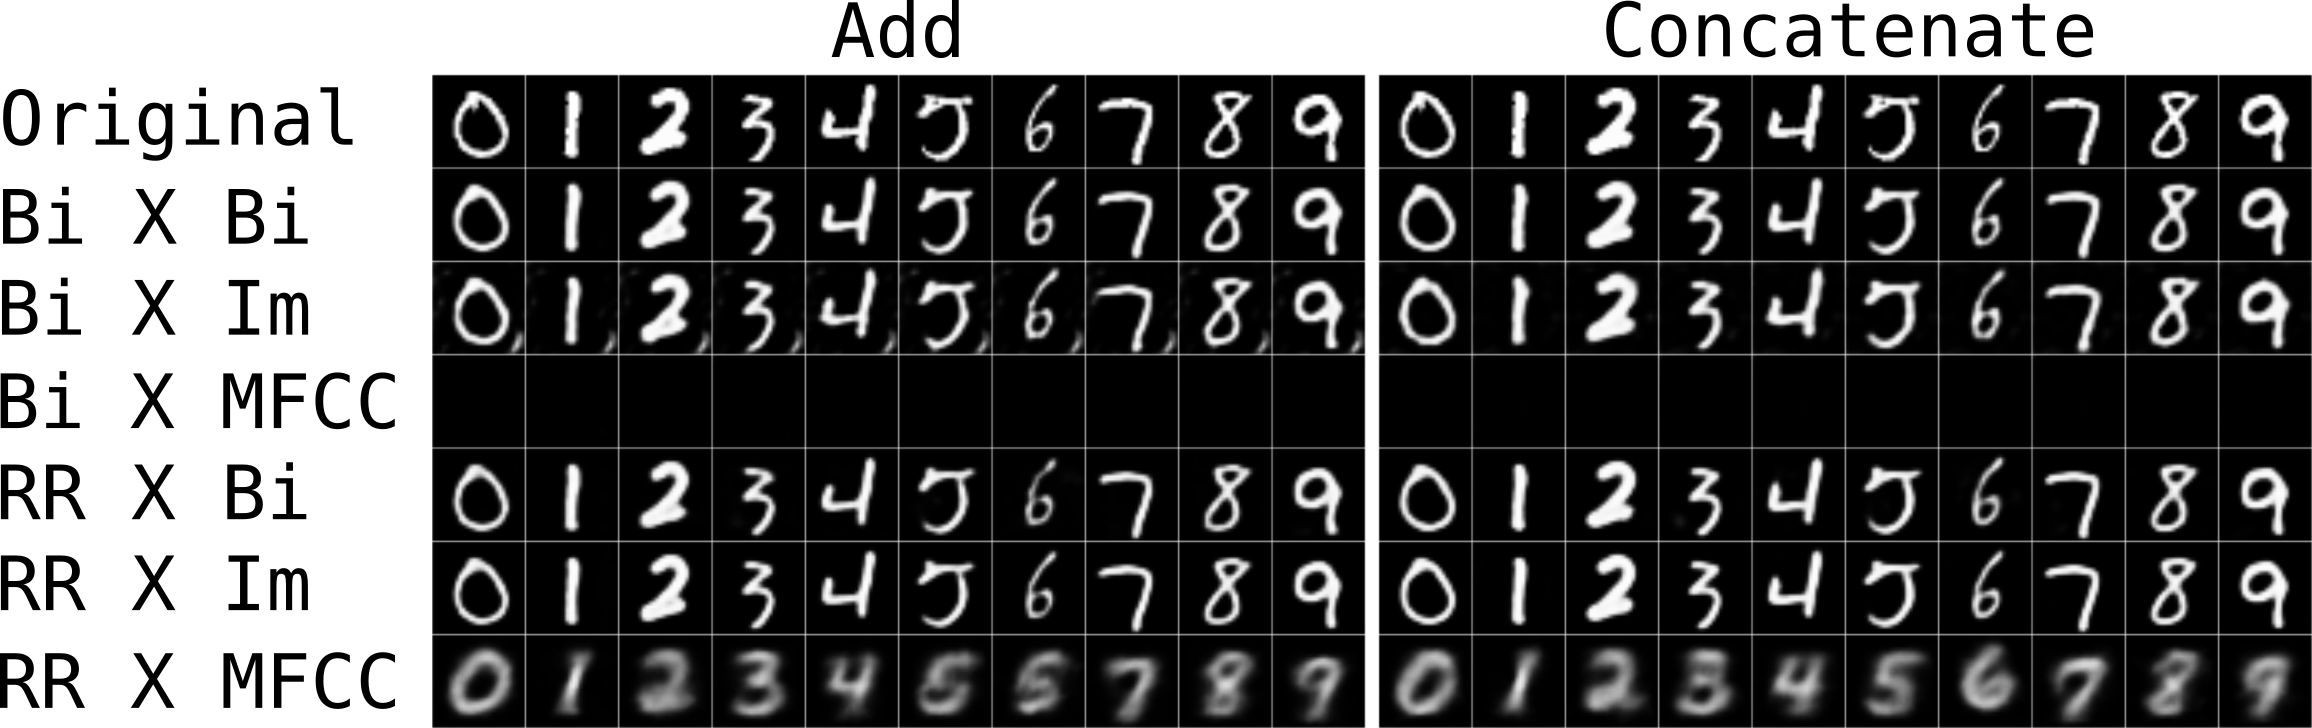
\includegraphics[width=\textwidth]{Figs/mnistSpoken/lbAll.png}
	\caption{A selection of randomly sampled digits generated in different training and testing conditions for both \textit{Add} and \textit{Concat} merging methods.}
	\label{fig:mnistDigits}
\end{center}
\end{figure}

\autoref{fig:5s} shows a comparison of two different examples of the digit ``5''. One is (subjectively) poorly written and the other is more prototypical and well formed. Under different testing conditions, the \acp{MAE} regenerate different ``fives''.

\begin{figure}[h]
\begin{center}
	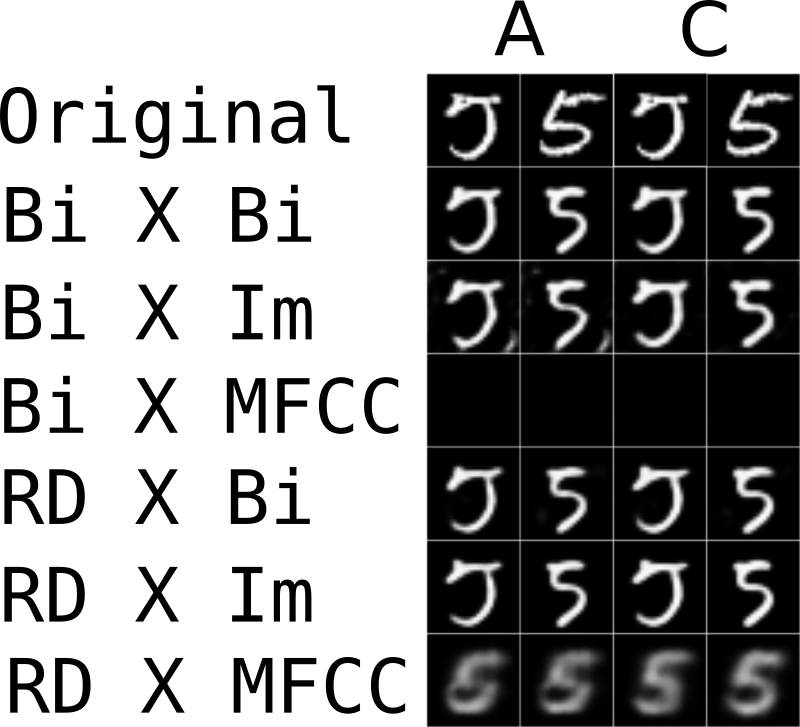
\includegraphics{Figs/mnistSpoken/5s.png}
	\caption{Two examples of the digit ``5'' being generated in different training and testing conditions for both \textit{Add} and \textit{Concat} merging methods.}
	\label{fig:5s}
\end{center}
\end{figure}



\subsection{Discussion}

\subsubsection{Discussion of Classification Results}
\autoref{tab:mnist_ucu_bi_res} shows that both the \textit{Add} and \textit{Concat} \acp{MAE} have better classification accuracy than the baseline, unimodal models. However, it is not clear that there is a difference between the two training procedures, Bi and RR.

The difference between the two training procedures becomes clear in \autoref{tab:mnist_ucu_im_res} where it can be seen that the \acp{MAE} trained using the Bi training procedure have lower classification rates when presented with only images as input. Models perform less than half as well as the baseline model, 0.4501 (\textit{Add}) and 0.3496 (\textbf{Concat}) versus 0.9832 for the baseline image autoencoder.

There is a trade off between unimodal accuracy and mulitmodal accuracy in the RR training procedure \acp{MAE}. Whilst both the \textit{Add} and \textit{Concat} \acp{MAE} outperform the baseline models in the Bimodal test condition, they have slightly worse performance when tested with either images or \acp{MFCC} only. For example, the best performance is given by the \textit{Add} \ac{MAE} under the RR training procedure when both images and \acp{MFCC} are present as inputs, with an accuracy of 0.9993. However, if one of the modalities is removed, the accuracy drops to 0.9834 and 0.9789 for Image Only and \ac{MFCC} Only testing respectively. Comparing this to the baseline unimodal models, which have classification accuracies of 0.9883 and 0.9832 for image and \ac{MFCC} autoencoders respectively, it can be seen that there is a small decrease in performance for the MAEs tested with unimodal data compared to the unimodal baselines. 

There is a drop of 0.0049 and 0.0043 for Image Only and \ac{MFCC} Only testing using the \textit{Add} \ac{MAE}. However, this reduction in performance is conterbalanced by the improvement in performnace when both modalities are present, 0.9993 versus the 0.9883 and 0.9832 of the baseline models. This improvement of 0.0110 to 0.0161 over the baseline image and \ac{MFCC} autoencoders is more than twice the decrease in performance when only one modality is available. 

Specifically, the improvement of Bimodal classification is 2.24 times larger than the decrease in performance when only images are available ($0.011 / 0.0049 = 2.24$). Comparing to the \ac{MFCC} baseline, the Bimodal performance improvement is 3.74 times larger than the decrease in performance when only \acp{MFCC} are available.

\subsubsection{Discussion of Reconstruction Results}
Observing \autoref{tab:mnist_ucu_bi_res}, \autoref{tab:mnist_ucu_im_res} and \autoref{tab:mnist_ucu_mfcc_res} it can be seen that different models have different reconstruction errors (Mean Squared Error). Whilst all \ac{MAE} models had higher reconstruction errors than the baseline models, this is to be expected. The \ac{MAE} models are trading off between representing each modality well, whilst the unimodal autoencoders that give the baseline numbers can use their full capacity to minimise the reconstruction error of their one modaility, as they do not have to reconstruct the second modality. 

That being said, the image reconstruction error is comparable across all \ac{MAE} models, approximately 0.0031, (see table \autoref{tab:mnist_ucu_bi_res} and is very close to the baseline of 0.0027 under the Bimodal testing condition (i.e. when the images to be reconstructed are available as input). Further to this, the image reconstruction error for the \ac{MFCC} Only testing condition is still small (0.0554), though an order of magnitude worse, for the \acp{MAE} trained using the RR procedure.

\paragraph{Image reconstruction from MFCCs}
The increase in image reconstruction error when only \acp{MFCC} are provided as input is due to the construction of an internal symbolic language which represents the meaning of both the utterances (\acp{MFCC}) and images but not necessarily their fine details. For example, looking at \autoref{fig:5s} we see that there are different ways to write the number 5, however both of these images have the same meaning, ``five''. It is more important to preserve this meaning than the minutia of the original images. The same can also be said for reconstructing \acp{MFCC}, their meaning is more important than their exact enunciation.  

The \ac{MFCC} reconstruction error is best for the baseline model but is only 4.0265 times worse for the best performing model on this task. Considering how small the baseline error is, being four times worse, is still good performance, especially considering the difficulty of the task.

\paragraph{MFCC reconstruction from Images}
The \ac{MFCC} reconstruction error is an order of magnitude worse than the image reconstruction error. In part this is due to the nature of the data, as seen by the difference in baseline reconstruction errors. It appears to be more difficult to reconstruct \acp{MFCC} than images, even when \acp{MFCC} are given as input.

Another contributing factor to the worse \ac{MFCC} reconstruction error for the \acp{MAE}, is the inbalance between sample numbers for MNIST and UCU. Whilst both datasets are balanced within themselves (there are an equal number of training samples for each class) there is a big difference between the sizes of MNIST and UCU. 

The difference in sizes between the datasets means that reconstructing \acp{MFCC} from image inputs will map a large number of inputs to a smaller number of outputs and vice-versa for generating images from \ac{MFCC} inputs. Therefore images in the test set which look similar to images in the training set, will be mapped to \acp{MFCC} similar to those which the training images map too. As there are a smaller number of \ac{MFCC} examples to map to, our output is less likely to be normally distributed. Whilst idealy we would like to map similar looking digits to similar sounding utterances, there is no gaurantee that this is true, either in our dataset or in general. People with similar handwritting don't necessarily have similar voices. This is simulated by the random assignment of images to \acp{MFCC} but this results in discontinuities in the latent space of the network, particularly with respect to generating \acp{MFCC}, of which we have fewer examples to capture the true distribution of the data.

Conversely, as there are more examples of images of digits, the distribution of the latent space with respect to the images can get closer to modelling the real distribution of the images. Therefore, given a test \ac{MFCC}, regardless of whether it is similar to a training \ac{MFCC} example, its target image, is more likely to be similar to images in the training data. 

\paragraph{Effects of randomly removing inputs}
\autoref{fig:mnistDigits} shows that randomly removing the training data has a significant effect, beyond just the improvements to classification accuracy seen in \autoref{tab:mnist_ucu_bi_res}, \autoref{tab:mnist_ucu_im_res} and \autoref{tab:mnist_ucu_mfcc_res}. Both the \textit{Add} and \textit{Concat} \acp{MAE} fail to learn to generate images from \ac{MFCC} data using the Bi training procedure.

Comparing the images generated by the \textit{Add} and \textit{Concat} \acp{MAE} (\autoref{fig:mnistDigits}) for the \ac{MFCC} test condition when the training data has been Randomly Removed, it can be seen that the \textit{Concat} \ac{MAE} outperforms the \textit{Add} MAE. This is particularly clear when you look at the ``five'' and ``six'' generated by the \textit{Add} \ac{MAE} for RR X \ac{MFCC}, where the \ac{MAE} has failed to correctly generate a ``six'' and has instead generated a ``five'', which is similar to the prototypical five generated when \acp{MFCC} for a five are presented.
Unlike the \textit{Add} \ac{MAE}, the \textit{Concat} \ac{MAE}, correctly generates all digits, including ``six''.

\paragraph{Multiple generations of the same digit}
In \autoref{fig:5s} we see that different examples of the same digit produce different generation results. Most interestingly however, are the generated ``fives'' shown in the RR X MFCC row. A more prototypical ``five'' is generated from \acp{MFCC} than if an image of a non-prototypical five is given. This shows that the meaning of the \acp{MFCC} have been grounded in the image modality and that an internal symbolic language has been learnt, i.e. the latent embedding of \acp{MFCC} are a symbolic representation which has meaning in both \ac{MFCC} and image space, hence the ability to generate meaningful images and \acp{MFCC} from these embeddings.

\section{Summary}
In this chapter I set out to demonstrate the advantages of multimodality as applied to classification and regeneration of missing data.

Whilst multimodal systems can provide better classification accuracy, this comes at the cost of a higher computational burden and, lower classification accuracy when only one modality is available, as demonstrated by the results presented in this chapter.

The ability to reconstruct missing data from a secondary modality demonstrates how an internal symbolic language can be learnt in an unsupervised fashion by processing aligned percepts in multiple modalities.

In future it would be worth while to observe how the reconstructed data can be exploited to improve classification accuracy, for example by first generating a missing data points from modality A and then performing a classification on the embedding of data from modality B and the generated modality A.

This experiment lays the ground work for the next chapter where I will look at how a more complex internal symbolic language can be developed and exploited.

Further discussion of the results from this chapter have been published in \cite{sheppardtowards}. 
%I will also discuss how this can be applied to creating robots capable of life long learning. 
\theendnotes
%% Chapter Template

\chapter{Magical Vectors and Where to Find Them} % Main chapter title

\label{Chapter5} % Change X to a consecutive number; for referencing this chapter elsewhere, use \ref{ChapterX}

\lhead{Chapter 5. \emph{Magical Vectors and Where to Find Them}} % Change X to a consecutive number; this is for the header on each page - perhaps a shortened title

\section{ANN Latent space: the Final Frontier}
One of the most interesting properties of neural networks is the latent embeddings they learn which are abstract representations of the input data. The embedding of a given data sample, is the activation of the neural network at a specific layer within the network. In the case of MAEs this is the layer after which the different modalities have been merged.

Normally when working with neural networks we are very interested in the output of the neural network, for example, does the network correctly classify an image and how confident it is - this is the whole reason for using cross-entropy losses for training. However, in my case, I am more interested in how the neural network represents what it has learnt.

In \cite{mikolov2013distributed} and \cite{mikolov2013efficient}, it is demonstrated that skipgram models trained on large corpuses develop word embeddings whose embeddings in the latent embedding space tell us something about the relational meanings of the words the embeddings belong to. For example questions such as \textit{``King is to man as woman is to...''} can be solved with some vector arithmetic on these embeddings as shown in \autoref{eqn:mikolov}.
\begin{equation}
emb(king) - emb(man) + emb(woman) \approx emb(Queen)
\label{eqn:mikolov}
\end{equation} 

The embeddings learnt by skipgram models show clusterings of different word types, such as nouns, verbs and adverbs whilst things like capital cities and country names form their own subclusters within the larger cluster of all nouns. Whilst the model does not know the meaning of any of the words it has learnt to embed, clearly it has divided the embedding space in a useful way and if symbol grounding can be performed on some of the words, this will provide a basis to start producing models which do know the meaning of the words they are embedding.

To that end, I will now demonstrate how a MAE can be used to learn multimodal representations of words and the visual attributes they equate to in order to solve the symbol grounding problem in an unsupervised manner.

Further to this, I will show how taking an incremental approach to learning improves the quality of the bidirectional symbol grounding. Visual attibutes are more accurately described and better images are generated from descriptions by MAEs which have first been pretrained on a subset of visual attributes and descriptions compared to the randomly initialised baseline models.

\section{Vector Arithmetic}
The embeddings learnt by the MAE can be manipulated to generate novel images. For example, once the MAE is trained, we can easily add and subtract the embeddings of images and words from one and other. \autoref{fig:vectorArthexmp} demonstrates how the embedding of an image can be changed using the embeddings of words in order to alter the colour of the image. It should be noted that this method can be applied to any attribute of the image, not just colour but also, shape, size and position, and is independant of the input modality (we can add and subtract embeddings of images or words).

\begin{figure}
\centering
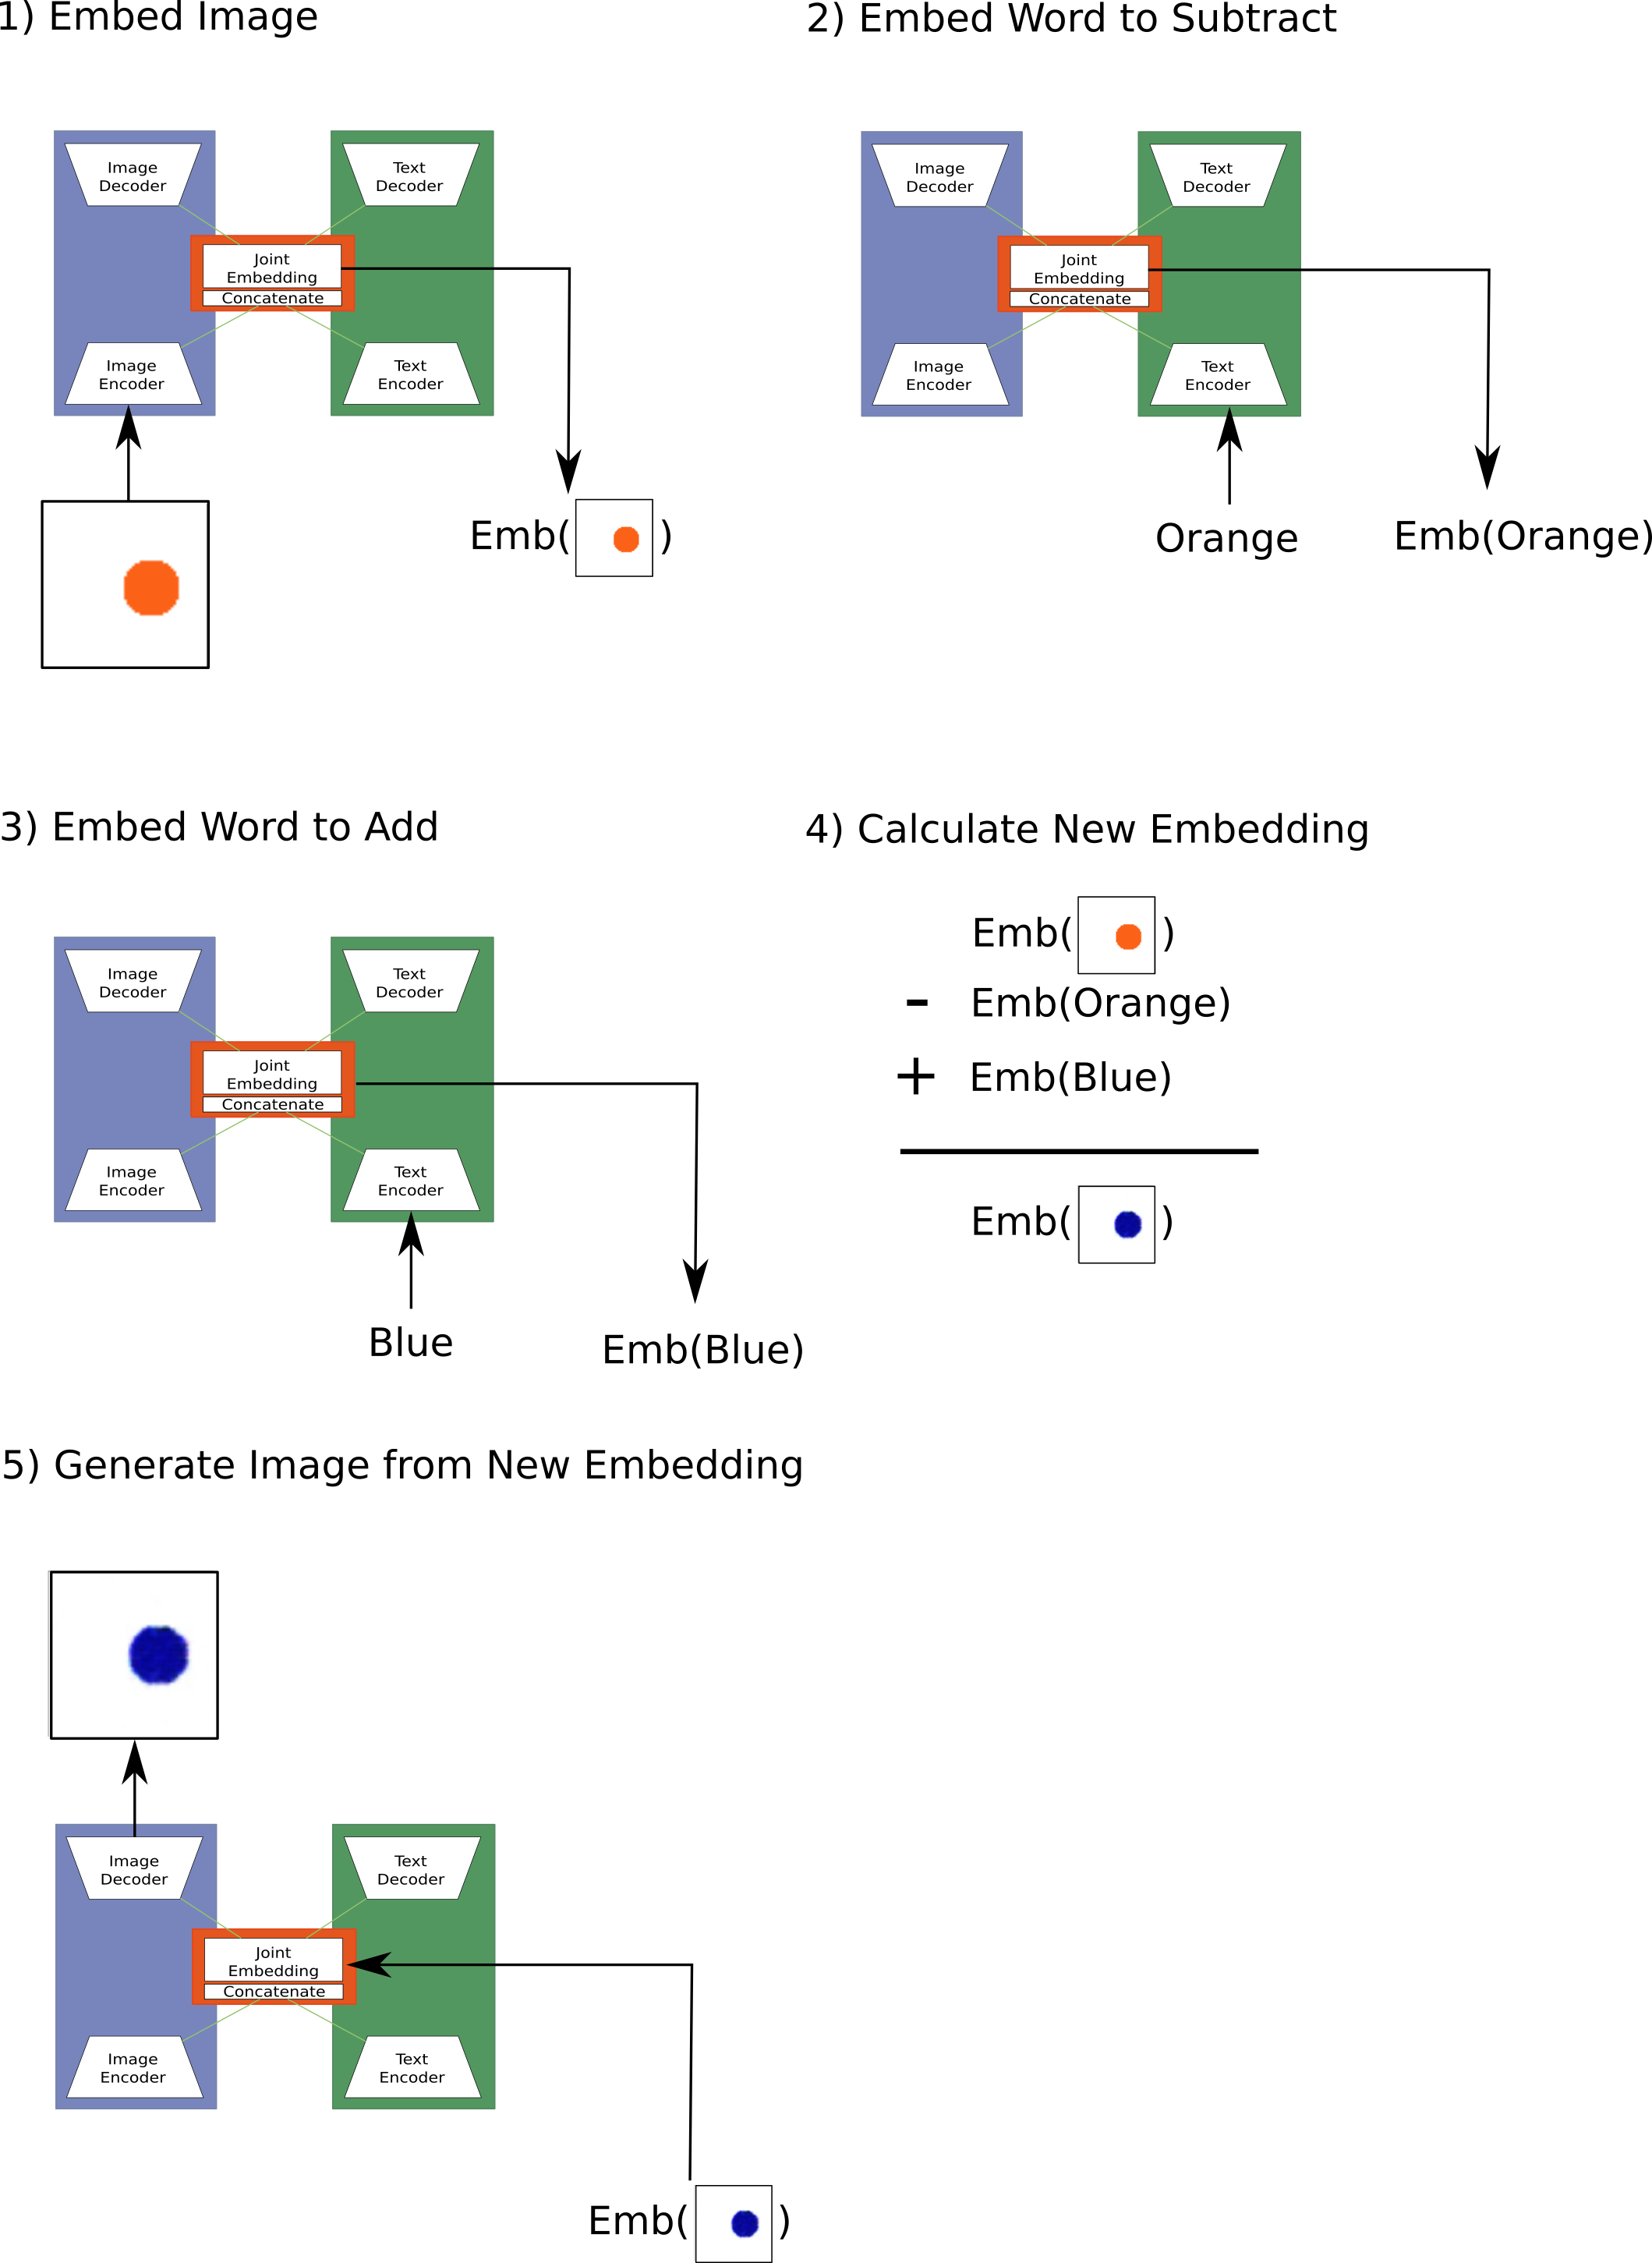
\includegraphics[width=\textwidth]{Figs/shapes/vectorArthExmp.png}
\caption{An example of how novel images can be generated using Vector Arithmetic on image and word embeddings.}
\label{fig:vectorArthexmp}
\end{figure}

\begin{figure}
\centering
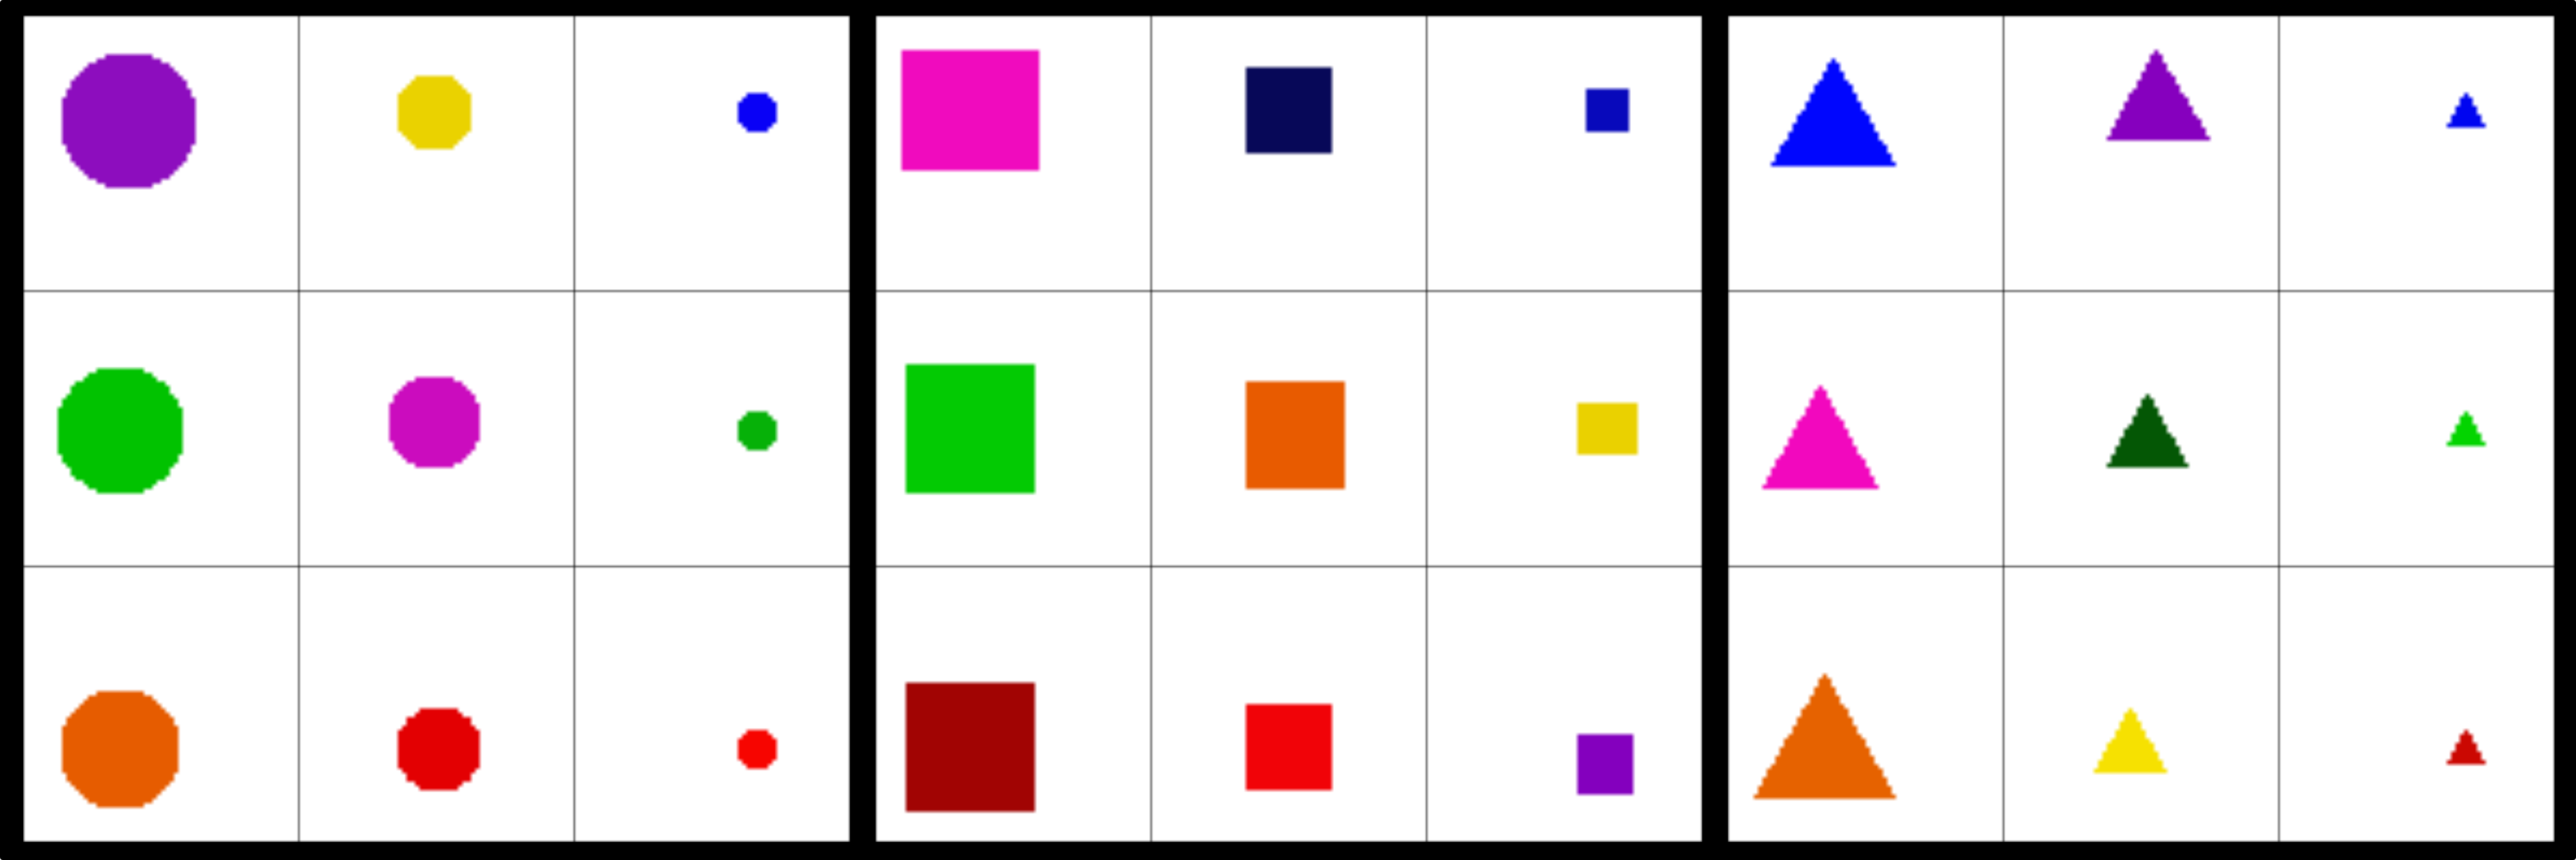
\includegraphics[width=0.75\textwidth]{Figs/shapes/shapes.png}
\caption{Examples of the different, shapes, colours, sizes and positions of objects in the ArtS dataset. The top left object would be described as ``big indigo circle, top left''.}
\label{fig:shapes}
\end{figure}

\newpage
\section{Artificial Shapes Dataset}
\subsection{Dataset Description}
The Artificial Shapes dataset (ArtS) contains images and simple descriptions of the images. The dataset is artificially generated using a Python script, each image is 64x64 pixels and is described by the shape, colour, size and position of the object in the image. Additionally, the RGB value of the colour and the coordinates of the centre of the object are available, though these are not used in the following experiments. 

\begin{table}[h]
\centering
\begin{tabular}{|c|c|}
\hline
\textbf{Attribute} & \textbf{Description} \\ \hline \hline
\textbf{Shapes} & \textbf{Corners} \\ \hline
Circle (Circ) & 0\\ \hline 
Rectangle (Rect) & 4\\ \hline
Triangle (Tri)& 3\\ \hline

\textbf{Colours} & \textbf{RGB Values}	\\ \hline	
Red (r)& (75,0,0) - (255, 10, 10)\\ \hline
Orange (o) & (225,75,0) - (255, 155, 50)\\ \hline
Yellow (y) & (230,200,0) - (255, 255, 95)\\ \hline
Green  (g)& (0,75,0) - (10, 255, 10)\\ \hline
Blue   (b)& (0,0,75) - (10, 10, 255)\\ \hline
Indigo (i)& (90,0,190) - (150, 50, 255)\\ \hline
Violet (v)& (200,0,190) - (255, 50, 255)\\ \hline 

\textbf{Sizes} & 	\textbf{Length/Radius (pixels)} \\ \hline			  
Big    (B)& 32 - 35  \\ \hline
Medium (M)& 22 - 25 \\ \hline
Small  (S)& 12 - 15 \\ \hline 

\textbf{Positions} & \textbf{Object Centre Coordinate}	\\ \hline					  
Top Left (TL)& (22,42)\\ \hline	
Top Centre (TC)& (32,42)\\ \hline
Top Right (TR)& (42,42)\\ \hline
Centre Left (CL)&(22,32)\\ \hline
Centre Centre (CC) & (32,32)\\ \hline
Centre Right (CR)&(42,32)\\ \hline
Bottom Left (BL)& (22,22)\\ \hline
Bottom Centre (BC)& (22,42)\\ \hline
Bottom Right (BR)& (42,22)\\ \hline				
\end{tabular}
\caption{Artificial Shapes dataset description.}
\label{tab:Arts_desc} 
\end{table}

To help differentiate between words, visual attributes and the abstract concepts they represent the following notation will be used: the words of the descriptions will be written using \textsc{small capitals}, visual attributes (shapes, colours, sizes and positions) are written using \textit{capitalised italics} any other times words which could appear in the description of an image from ArtS that are not formatted as either \textsc{small capitals} or \textit{capitalised italics} are normal uses of these words and do not refer to either descriptions or visual attributes.
For example the word ``blue'' from a description will appear as \textsc{blue} and the colour ``blue'' will appear as \textit{Blue}. 


The dataset contains 3 different shapes, \textit{Rectangle}, \textit{Triangle} and \textit{Circle}. Each of these shapes comes in 7 colours, 3 sizes and 9 positions as described in \autoref{tab:Arts_desc}. Each colour covers a range of values, the RGB value for each object in the ArtS dataset is randomly selected from the ranges described in the ``Description'' column of \autoref{tab:Arts_desc}. Whilst the centre of each object is fixed based on its position, the exact size is not fixed based on its size category. The size categories \textit{Big}, \textit{Medium} and \textit{Small} do not describe fixed radiuses and lengths, there is some variation in the values of these for each category.


\autoref{fig:shapes} shows some example images from the ArtS dataset for each of the 3 shapes, 7 colours, 3 sizes and 9 positions.

\subsection{Problem Description}
Using the ArtS dataset, I will demonstrate that it is possible to learn a joint, multimodal representation of the images and their descriptions. Once this representation is learnt, I will demonstrate that we can correctly label novel images with their descriptions and also that we can generate correct images from descriptions.

In the previous chapter, we saw a similar problem which was broken into two subproblems, classification and bidirectional symbol grounding. With this dataset we are not interested in performing a classification as the classification is encapsulated in the generation of correct descriptions for novel images. I will therefore be demonstrating how bidirectional symbol grounding circumvents the need for classification by providing a high level understanding of the meaning of an instance of a modality rather than just a predefined class for that instance. E.g. the neural network is not simply assigning images of \textit{Rectangles} to the Rectangles class, but instead learn what the meanings of the word \textsc{Rectangle} and the visual property \textit{Rectangle} are. 

Further to this, I will demonstrate that once trained, the neural network can infer the meaning of unseen descriptions to correctly generate images and vice-versa. If we omit a subcategory of object from the training data, for example violet circles, the neural network is still able to generate images of violet circles as it has grounded the meaning of both \textsc{Blue} and \textsc{Circle} as well as the visual properties \textit{Blue} and \textit{Circle}. It is also able to correctly label images of blue circles for the same reason, despite never having never seen what a blue circle is.


\subsection{Network Description}
The overall structure of the neural netwrok used for the experiements in this chapter is very similar to the one used in \autoref{Chapter4}, with two inputs for each of the different modalities, this time, images and words. However, it only has two outputs, one for images and one for words, unlike in the previous chapter where we also had a third output which acted as a classification layer. \autoref{tab:Arts_MAE_description} in \autoref{appendix:B} gives the specific details on each of the layers of the network. Additionally, batchnormalisation is used between beach convolution layer.



\section{Experiments with the ArtS Dataset}
For each of the following experiments I will test the MAE in three ways, similarly to the experimental method of \autoref{Chapter4}. Following the protocol of testing in a Bimodal, Image Only and Words Only manner allows me to explore how each of the modalities and their combination, affects the quality of the embedding learnt by the neural network. All experiments in this section will utilise the RD training procedure developed in \autoref{chapter4}.


Due to the complexity of ArtS and the variety of factors which can be explored with it, I will perform 5 sets of experiments, each using different subsets of the dataset. All experiments will make use of all 3 shapes, but different numbers of colours, sizes and positions will be used.

Each experiment is four fold cross validated using randomly selected training data and weight initialisations.

\subsection{Experiment 1}
The first experiment will utilise 3 colours, 3 positions and 1 size as shown in \autoref{tab:exp1_data}. The aim of this experiment is to find the best size for the embedding layer. I wish to find a number of filters which minimises the reconstruction loss for both the images and descriptions under all testing conditions. Futher to this I also wish to find an embedding size which allows for the accurate grounding of all words in the dataset. For example, if the MAE is given only the word \textsc{Blue} I want it to generate a \textit{Blue} image, or given the word \textsc{Triangle} an image of a \textit{Triangle}. 

Each shape-colour-size-position combination will be referred to as an object.

For each object, I will generate 50 training samples giving a total of 1350 training samples. The validation and testing data consist of 100 samples per object giving 2700 validation and 2700 testing samples.



\begin{table}[ht]
\centering
\begin{tabular}{|c|c|}
\hline
\textbf{Attribute} & \textbf{Description} \\ \hline \hline
\textbf{Shapes} & \textbf{Corners} \\ \hline
Rectangle & 4\\ \hline
Triangle & 3\\ \hline
Circle & 0\\ \hline 

\textbf{Colours} & \textbf{RGB Values}	\\ \hline	
Red & (75,0,0) - (255, 10, 10)\\ \hline
Green  & (0,75,0) - (10, 255, 10)\\ \hline
Blue   & (0,0,75) - (10, 10, 255)\\ \hline


\textbf{Size} & 	\textbf{Length/Radius (pixels)} \\ \hline			  
Big    & 32 - 35  \\ \hline


\textbf{Positions} & \textbf{Object Centre Coordinate}	\\ \hline				  
Centre Left &(22,32)\\ \hline
Centre Centre & (32,32)\\ \hline
Centre Right &(42,32)\\ \hline
				
\end{tabular}
\caption{Experiment 1 data subset.}
\label{tab:exp1_data} 
\end{table}

\subsubsection{Results}

The affect of increasing the embedding size is mostly to improve the reconstruction error for images, in the Bimodal and Image Only testing conditions as shown by the blue and brown lines in \autoref{fig:graph331} (B). The reconstruction of images from their descriptions is only affected a very small amount by the size of the embedding. With the exception of when the embedding is very small, the description to image reconstruction errors only vary a small amount with respect to the embedding size (red line in \autoref{fig:graph331}). 

\begin{figure}[h]
\centering
\resizebox{0.75\textwidth}{!}{
\begin{tikzpicture}
    \begin{axis}[
     name=plot1,
     axis x line=middle,
     axis y line=middle,
     enlarge y limits=true,
     enlarge x limits=true,
     legend style={at={(0.5,-0.5)}, anchor=north},
     %xmin=0, xmax=2150,
     %ymin=0, ymax=600,
     %width=15cm, height=8cm,     % size of the image
     grid = major,
     grid style={dashed, gray!30},
     ylabel= Total MSE,
     %ytick={0,0.001,0.002,0.003,0.004,0.005,0.006,0.007,0.008,0.009},
     xlabel= (A) Embedding Size,
     %xtick={6,8,10,12,14,16,18,20,22,24,26,28,30,32,34,35,36,37,38,39,40,41,42,43,44,45,46,47,48,49,50,51,52,53,54,55,56},     
	 xlabel near ticks,
	 ylabel near ticks]
         ] 
    ]
    \addplot table[x = size, y = bimodal, col sep = comma]{csvs/331/total331.csv}; 
    \addplot table[x = size, y = words only, col sep = comma]{csvs/331/total331.csv};
    \addplot table[x = size, y = image only, col sep = comma]{csvs/331/total331.csv};    
    \legend{Bimodal, Words Only, Image Only}
    
    \end{axis}
    
    
     \begin{axis}[
     name=plot2,
     at=(plot1.right of south east), 
     anchor=left of south west,
     axis x line=middle,
     axis y line=middle,
     enlarge y limits=true,
     enlarge x limits=true,
     %legend style={at={(1,0.7)}, anchor=north},
     %xmin=0, xmax=2150,
     %ymin=0, ymax=600,
     %width=15cm, height=8cm,     % size of the image
     grid = major,
     grid style={dashed, gray!30},
     ylabel= Image MSE,
     %ytick={0,0.001,0.002,0.003,0.004,0.005,0.006,0.007,0.008,0.009},
     xlabel= (B) Embedding Size,
     %xtick={6,8,10,12,14,16,18,20,22,24,26,28,30,32,34,35,36,37,38,39,40,41,42,43,44,45,46,47,48,49,50,51,52,53,54,55,56},     
     xlabel near ticks,
	 ylabel near ticks]
         ] 
    ]
    \addplot table[x = size, y = bimodal, col sep = comma]{csvs/331/image331.csv}; 
    \addplot table[x = size, y = words only, col sep = comma]{csvs/331/image331.csv};
    \addplot table[x = size, y = image only, col sep = comma]{csvs/331/image331.csv}; 
       
    %\legend{Bimodal, Words Only, Image Only}
    \end{axis}
    
	
    
    \begin{axis}[
     name=plot3,
     at=(plot2.below south west),
     anchor=above north west,
     axis x line=middle,
     axis y line=middle,
     enlarge y limits=true,
     enlarge x limits=true,
     %legend style={at={(1,0.7)}, anchor=north},
     %xmin=0, xmax=2150,
     %ymin=0, ymax=600,
     %width=15cm, height=8cm,     % size of the image
     grid = major,
     grid style={dashed, gray!30},
     ylabel= Word MSE,
     %ytick={0,0.001,0.002,0.003,0.004,0.005,0.006,0.007,0.008,0.009},
     xlabel= (C) Embedding Size,
     %xtick={6,8,10,12,14,16,18,20,22,24,26,28,30,32,34,35,36,37,38,39,40,41,42,43,44,45,46,47,48,49,50,51,52,53,54,55,56},     
     xlabel near ticks,
	 ylabel near ticks]
         ] 
    ]
    \addplot table[x = size, y = bimodal, col sep = comma]{csvs/331/word331.csv}; 
    \addplot table[x = size, y = words only, col sep = comma]{csvs/331/word331.csv};
    \addplot table[x = size, y = image only, col sep = comma]{csvs/331/word331.csv};    
    %\legend{Bimodal, Words Only, Image Only}
    \end{axis}
    

\end{tikzpicture}
}
\caption{Experiment 1: MSE for reconstruction of images and descriptions under different testing conditions. (A) shows the total MSE, (B) shows the MSE of the image output and (C) shows the MSE of the word output.}
\label{fig:graph331}
\end{figure}


\begin{table}[h]
\centering
	\begin{tabular}{|c|c|c|c|}
	\hline
	Size & 	Bimodal	 & 	Image Only	& 	Words Only \\ \hline
8	&	9.17	$\mypm$	0.58	&	9.26	$\mypm$	0.76	&	9.70	$\mypm$	0.67	\\ \hline
40	&	8.33	$\mypm$	0.14	&	7.91	$\mypm$	0.14	&	8.59	$\mypm$	0.13	\\ \hline
72	&	8.09	$\mypm$	0.16	&	7.64	$\mypm$	0.16	&	8.40	$\mypm$	0.14	\\ \hline
104	&	7.69	$\mypm$	0.43	&	7.04	$\mypm$	0.49	&	8.40	$\mypm$	0.24	\\ \hline
136	&	7.14	$\mypm$	0.58	&	6.45	$\mypm$	0.74	&	8.41	$\mypm$	0.16	\\ \hline
168	&	7.01	$\mypm$	0.61	&	6.28	$\mypm$	0.65	&	8.38	$\mypm$	0.17	\\ \hline
200	&	\textbf{6.80}	$\mypm$	0.27	&	\textbf{6.10}	$\mypm$	0.33	&	\textbf{8.30}	$\mypm$	0.17	\\ \hline
232	&	6.97	$\mypm$	0.64	&	6.28	$\mypm$	0.68	&	8.55	$\mypm$	0.05	\\ \hline
264	&	6.92	$\mypm$	0.92	&	6.32	$\mypm$	0.97	&	8.45	$\mypm$	0.24	\\ \hline
296	&	\textbf{6.80}	$\mypm$	1.11	&	6.15	$\mypm$	1.18	&	8.64	$\mypm$	0.27	\\ \hline

	\end{tabular}
\caption{Experiment 1: Total MSE for different embedding sizes for the three testing conditions. An Embedding Size of 200 neurons provides the minimum reconstruction error. (All values are $\times10^{-3}$)}
\label{tab:res331}
\end{table}

\autoref{tab:res331} allows a closer look at the values of the total error (the sum of image and description reconstruction errors) for the different testing conditions. An embedding size of 200 neurons provides the best total loss in all testing conditions. This performance is matched by an embedding size of 296 neurons in the Bimodal testing condition, however it has a much larger standard deviation as it performs significantly better than the smaller embedding size in the best run but also much worse in the worst run.


From the numerical results presented in \autoref{tab:res331} it is clear that the majority of the error comes from the image output. This is expected as the dimensionality of the images is much larger than the description output (64x64x3 vs 22x1). Notice in particular the scale of the errors in \autoref{fig:graph331}, the image output loss is of a scale $10^{-2}$ compared to the description output which has a scale of $10^{-5}$, three orders of magnitude smaller. 

There is a limit to how good the images reconstructed from descriptions can be as the descriptions do not contain all of the information necessary to perfectly reconstruct the images. This shows up as the difference between image reconstruction in the Image Only testing condition vs the Words Only condition. Put simply, this difference is caused by the standard deviation within the colours and sizes of the objects. 

Whilst the images generated in the Image Only and Bimodal testing conditions have access to exact RGB values and sizes, the descriptions only contain the name of the colour of the object and can therefore only produce objects with the ``average'' RGB values for those words, learnt from the training data. For example, looking at \autoref{tab:exp1_data} we see that the colour \textit{Red} can have RGB values anywhere in the range (75,0,0) - (255, 10, 10).

The standard deviation across the fours runs of the experiment is very low for all embedding sizes, showing that the images generated by the MAE are independent of the starting weights and the randomly selected training data from the ArtS dataset. 

\paragraph{Image Generation}

Generating images from full descriptions gives very good quality results as seen in \autoref{fig:331multi}. Here we see images generated with an embedding size of 200 neurons. From \autoref{tab:res331} we can see that 200 gave the best reconstruction error in the Bimodal, Image Only and Words Only testing conditions. However, the small changes in reconstruction error in the Words Only testing condition are negligble when considering that the semantic information contained in the images is always correct regardless of embedding size. Each description leads to the generation of an image which clearly matches its descriptions, regardless of the embedding size. 

\begin{figure}
\centering
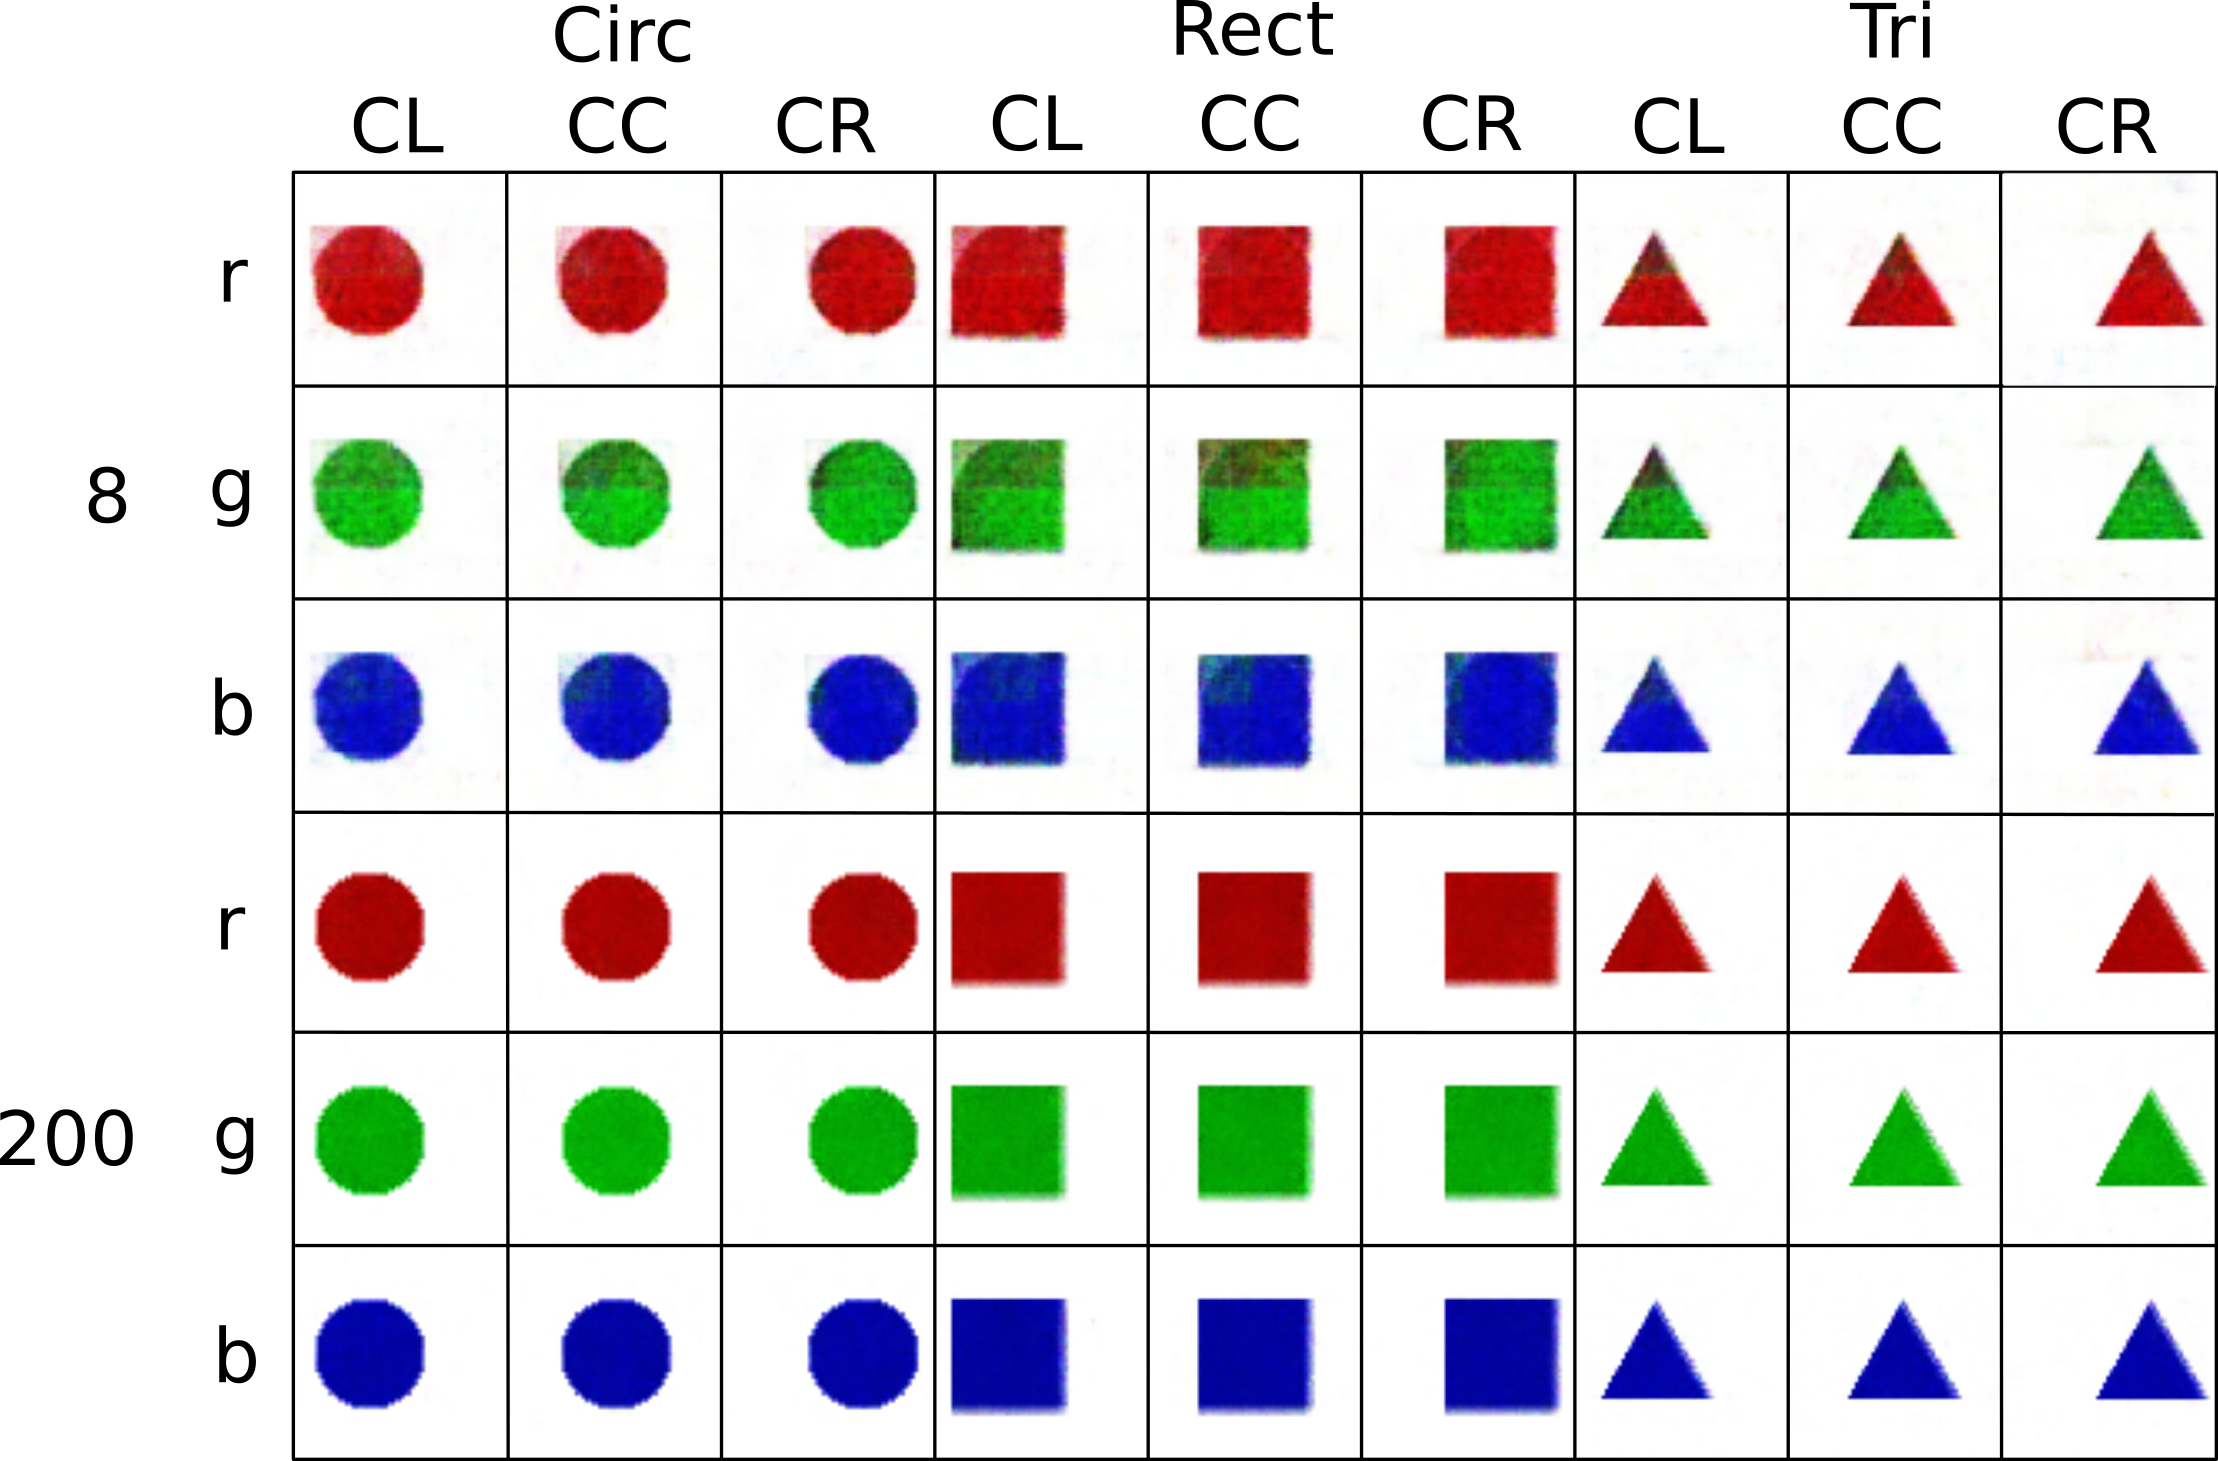
\includegraphics[width=0.625\textwidth]{Figs/shapes/331_8v200.png}
\caption{Images generated from descriptions with an embedding size of 8 or 200.}
\label{fig:331multi}
\end{figure}

%\begin{figure}[h]
%\centering
%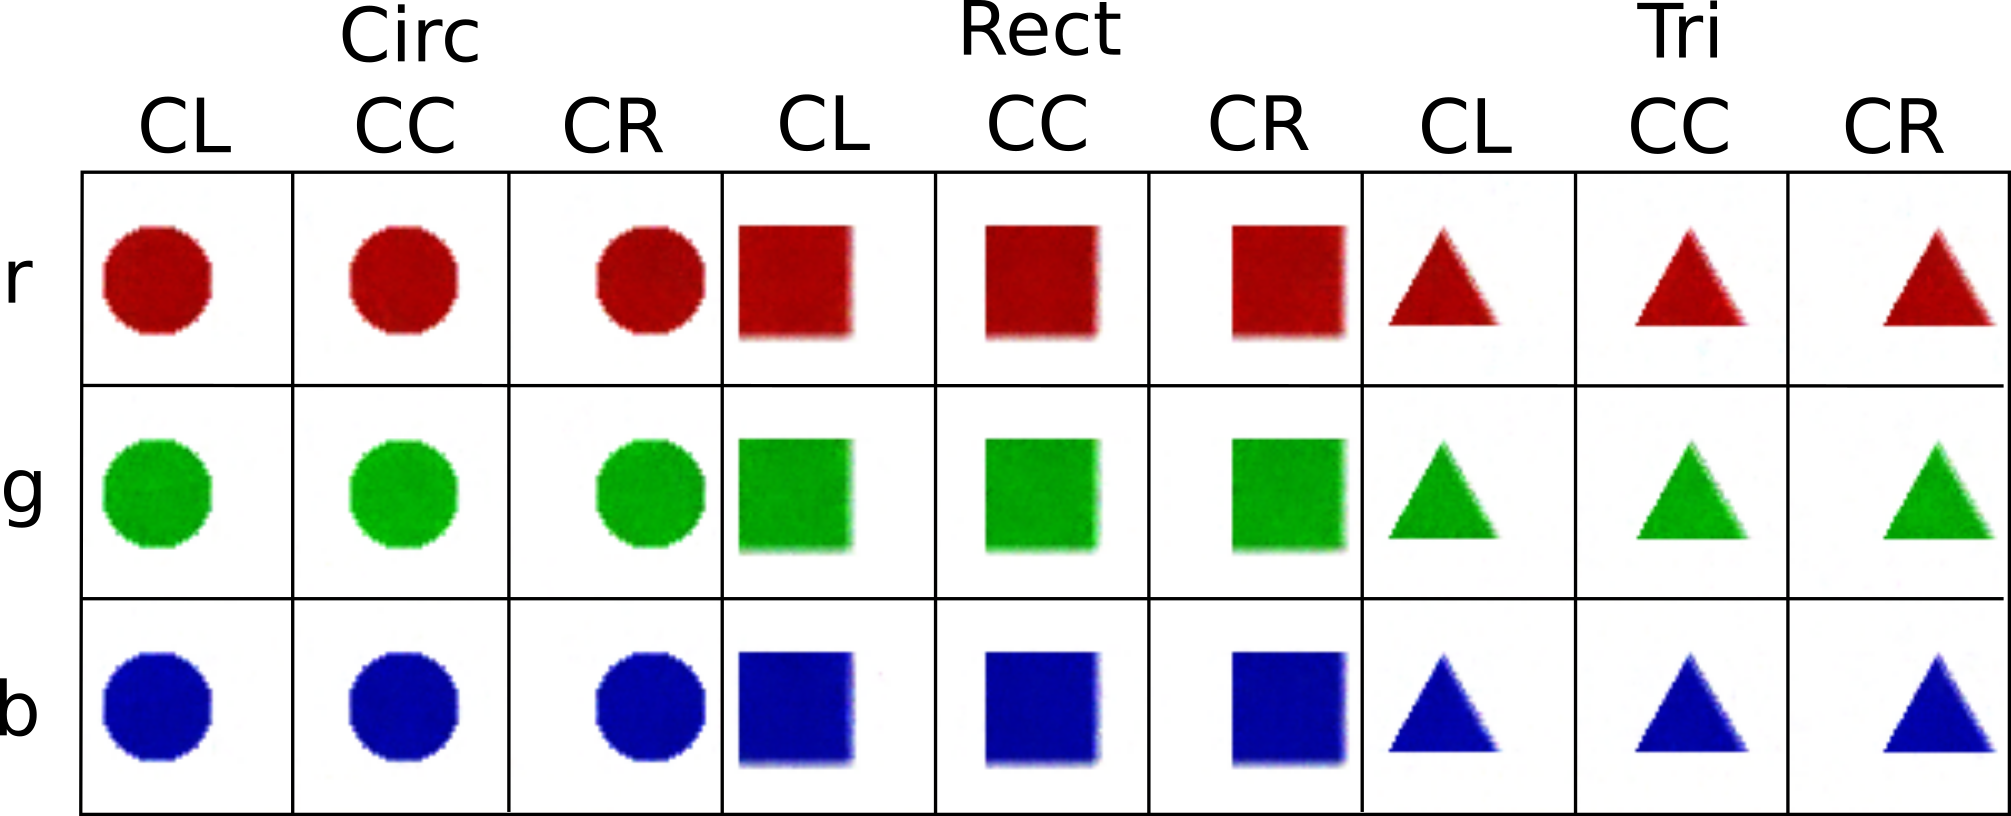
\includegraphics[width=0.75\textwidth]{Figs/shapes/multiword331.png}
%\caption{Experiment 1:  Images generated from descriptions with an embedding size of 200.}
%\label{fig:331multi}
%\end{figure}

Given how well images can be generated from full descriptions, it is unsurpising to see that the MAE has been able to correctly ground the meanings of each of the words of the descriptions. In \autoref{fig:331shapes} it can be seen that each shape is correctly generated into an image for most embedding sizes. It is difficult to specify which embedding size grounds the meanings of each word the best as this is subjective. I would suggest that and embedding size of 296 neurons grounds the meanings of individual words the best, this is due to it producing the most solid circle, rectangle and triangle across all four runs, in my opinion. 

\begin{figure}[h]
\centering
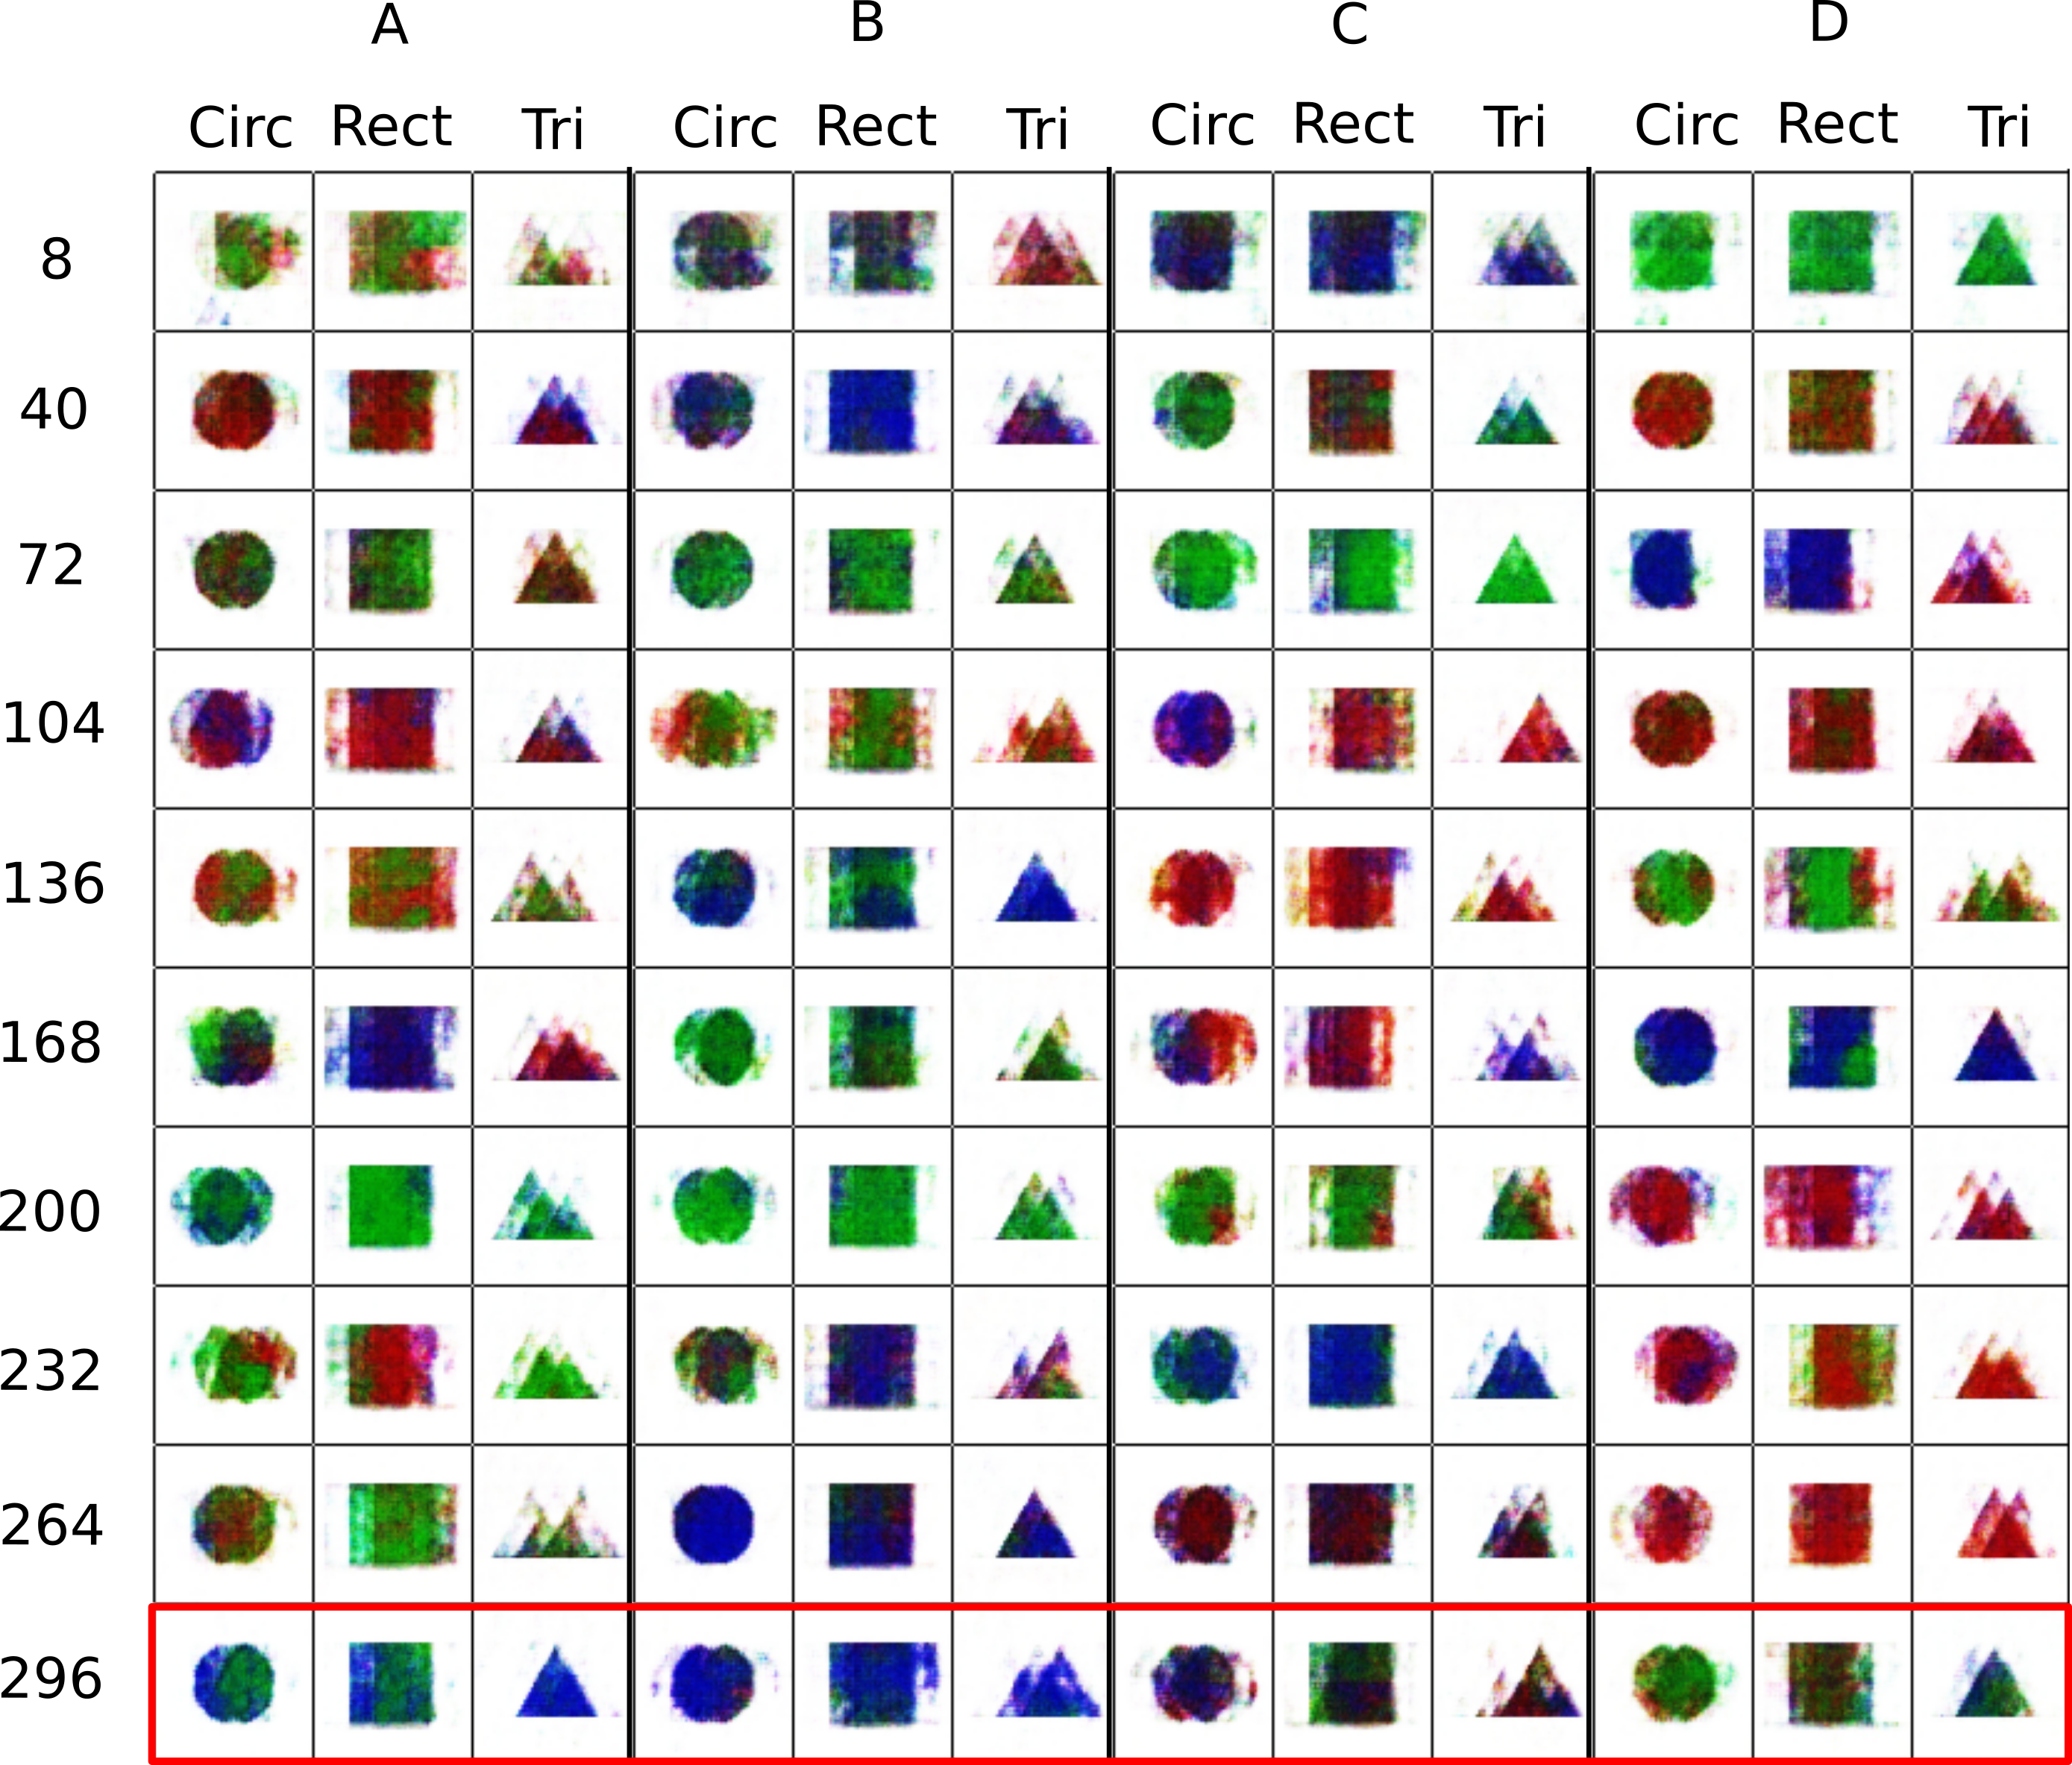
\includegraphics[width=0.75\textwidth]{Figs/shapes/shapes331.png}
\caption{Experiment 1, runs A-D:  Images generated of each shape for different sizes of embedding.}
\label{fig:331shapes}
\end{figure}

The images generated for every word can be found in the suplimental material. As the colour and position are always  correctly learnt across the four runs, they are not shown in the main text.



\paragraph{Description Accuracy}
The MAE gets 100\% accuracy on all descriptions for all testing conditions and all embedding sizes. Accuracy is calculated by counting the number of correctly predicted words and averaging over the entire dataset. For example, given an image described as \textsc{big blue circle left} and the predicted description \textsc{small blue circle left} the accuracy would be 0.75 for that instance as 3 out of 4 words are correctly predicted. A word is considered to be predicted if its neuron's activation is above 0.5. As I am using a sigmoid activation function, the output for each neuron is always between 0 and 1.


\subsubsection{Discussion}
The results of experiment 1 show that the MAE is capable of preforming symbol grounding on this subset of the ArtS dataset. However, it is difficult to make any conclusions about which embedding size gave the best results. Whilst 200 neurons gave the lowest reconstruction error in all testing conditions (see \autoref{tab:res331}), it did not do the best job of grounding the meanings of each word in the descritptions (see \autoref{fig:331shapes}). 

In the next experiment, we will observe how embedding size affects the reconstruction error and symbol grounding of the MAE when a larger variety of sizes for the objects in the images are available.


\newpage
\subsection{Experiment 2}
I will now explore how adding more variety to the data affects the quality of reconstruction. To that end, two new sizes of object are added as seen in \autoref{tab:exp2_data}. 

\begin{table}[ht]
\centering
\begin{tabular}{|c|c|}
\hline
\textbf{Attribute} & \textbf{Description} \\ \hline \hline
\textbf{Shapes} & \textbf{Corners} \\ \hline
Rectangle & 4\\ \hline
Triangle & 3\\ \hline
Circle & 0\\ \hline 

\textbf{Colours} & \textbf{RGB Values}	\\ \hline	
Red & (75,0,0) - (255, 10, 10)\\ \hline
Green  & (0,75,0) - (10, 255, 10)\\ \hline
Blue   & (0,0,75) - (10, 10, 255)\\ \hline


\textbf{Sizes} & 	\textbf{Length/Radius (pixels)} \\ \hline			  
Big    & 32 - 35  \\ \hline
Medium & 22 - 25 \\ \hline
Small  & 12 - 15 \\ \hline 

\textbf{Positions} & \textbf{Object Centre Coordinate}	\\ \hline					  
Centre Left &(22,32)\\ \hline
Centre Centre & (32,32)\\ \hline
Centre Right &(42,32)\\ \hline				
\end{tabular}
\caption{Experiment 2 data subset.}
\label{tab:exp2_data} 
\end{table}



\subsubsection{Results}
\begin{figure}
\centering
\resizebox{0.75\textwidth}{!}{
\begin{tikzpicture}
    \begin{axis}[
     name=plot1,
     axis x line=middle,
     axis y line=middle,
     enlarge y limits=true,
     enlarge x limits=true,
     legend style={at={(0.5,-0.5)}, anchor=north},
     %xmin=0, xmax=2150,
     %ymin=0, ymax=600,
     %width=15cm, height=8cm,     % size of the image
     grid = major,
     grid style={dashed, gray!30},
     ylabel= Total MSE,
     %ytick={0,0.001,0.002,0.003,0.004,0.005,0.006,0.007,0.008,0.009},
     xlabel= (A) Embedding Size,
     %xtick={6,8,10,12,14,16,18,20,22,24,26,28,30,32,34,35,36,37,38,39,40,41,42,43,44,45,46,47,48,49,50,51,52,53,54,55,56},     
	 xlabel near ticks,
	 ylabel near ticks]
         ] 
    ]
    \addplot table[x = size, y = bimodal, col sep = comma]{csvs/333/total333.csv}; 
    \addplot table[x = size, y = words only, col sep = comma]{csvs/333/total333.csv};
    \addplot table[x = size, y = image only, col sep = comma]{csvs/333/total333.csv};    
    \legend{Bimodal, Words Only, Image Only}
    
    \end{axis}
    
    
     \begin{axis}[
     name=plot2,
     at=(plot1.right of south east), 
     anchor=left of south west,
     axis x line=middle,
     axis y line=middle,
     enlarge y limits=true,
     enlarge x limits=true,
     %legend style={at={(1,0.7)}, anchor=north},
     %xmin=0, xmax=2150,
     %ymin=0, ymax=600,
     %width=15cm, height=8cm,     % size of the image
     grid = major,
     grid style={dashed, gray!30},
     ylabel= Image MSE,
     %ytick={0,0.001,0.002,0.003,0.004,0.005,0.006,0.007,0.008,0.009},
     xlabel= (B) Embedding Size,
     %xtick={6,8,10,12,14,16,18,20,22,24,26,28,30,32,34,35,36,37,38,39,40,41,42,43,44,45,46,47,48,49,50,51,52,53,54,55,56},     
     xlabel near ticks,
	 ylabel near ticks]
         ] 
    ]
    \addplot table[x = size, y = bimodal, col sep = comma]{csvs/333/image333.csv}; 
    \addplot table[x = size, y = words only, col sep = comma]{csvs/333/image333.csv};
    \addplot table[x = size, y = image only, col sep = comma]{csvs/333/image333.csv}; 
       
    %\legend{Bimodal, Words Only, Image Only}
    \end{axis}
    
	
    
    \begin{axis}[
     name=plot3,
     at=(plot2.below south west),
     anchor=above north west,
     axis x line=middle,
     axis y line=middle,
     enlarge y limits=true,
     enlarge x limits=true,
     %legend style={at={(1,0.7)}, anchor=north},
     %xmin=0, xmax=2150,
     %ymin=0, ymax=600,
     %width=15cm, height=8cm,     % size of the image
     grid = major,
     grid style={dashed, gray!30},
     ylabel= Word MSE,
     %ytick={0,0.001,0.002,0.003,0.004,0.005,0.006,0.007,0.008,0.009},
     xlabel= (C) Embedding Size,
     %xtick={6,8,10,12,14,16,18,20,22,24,26,28,30,32,34,35,36,37,38,39,40,41,42,43,44,45,46,47,48,49,50,51,52,53,54,55,56},     
     xlabel near ticks,
	 ylabel near ticks]
         ] 
    ]
    \addplot table[x = size, y = bimodal, col sep = comma]{csvs/333/word333.csv}; 
    \addplot table[x = size, y = words only, col sep = comma]{csvs/333/word333.csv};
    \addplot table[x = size, y = image only, col sep = comma]{csvs/333/word333.csv};    
    %\legend{Bimodal, Words Only, Image Only}
    \end{axis}
    

\end{tikzpicture}
}
\caption{Experiment 2: MSE for reconstruction of images and descriptions under different testing conditions. (A) shows the total MSE, (B) shows the MSE of the image output and (C) shows the MSE of the word output.}
\label{fig:graph333}
\end{figure}

Once again we see that the majority of error comes from the image reconstruction loss by comparing the scales of \autoref{fig:graph333} (B) and (C). The description reconstruction error is larger and less stable with respect to the embedding size than in experiment 1. However it still remains very small with a scale of $10^{-4}$ vs $10^{-5}$.

Interestingly, we see that increasing the embedding size seems to have a positive effect on image reconstruction error under all testing conditions, though this is not a large improvement in the Words Only testing condition. \autoref{tab:res333} highlights this, with the best total error occuring for an embedding size of 296 neurons in all three testing conditions. 
Comparing this to the results of experiment 1, where 200 neurons was the best embedding size with respect to reconstruction error, it is possible that as the data becomes more complex, the extra neurons allow for better represention of the multimodal data.

\begin{table}
\centering
	\begin{tabular}{|c|c|c|c|}
	\hline
	Size & 	Bimodal & 	Image Only 	& 	Words Only \\ \hline
8	&	6.65	$\mypm$	0.20	&	6.68	$\mypm$	0.30	&	7.37	$\mypm$	0.30	\\ \hline
40	&	5.38	$\mypm$	0.10	&	5.27	$\mypm$	0.30	&	5.66	$\mypm$	0.10	\\ \hline
72	&	5.57	$\mypm$	0.50	&	6.67	$\mypm$	1.90	&	5.90	$\mypm$	0.50	\\ \hline
104	&	5.04	$\mypm$	0.20	&	4.69	$\mypm$	0.20	&	5.52	$\mypm$	0.20	\\ \hline
136	&	4.89	$\mypm$	0.20	&	4.57	$\mypm$	0.20	&	5.53	$\mypm$	0.10	\\ \hline
168	&	4.91	$\mypm$	0.20	&	4.50	$\mypm$	0.20	&	5.51	$\mypm$	0.10	\\ \hline
200	&	4.70	$\mypm$	0.20	&	4.60	$\mypm$	0.70	&	5.47	$\mypm$	0.10	\\ \hline
232	&	4.91	$\mypm$	0.30	&	4.53	$\mypm$	0.30	&	5.66	$\mypm$	0.20	\\ \hline
264	&	4.64	$\mypm$	0.20	&	4.28	$\mypm$	0.20	&	5.46	$\mypm$	0.10	\\ \hline
296	&	\textbf{4.41}	$\mypm$	0.10	&	\textbf{4.19}	$\mypm$	0.30	&	\textbf{5.44}	$\mypm$	0.10	\\ \hline

	\end{tabular}
\caption{Experiment 2:  Total MSE for different embedding sizes. An Embedding Size of 296 neurons provides the minimum reconstruction error. (All values are $\times10^{-3}$)}
\label{tab:res333}
\end{table}


\paragraph{Image Generation}

\begin{figure}[h]
\centering
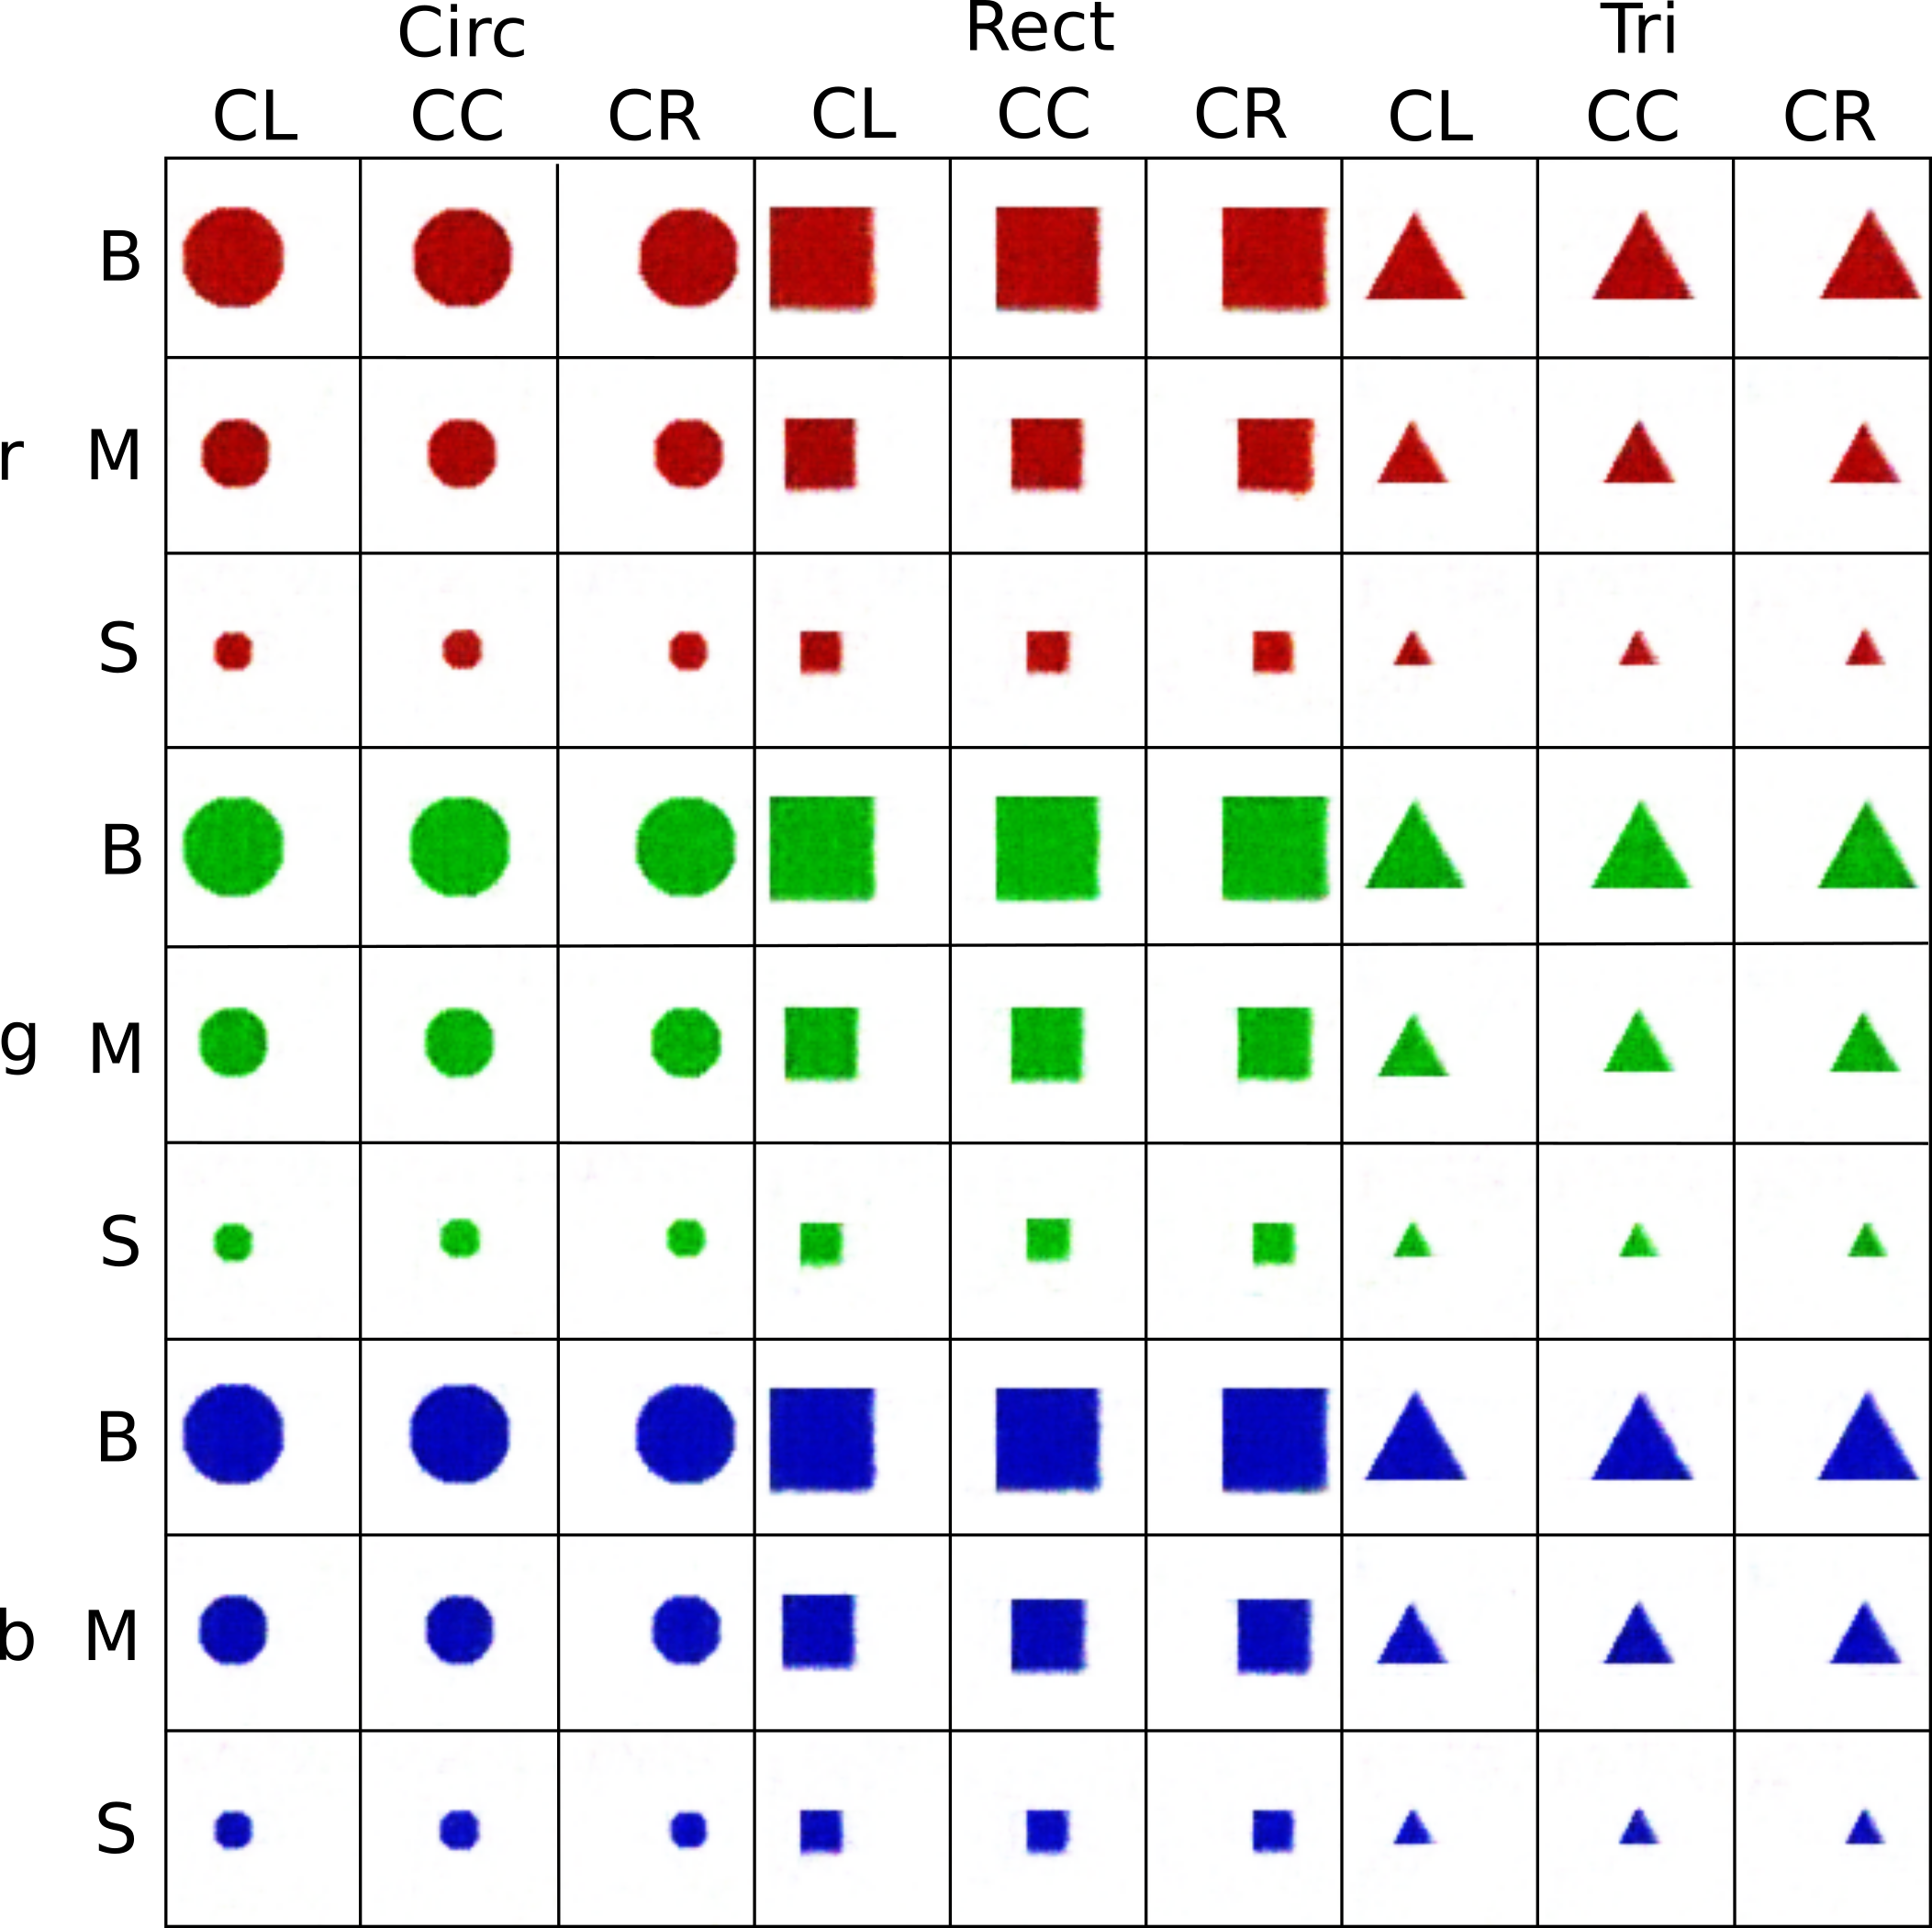
\includegraphics[width=0.5\textwidth]{Figs/shapes/multiword333.png}
\caption{Experiment 2: Images generated from descriptions with an embedding size of 296 neurons.}
\label{fig:333multi}
\end{figure}

Generating images from full descriptions remains effective as seen in \autoref{fig:333multi}.
With the addition of the extra sizes, generation of images from a single word has become significantly poorer. However, it is still clear that at least some of the words have been succefully grounded. Particularly, the meaning of colours and positions are correctly learnt, with images of distinct colours and positions being generated as seen in \autoref{fig:333single}. 

There is also a clear releationship between the three sizes, shown by the generation of the most coloured pixels for the word \textsc{Big}, fewer for \textsc{Medium} and the least for \textsc{Small}.

\begin{figure}[h]
\centering
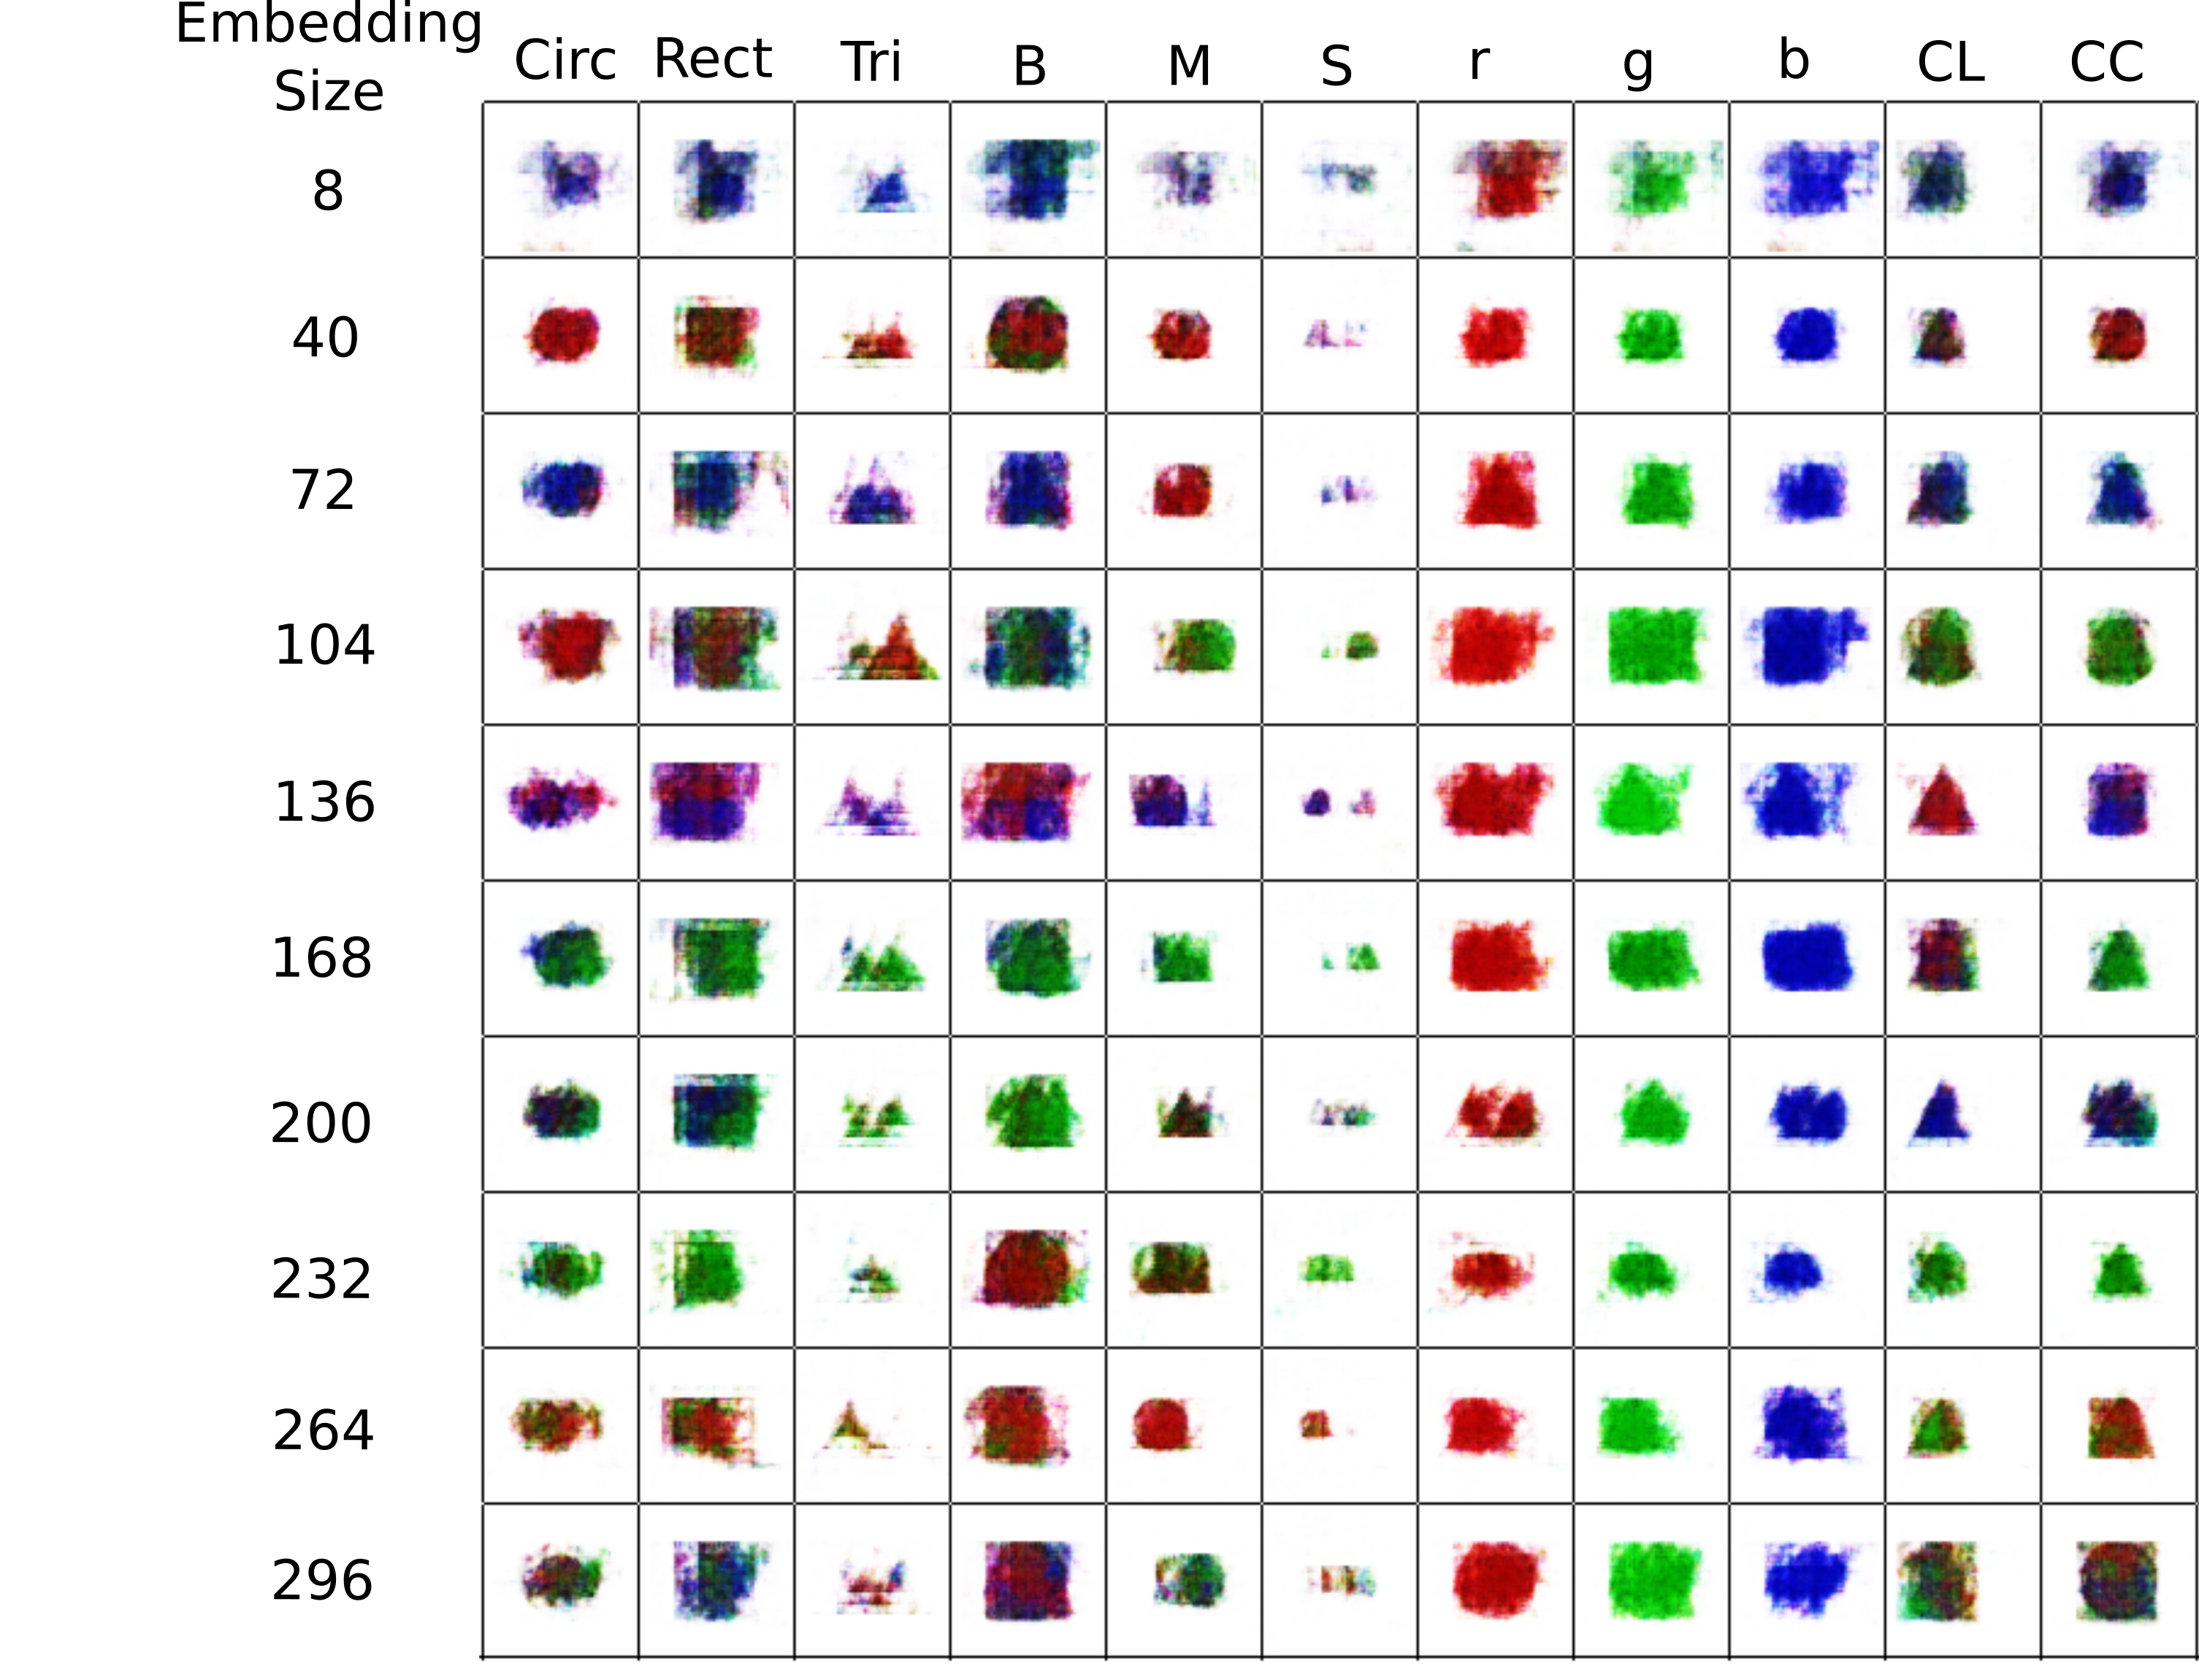
\includegraphics[width=0.75\textwidth]{Figs/shapes/singlelabel333A.png}
\caption{Experiment 2 run A: Images generated of each word for different embedding sizes.}
\label{fig:333single}
\end{figure} 

The quality of the shapes being generated from the words \textsc{Circle}, \textsc{Rectangle} and \textsc{Triangle} has suffered the most. However, there is a clear difference between the three shapes and they do show properties of the shapes they are supposed to be. The \textsc{Circle} is generally more round than either of the other shapes. The \textsc{Rectangle} has approxiamtely 4 sides at right angles to one and other, though it is significantly more ``fuzzy'' than in experiment 1. The \textsc{Triangle} appears triangular, however, for most embedding sizes there appear to be multiple triangles being drawn, this could signify a confusion about where to draw the triangle. I reason that this is the case as in \autoref{fig:2word333} the triangle is significantly more solid when a position is specified. 


\begin{figure}[h]
\centering
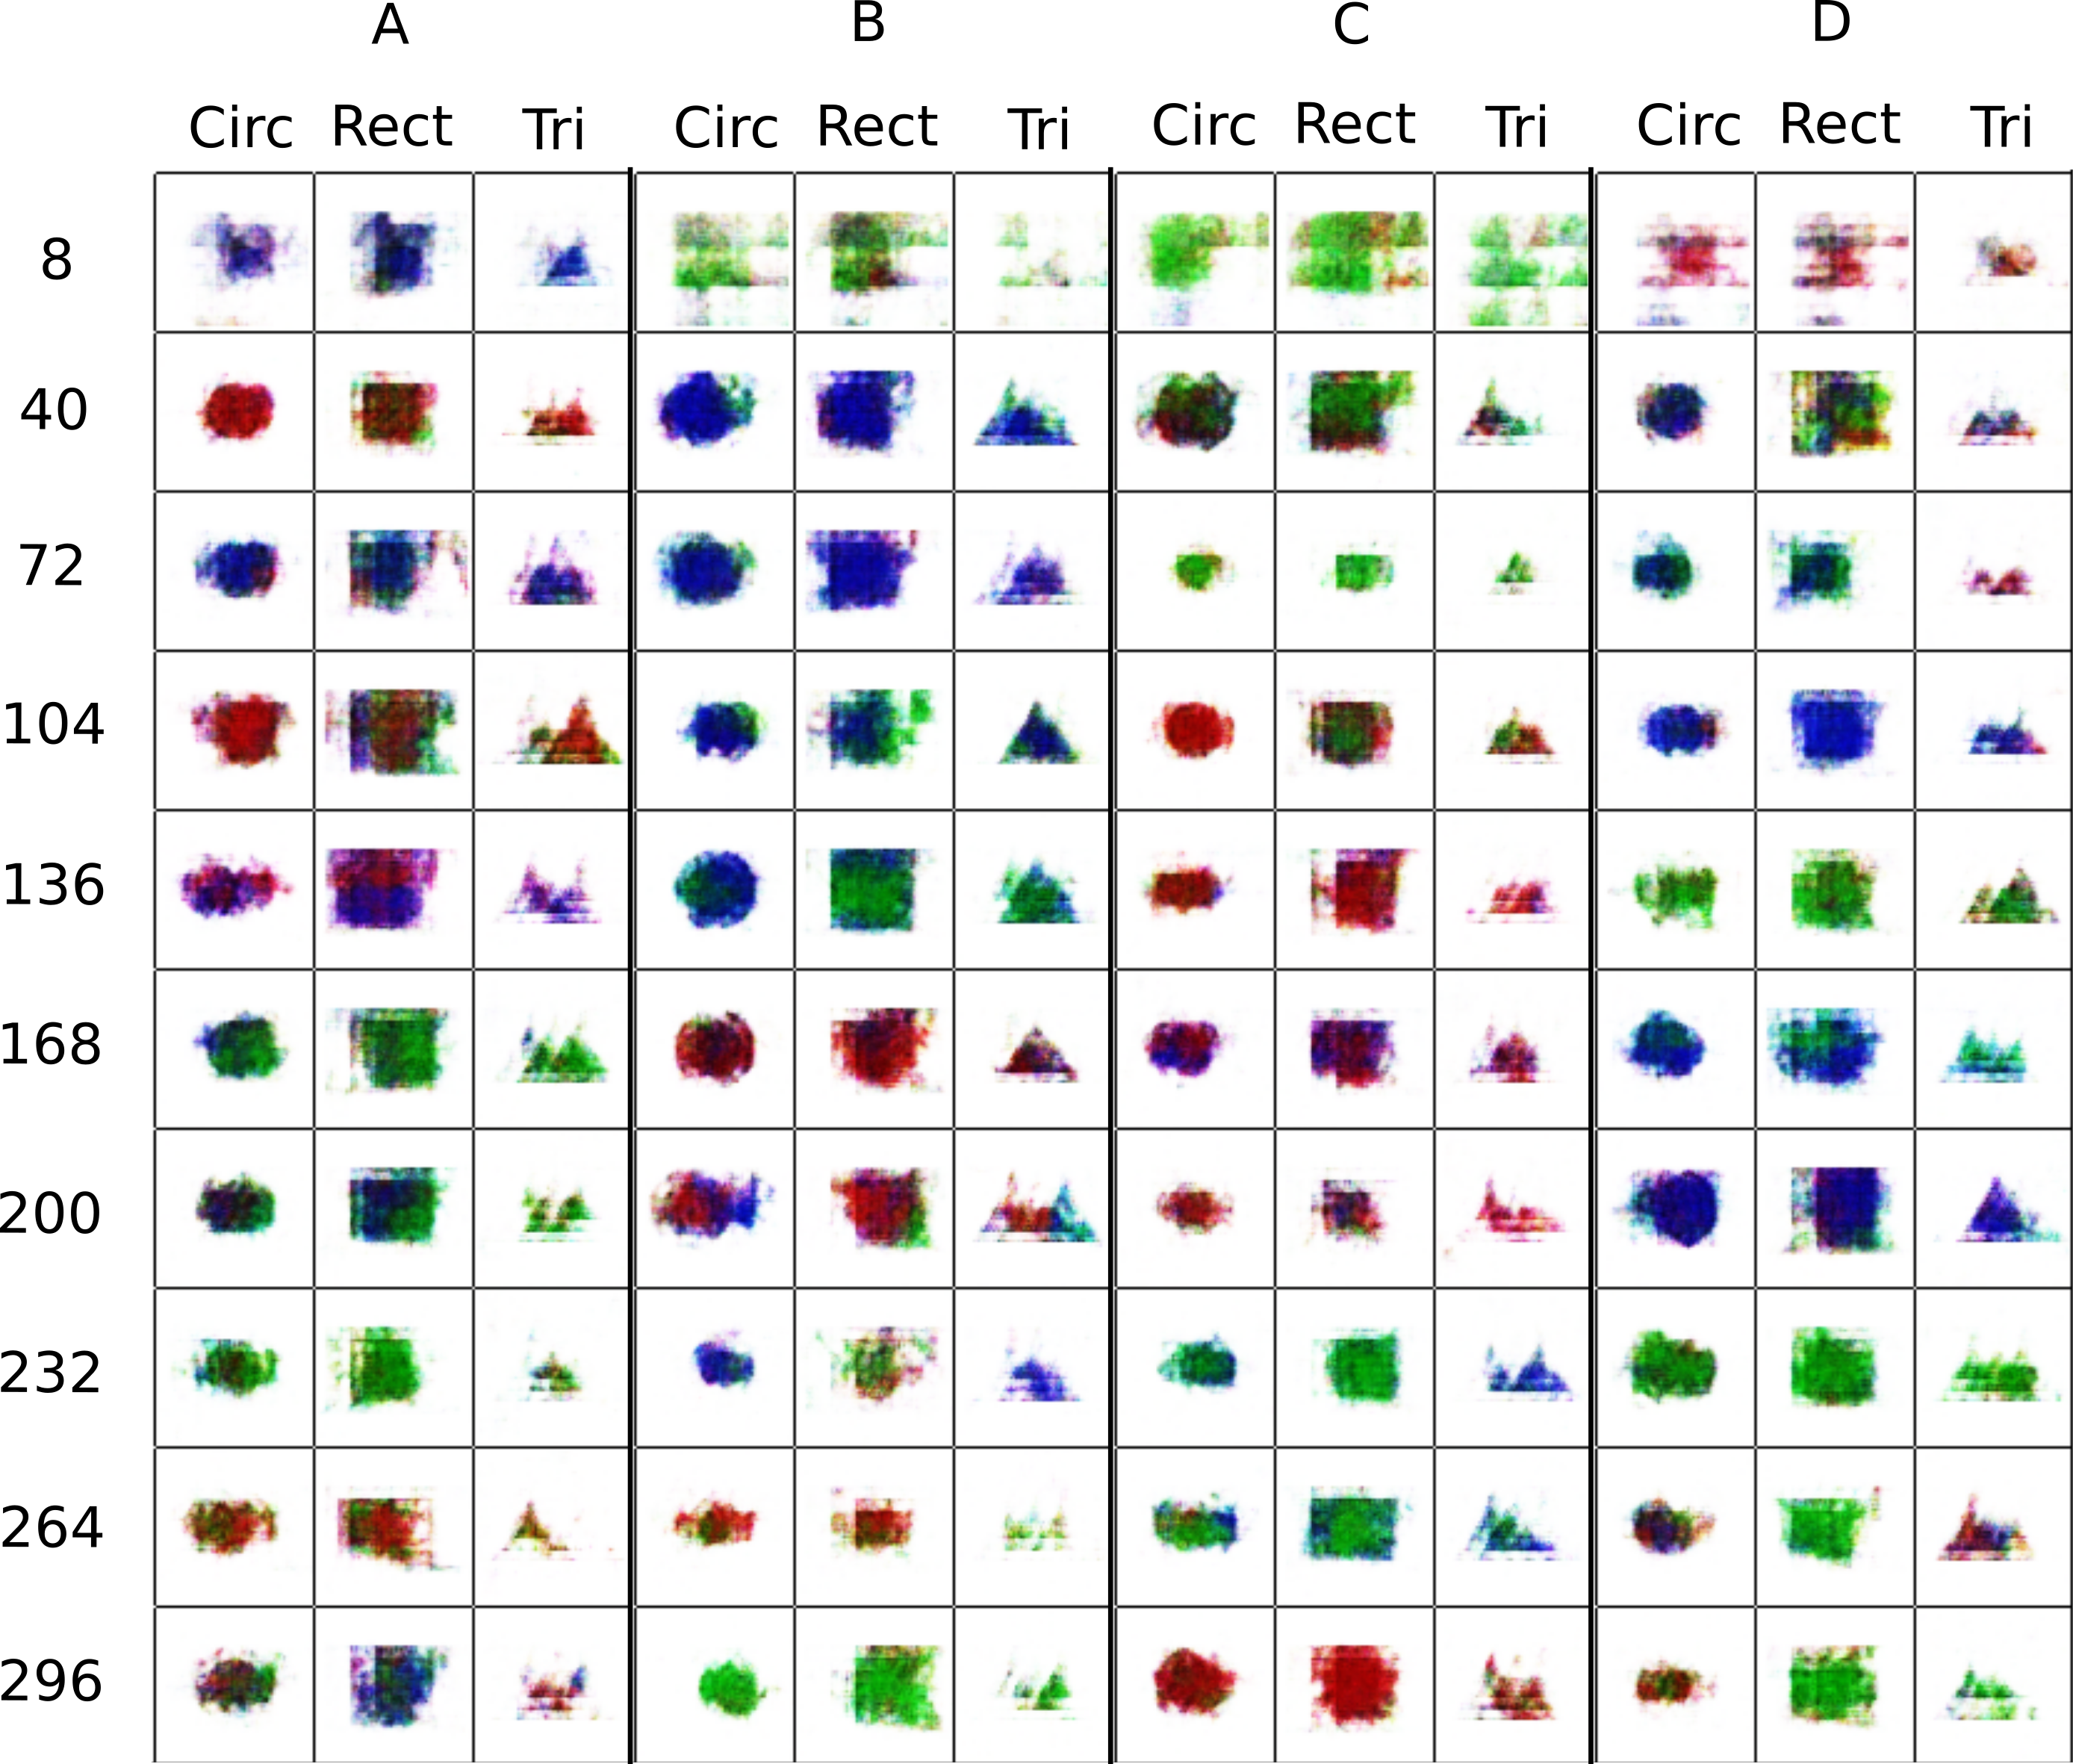
\includegraphics[width=0.75\textwidth]{Figs/shapes/shapes333.png}
\caption{Experiment 2, runs A-D:  Images generated of each shape for different emedding sizes.}
\label{fig:shapes333}
\end{figure}

Whilst an embedding size of 136 neurons disentangled the meanings of \textsc{Circle}, \textsc{Rectangle} and \textsc{Triangle} in run B of experiment 2, this result was not consistent across all four runs (or for any other embedding size) as seen in \autoref{fig:shapes333}. This indicates that the weight initialisation and data selection have an effect on whether the MAE can learn the meanings of the shape names (\textsc{Circle}, \textsc{Rectangle} and \textsc{Triangle}) when additional object sizes are added to the training data.


\begin{figure}[h]
\centering
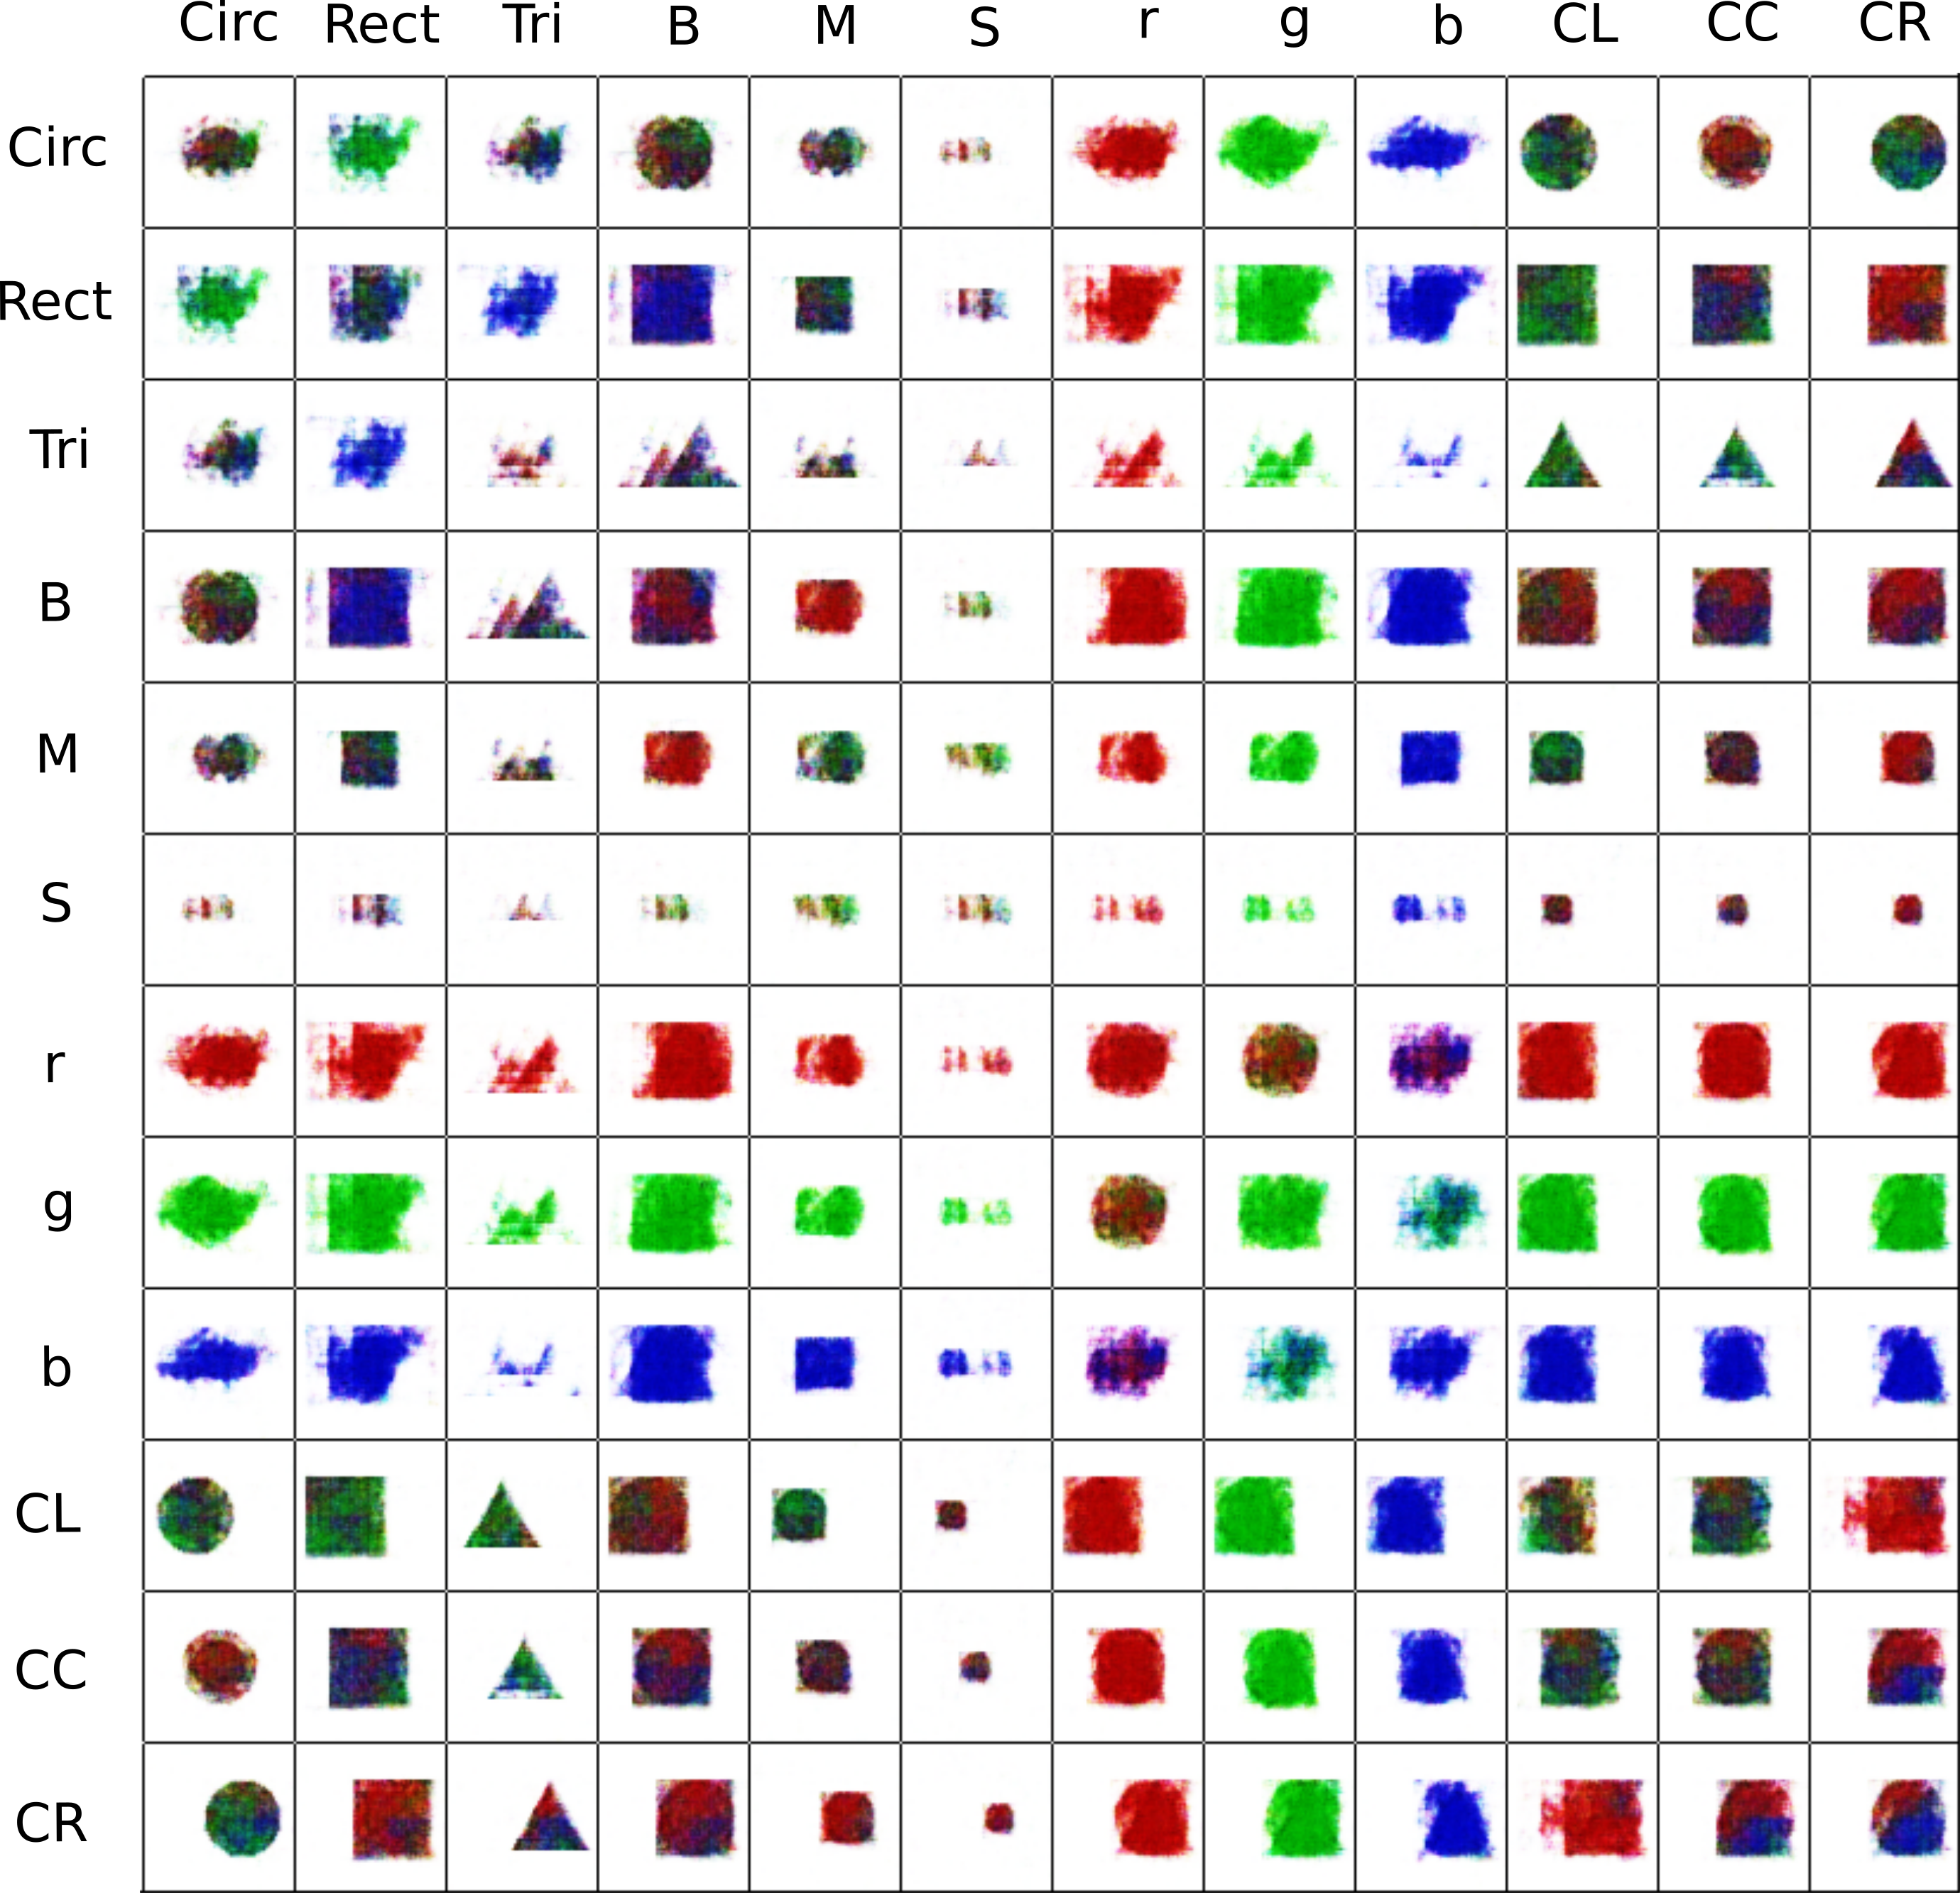
\includegraphics[width=0.75\textwidth]{Figs/shapes/2word333A.png}
\caption{Experiment 2, run A:  Images generated using word pairs using an embedding size of 296 neurons.}
\label{fig:2word333}
\end{figure}

Another way to inspect the quality of the learnt embedding is to provide pairs of words to the MAE and observe what it generates as output. \autoref{fig:2word333} shows the output of the MAE trained in run A of experiment 2 (runs B-D can be found in \autoref{appendix:B} with an embedding size of 296 neurons. Here we see clearly that the MAE is correctly generating images from the words \textsc{Circle}, \textsc{Rectangle} and \textsc{Triangle} as well as the other words in its ``vocabulary''. The diagonal of \autoref{fig:2word333} is the equivalent of the bottom row (296) of \autoref{fig:333single}. The addition of a second word allows for the correct generation of the three shapes in different positions and sizes, suggesting that when only the shape is provided as input, the MAE does not know where to draw the object or how big to draw it. By adding a second word and removing some uncertainty, the output of the MAE is much more defined. This is a particularly strong result in the case of when a position is provided in conjuction with either a shape, size or colour. 


\paragraph{Description Accuracy}
Even with the added complexity of the additional sizes, the MAE gets 100\% accuracy in all testing conditions for all embedding sizes. 


\subsubsection{Discussion}

Increasing the number of variable attributes in the dataset, i.e. adding the extra sizes, has had a negative affect on the ability of the MAE to ground the meanings of each of the words in the descriptions. This is highlighted when the results of experiments 1 and 2 are seen side by side as in \autoref{fig:shapes333v331}.

\begin{figure}[h]
\centering
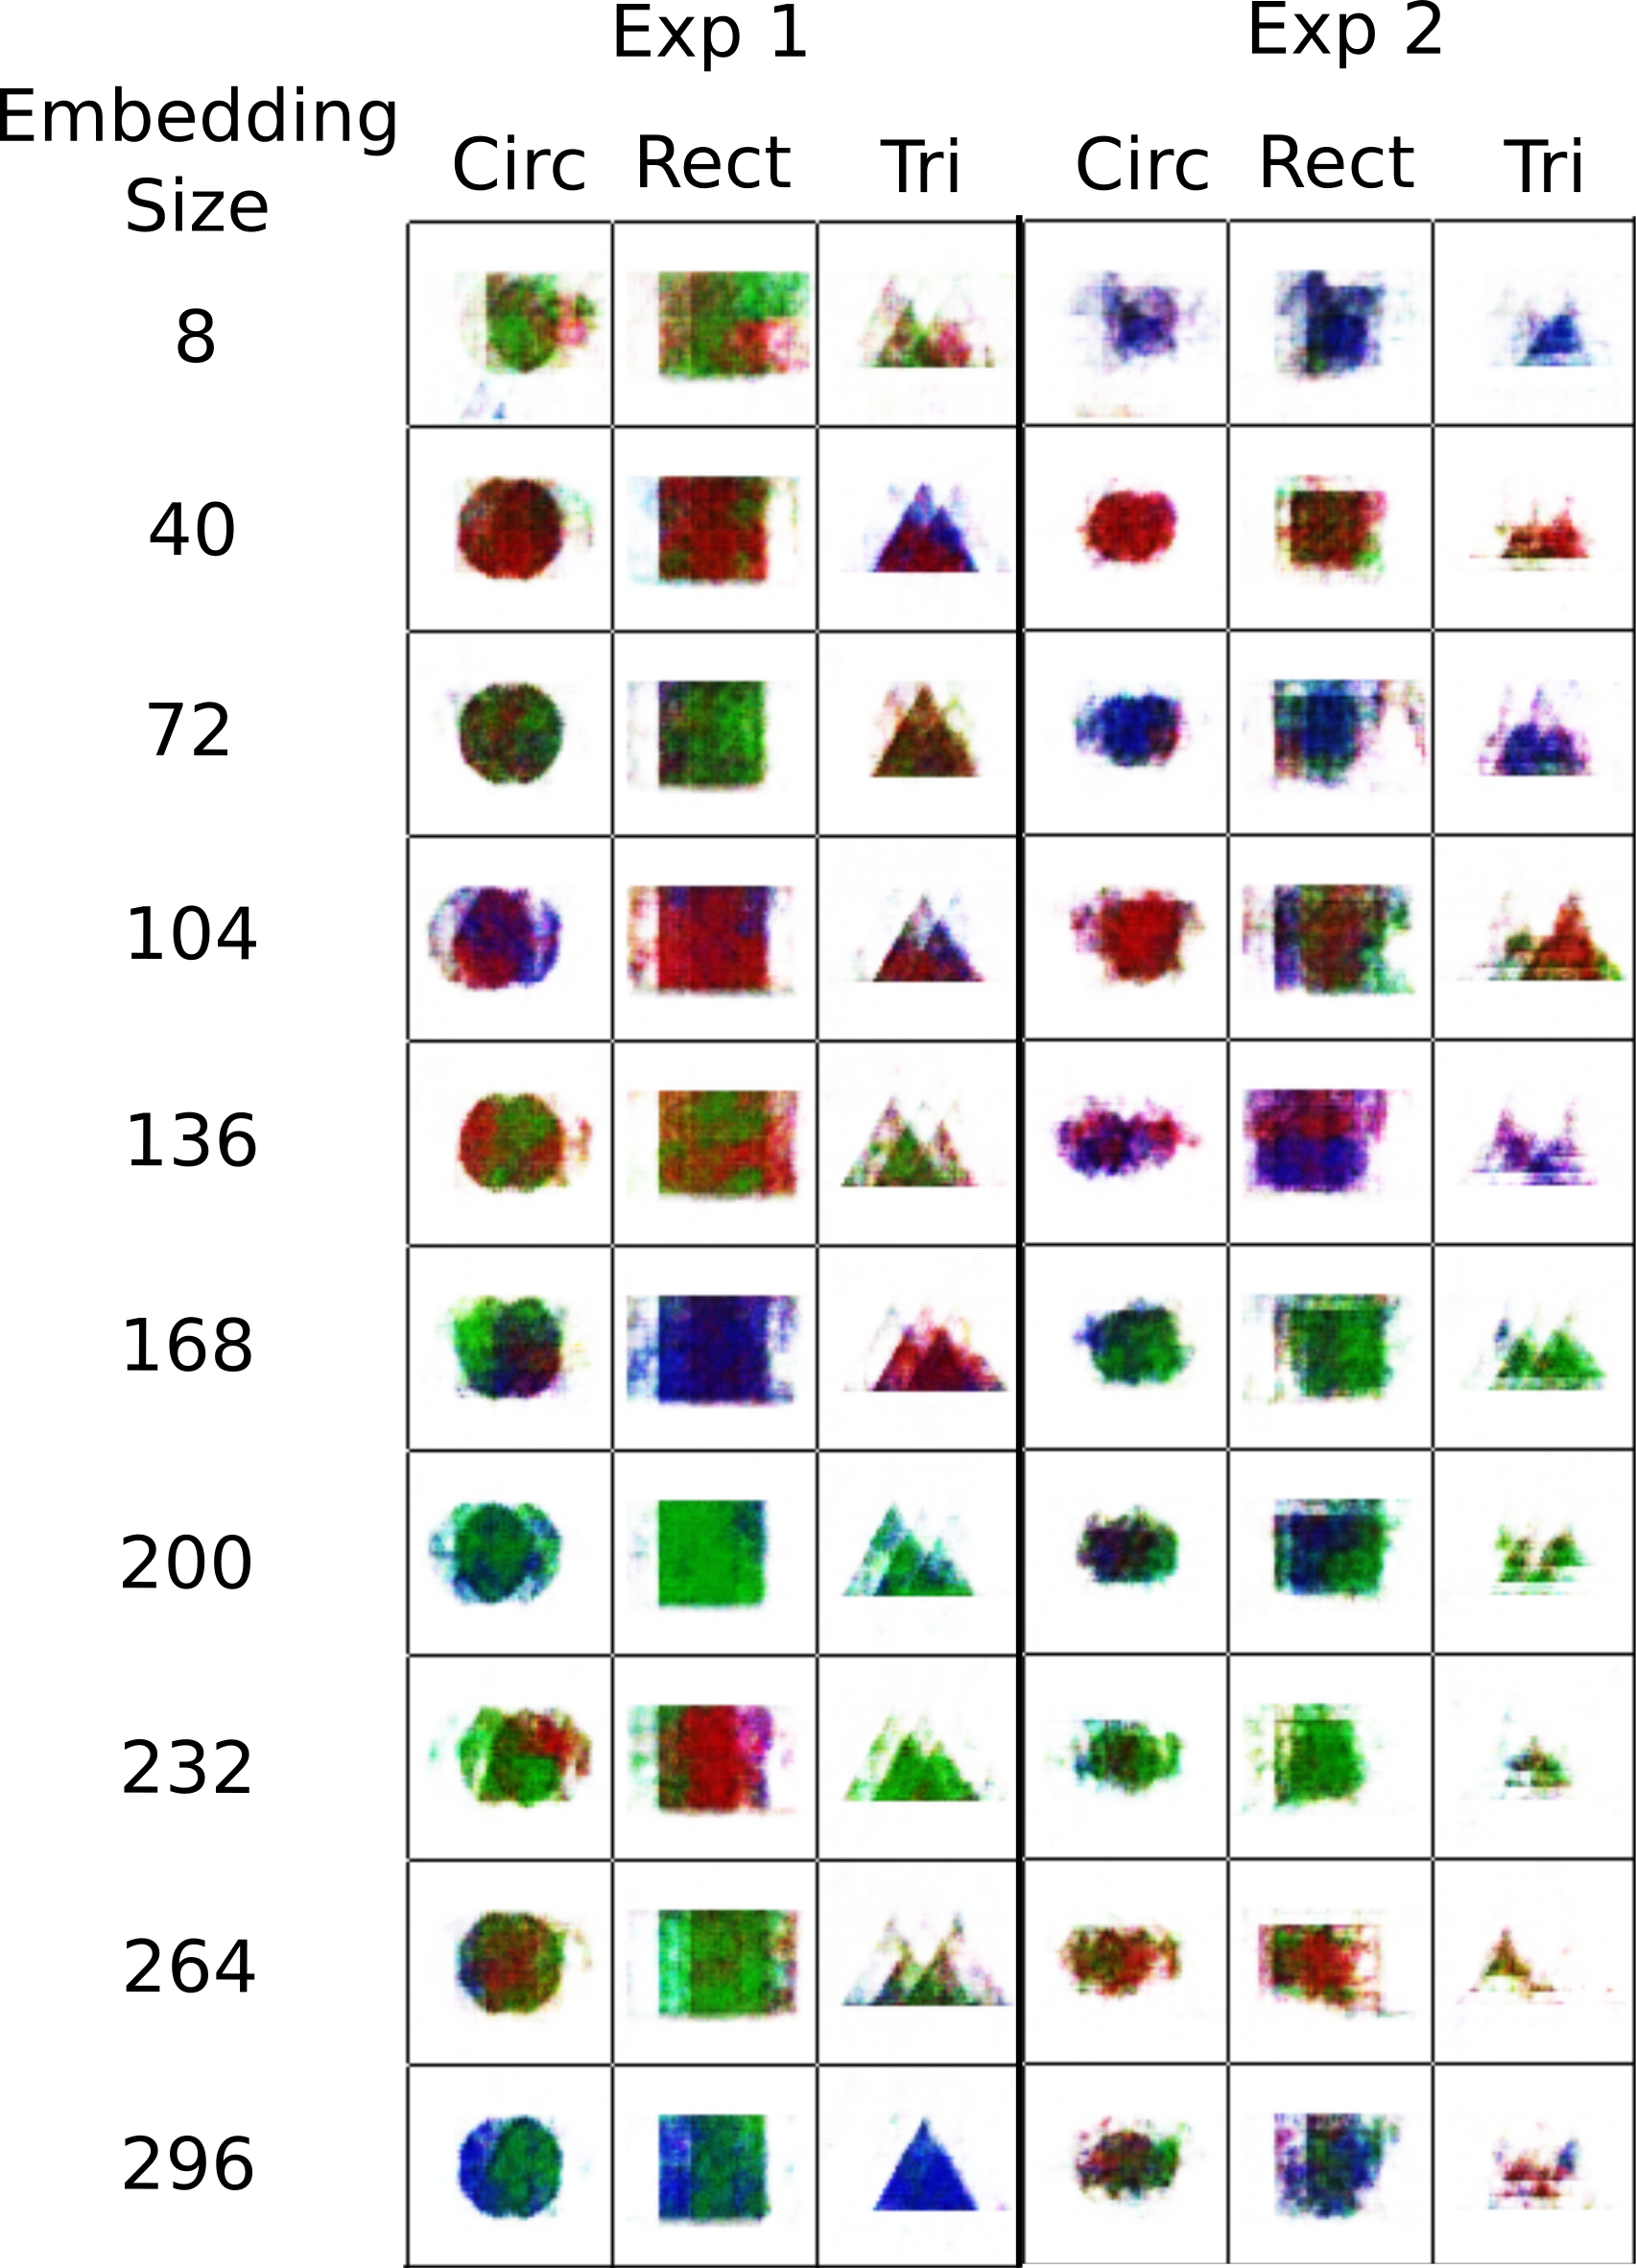
\includegraphics[width=0.4\textwidth]{Figs/shapes/shapes331v333.png}
\caption{Images generated of each shape for different sizes of embedding using the MAEs trained in experiments 1 and 2 run A.}
\label{fig:shapes333v331}
\end{figure} %This issue could likely be solved by the addition of more examples per object.
However, the MAE remains able to accurately generate images from full descriptions (see \autoref{fig:333multi}). 
An embedding size of 296 neurons gave the all around best performance in experiment 2 and performed the best at symbol grounding in experiment 1, therefore it will be used for the later experiments.

\newpage
\subsection{Experiment 3}
This experiment adds further vairety to the data, adding an additional 6 positions as seen in \autoref{tab:exp3_data}. In this experiment, we will also observe how incrementally learning these new properties affects the quality of the generated outputs as well as the bidirectional grounding of the different words from the descriptions and visual attributes of the images. 

Incremental learning is performed by transfering the weights learned in the previous experiments and then performing further training on the datasubset of experiment 3. By comparing the quality of the output from a MAE trained starting from random weights, with the MAEs pretrained in experiments 1 and 2 (after they train on the data for experiment 3), I will answer the fundamental question of whether, having knowledge of the meaning of a subset of words and visual attributes, aids the learning of new words and image attributes.

To make this a fair comparison, the MAE which is initialised with random weights will be trained for 100 epochs so that the total number of epochs of training that each MAE receives is equal. I.e. either 50 epochs pretraining and 50 epochs training or 100 epochs of training.


\begin{table}[h]
\centering
\begin{tabular}{|c|c|}
\hline
\textbf{Attribute} & \textbf{Description} \\ \hline \hline
\textbf{Shapes} & \textbf{Corners} \\ \hline
Rectangle & 4\\ \hline
Triangle & 3\\ \hline
Circle & 0\\ \hline 

\textbf{Colours} & \textbf{RGB Values}	\\ \hline	
Red & (75,0,0) - (255, 10, 10)\\ \hline
Green  & (0,75,0) - (10, 255, 10)\\ \hline
Blue   & (0,0,75) - (10, 10, 255)\\ \hline

\textbf{Sizes} & 	\textbf{Length/Radius (pixels)} \\ \hline			  
Big    & 32 - 35  \\ \hline
Medium & 22 - 25 \\ \hline
Small  & 12 - 15 \\ \hline 

\textbf{Positions} & \textbf{Object Centre Coordinate}	\\ \hline					  
Top Left & (22,42)\\ \hline	
Top Centre & (32,42)\\ \hline
Top Right & (42,42)\\ \hline
Centre Left &(22,32)\\ \hline
Centre & (32,32)\\ \hline
Centre Right &(42,32)\\ \hline
Bottom Left & (22,22)\\ \hline
Bottom Centre & (22,42)\\ \hline
Bottom Right & (42,22)\\ \hline				
\end{tabular}
\caption{Experiment 2 data subset.}
\label{tab:exp3_data} 
\end{table}

Unlike in the previous two experiments, the embedding size will be fixed to 296 neurons as this gave the best performance in experiment 2 in terms of error.

The different initialisation schemes will be referred to as: Random: randomly initialised weights, Exp1: initialisation with the weights trained during experiment 1 and Exp2: initialisation with the weights trained during experiment 2.

\subsubsection{Results}
Using the pretrained weights from experiment 1 as a starting point for experiment 3 leads to the lowest reconstruction error as seen in \autoref{tab:res339}. The lower reconstruction error during testing does not translate to improved symbol grounding.


\begin{table}[h!]
\centering
	\begin{tabular}{|c|c|c|c|}
	\hline
	Initialisation & 	Bimodal & 	Image Only 	& 	Words Only \\ \hline
	Random	&	\textbf{3.97}	$\mypm$	0.41	&	22.73	$\mypm$	35.14	&	\textbf{4.09}	$\mypm$	0.27\\ \hline
	Exp 1 	&	5.29	$\mypm$	0.47	&	6.69	$\mypm$	3.48	&	5.78	$\mypm$	0.33	\\ \hline
	Exp 2 	&	5.33	$\mypm$	0.31	&	\textbf{5.06}	$\mypm$	0.38	&	5.75	$\mypm$	0.24	\\ \hline

	\end{tabular}
\caption{Experiment 3: Total MSE for different weight initialisations. (All values are $\times10^{-3}$)}
\label{tab:res339}
\end{table}


\paragraph{Image Generation}
It is not feasable to show every combination of shape, colour, size and position, so in \autoref{fig:339multi} a selection of these combinations are shown.

\begin{figure}[h]
\centering
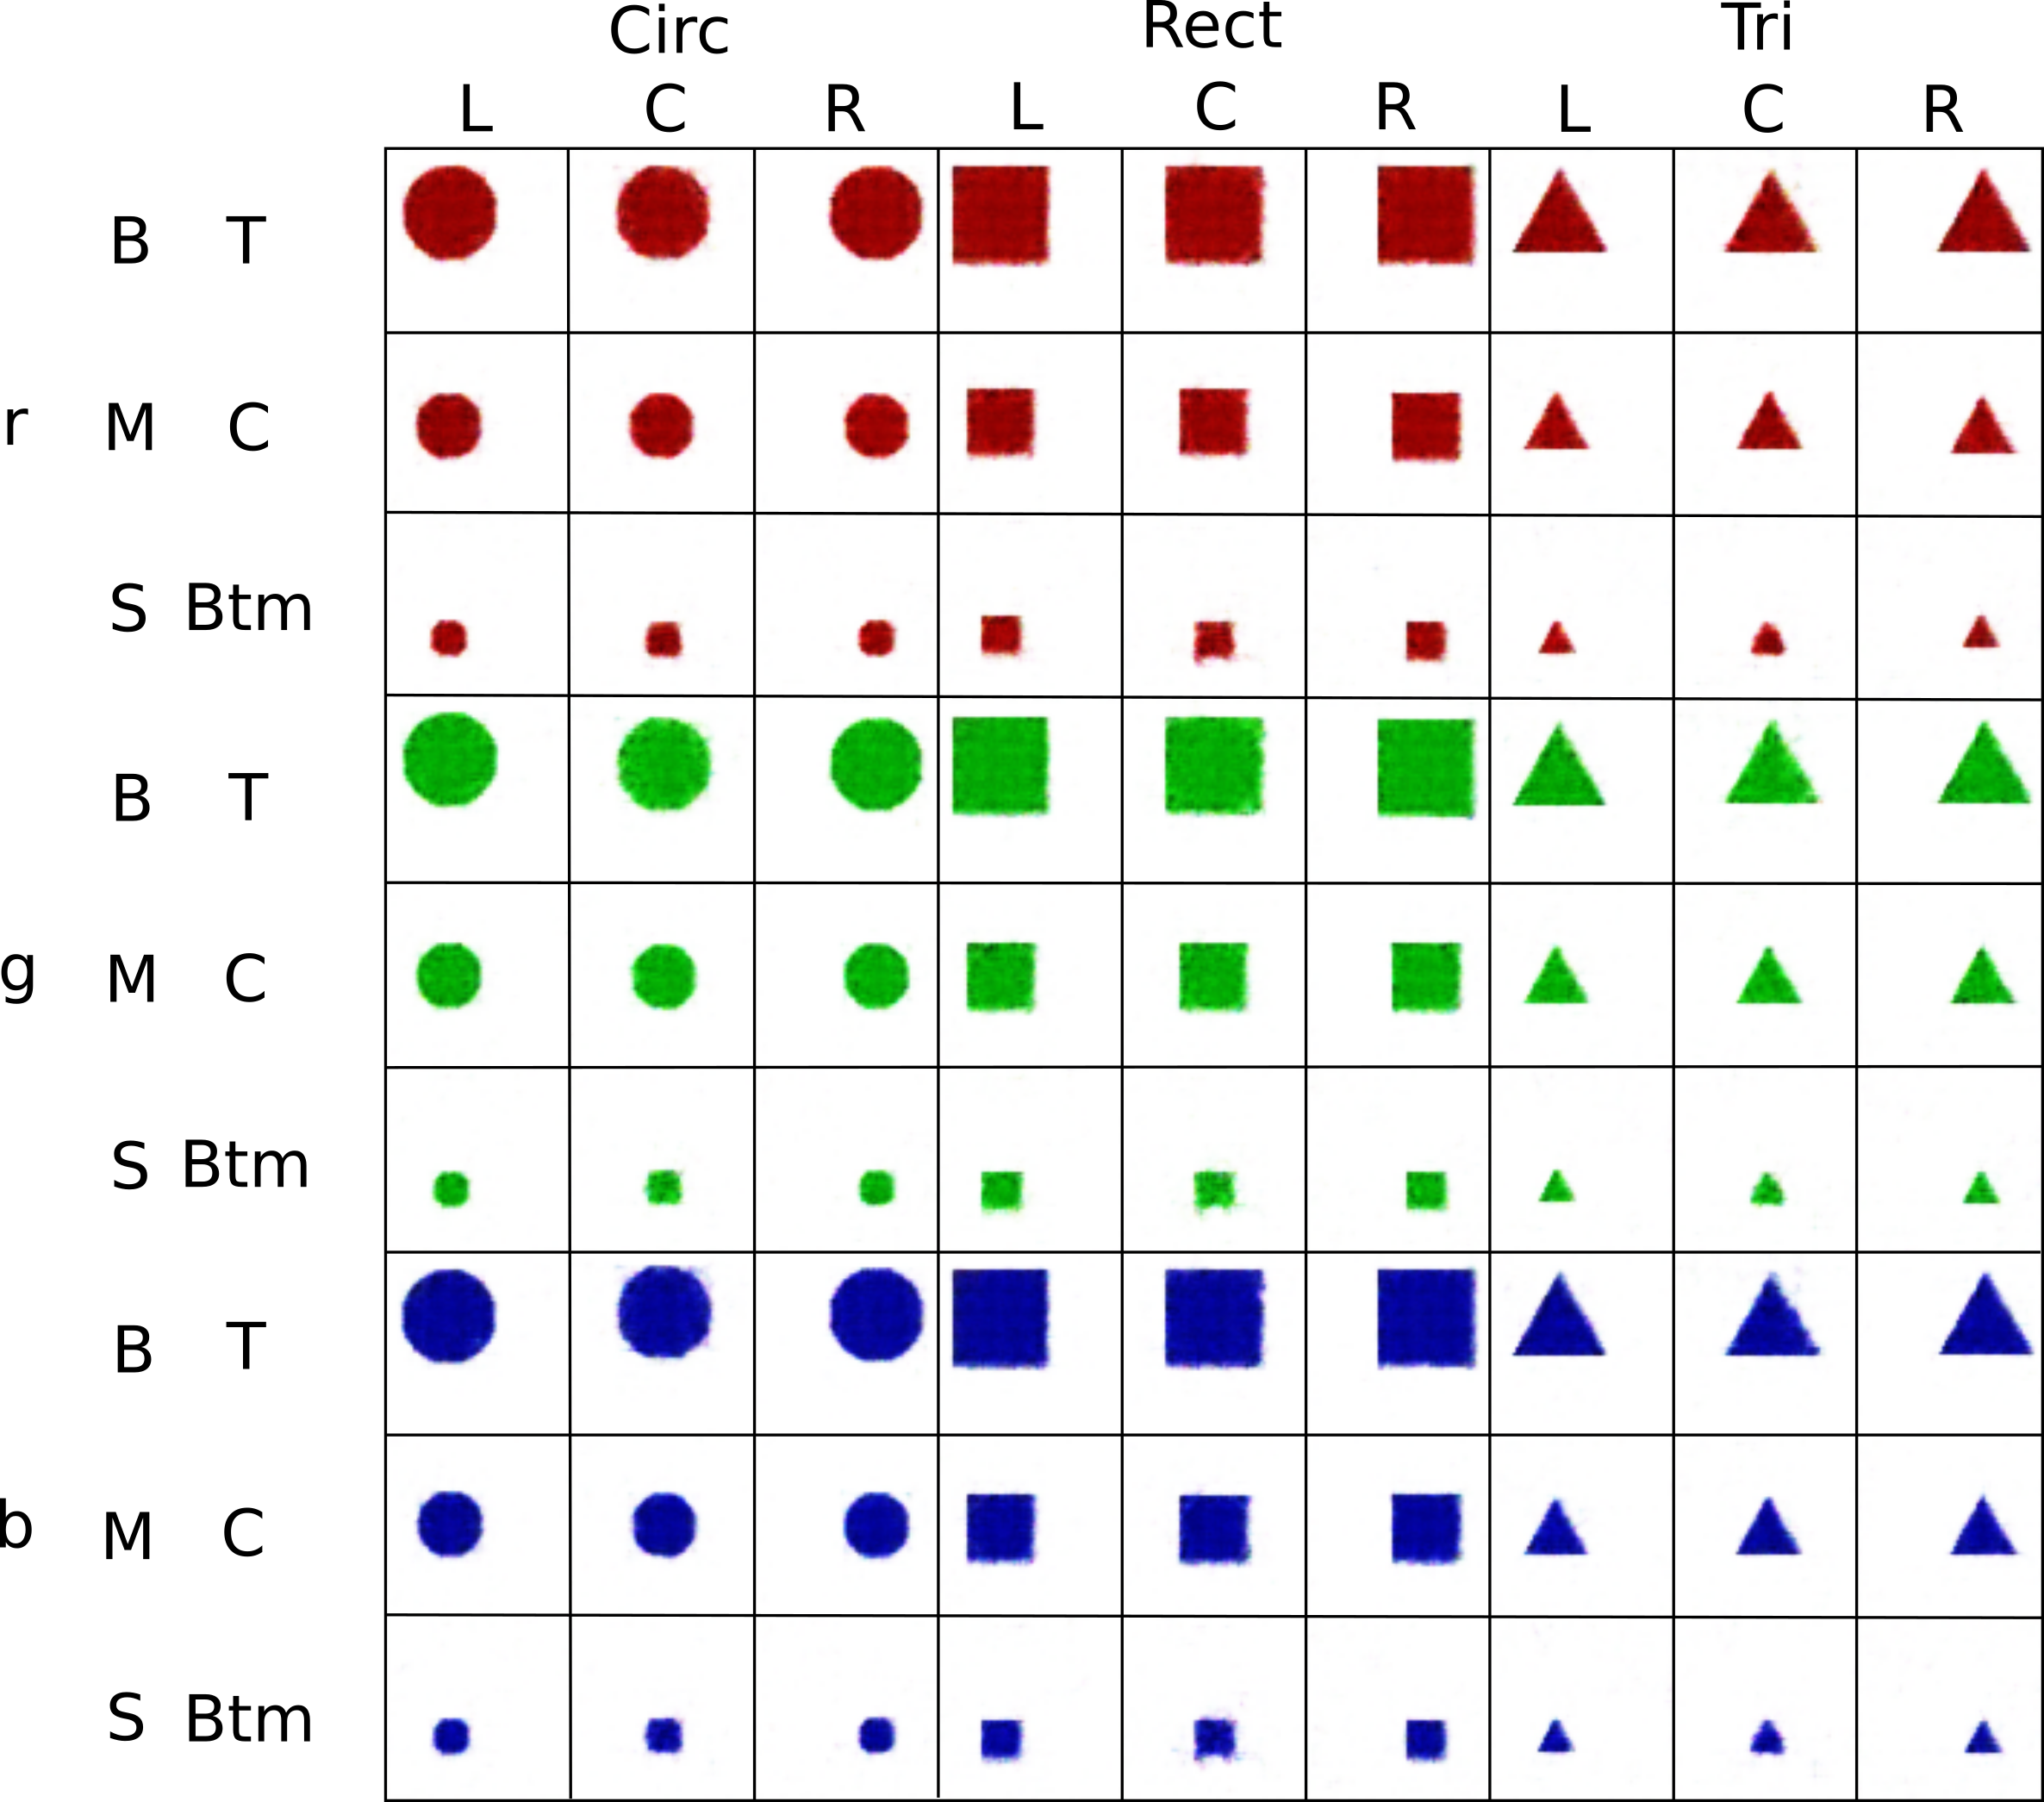
\includegraphics[width=0.625\textwidth]{Figs/shapes/multiword339.png}
\caption{Experiment 3, run A: Images generated from descriptions, starting training from randomly initialised weights.}
\label{fig:339multi}
\end{figure}

The addition of new positions has had an effect on the quality of the images generated from descriptions by the MAE. The images have become blurrier compared to images generated in previous experiments. However they are still easily recognisable as matching their descriptions.

When only given a single word as input, as in \autoref{fig:339single}, the MAE is not able to correctly generate any of the shapes (\textit{Circle}, \textit{Rectangle},\textit{Triangle}). Unlike in experiment 2, where the words \textsc{Circle}, \textsc{Rectangle} and\textsc{Triangle} lead to the generation of visual attributes which match these words, in experiment 3 it is unclear that these visual attributes can be seen.
The colours are all correctly generated and again, the sizes show a clear relation with the most pixels being coloured for \textsc{big} matching the visual attribute \textit{big} and the least for \textsc{small} matching the visual attribute \textit{small}.

\begin{figure}[h]
\centering
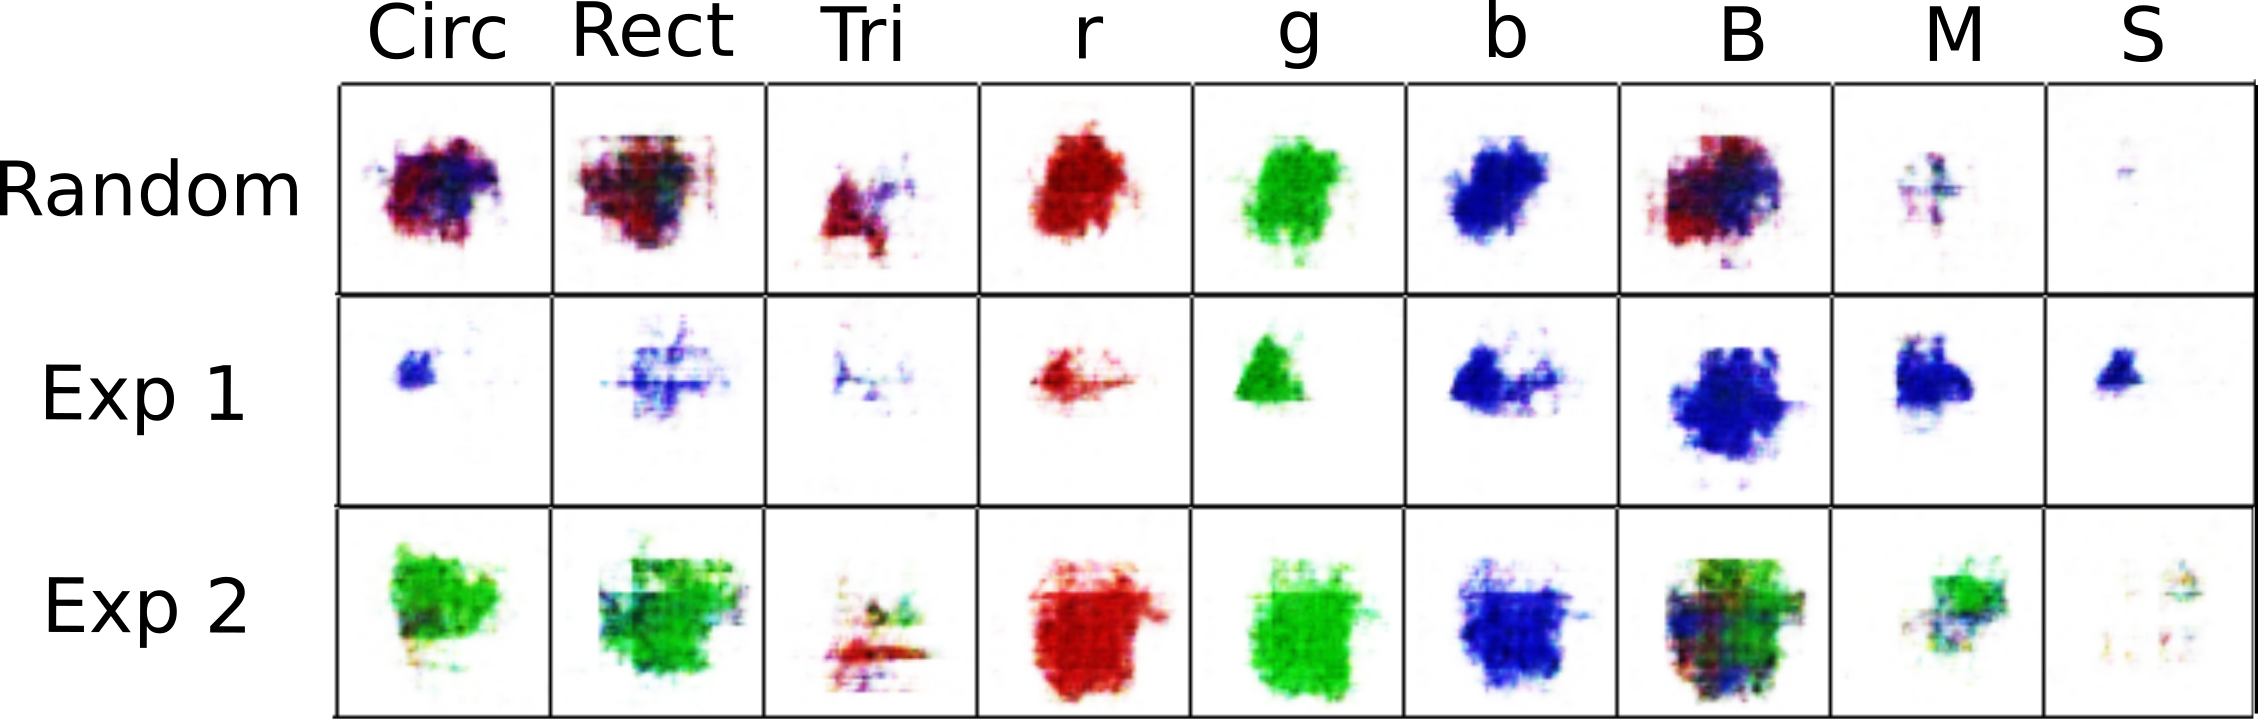
\includegraphics[width=0.75\textwidth]{Figs/shapes/singlelabel339.png}
\caption{Experiment 3, run A: Images generated from shape, colour and size words for different weight initialisation conditions.}
\label{fig:339single}
\end{figure}

The new positions are correctly learnt with a clear distinction between positions on the top, centre and bottom as well as left, centre and right and their combinations (e.g. bottom right) as seen in \autoref{fig:339single_pos}.

\begin{figure}[h]
\centering
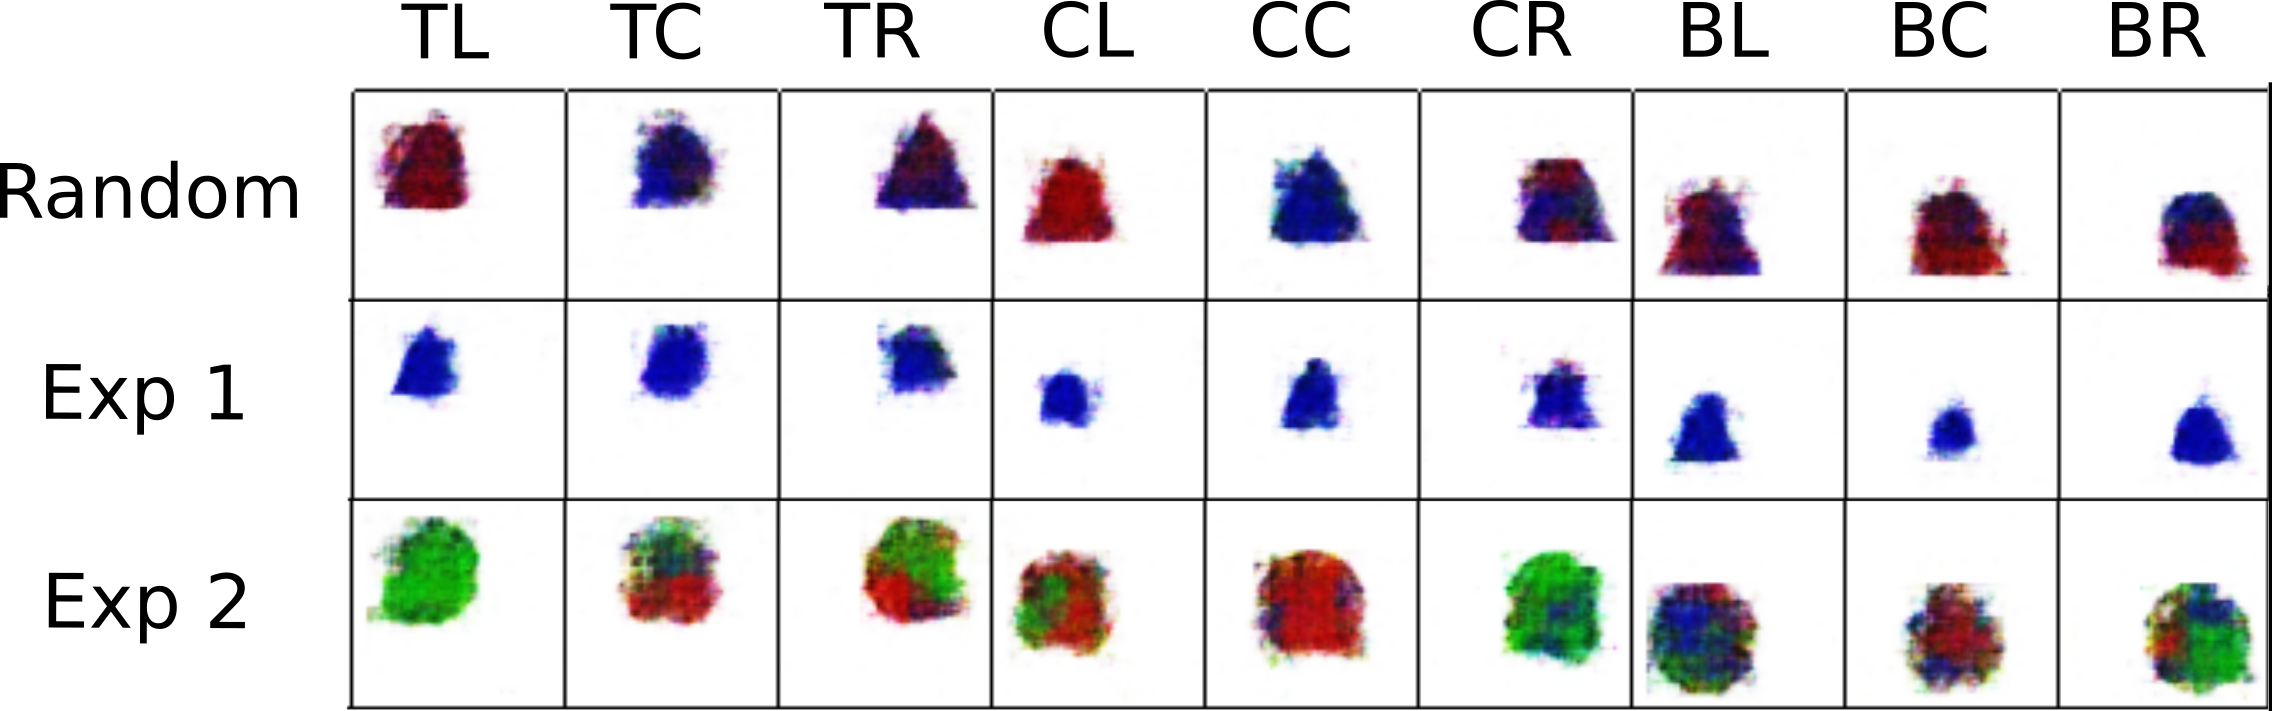
\includegraphics[width=0.75\textwidth]{Figs/shapes/singlelabel339_pos.png}
\caption{Experiment 3, run A: Images generated from each position word for different weight initialisation conditions.}
\label{fig:339single_pos}
\end{figure}


As in experiment 2, the addition of a second word as input, leads to better reconstruction of the visual attributes with which they are associated. \autoref{fig:2word339} shows a comparison of the three different weight initialisations after training. It is clear in all three cases that the MAE learns to correctly ground the words \textsc{Circle}, \textsc{Rectangle} and\textsc{Triangle}. However, in the case of initialising with weights from experiment 1, the pretraining results in a worse performance than random weights.
\begin{figure}[h]
\centering
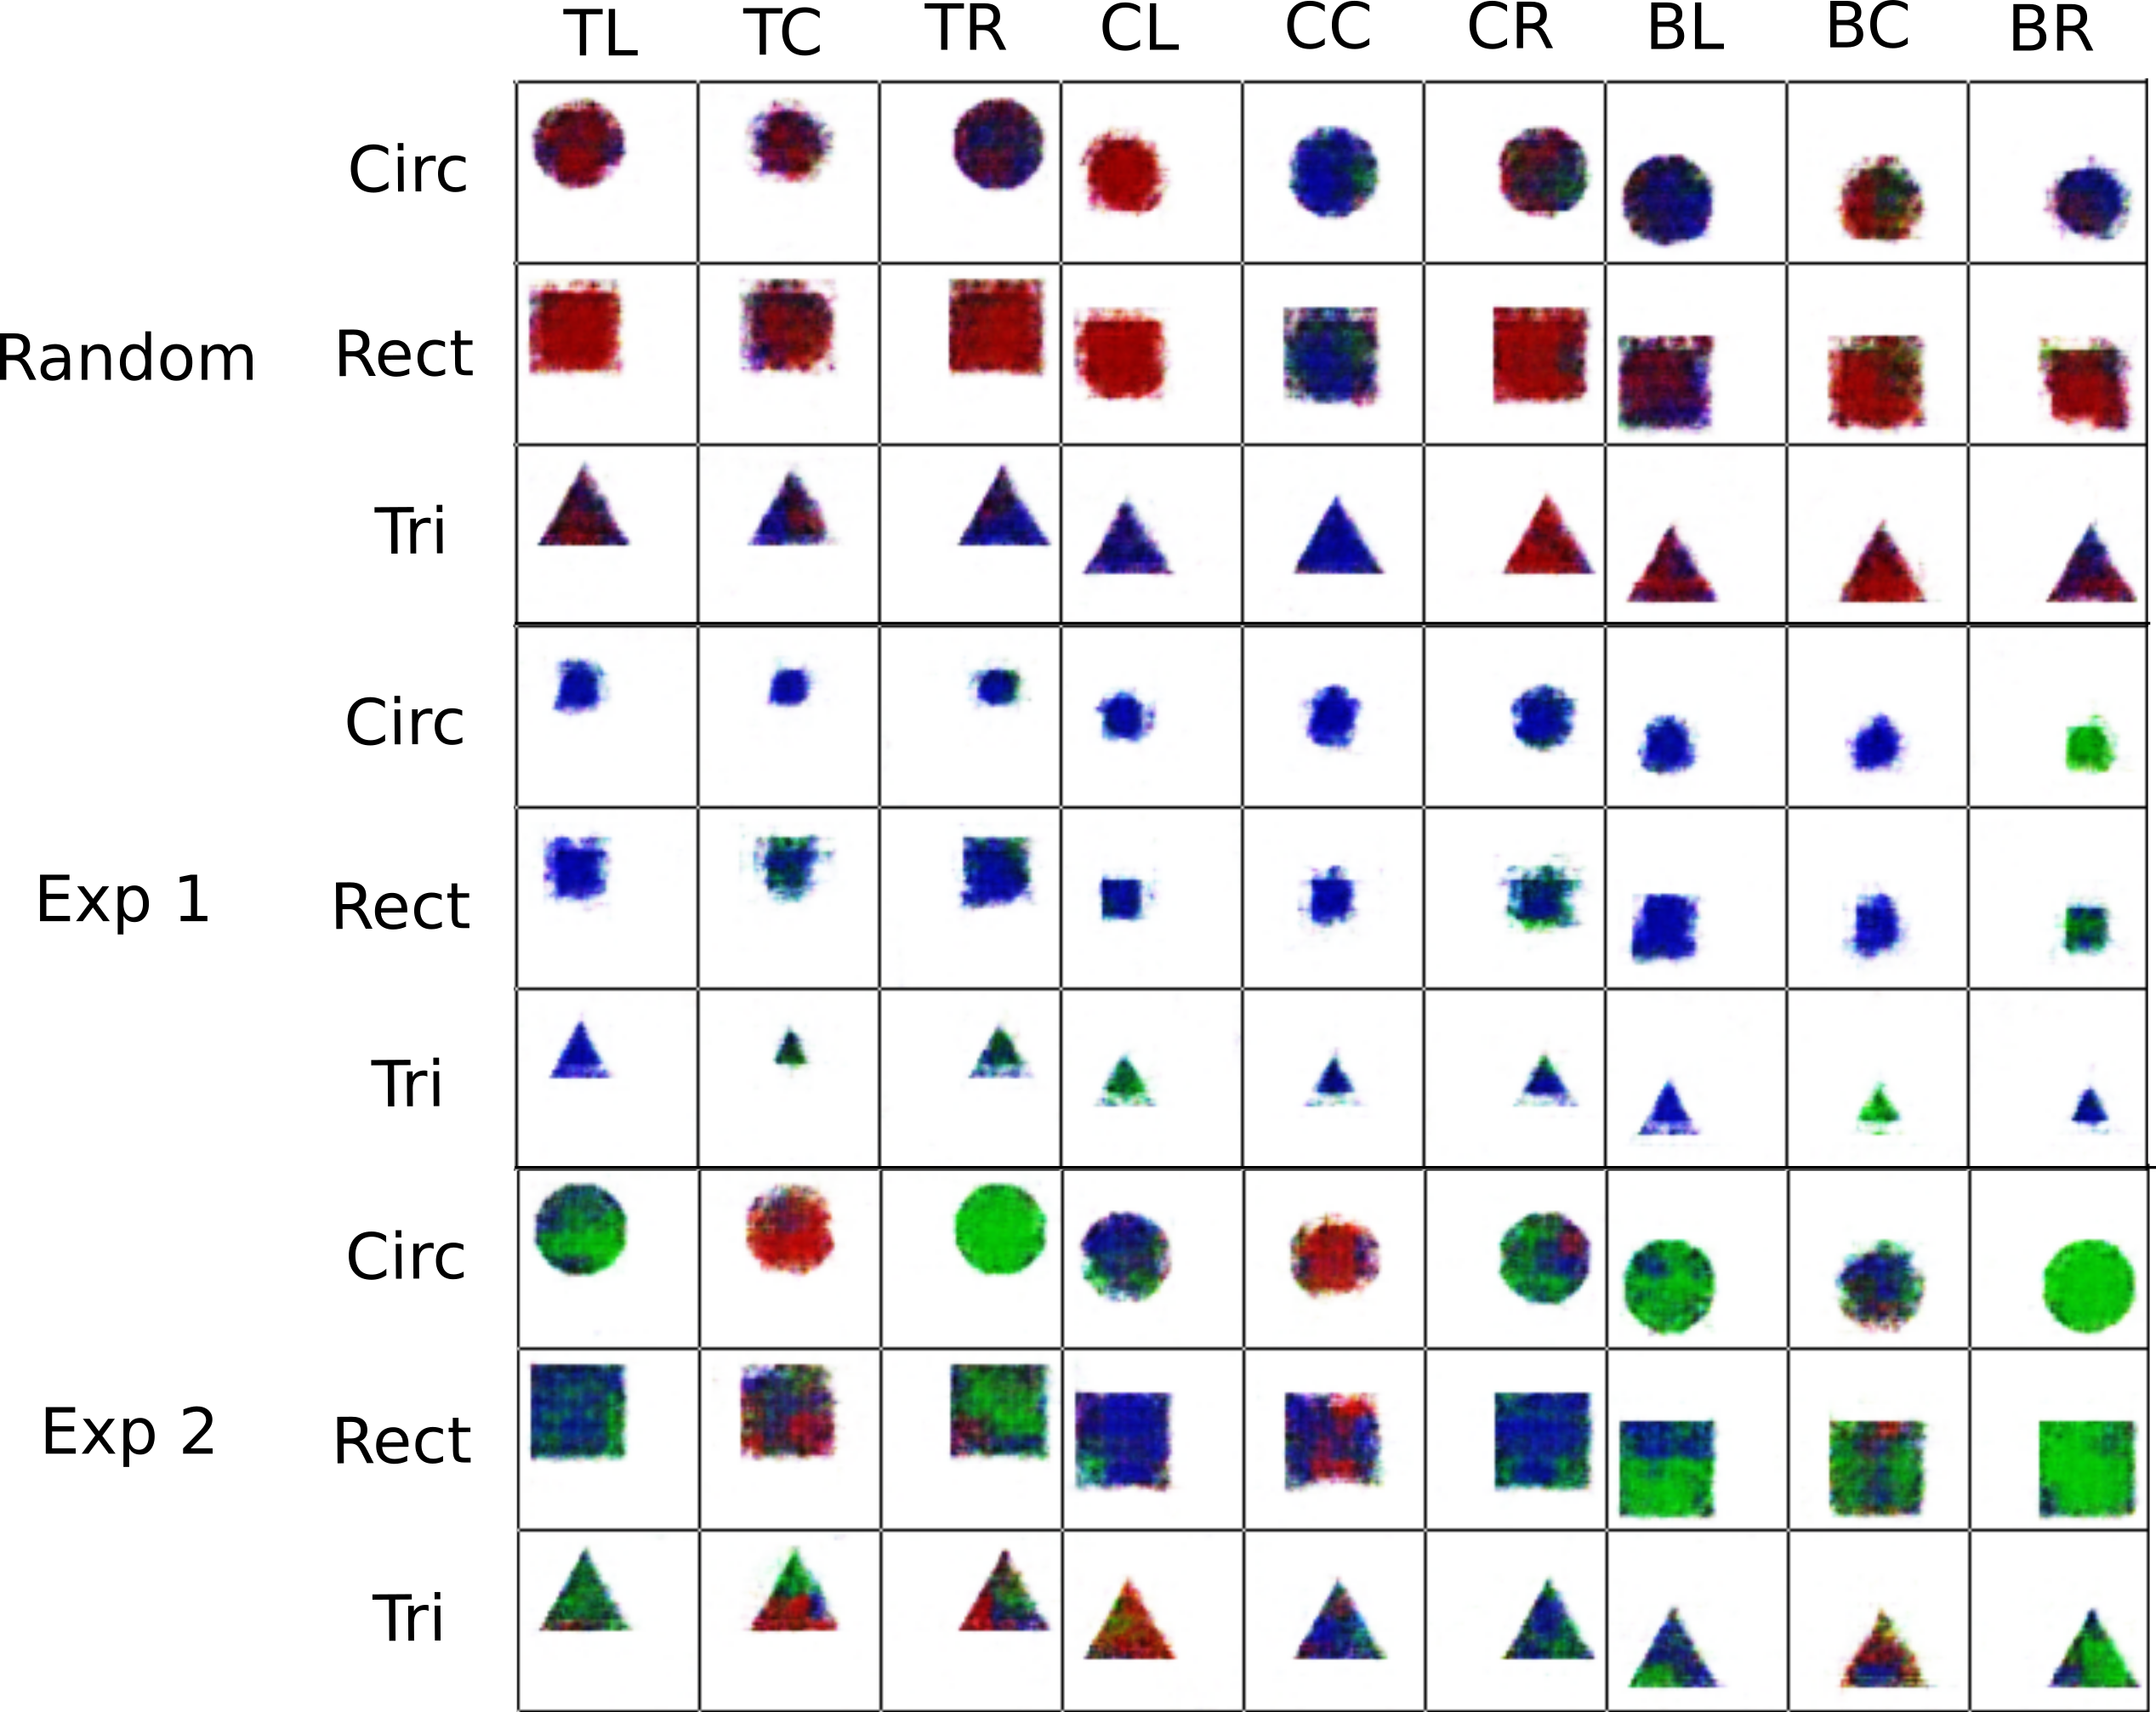
\includegraphics[width=0.75\textwidth]{Figs/shapes/2word339_pos.png}
\caption{Experiment 3, run A: Images generated using word pairs.}
\label{fig:2word339}
\end{figure}

Initialising with weights from experiment 2 offers a marginal benifit, with each of the shapes being generally more solid in appearance. Full results from all four runs can be found in the supplimental materials.

\paragraph{Description Accuracy}

\begin{table}[h!]
\centering
	\begin{tabular}{|c|c|c|c|}
	\hline
	Initialisation & 	Bimodal & 	Image Only 	& 	Words Only \\ \hline
	Random	&	100.00	$\mypm$	0.00	&	98.51	$\mypm$	4.52	&	100.00	$\mypm$	0.00	\\ \hline
	Exp 1	&	100.00	$\mypm$	0.00	&	99.85	$\mypm$	0.50	&	100.00	$\mypm$	0.00	\\ \hline
	Exp 2	&	100.00	$\mypm$	0.00	&	\textbf{99.99}	$\mypm$ 0.03	&	100.00	$\mypm$	0.00	\\ \hline



	\end{tabular}
\caption{Experiment 3: Percentage Description Accuracy for different weight initialisations. }
\label{tab:res339_acc}
\end{table}

There is a clear effect on the accuracy of descriptions generated by the MAE when transfer learning is used. This is seen as the improved performance when generating descriptions in the Image Only testing condition as seen in \autoref{tab:res339_acc}.


\subsubsection{Discussion}
Though the addition of extra positions had a detrimental effect on the generation of images from single words, (see \autoref{fig:339single} and \autoref{fig:339single_pos}) the MAE was still able to correctly learn to ground all of the words of the descriptions. This becomes particularly apparent when pairs of words are provided as input, as in \autoref{fig:2word339}.

Taking an incremental approach to training by pretraining on a simpler task does not have a univerasally positive effect on the grounding of words to visual attributes. Whilst the weights from experiment 2 provided a small but noticable benifit when generating images from pairs of words over the random initialisation baseline, the weights from experiment 1 did not. 

\begin{table}
\centering
\begin{tabular}{|c|c|}
\hline
Initialisation & Total Weight Updates\\ \hline
Random &  1,215,000\\ \hline
Exp 1 &  540,000\\ \hline
Exp 2 &  810,000\\ \hline

\end{tabular}
\caption{Experiment 3: Total number of weight updates.}
\label{tab:updatesTotal}
\end{table}

Despite the MAE initialised with Random weights receiveing more total updates to its weights as seen in \autoref{tab:updatesTotal}, its performance is worse than both the MAE pretrained on experiment 1 and the MAE pretrained on experiment 2 in terms of both error and accuarcy. See \autoref{appendix:B} for an explanation of how the number of weight updates is calculated.

Having the MAE master the simpler tasks of either experiment 1 or 2 through pretraining, had a positive effect on both image and description generation in the Image Only testing condition. This also carried over to the accuracy of description generation in this condition. This shows that by first learning to ground a smaller number of visual attributes to the words that describe them, the MAE is better able to correctly learn the additional words of the new datasubset (improved description accuracy) and be more confident about the meaning of these visual attributes (lower MSE).


\newpage
\subsection{Experiment 4}
For this experiment we will make use of all of the data in ArtS as shown in \autoref{tab:Arts_desc}. Again I will explore the affects of incremental learning, utilising the prelearned weights of experiments 1 and 2 and 3. This will allow me to examine whether having a larger number of concepts (words and their image equivalents) mastered  helps learning new concepts or whether one can simply learn all concepts simultaneously.

The different initialisation schemes will be referred to as: Random: randomly initialised weights, Exp1: the weights trained during experiment 1, Exp2: the weights trained during experiment 2, Exp 3: the weights trained during experiment 3 starting from random initialisation.
%, Exp 1+3: the weights trained during experiment 3 starting with the weights from experiment 1, Exp 2+3: the weights trained during experiment 3 starting with the weights from experiment 2.
%Two other conditions, Random 80 and Random 100 utilise a random initialisations but have 80 and 100 samples per object respectively compared to the 50 samples per object used in all other conditions.
%

\subsubsection{Results}

\begin{table}[h!]
\centering
	\begin{tabular}{|c|c|c|c|}
	\hline
	Initialisation & 	Bimodal & 	Image Only 	& 	Words Only \\ \hline
Random 	&	3.82	$\mypm$	0.30	&	54.12	$\mypm$	43.74	&	3.96	$\mypm$	0.22	\\ \hline
Exp 1	&	\textbf{3.73}	$\mypm$	0.06	&	9.33	$\mypm$	9.71	&	\textbf{3.91}	$\mypm$	0.04\\ \hline
Exp 2	&	3.80	$\mypm$	0.19	&	\textbf{8.55}	$\mypm$	4.70	&	3.96	$\mypm$	0.20	\\ \hline
Exp 3	&	3.75	$\mypm$	0.02	&	14.28	$\mypm$	12.18	&	3.93	$\mypm$	0.05	\\ \hline
%Exp1+3	&	3.77	$\mypm$	0.14	&	16.17	$\mypm$	17.96	&	3.97	$\mypm$	0.13	\\ \hline
%Exp 2+3	&	3.76	$\mypm$	0.12	&	33.08	$\mypm$	57.02	&	3.92	$\mypm$	0.06	\\ \hline

	\end{tabular}
\caption{Experiment 4: Total MSE for different weight initialisations. (All values are $\times10^{-3}$)}
\label{tab:res739}
\end{table}

The results for each method of initialising the weights of the MAE in experiment 4 can be seen in \autoref{tab:res739}. Whilst in the Bimodal and Word Only testing conditions, initialising with random weights gave the best loss, this is not the case in the Words Only testing condition where the random weight initialisation performs an order of magnitude worse than any of the other initialisation schemes.


\paragraph{Image Generation}

Once again we see a clear distinction between the three sizes as shown in \autoref{fig:739single_shape}, this is independent of starting condition. However, whilst there are clear distinctions between the three shapes for all starting conditions, with the exception of initialising with weights from experiment 2 it is not clear that the shapes have been correctly learnt.

\begin{figure}[h]
\centering
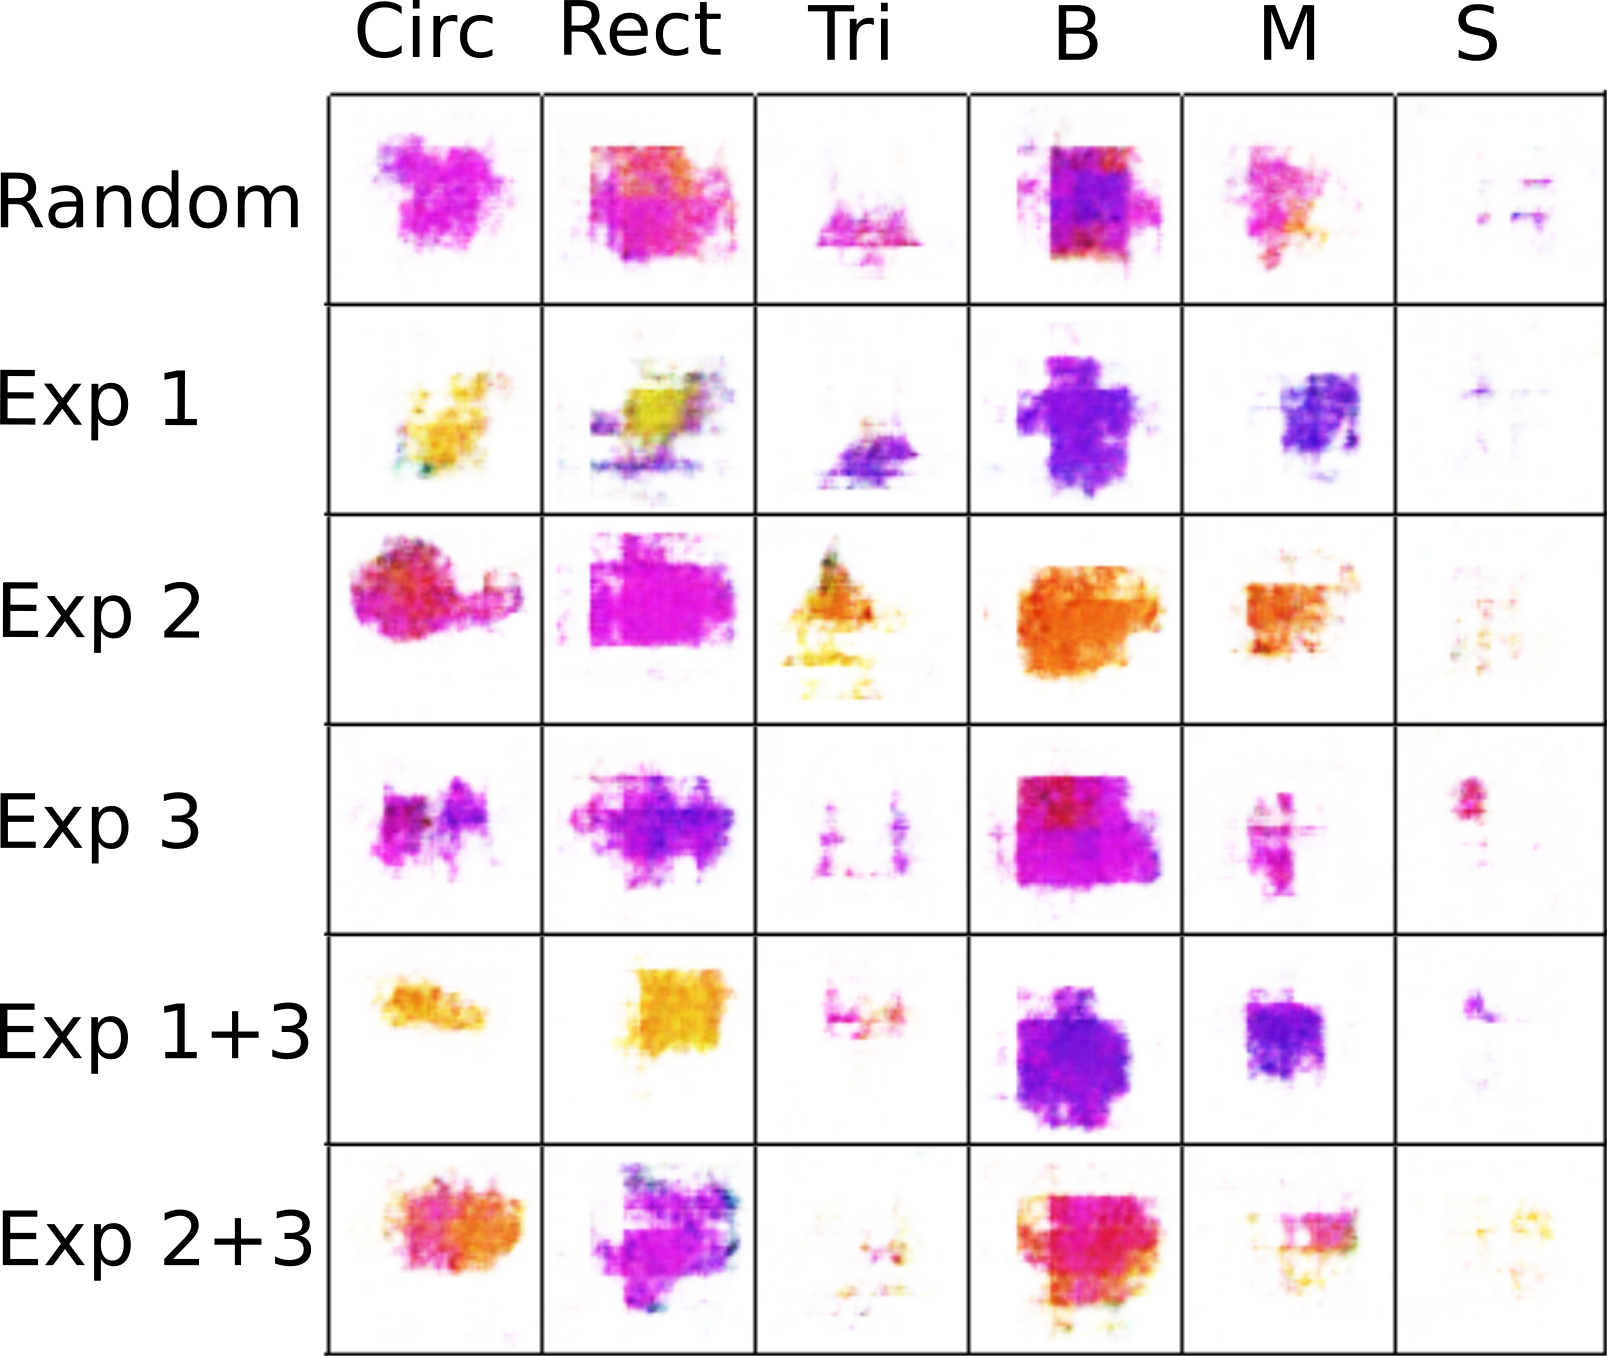
\includegraphics[width=0.75\textwidth]{Figs/shapes/singlelabel739_shape.png}
\caption{Experiment 4, run A: Images generated from shape, colour and size words for different weight initialisation conditions.}
\label{fig:739single_shape}
\end{figure}



\begin{figure}[h!]
\centering
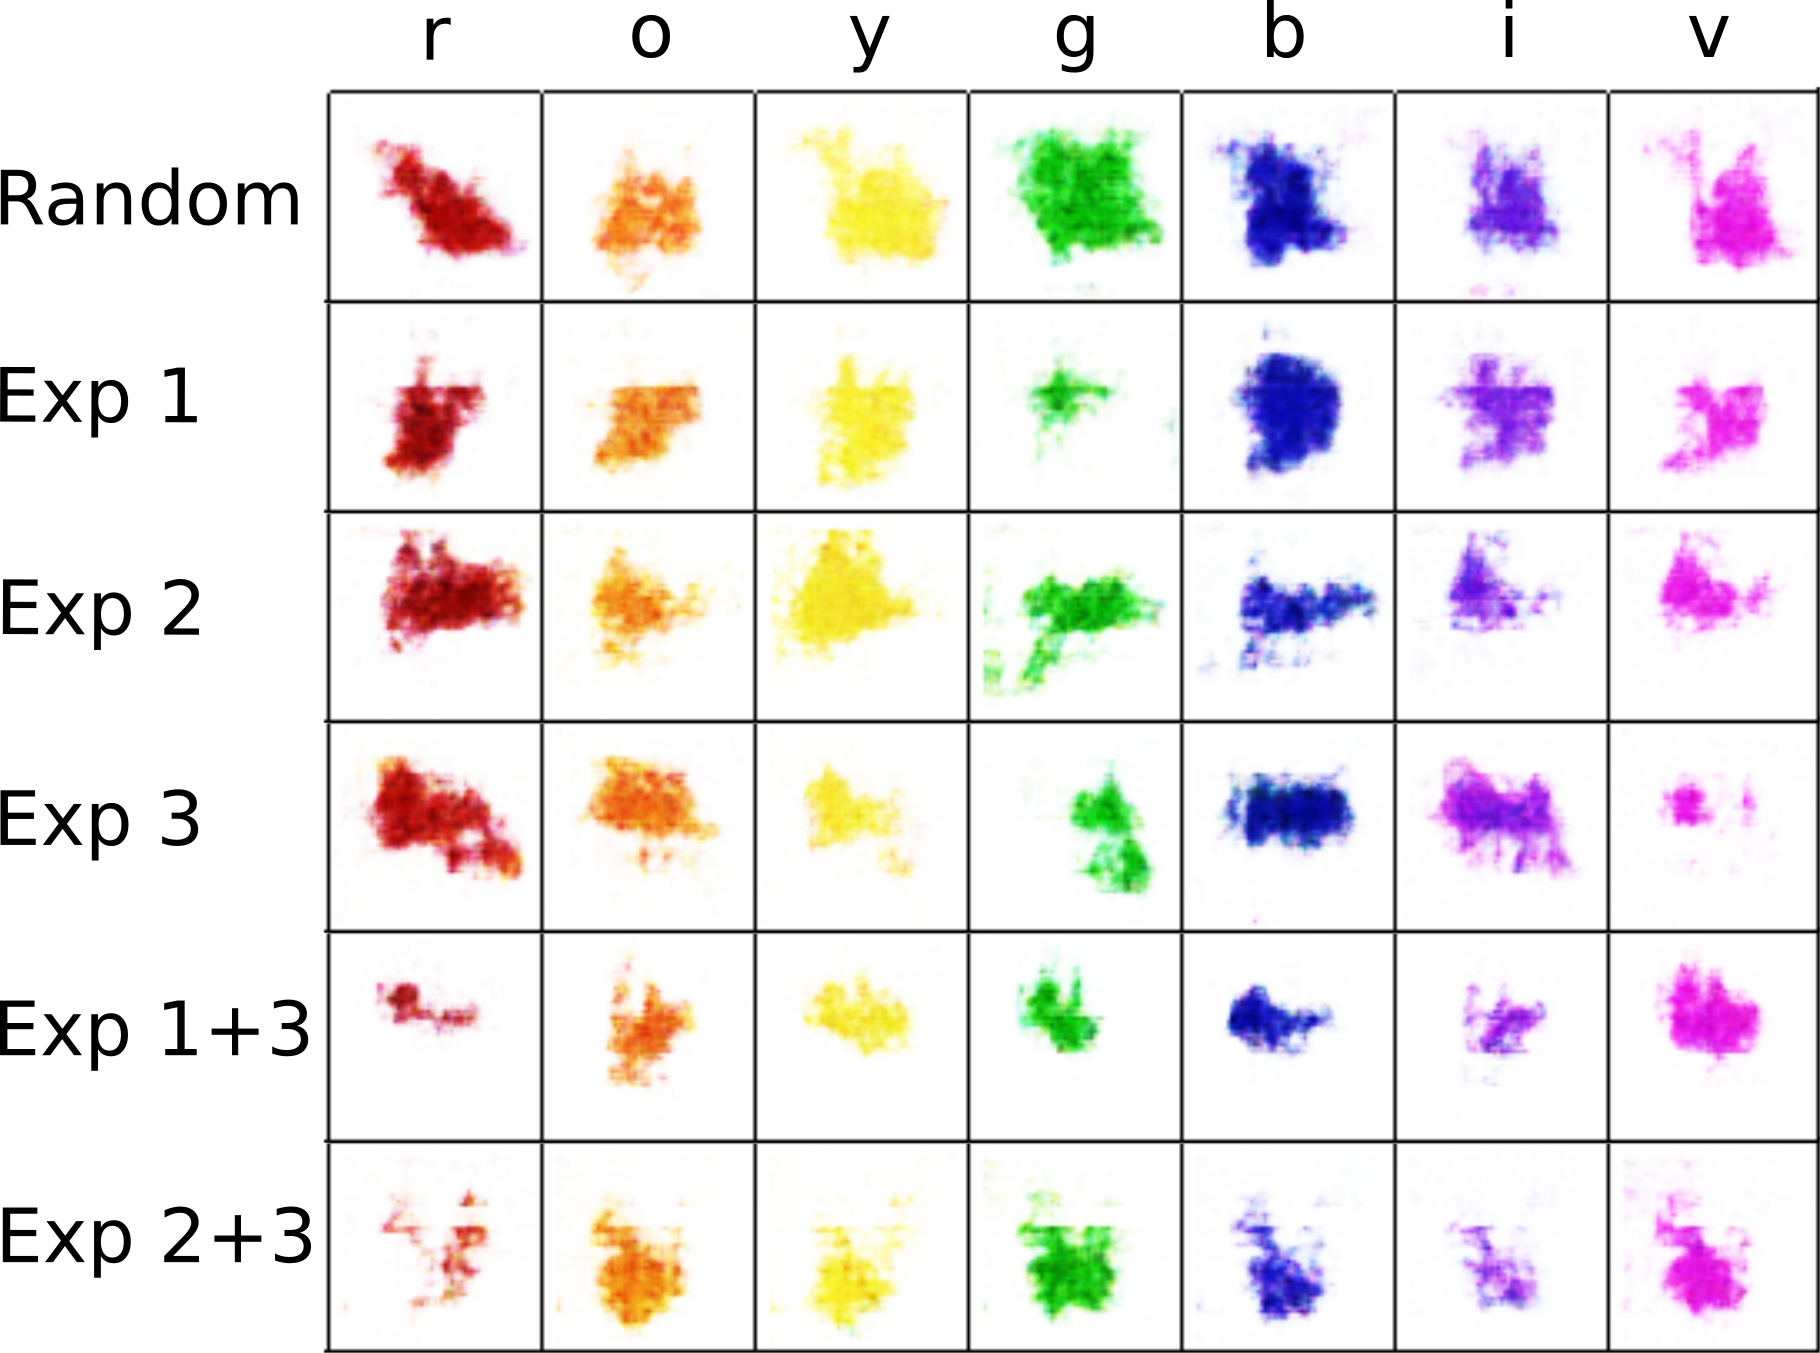
\includegraphics[width=0.75\textwidth]{Figs/shapes/singlelabel739_col.png}
\caption{Experiment 4, run A: Images generated from each colour word for different weight initialisation conditions.}
\label{fig:739single_col}
\end{figure}

\begin{figure}[h]
\centering
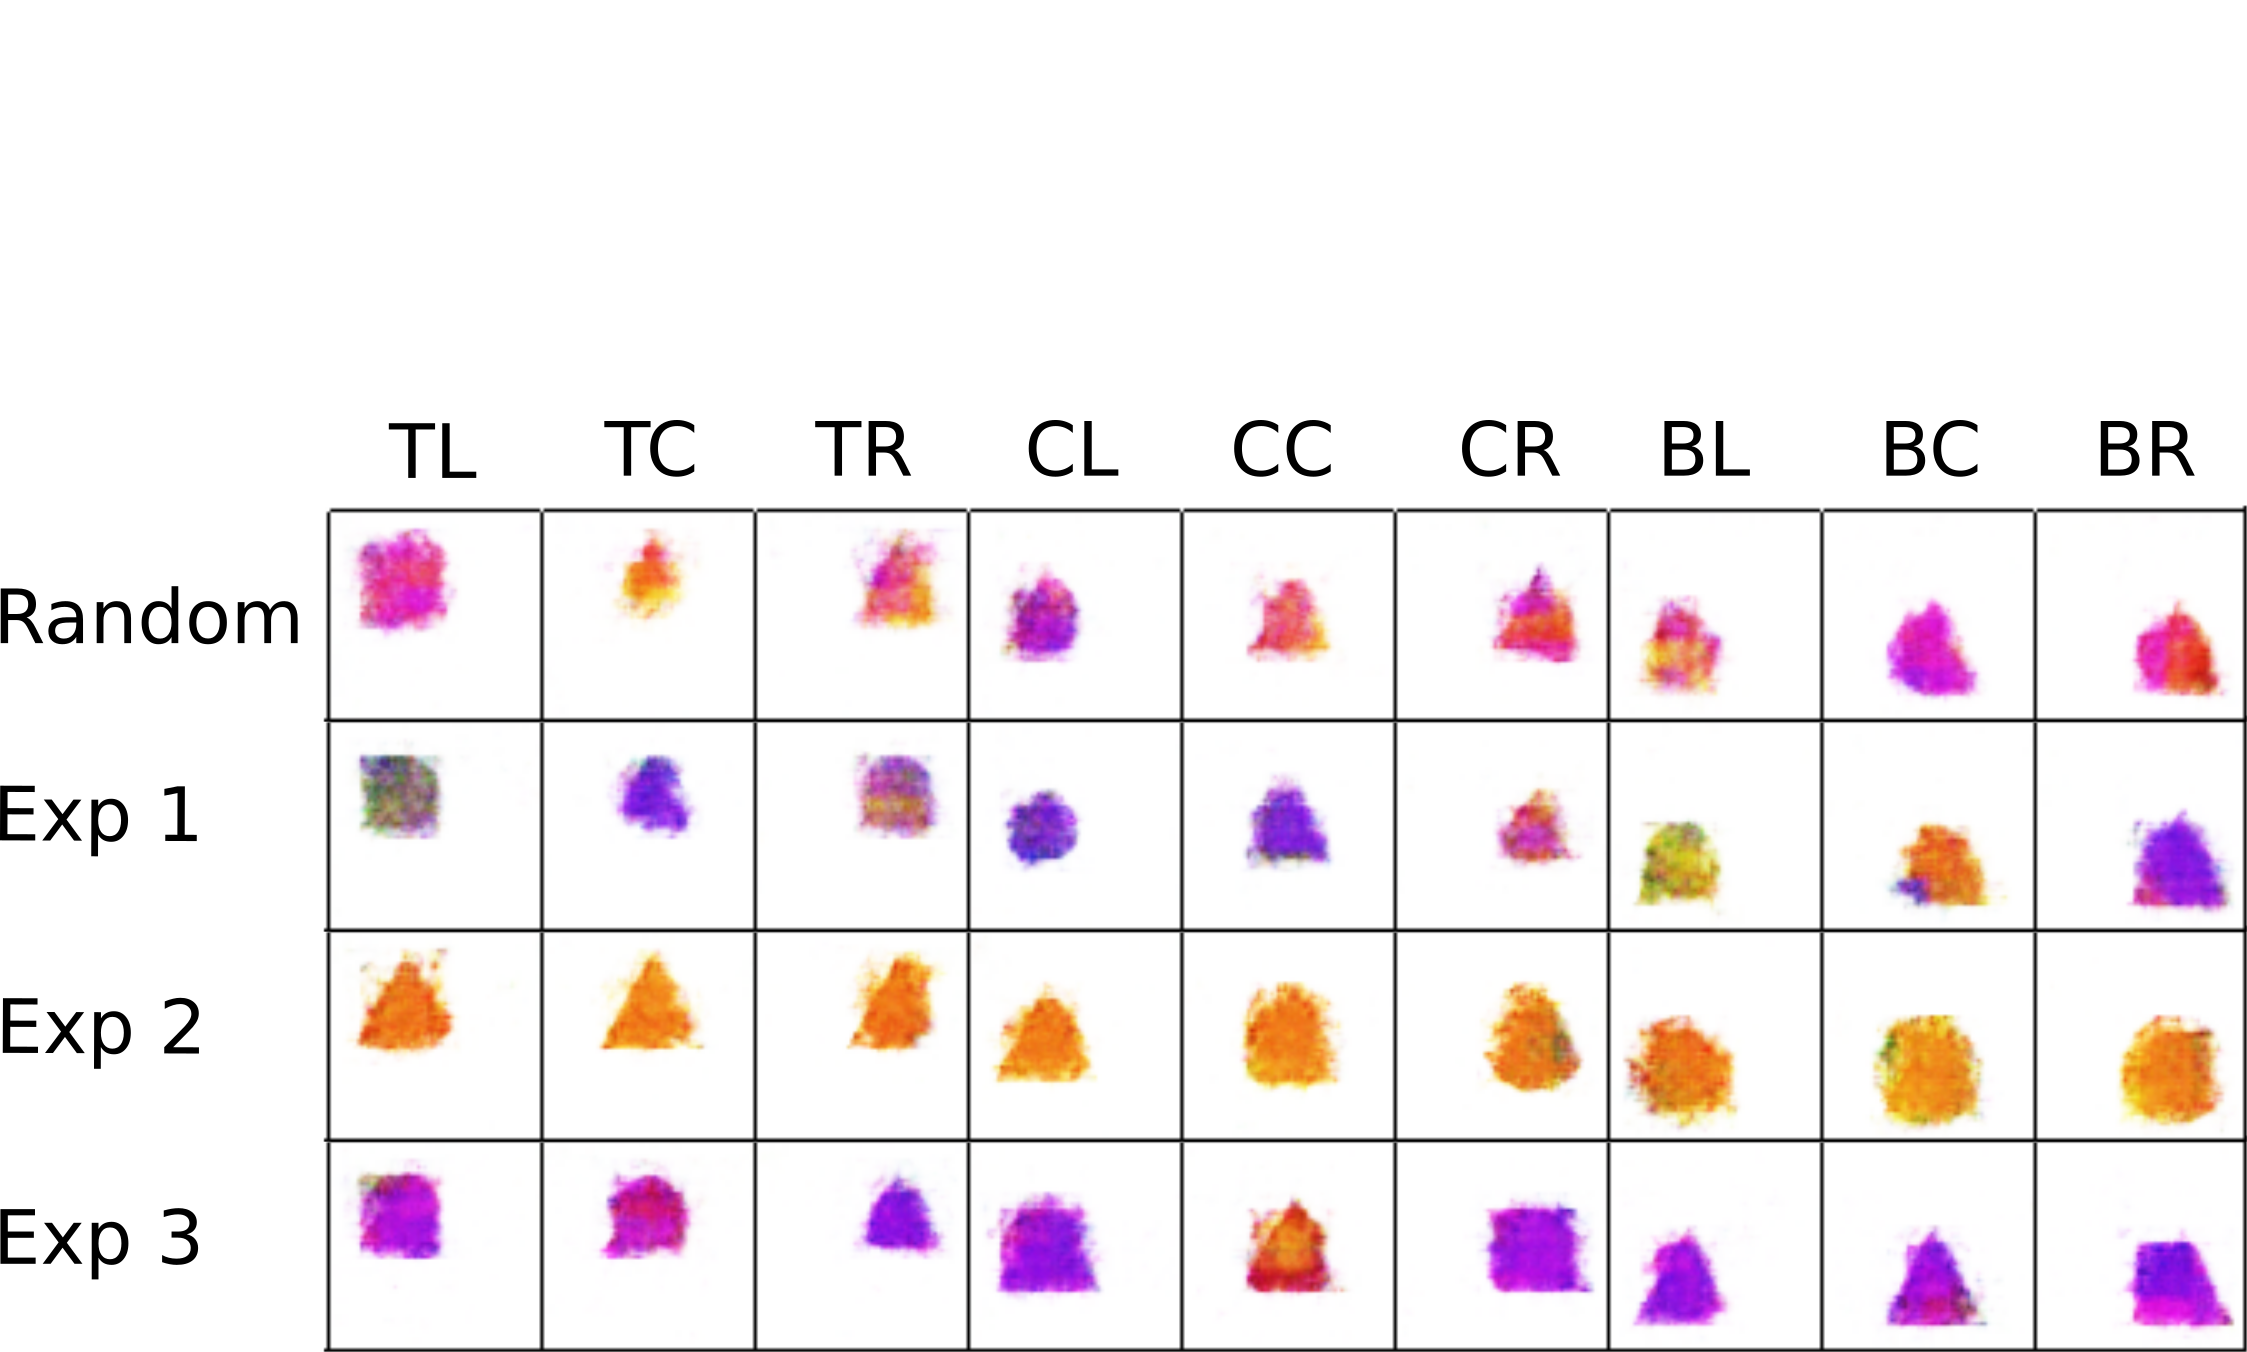
\includegraphics[width=0.75\textwidth]{Figs/shapes/singlelabel739_pos.png}
\caption{Experiment 4, run A: Images generated from each position word for different weight initialisation conditions.}
\label{fig:739single_pos}
\end{figure}

All seven colours are correctly learnt as seen in \autoref{fig:739single_col} for all weight initialisation conditions. As are all 9 positions as seen in \autoref{fig:739single_pos}




\begin{figure}[h!]
\centering
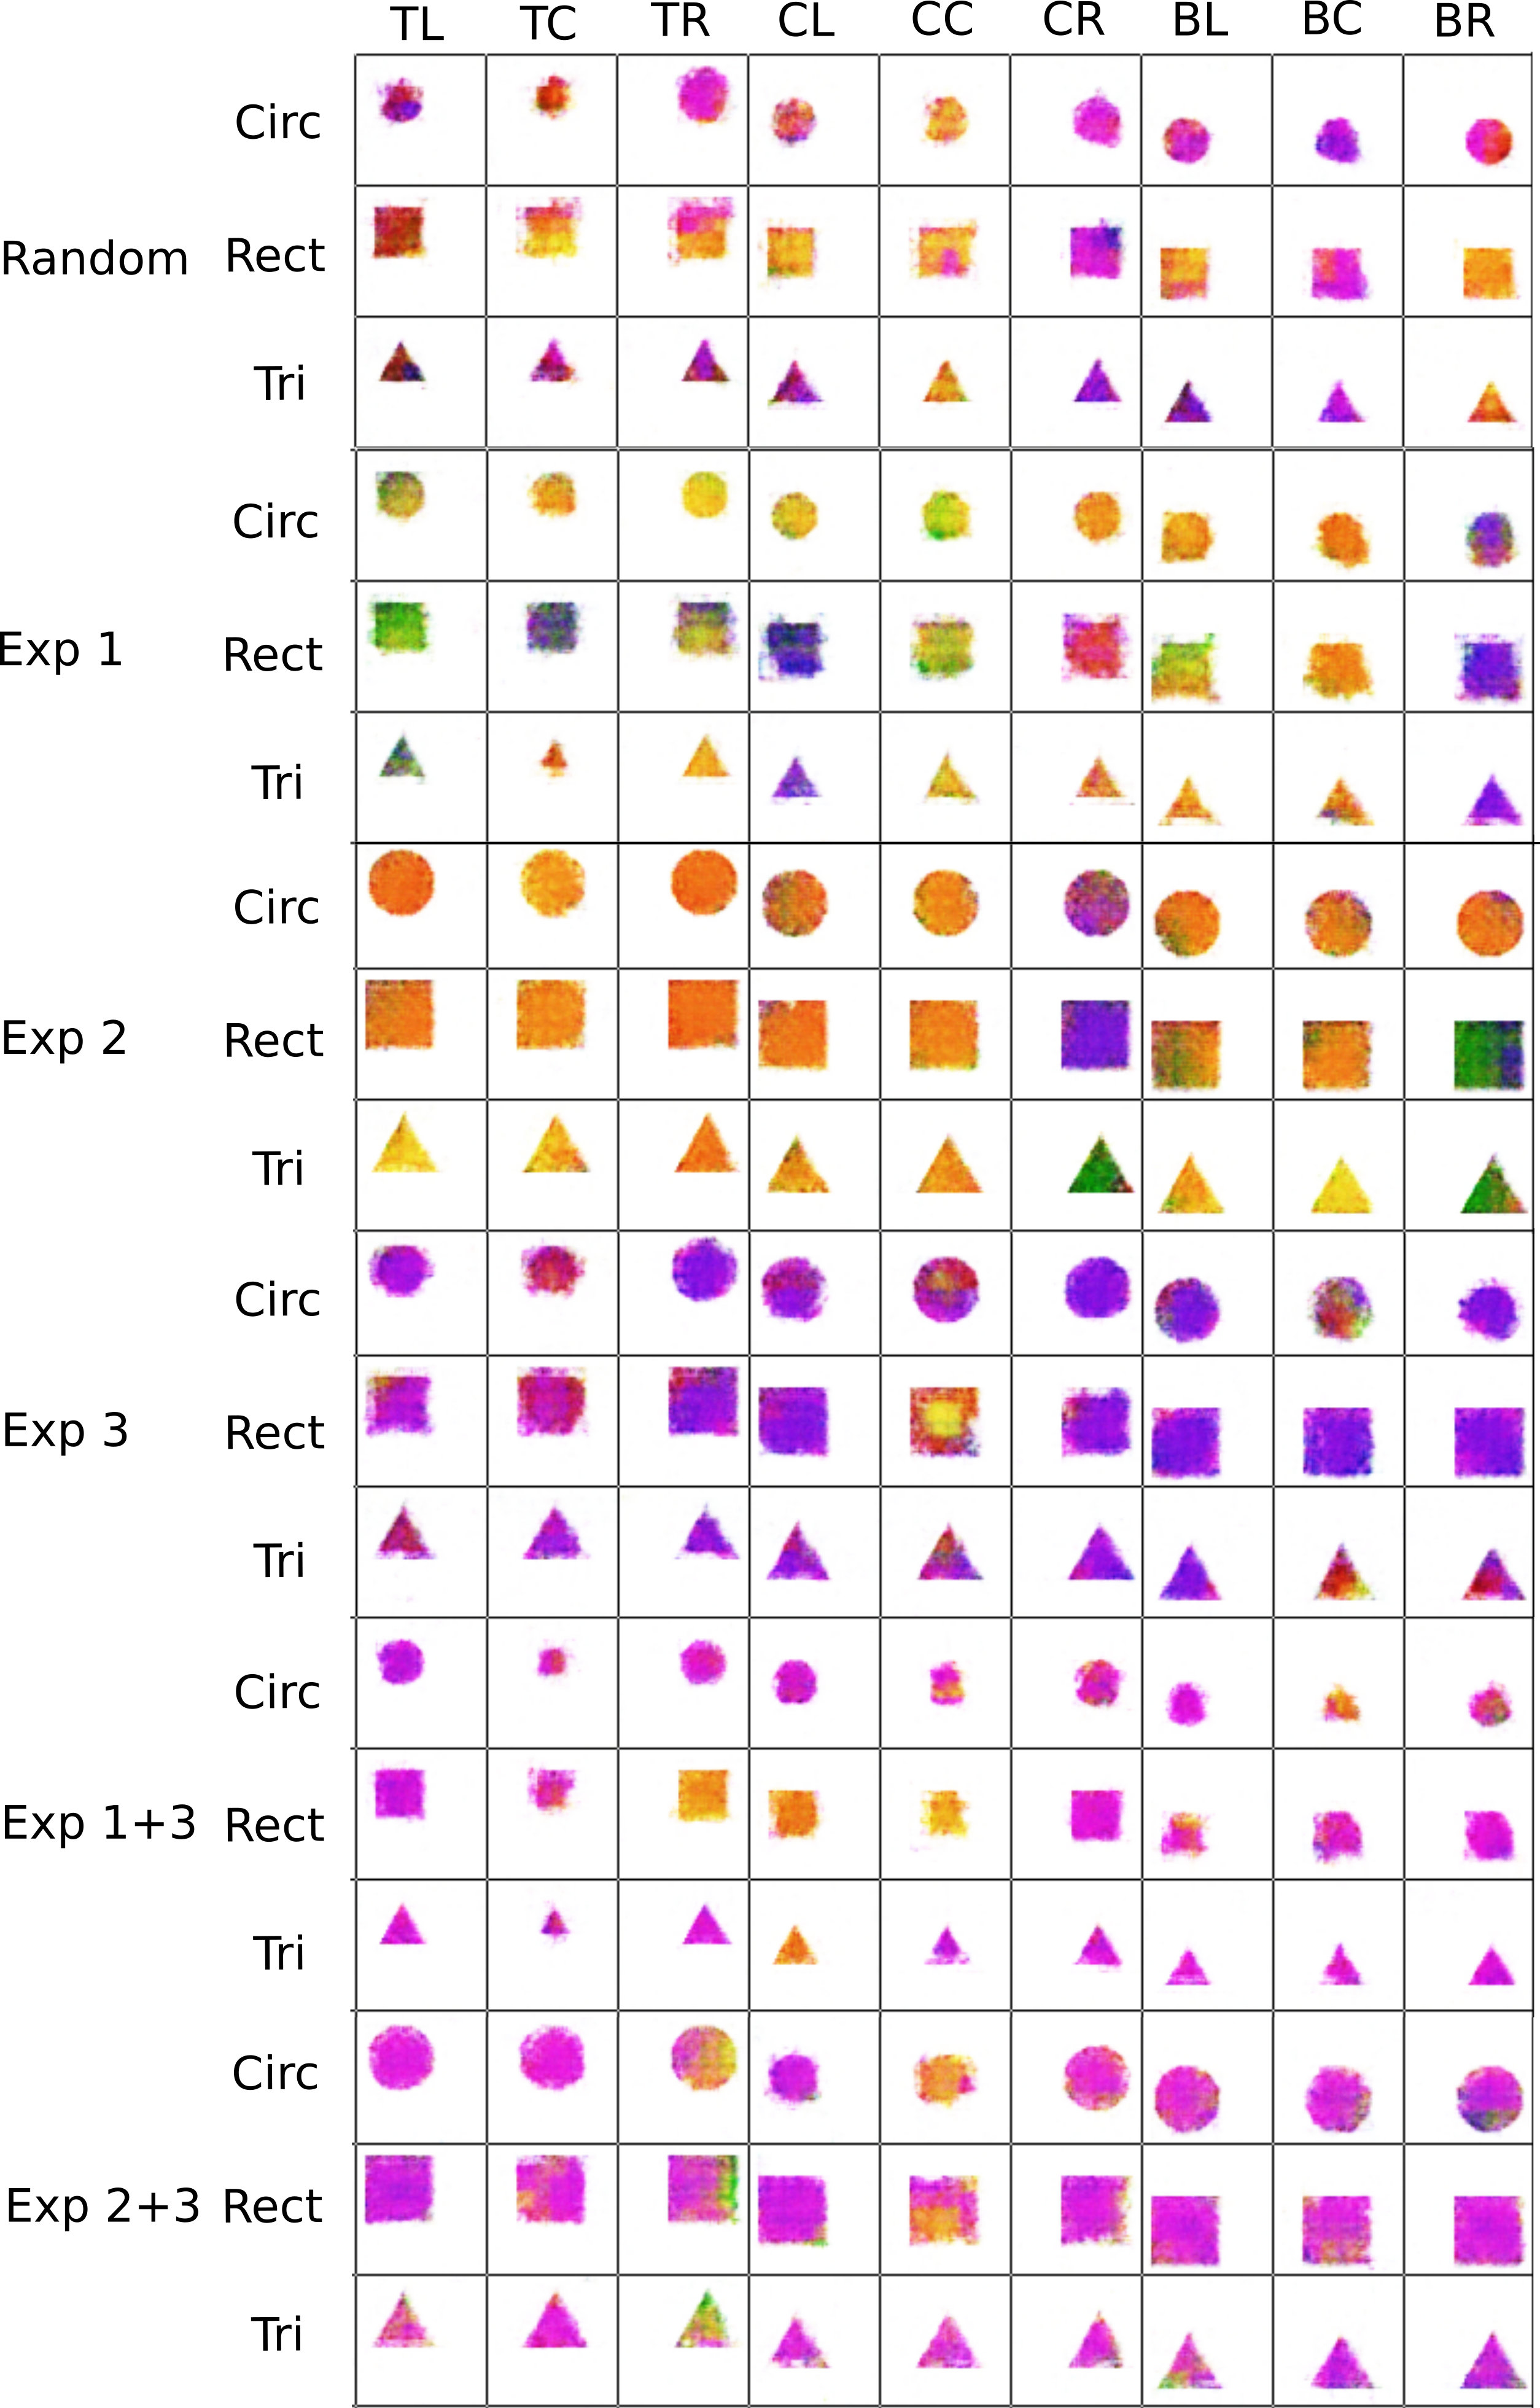
\includegraphics[width=0.75\textwidth]{Figs/shapes/2word739_pos.png}
\caption{Experiment 4, run A: Images generated using word pairs.}
\label{fig:2word739}
\end{figure}

The addition of pretraining has a positive effect on the grounding of the meaning of all words, however this is particularly clear in the case of the shape words, \textsc{Circle}, \textsc{Rectangle} and\textsc{Triangle}. \autoref{fig:2word739} shows that without pretraining, the shapes generated by the MAE when two words are given as input (a shape and position), are somewhat fuzzy and incorrect. For example, generating an image from the words \textsc{Circle, Centre Right} leads to a \textit{Circle} with protrusions in the random initialisation condition.

Pretraining on experiment 2 gave the best results, with all shapes apearing solid and correctly positioned without extraneous edges or protrusions. 

Comparing \autoref{fig:2word739} to the errors in \autoref{tab:res739}, we would expect the best image generation to occur when using the MAE initalised with random weights, however, this suggests that the MAE has learnt the meaning of the descriptions as a whole and has not grounded the meanings of the individual words which make up the descriptions.

\paragraph{Description Accuracy}


\begin{table}[h!]
\centering
	\begin{tabular}{|c|c|c|c|}
	\hline
	Initialisation & 	Bimodal & 	Image Only 	& 	Words Only \\ \hline
Random 	&	100.00	$\mypm$	0.00	&	96.10	$\mypm$	6.29	&	100.00	$\mypm$	0.00	\\ \hline
Exp 1	&	100.00	$\mypm$	0.00	&	99.49	$\mypm$	2.21	&	100.00	$\mypm$	0.00	\\ \hline
Exp 2	&	100.00	$\mypm$	0.00	&	\textbf{99.53}	$\mypm$	1.22	&	100.00	$\mypm$	0.00\\ \hline
Exp 3	&	100.00	$\mypm$	0.00	&	99.06	$\mypm$	2.42	&	100.00	$\mypm$	0.00\\ \hline
%Exp 1+3	&	100.00	$\mypm$	0.00	&	98.81	$\mypm$	2.69	&	100.00	$\mypm$	0.00\\ \hline
%Exp 2+3	&	100.00	$\mypm$	0.00	&	97.63	$\mypm$	6.54	&	100.00	$\mypm$	0.00\\ \hline

	\end{tabular}
\caption{Experiment 4: Percentage Description Accuracy for different weight initialisations.}
\label{tab:res739acc}
\end{table}

The addition of more variety of colours to the dataset has had a negative effect on description accuracy in the Image Only testing condition, with a small number of images being mislabelled. The MAE initialised with weights from expeirment 2 performed the best with a description generation accuracy of 99.53\% (compared to 99.99\% for the top performing model in experiment 3).

Unsurprisingly, the MAE initialised with weights from experiment 2 has the best description accuracy in the image only testing condition. Given that this MAE also produces the best images from individual and pairs of words, it is clear that bidirectional grounding has occured in this condition. The MAE is able to generate the correct visual attributes from the input words and is also able to correctly describe the visual attributes of images.

\subsubsection{Discussion}
As in experiment 3 there is a clear positive effect of utilising an incremental approach to grounding the meanings of the words and the visual attributes they equate to. 
When training from random weights, the MAE struggles to generate images and descriptions in the Image Only test condition, with a four-fold cross-validated MSE that is an order of magnitude worse than the best performing pretrained models.

\begin{table}
\centering
\begin{tabular}{|c|c|}
\hline
Initialisation & Total Weight Updates\\ \hline
Random (50 Epochs) &  1,417,500\\ \hline
Random (100 Epochs) & 2,835,000\\ \hline
Exp 1 & 1,485,000\\ \hline
Exp 2 & 1,620,000\\ \hline
Exp 3 &	2,025,000\\ \hline

\end{tabular}
\caption{Experiment 4: Total number of weight updates.}
\label{tab:updatesTotal4}
\end{table}

Again, the best performing MAE didn't recieve the most training updates. However, the worse performance of the MAE initialised with random weights is not only due to overfitting from making too many updates to its weights. Even after 50 epochs of training, the randomly initalised MAE had poor performance despite only updating its weights 1.4 million times, compared to the 1.6 million updates of the MAE initialised with weights from experiment 2. The better performance after 50 epochs  of training compared to after 100 epochs of training suggests that some overfitting has occured (\autoref{tab:res739_50}).

\begin{table}[h!]
\centering
\begin{tabular}{|c|c|c|c|}
	\hline
	Measure & 	Bimodal & 	Image Only 	& 	Words Only \\ \hline
MSE	&	3.82	$\mypm$	0.12	&	32.58	$\mypm$	36.49	&	4.00	$\mypm$	0.10	\\ \hline
Accuracy	&	100.00	$\mypm$	0.00	&	97.44	$\mypm$	5.77	&	100.00	$\mypm$	0.00\\ \hline
\end{tabular}

\caption{Experiment 4: Mean Squared Error ($\times10^{-3}$) and Percentage Description Accuracy for the randomly initialised MAE after 50 epochs of training.} 
\label{tab:res739_50}
\end{table}


In both experiments 3 and 4, the best performance was seen from the MAE initialised with weights from experiment 2 (Exp 2). It is not obvious why this is. The Exp 2 weights achieved good performance in all testing conditions in experiment 2 (\autoref{tab:res333}). Compare this to the Exp 3 weights, which performed poorly when tested in experiment 3 in the Image Only condition (\autoref{tab:res339}). This suggests that grounding of the visual attributes was not achieved and explains why the MAE from experiment 4 initialised with Exp 3 weights does not perform as well as the MAE initialised with Exp 2 weights. The Exp 2 had learnt to bidrectionally ground all of the words and visual attributes of experiment 2. The Exp 3 weights had not learnt to bidirectionally ground all of the words and visual attributes of experiment 3.

Whilst the weights Exp 1 performed well in experiment 1 (\autoref{tab:res331}, they did not perform as well as the Exp 2 weights in experiment 2 (\autoref{tab:res333}) suggesting the qualtiy of the grounding was slightly lower. Further to this, there is a much bigger difference between the types of objects seen by the Exp 1 weights and those seen in experiments 3 and 4, meaning that the MAE initialised with the Exp 1 weights has more to learn than the MAE initialised with Exp 2 weights.

So, the Exp 2 weights likely lead to the best performance due to 2 factors, 1) the types of objects used to train it are more similar to those used in experiments 3 and 4 compared to those seen by the Exp 1 weights and 2) they have achieved bidirectional grounding of data of experiment 2, as shown by their superior performance in experiment 2 compared to the Exp 3 weights which did not achieve bidirectional grounding of the data of experiment 3.


\subsection{Experiment 5}
In this experiment I select certain subsets of objects from the data to omit, such as violet circles or green triangles. Then demonstrate how images of these objects can still be generated from their descriptions or through vector arithematic, as well as how images of these objects can be correctly described by the network.

I will examine the omission of 3 different objects, these trials will be referred to as MAE 1: omission of green triangles'', MAE 2: omisssion of orange rectangles'' and MAE 3: omission of  violet circles''. Each MAE is initialised with random weights and trained for 50 epochs.

\subsubsection{Results}

When testing the MAEs with object types they have seen before (i.e. not objects which were ommited from the training data) the perfomance is similar to that of the randomly initilaised MAE of experiment 4. This is to be expected as the data and training setup is identical apart from the omitted objects (\autoref{tab:res_exp5}).
\begin{table}[h!]
\centering
	\begin{tabular}{|c|c|c|c|}
	\hline
Trial & 	Bimodal & 	Image Only 	& 	Words Only \\ \hline
MAE 1	&	3.87	$\mypm$	0.23	&	43.22	$\mypm$	44.88	&	4.05	$\mypm$	0.24	\\ \hline
MAE 1*	&	5.21	$\mypm$	0.78	&	86.71	$\mypm$	75.11	&	5.28	$\mypm$	0.55	\\ \hline
MAE 2	&	3.72	$\mypm$	0.21	&	15.60	$\mypm$	23.65	&	3.97	$\mypm$	0.29	\\ \hline
MAE 2*	&	4.95	$\mypm$	1.02	&	41.54	$\mypm$	23.46	&	7.18	$\mypm$	2.74	\\ \hline
MAE 3	&	4.01	$\mypm$	0.32	&	43.95	$\mypm$	79.53	&	4.12	$\mypm$	0.09	\\ \hline
MAE 3*	&	3.07	$\mypm$	0.77	&	86.16	$\mypm$	123.74	&	2.67	$\mypm$	0.24	\\ \hline
\end{tabular}
\caption{Experiment 5: Total MSE. Alternating rows show MSE for the datasubset without the omitted data and MSE for only the omitted data (marked with *). (All values are $\times10^{-3}$)}
\label{tab:res_exp5}
\end{table}
Testing with only the omitted object, we see an increase in MSE, particularly for the Image Only testing condition. This is to be expected as the MAE has never seen these objects before, and will therefore be biased towards generating outputs which are more simlar to its training data than those required to perform well at generating the correct output for the omitted objects (\autoref{tab:res_exp5}).

\paragraph{Image Generation}
To further demonstrate the abilities of multimodal representation learning through the use of a MAE, I used three subsets of data to train three MAEs. Each of the MAEs was trained 4 times for validation purposes as with all other experiments, the mean result for the four runs is presented.

For each training subset, a shape of a particular colour was omitted from the training data. In \autoref{fig:739_minus1}, MAEs 1, 2 and 3 were trained without green triangles, orange rectangles and violet circles, respectively. Generating images from full descriptions still results in correctly generating images of green triangles, orange rectangles and violet circles, showing that each MAE has learnt the meaning of these words individually and hence can ``imagine'' what their combinations should look like. 

\begin{figure}[h]
\centering
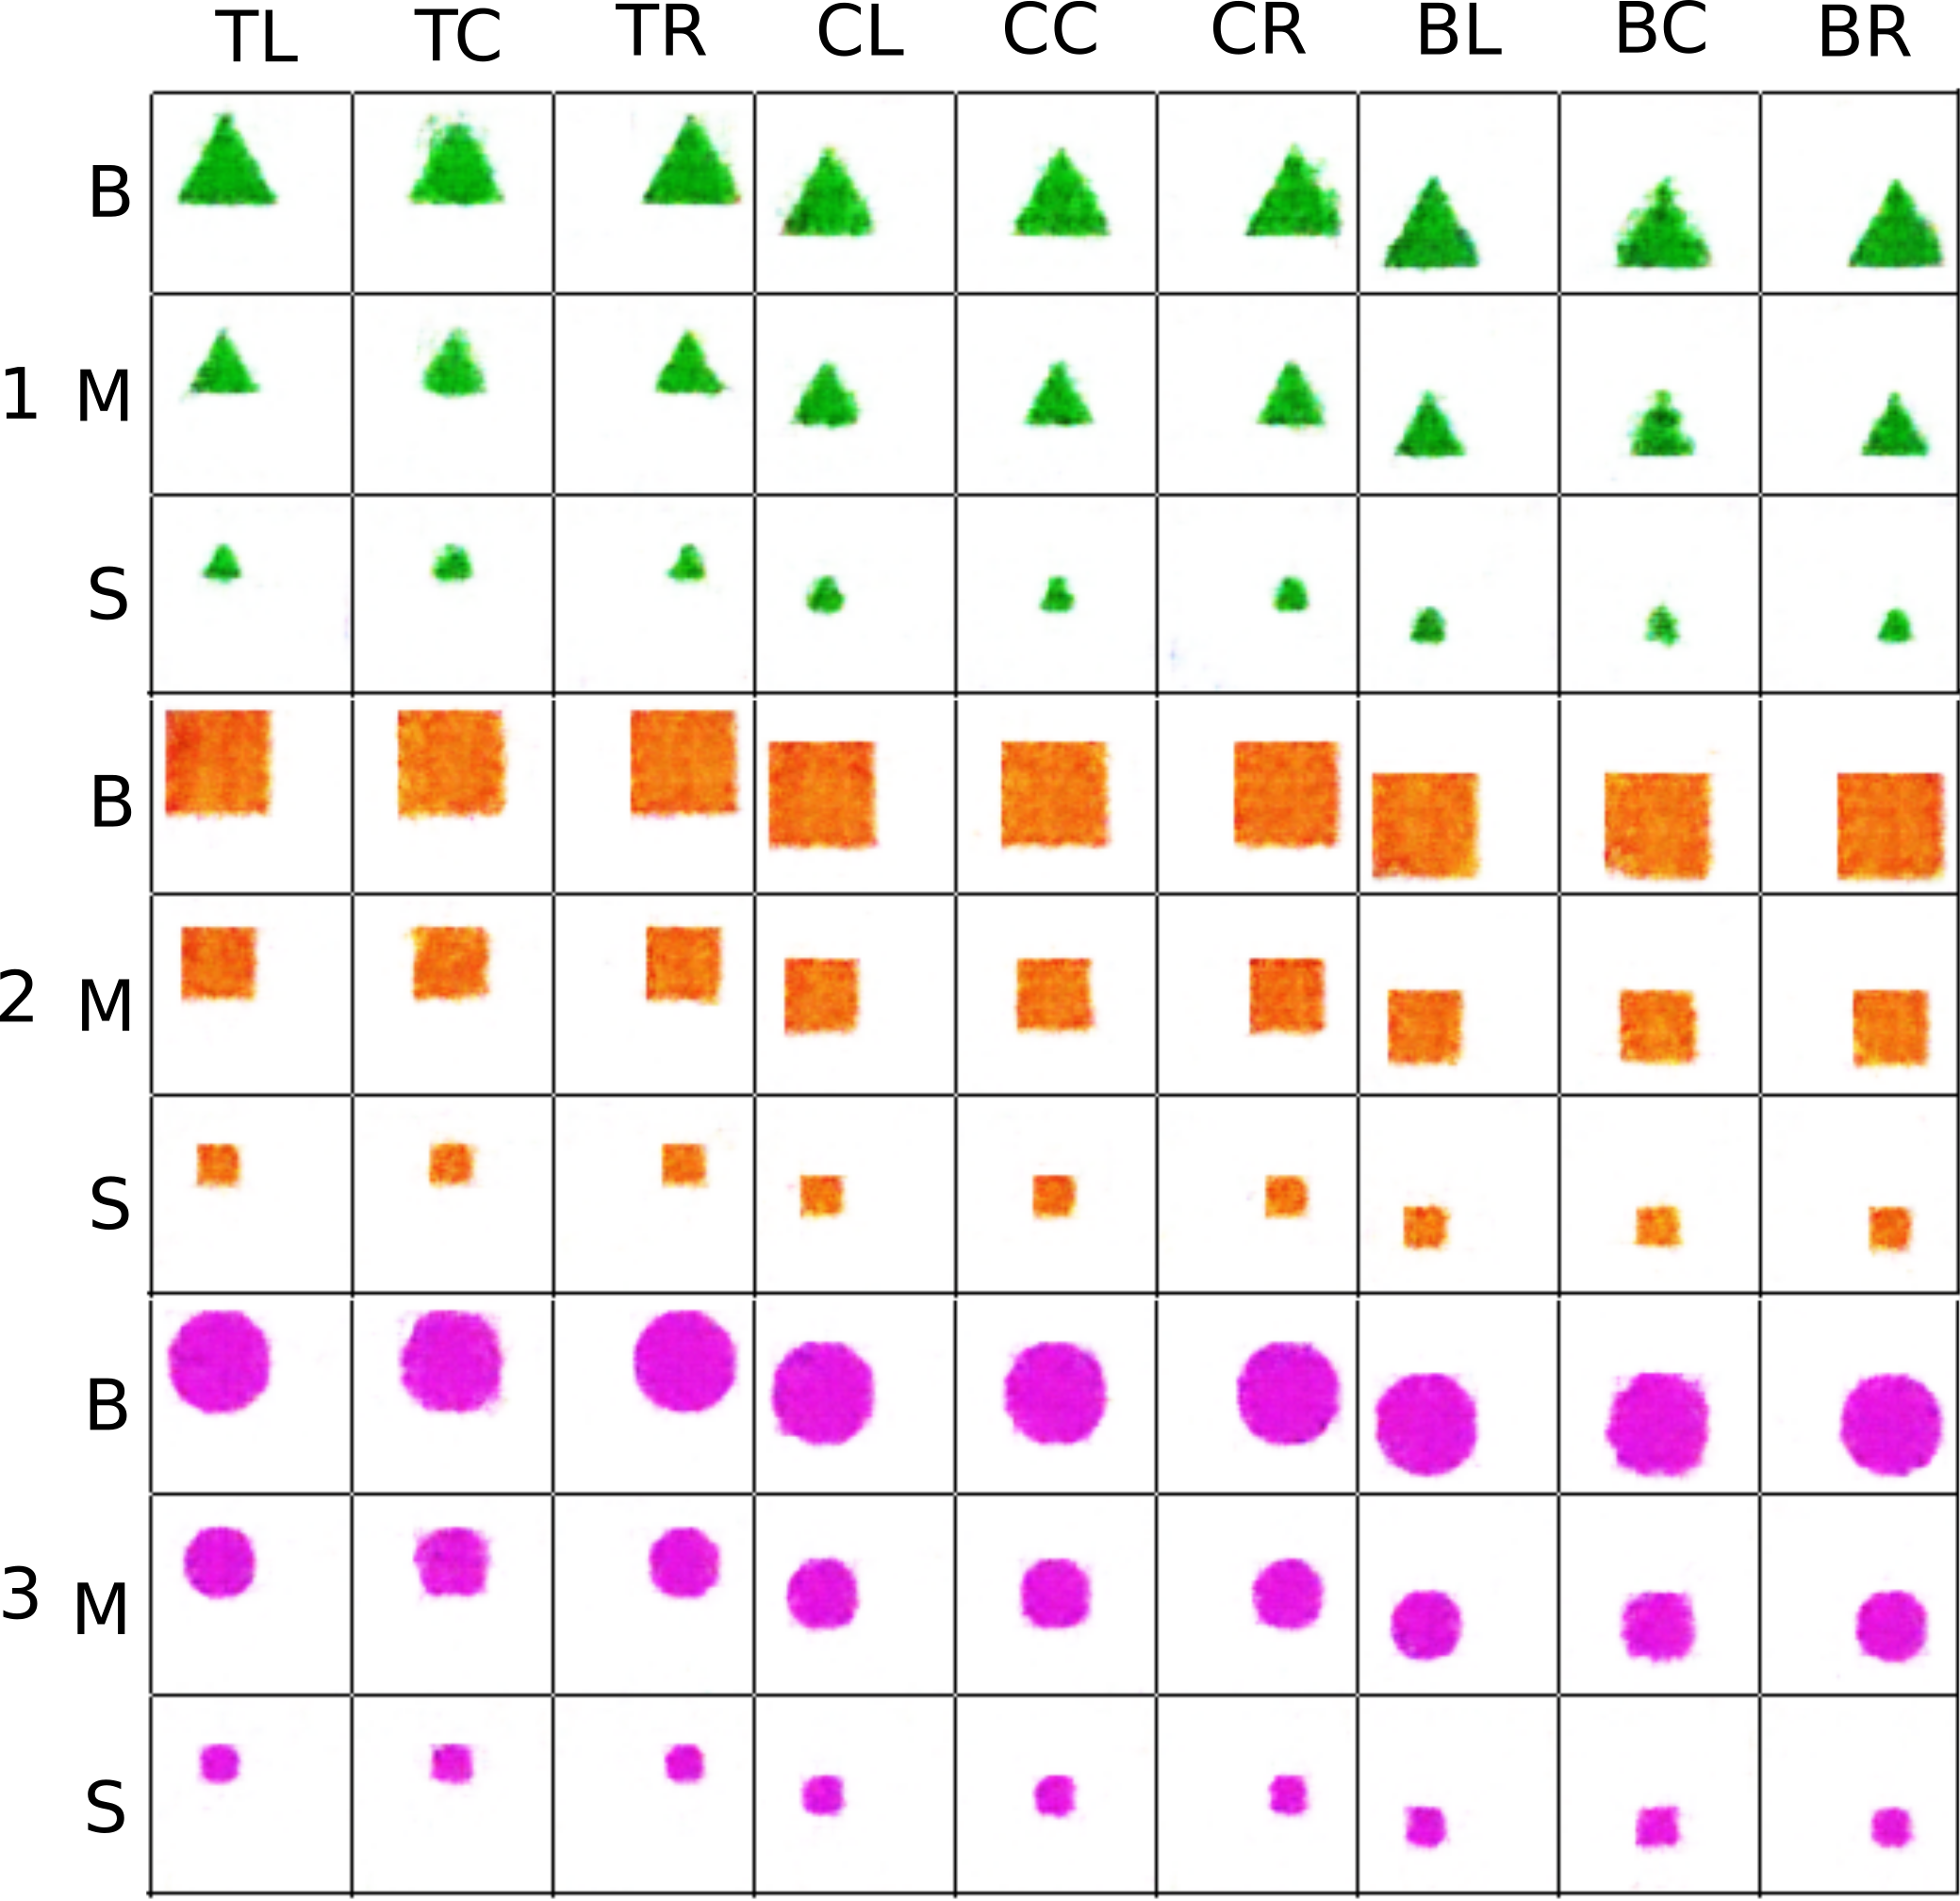
\includegraphics[width=0.5\textwidth]{Figs/shapes/739_minus1.png}
\caption{Experiment 5, run A: Images generated from descriptions of shapes never seen by the neural network.}
\label{fig:739_minus1}
\end{figure}

Despite never seeing a green triangle, MAE 1 from \autoref{fig:739_minus1} has learnt the meaning of each of the words \textsc{Triangle} and \textsc{Green} from instances of other coloured triangles and green circles and rectangles. A similar statment can be made about MAEs 2 and 3 in \autoref{fig:739_minus1}.

\begin{figure}[h]
\centering
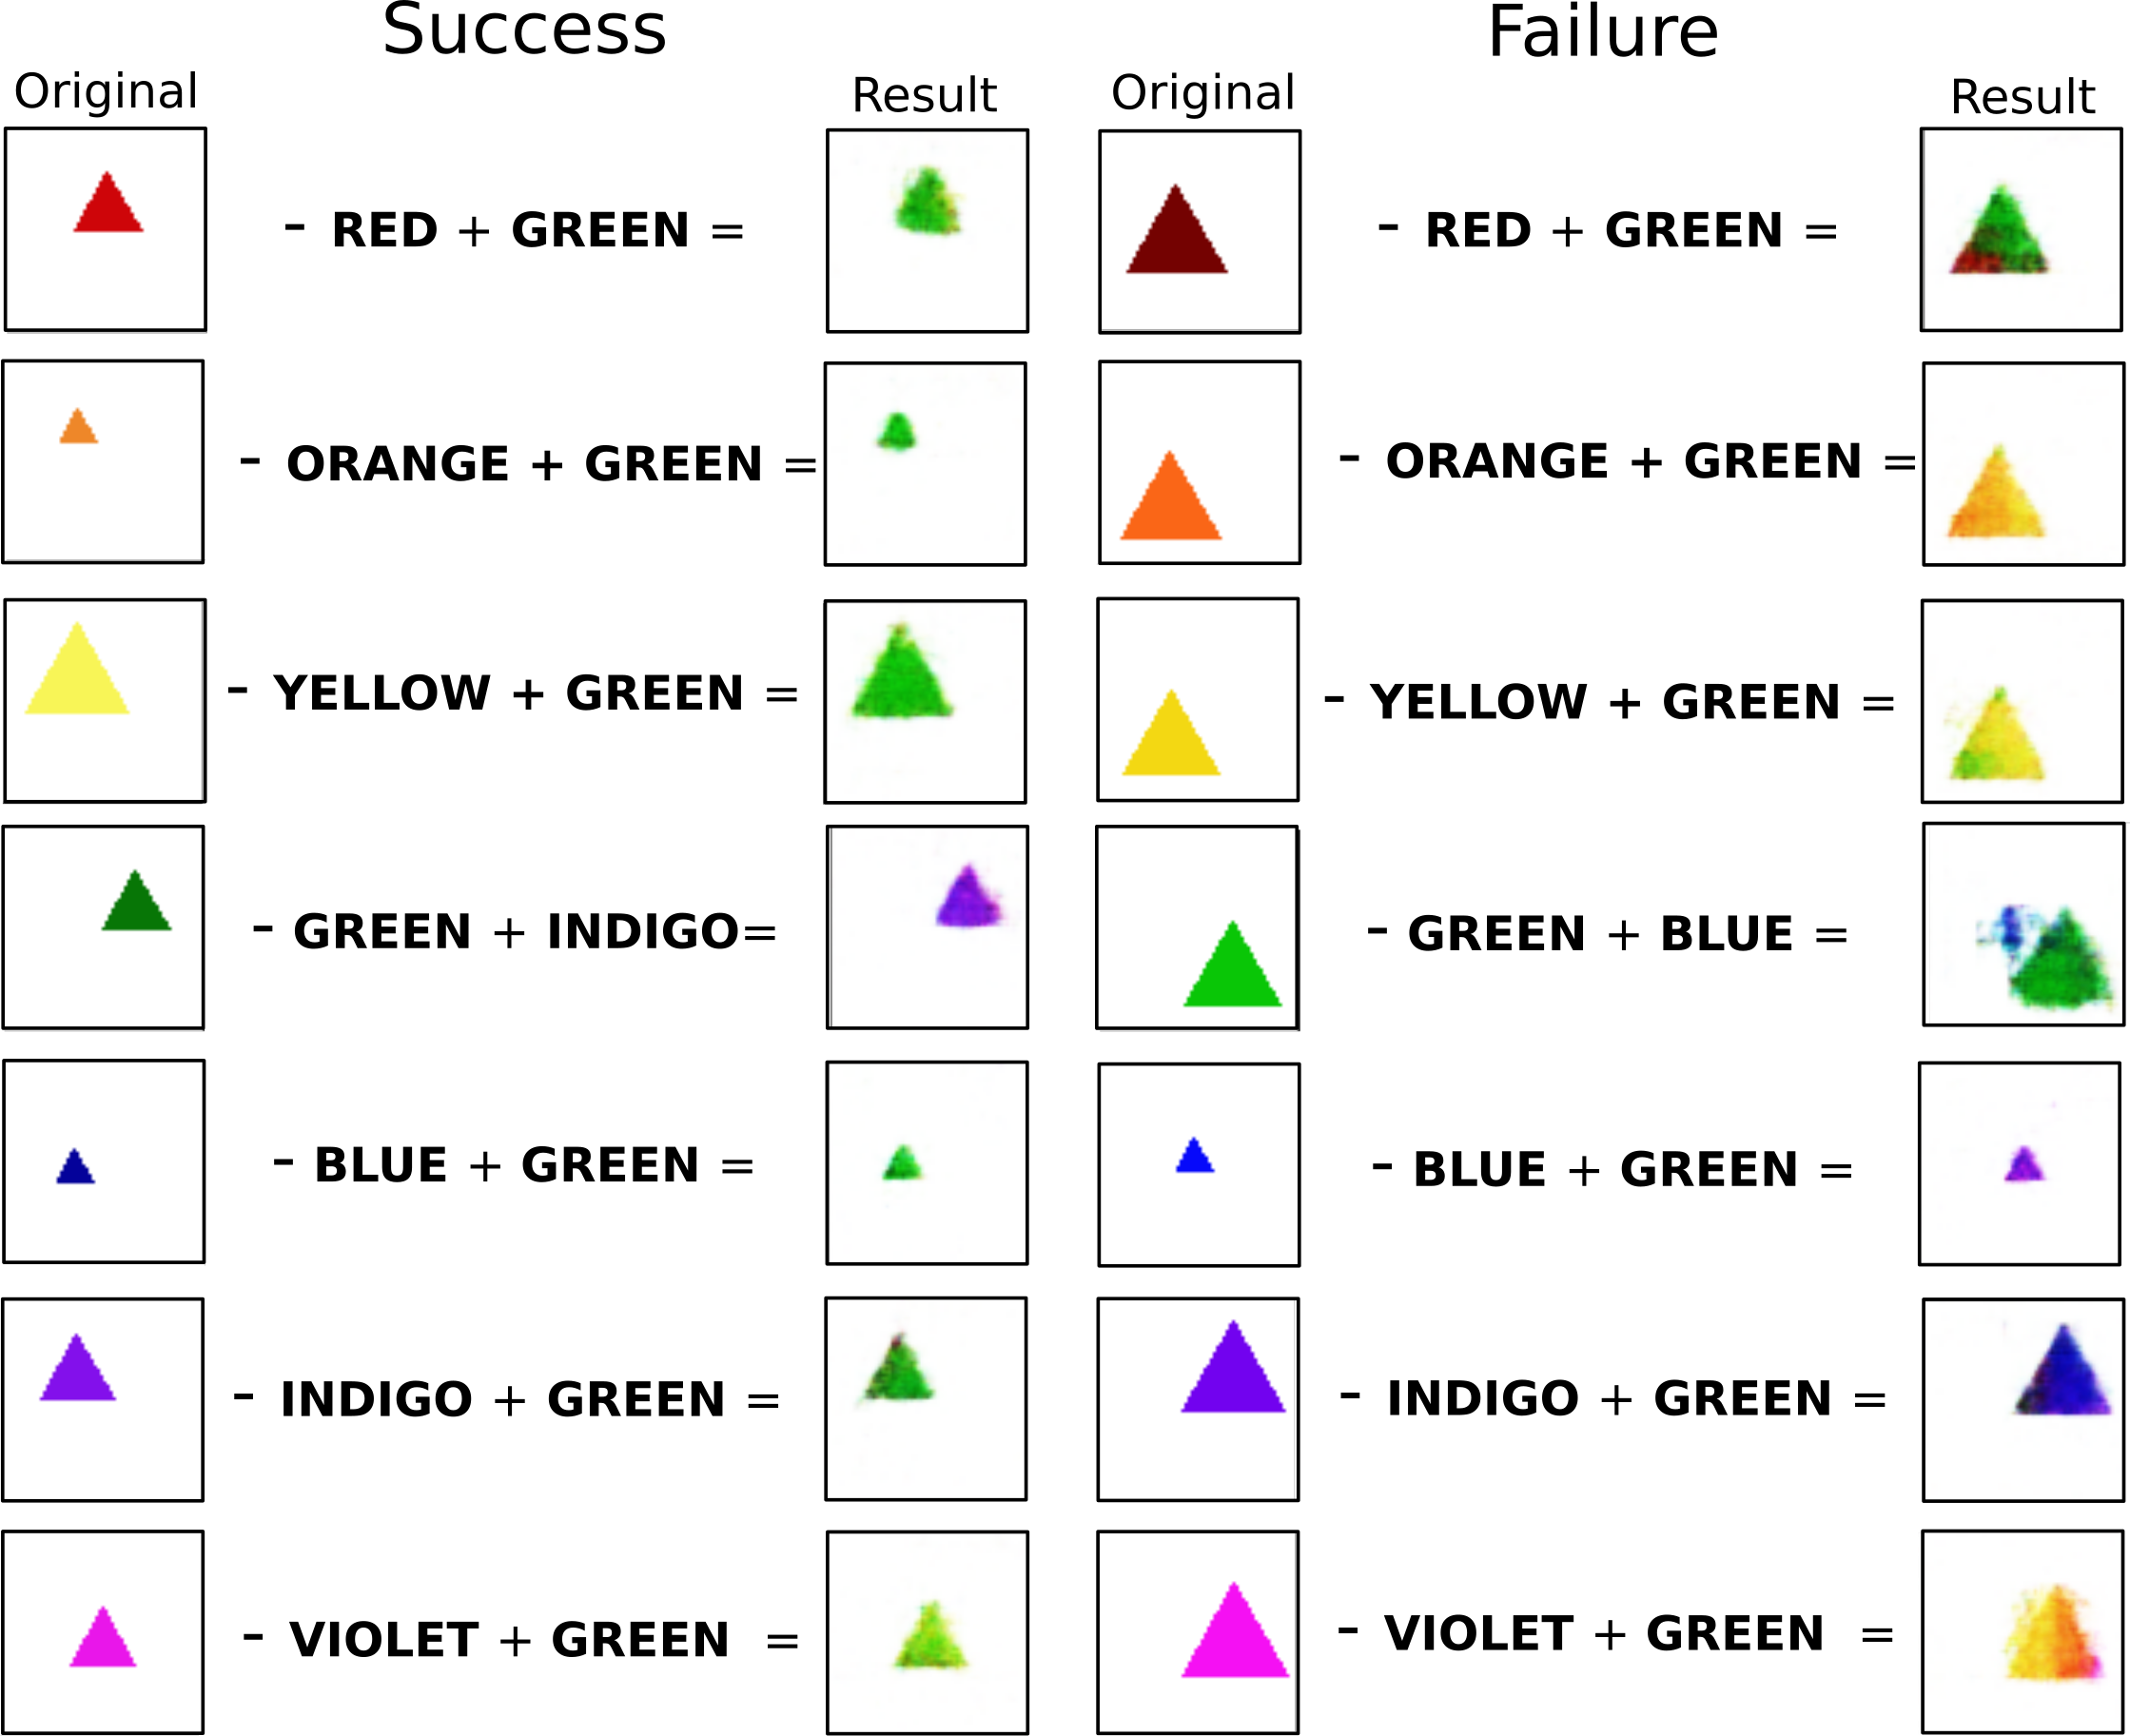
\includegraphics[width=0.75\textwidth]{Figs/shapes/739_minus1_vectorArthGT.png}
\caption{Experiment 5, run A: Images generated via Vector Arithmetic}
\label{fig:739_vectorArth}
\end{figure}

As explained earlier in this chapter, it is also possible to generate novel images by manipulating the embedding space of the neural network via Vector Arithmetic. \autoref{fig:739_vectorAth} shows a sample of images generated by MAE 1 (Results for MAEs 2 and 3 are in the supplemental material). Whilst some manipulations are successful for MAE 1, not all are. This is likely due to discontinuities in the latent embedding space. As the MAE has not been trained on every possible combination of colours, sizes, shapes and positions, there are parts of the embedding space it has never trained. This means that when vector arithmatic creates an embedding which lies in one of these unexplored areas, the MAE will not generate a sensible output. 

Comparing the MAEs from this experiment to images generated via Vector Arithmetic by the Exp 2 MAE from experiment 4, highlights this effect. The Exp 2 MAE had the best overall performance of any of the MAEs trained in this chapter and therefore it is unsurprising that it had the least discontinuities in its embedding space. The Exp 2 MAE did the best job of embedding the different words and visual attributes into the latent representation space, creating a smoother, more continuous representation space such that Vector Arithmetic was unlikely to lead to the generation of an embedding in an unexplored part of the representation space. 

\paragraph{Description Accuracy}
\begin{table}[h!]
\centering
	\begin{tabular}{|c|c|c|c|}
	\hline
Trial	 & 	Bimodal & 	Image Only 	& 	Words Only \\ \hline
MAE 1	&	99.99	$\mypm$	0.05	&	96.86	$\mypm$	7.10	&	100.00	$\mypm$	0.00	\\ \hline
MAE 1*	&	99.98	$\mypm$	0.10	&	92.54	$\mypm$	13.30	&	100.00	$\mypm$	0.00	\\ \hline
MAE 2	&	100.00	$\mypm$	0.00	&	99.03	$\mypm$	3.57	&	100.00	$\mypm$	0.00	\\ \hline
MAE 2*	&	99.97	$\mypm$	0.17	&	96.31	$\mypm$	10.065	&	99.68	$\mypm$	16.41	\\ \hline
MAE 3	&	100.00	$\mypm$	0.02	&	96.54	$\mypm$	7.71	&	100.00	$\mypm$	0.00	\\ \hline

MAE 3*	&	99.95	$\mypm$	0.32	&	92.27	$\mypm$	17.55	&	100.00	$\mypm$	0.00	\\ \hline

	\end{tabular}
\caption{Experiment 5: Percentage Description Accuracy. Alternating rows show accuracy for the datasubset without the omitted data and MSE for only the omitted data (marked with *)}
\label{tab:res_exp5_acc}
\end{table}

The MAEs are still able to accurately describe images of objects which appeared in the training data. However, they are also able to describe the images of the objects which were omitted from the training data. The MAEs have grounded the meanings of the all visual attributes, regardless of having some combinates excluded from the training data (e.g.\textit{Green Triangles}). There is an overall decrease in description accuracy for the omitted objects ($\approx 96 \% --> \approx 92 \%$). However for the non-omitted objects the performance is comparable to the accuracy of the random condition from experiment 4.

\subsubsection{Discussion}
Omitting one object from the training data has a minimal effect on the reconstruction of the other objects in the dataset, this can been by comparing the random initialisation condition from \autoref{tab:res739} and the results shown \autoref{tab:res_exp5}. This means that omitting one object, such as green triangles, does not affect the ability of the MAE to learn to ground the visual attributes \textit{Green} and \textit{Triangle} nor the words \textsc{Green} and \textsc{Triangle}. It can still generate green objects and triangles, approximately as well as the randomly initalised MAE from experiment 4.

This is further demonstrated by the MAEs ability to generate images of the unseen objects as shown in \autoref{fig:739_minus1}. As the MAE has grounded the meanings of the visual attributes \textit{Green} and \textit{Triangle} and the words \textsc{green} and \textsc{triangle}, it is able to combine their meansings to generate images of green triangles in different positions and sizes. (This is also true for orange rectangles and violet circles)

There is a negative effect on the reconstruction error for the ommited object and the labelling of the omitted object also suffers. Whilst labelling accuracy for objects types included in the training data generally remained very good (over 99\% in the image only testing condition), labelling of the omitted object was noticably worse, with an average of a 3.61\% reduction in accuracy across the three omitted objects.

Seeing that both accurate descriptions and reconstructed images can be generated by the MAE for unseen objects, we can conclude that the MAE is capable of bidirectional symbol grounding. This also highlights the effectivness and utility of this method. There is not a decrease in performance compared to the random condition of experiment 4, it is therefore possible that the MAE can be used to accuartely label unseen objects without a decrease in performance on seen objects.


\section{Conclusion}
I have demonstrated that utilising a MAE, it is possible to learn a multimodal representation of images and their descriptions. The embedding of images or descriptions into this representation can be used to generate novel descriptions or images.

Further to this, it is possible to directly manipulate the latent representation using vector arithmetic on embeddings from either modality making meaningful changes, generating images with altered visual attributes.

The learnt representation is very robust, even allowing for the generation of unseen combinations of words as images, or the descriptions of images of unseen objects. However, the quality of the representation is highly dependent on the data used for training and the training method used. The best results were achieved by first training on a subset of the data and then incrementally learning additional words and visual attributes.

The robustness of the representation is due to having bidirectionally grounded the meanings of words and visual attributes. For example, once the MAE has learnt the meaning of a word or visual attribute, combining it with other words or visual attributes generates a sensible output, regradless of whether that exact combination of words and visual attributes has been seen in the training data.

\subsubsection{How an incremental approach helps}
It might seem that the task of learning to bidirectionally ground the words of the descriptions and the visual attributes of the images is trivial. Of course, it is for an adult human. Even if the descriptions were given in an unknown language, given very few examples (possibly even less than one example per object) an adult could learn the relationship very quickly. Why then, does a neural network need so many examples to get things right?

The root of this issue comes down to two main factors, 1) the underlying probability distribution of the data and 2) the learning method: gradient descent.

To understand what I mean by ``the underlying probability distribution of the data'' let us consider the simple example of rolling a die to decide if it is fair.

How many times should we roll the die before we decide if it is fair? If it is a six sided die and it is fair, there should be a $\frac{1}{6}$ chance of rolling each of the numbers 1 to 6. So if we roll it 6 times we should expect to see each number once. However, we most likely won't, that doesn't mean our die is rigged.

As we roll the die more and more times, we can get a better understanding of the true probability of rolling a given number and therefore get closer to deciding if the die is indeed fair.

\begin{table}[h]
\centering
	\begin{tabular}{|c|c|c|c|c|c|c|}
	\hline
	Rolls & 1 & 2 & 3 & 4 & 5 & 6 \\ \hline
	10 & 0 & 0.2 & 0.2 & 0.3 & 0.2 & 0.1 \\ \hline
	1000 & 0.168 & 0.148 & 0.169 & 0.174 & 0.172 & 0.169  \\ \hline
	100000 & 0.166 & 0.166 & 0.167 & 0.168 & 0.165 & 0.167  \\ \hline
	1000000 & 0.167 & 0.167 & 0.167 & 0.167 & 0.167 & 0.167  \\ \hline
	\end{tabular}
	\caption{Probability distributions generated from rolling a 6 sided die.}
	\label{tab:dieProb}
\end{table}

As we roll the die more and more we will get closer to the actual probability distribution which governs its behaviour. In the limit, the probability for rolling any number should converge to $\frac{1}{6} = 0.167$. Looking at \autoref{tab:dieProb} we can see that the pseudo random number generator (PRNG) I used to simulate rolling a die on my computer, is probably mostly fair. 

So, how does this relate to the ArtS dataset? Let us replace rolling a die in this example with selecting random images from the ArtS dataset and ask, how much information does a set of samples tell us about the underlying distribution of the dataset. As we only select a finite number of images, we cannot capture the entire underlying distribution of the data. Therefore when we train a neural network, we will have an inaccuracte idea of the cost landscape.

Given how gradient descent works, as explained in \autoref{Chapter3},  minimising the cost until it reaches a minimum, if we have an incomplete picture of the cost landscape, it is likely that gradient descent will get stuck in a local minimum, and not find the global minimum.

As it isn't feasible to provide infinite training examples to allow the neural network to get a complete picture of the cost landscape, we must find someway of constraining the cost landscape instead.

Let us consider two scenarios, 1) we sample data for a relatively complex task (like in experiment 4) and start from random weights, 2) we pretrain on a simpler task, then sample data for the more complex task (like in experiment 4 training from the weights learnt in experiment 2).

If we draw the cost landscapes in these two scenarios as well as the true cost landscape, we might get a figure like \autoref{fig:localminima}. The ``sampled cost'' relates to starting from random weights and the ``pretrained cost'' is the estimated cost landscape based on the data seen during pretraining.
\begin{figure}[h!]
\begin{center}
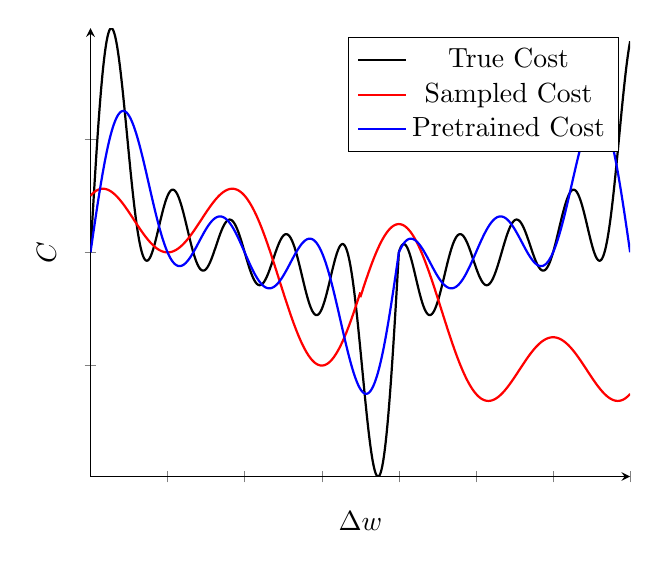
\begin{tikzpicture}
\begin{axis}[
axis lines=left,
xtick={90, 180, 270, 360,450,540,630},
xticklabels={},
xlabel={$\Delta w$},
ylabel={$C$},
yticklabels={},
xlabel near ticks,
ylabel near ticks]
\addplot[black, thick, smooth, samples=1000, domain=0:360]{sin(x) + sin(2*\x)+sin(3*\x)+sin(4*\x) + sin(5*\x)};

\addplot[black, thick, smooth, samples=1000, domain=360:630]{-sin(1*(\x-300)) -sin(2*(\x-300)) -sin(3*(\x-300)) -sin(4*(\x-300)) -sin(5*(\x-300))};




\addplot[red, thick, smooth, samples=1000, domain=0:315]{-cos(1*(\x-270)) -cos(2*(\x-270)) };

\addplot[red, thick, smooth, samples=1000, domain=315:630]{(-cos(\x-180) + -cos(2*\x-180))-1.50};


\addplot[blue, thick, smooth, samples=1000, domain=0:360]{sin(x) + sin(2*\x)+sin(3*\x)};

\addplot[blue, thick, smooth, samples=1000, domain=360:630]{-sin(1*(\x-270)) -sin(2*(\x-270)) -sin(3*(\x-270))};


\node [red] at (470,130)  (a) {\textbullet};
\node [black] at (335,5)  (a) {\textbullet};
\node [blue] at (320,145) (b) {\textbullet};
\legend{True Cost, , Sampled Cost, , Pretrained Cost, }
\end{axis}
    

\end{tikzpicture}
\caption{Visualisation of an imaginary Error landscape.}
\label{fig:localminima}
\end{center}
\end{figure}

Consider the red point on the red line shown in \autoref{fig:localminima}, this represents the minimum of the cost landscape estimate from sampling data for a task without performing pretraining on a simplier task. It is possible that the weights of the neural network will get stuck in the local minima. This is essentially over fitting the data due to having an unconstrained search space and limited knowledge of the cost landscape.

If we pretrain, allowing the network to first master a simpler task, the estimate of the true cost landscape will be different as it is based off of the data sampled in the simpler task. In \autoref{fig:localminima} this is represented by the blue line. As we know that the neural network performs well on the simpler task, we can reason that it is likely the weights of the network are relatively close to the global optimum before training on the data sampled for the more complex task.


When we pretrain using a different subset of the data as in experiments 3 and 4, we start at a point in the cost landscape that is hopefully closer to the global minima than starting with randomly selected weights. Obviously, this is not always the case, for example, only pretraining on experiment 2 helped in both experiments 3 and 4. Pretraining on experiment 1 did not have a positive effect on the bidirectional symbol grounding.

So, by taking a incremental approach, mastering simple tasks and increasing the difficulty of the tasks we set our neural networks to tackle, we can incrementally approach the global cost minima. In the case of the ArtS dataset this means incrementally learning to perform bidirectional symbol grounding on a wider variety of words and visual properties. Learning new colours, shapes, sizes and positions. As we saw from the results of experiment 4, this approach can lead to better performance than simply training longer on the more difficult task.



 
%% Chapter Template

\chapter{Bidirectional Grounding of Real Data} % Main chapter title

\label{Chapter6} % Change X to a consecutive number; for referencing this chapter elsewhere, use \ref{ChapterX}

\lhead{Chapter 6. \emph{Bidirectional Grounding of Real Data}} % Change X to a consecutive number; this is for the header on each page - perhaps a shortened title

%----------------------------------------------------------------------------------------
%	SECTION 1
%----------------------------------------------------------------------------------------
\section{The Difficulties of Real Data}
In the previous chapter I showed that it is possible to use a \ac{MAE} to bidirectionally ground natural language (words) and the visual attributes of images of different objects through \ac{MRL}. However, the data used in the previous chapter is artificial and therefore many of the challenges which real data presents are not present in it. 

When working with real images, there are many factors to consider such as lighting changes, perspective changes and camera noise \cite{keller2016analysis}. These factors were not present in the ArtS dataset, so in this chapter I will show how these impact \ac{MRL} for bidirectional grounding.



\begin{figure}[h]
    \centering
    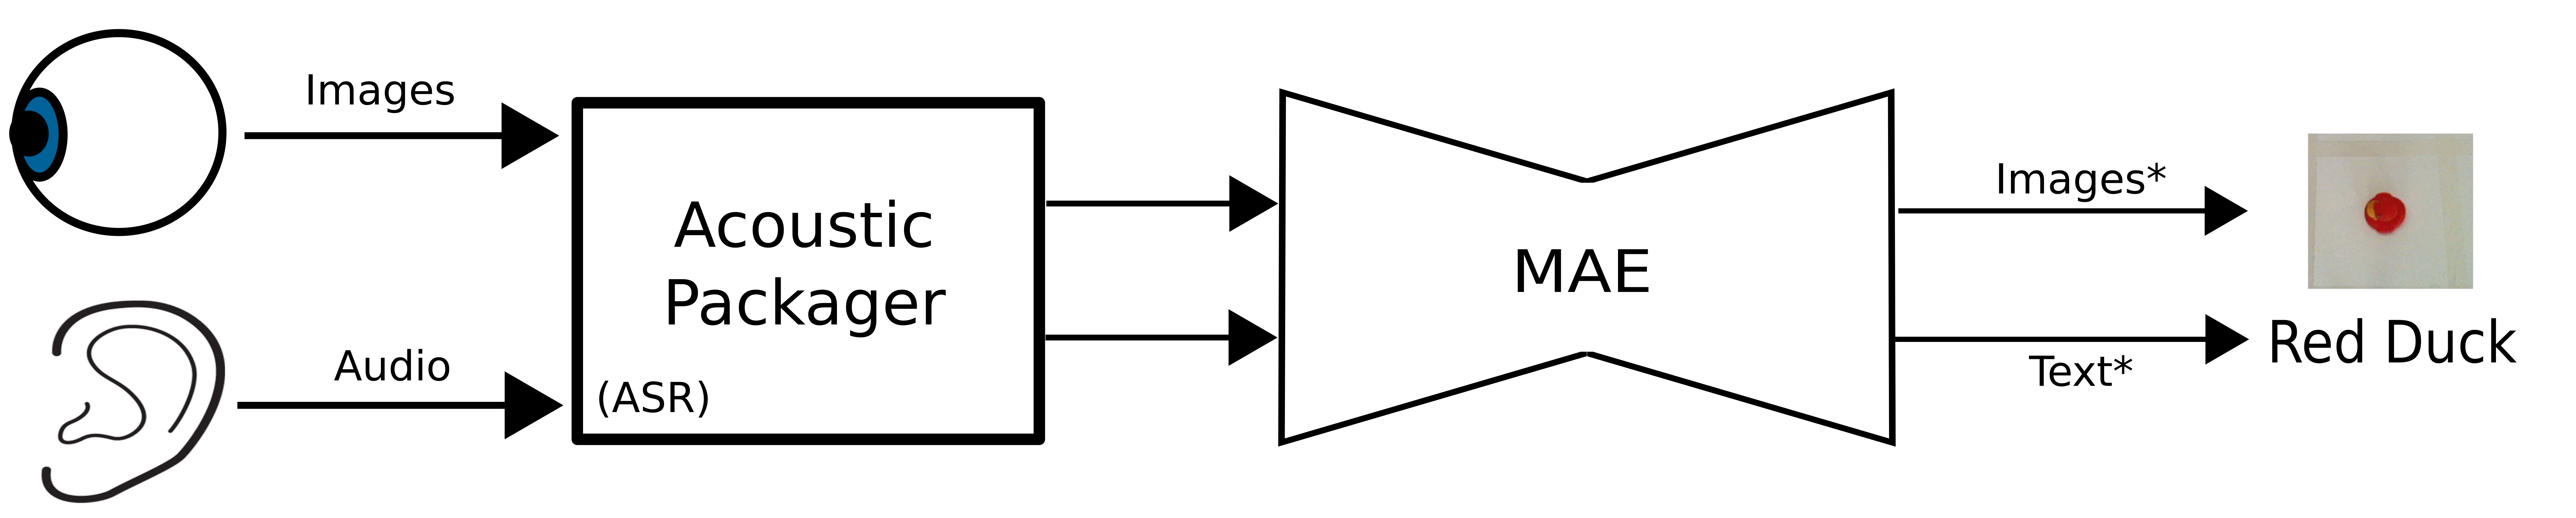
\includegraphics[width=0.7\textwidth]{Figs/chapter6/bimodal_system_schematic.png}
    \caption{System schematic. Data is captured from sensors by an acoustic packager and fed to the multimodal autoencoder.}
    \label{fig:schematic}
\end{figure}

\section{Acoustic Packaging}
In order to make use of \ac{MRL} on a robot, it is necessary to have a method to gather and group data from multiple sensory modalities. To do this, I make use of \ac{AP} \cite{schillingmann2009towards, schillingmann2009computational}.

The acoustic packager I implemented for this, is triggered to capture data when sound above a certain threshold is heard by a microphone. Images and audio are recorded with the audio being passed to an \ac{ASR} system to transcribe any speech. The audio, transcription and image together are refered to as an acoustic-package.

I do not make use of the audio, I use only the transcribed text and images such that the data used in this chapter is analigous to the data used in the previous chapter.

\section{Real Shapes Dataset}

\begin{figure}[h]
    \centering
    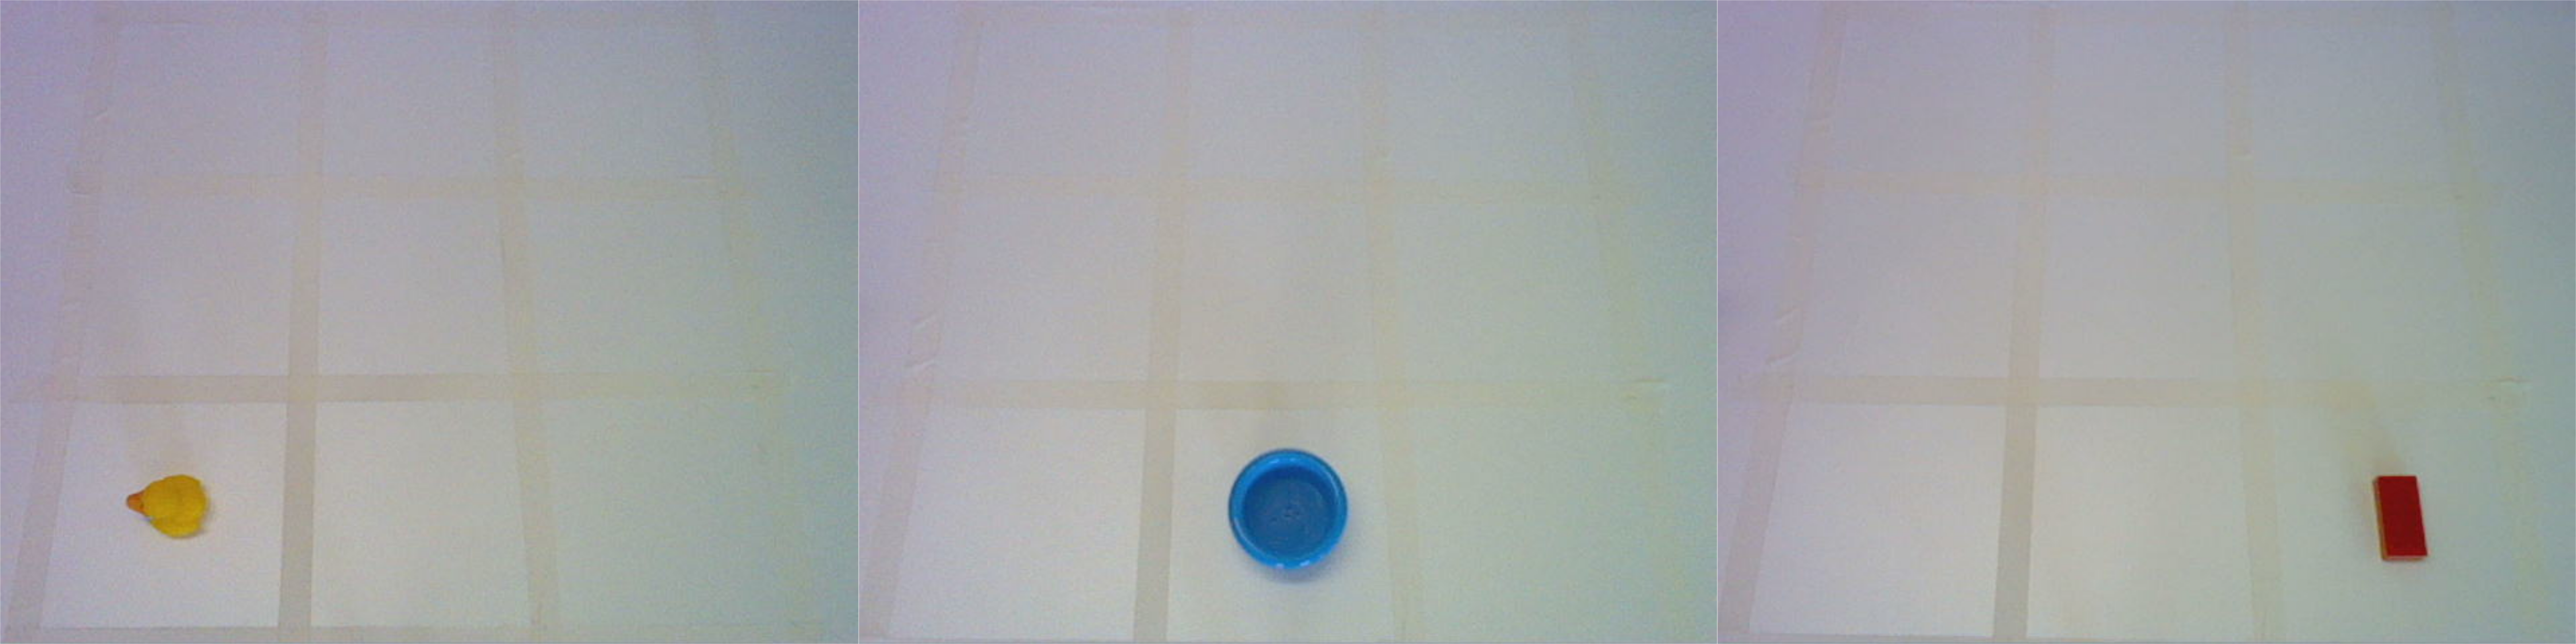
\includegraphics[width=\textwidth]{Figs/chapter6/ReShapeExs.png}
    \caption{Example images from ReShape.}
    \label{fig:ReShape}
\end{figure}

The Real Shapes dataset (ReShape) was created by presenting various objects to a webcam in 9 different positions and giving a short description of the object. \autoref{fig:ReShape} shows example images from ReShape.

\subsection{Dataset Description}
The ReShape dataset contains images and short descriptions of the images.

There are 7 objects, in 10 colours and 3 sizes. Not all objects appear in all 10 colours or all 3 sizes.

\autoref{fig:ReShapeAll} shows cropped, exemplar images for all objects in the ReShape dataset. Not all shape-colour-size combinations are covered in the dataset, hence the large number of blank spaces.

\newpage
\begin{figure}[h!]
    \centering
    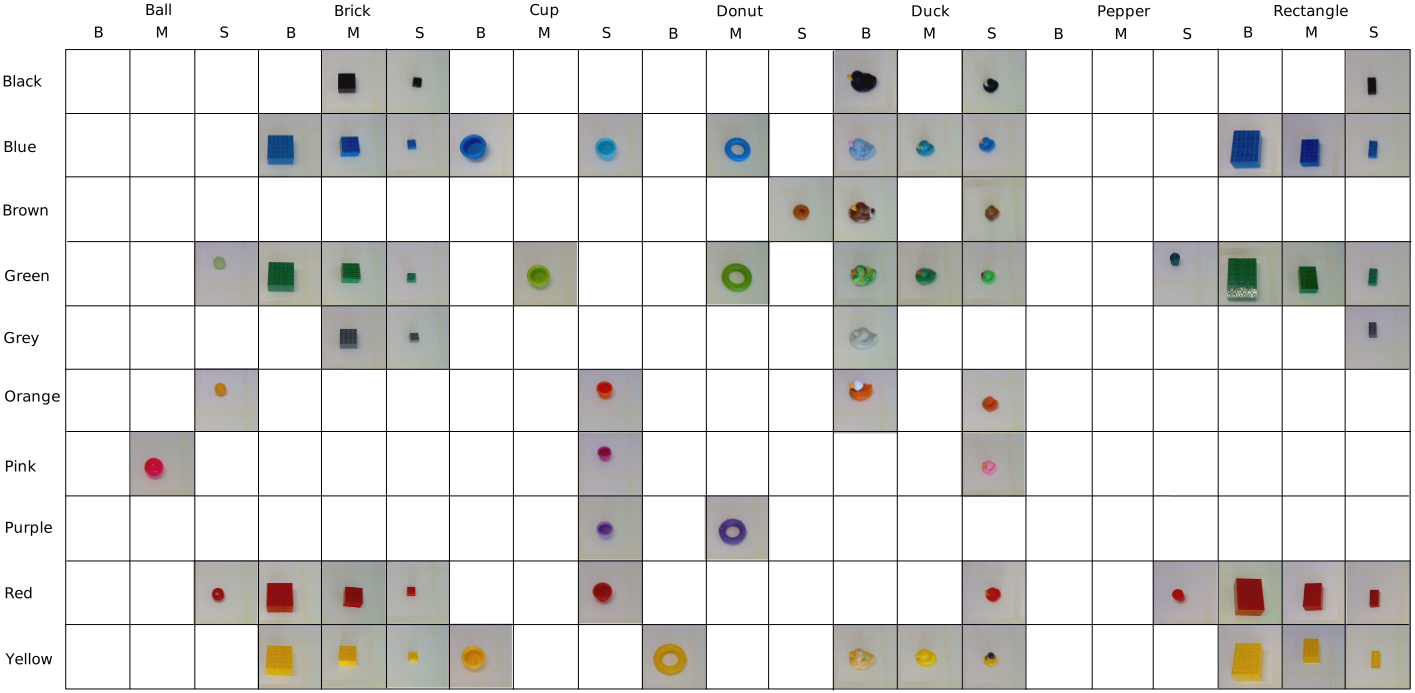
\includegraphics[height=0.7\textwidth, angle=90]{Figs/chapter6/ExemplarAllClasses.png}
    \caption{Exemplar images for all objects in the ReShape dataset.}
    \label{fig:ReShapeAll}
\end{figure}

The dataset was captured in several sessions across multiple days. This is the main source of vairability in the dataset, as different lighting conditions due to weather and time of day has a significant affect on the appearance of images captured by digital cameras \cite{keller2016analysis, keller}\endnote{In \autoref{fig:ReShapeCrop} differences in the lighting conditions are clearly visible with the top left and top centre image having a blue tint.}.


\subsection{Problem Description}
As in the previsous chapter I will be training \acp{MAE} to learn a joint embedding of images and their descriptions. The descriptions only contain a size, shape and colour and not a position as the images are cropped, centring the object in the image, the notion of position is removed from both modalities.

\subsection{Network Description}
I make use of the same network as used in chapter 5 with an embedding size of 296 neurons and a description output size of 13. \textcolor{red}{The network was not redesigned for this chapter as the task is very similar and the performance of this design was good in \autoref{chapter5}. \autoref{fig:netReShape} depicts the \ac{MAE} described in \autoref{tab:Arts_MAE_description}. The blue box shows the portion of the \ac{MAE} which encodes and decodes images, whilst the green portion encodes and decodes the descriptions. The orange box is where the joint representation is formed. Inputs are labelled, Image and Description with their respective outputs being marked with an asterisk. Whislt the overall structure of the \ac{MAE} used in this chapter is the same as that used in \autoref{Chapter5}, as the vocabulary size for the descriptions is smaller, the Description output layer only has 13 neurons unlike in \autoref{Chapter5} where the description output had 22 neurons.}

\begin{figure}
\centering
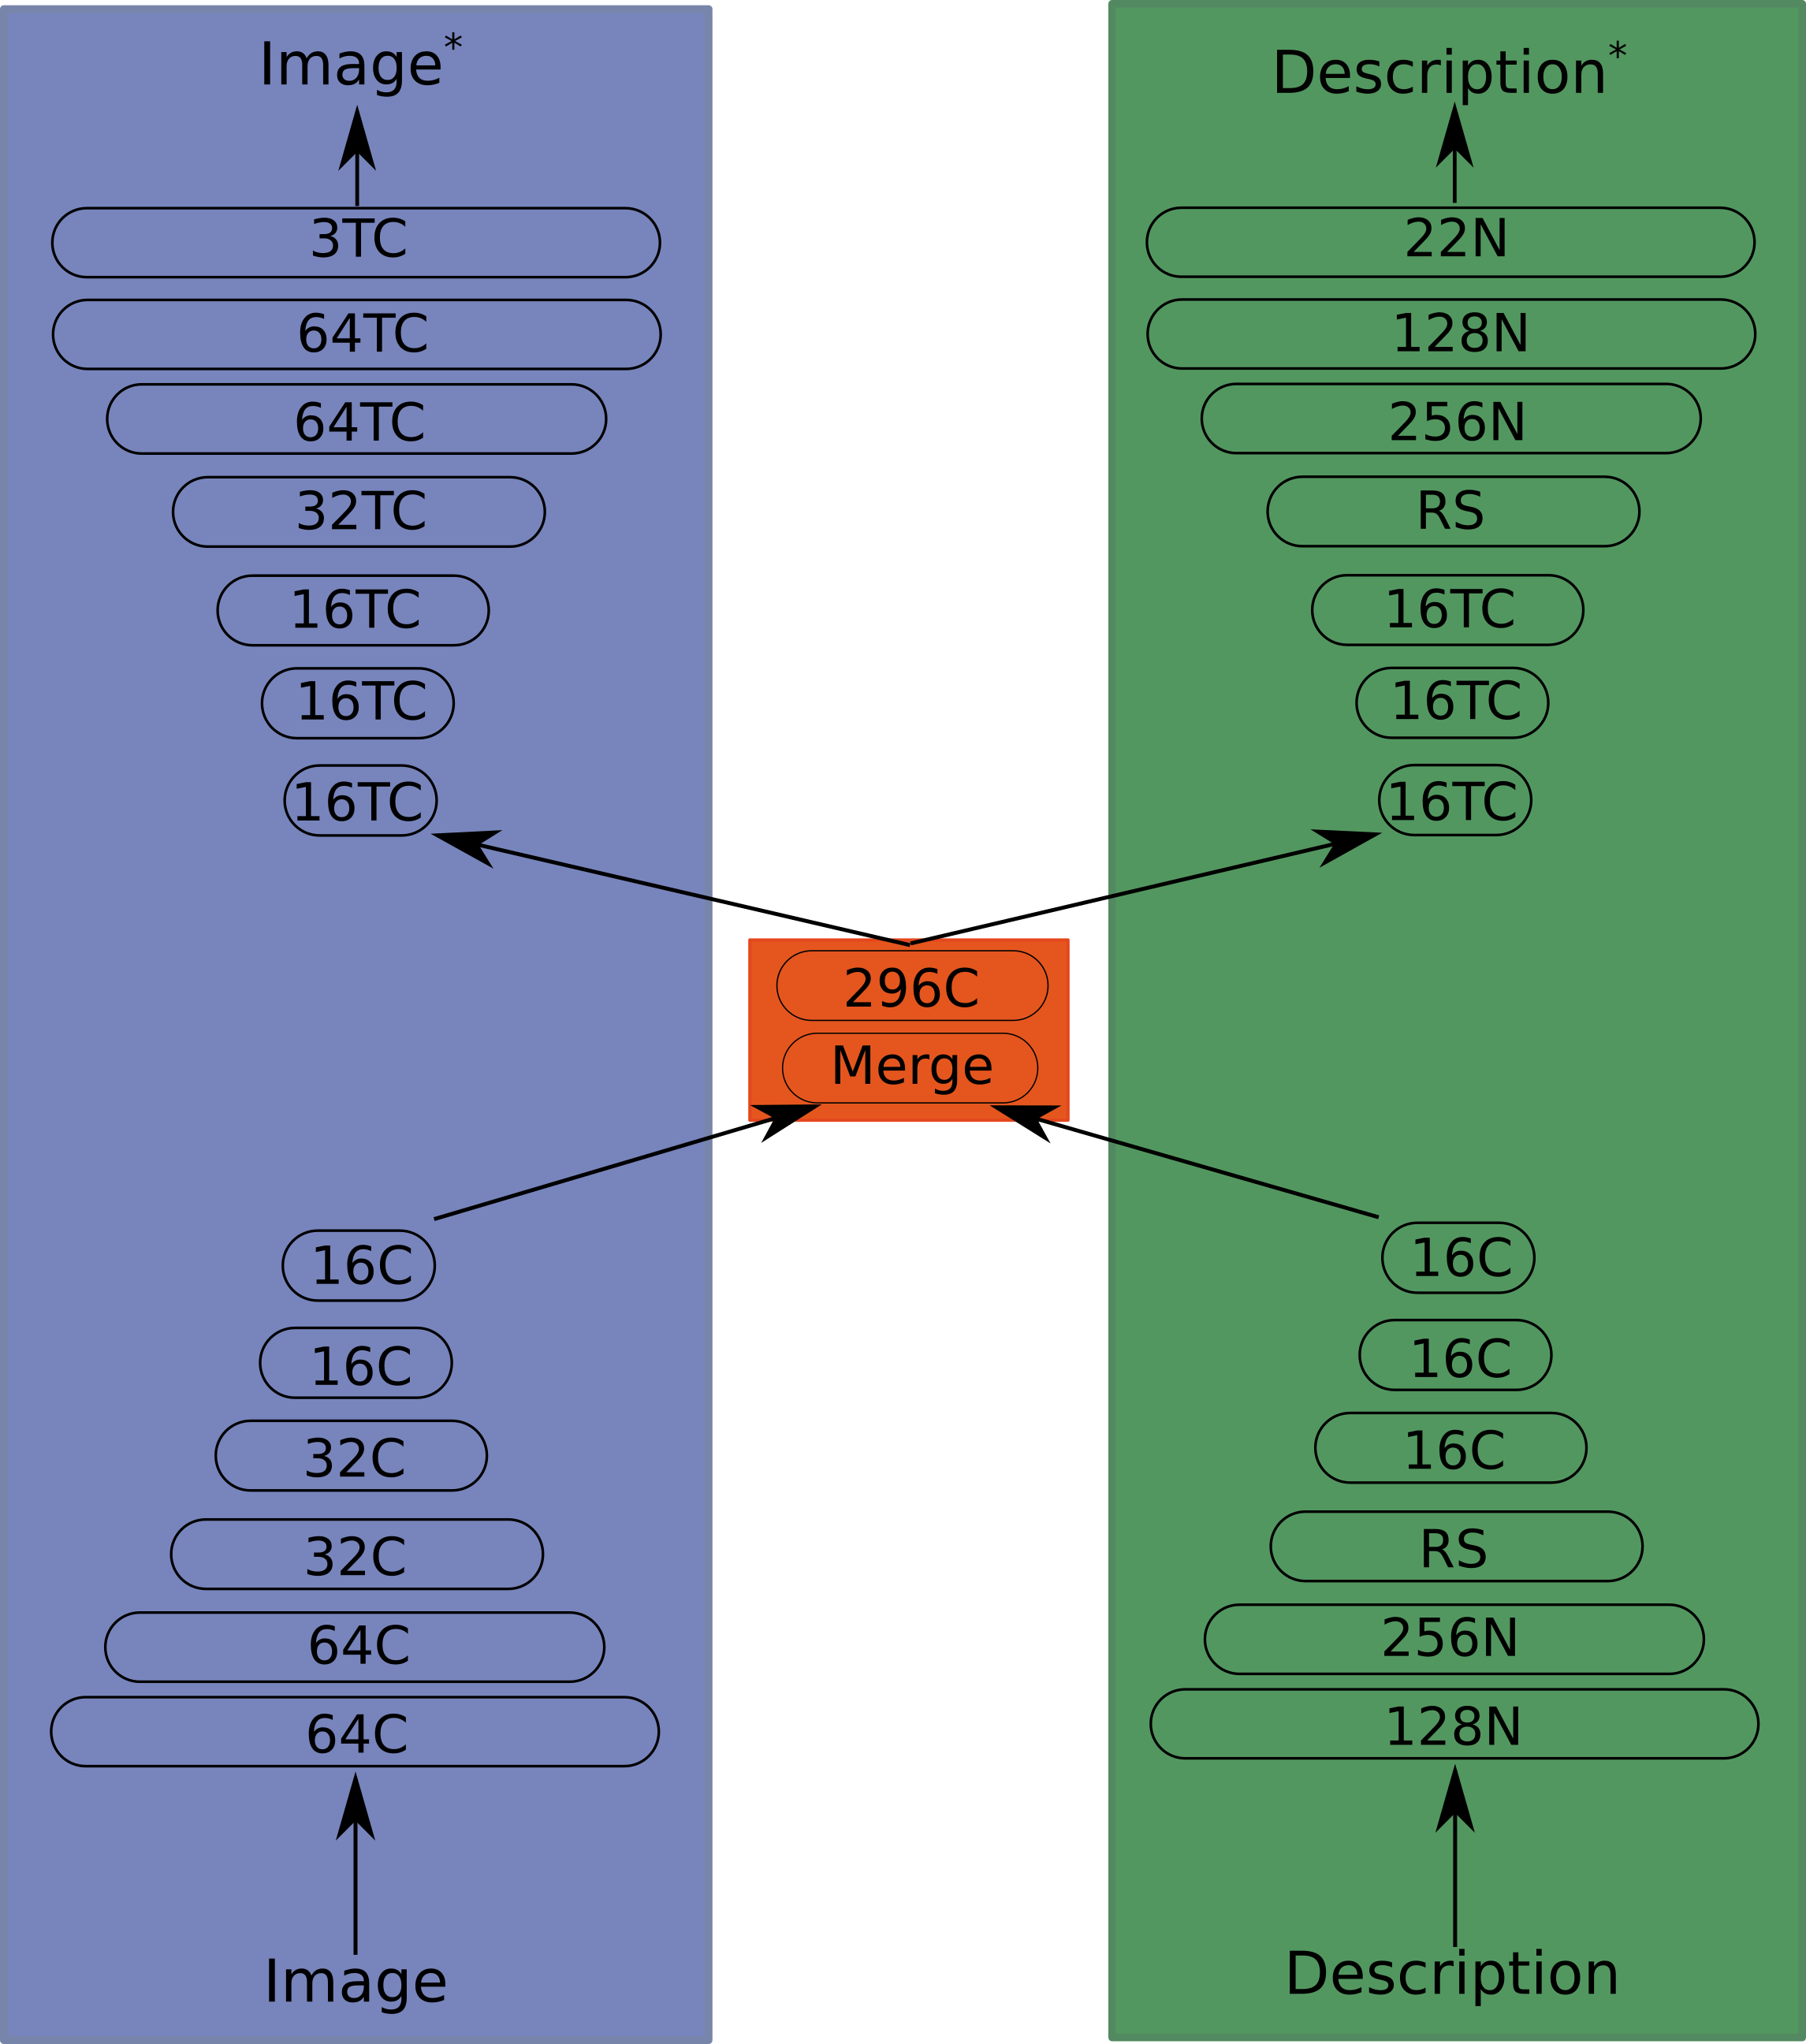
\includegraphics[width=0.75\textwidth]{Figs/shapes/maeArch.png}
\caption{\textcolor{red}{The \ac{MAE} architecture used in this chapters. Layers marked with C are convolution TC, Transposed Convolution, RS, Reshape and N, Dense.}}
\label{fig:netReShape}
\end{figure}



\section{Experiments with the ReShape dataset}
I perform two experiments, one with a small subset of the ReShape dataset where complete coverage of every trained and tested combination of colour, object and size is available. The second makes use of a larger variety of objects and colours, however not every combination of object, colour and size is available for training, thus there is not complete coverage, this is similar to experiment 5 in \autoref{Chapter5} where one object-colour combination was excluded from the training data. 

I will also look at the effect of pretraining on the data from experiment 1 and then training for experiment 2. Further to this, two training procedures will be introduced and compared, simple and exemplar.

\textcolor{red}{Both experiments test hypothesis 6: It is possible to use \ac{MRL} with real data. Beyond this, experiment 2 further explores hypothesis 5: The multimodal representation learnt by the \acp{MAE} exhibits all of the desirable properties of a representation as layed out by Bengio et al. in \cite{repRev}, by deomnstrating that the \ac{MAE} is able to cope with missing objects in the training data as the learnt representation exhibits manifolds and a degree of smoothness such that the individual symbols from which objects are constructed can be combined to generate images of unseen objects.}

\subsection{Data Preprocessing}

In the following experiments I do not consider the notion of position and instead crop each image so that the object is roughly centred and consider all objects of the same type to be the equivalent regardless of position (e.g. a \textsc{big blue duck top left} is considered the same as a \textsc{big blue duck center}). As such, the position word is removed from the description of the image and the \ac{MAE} does not contain the position words in its "vocabulary".

\begin{figure}[h]
    \centering
    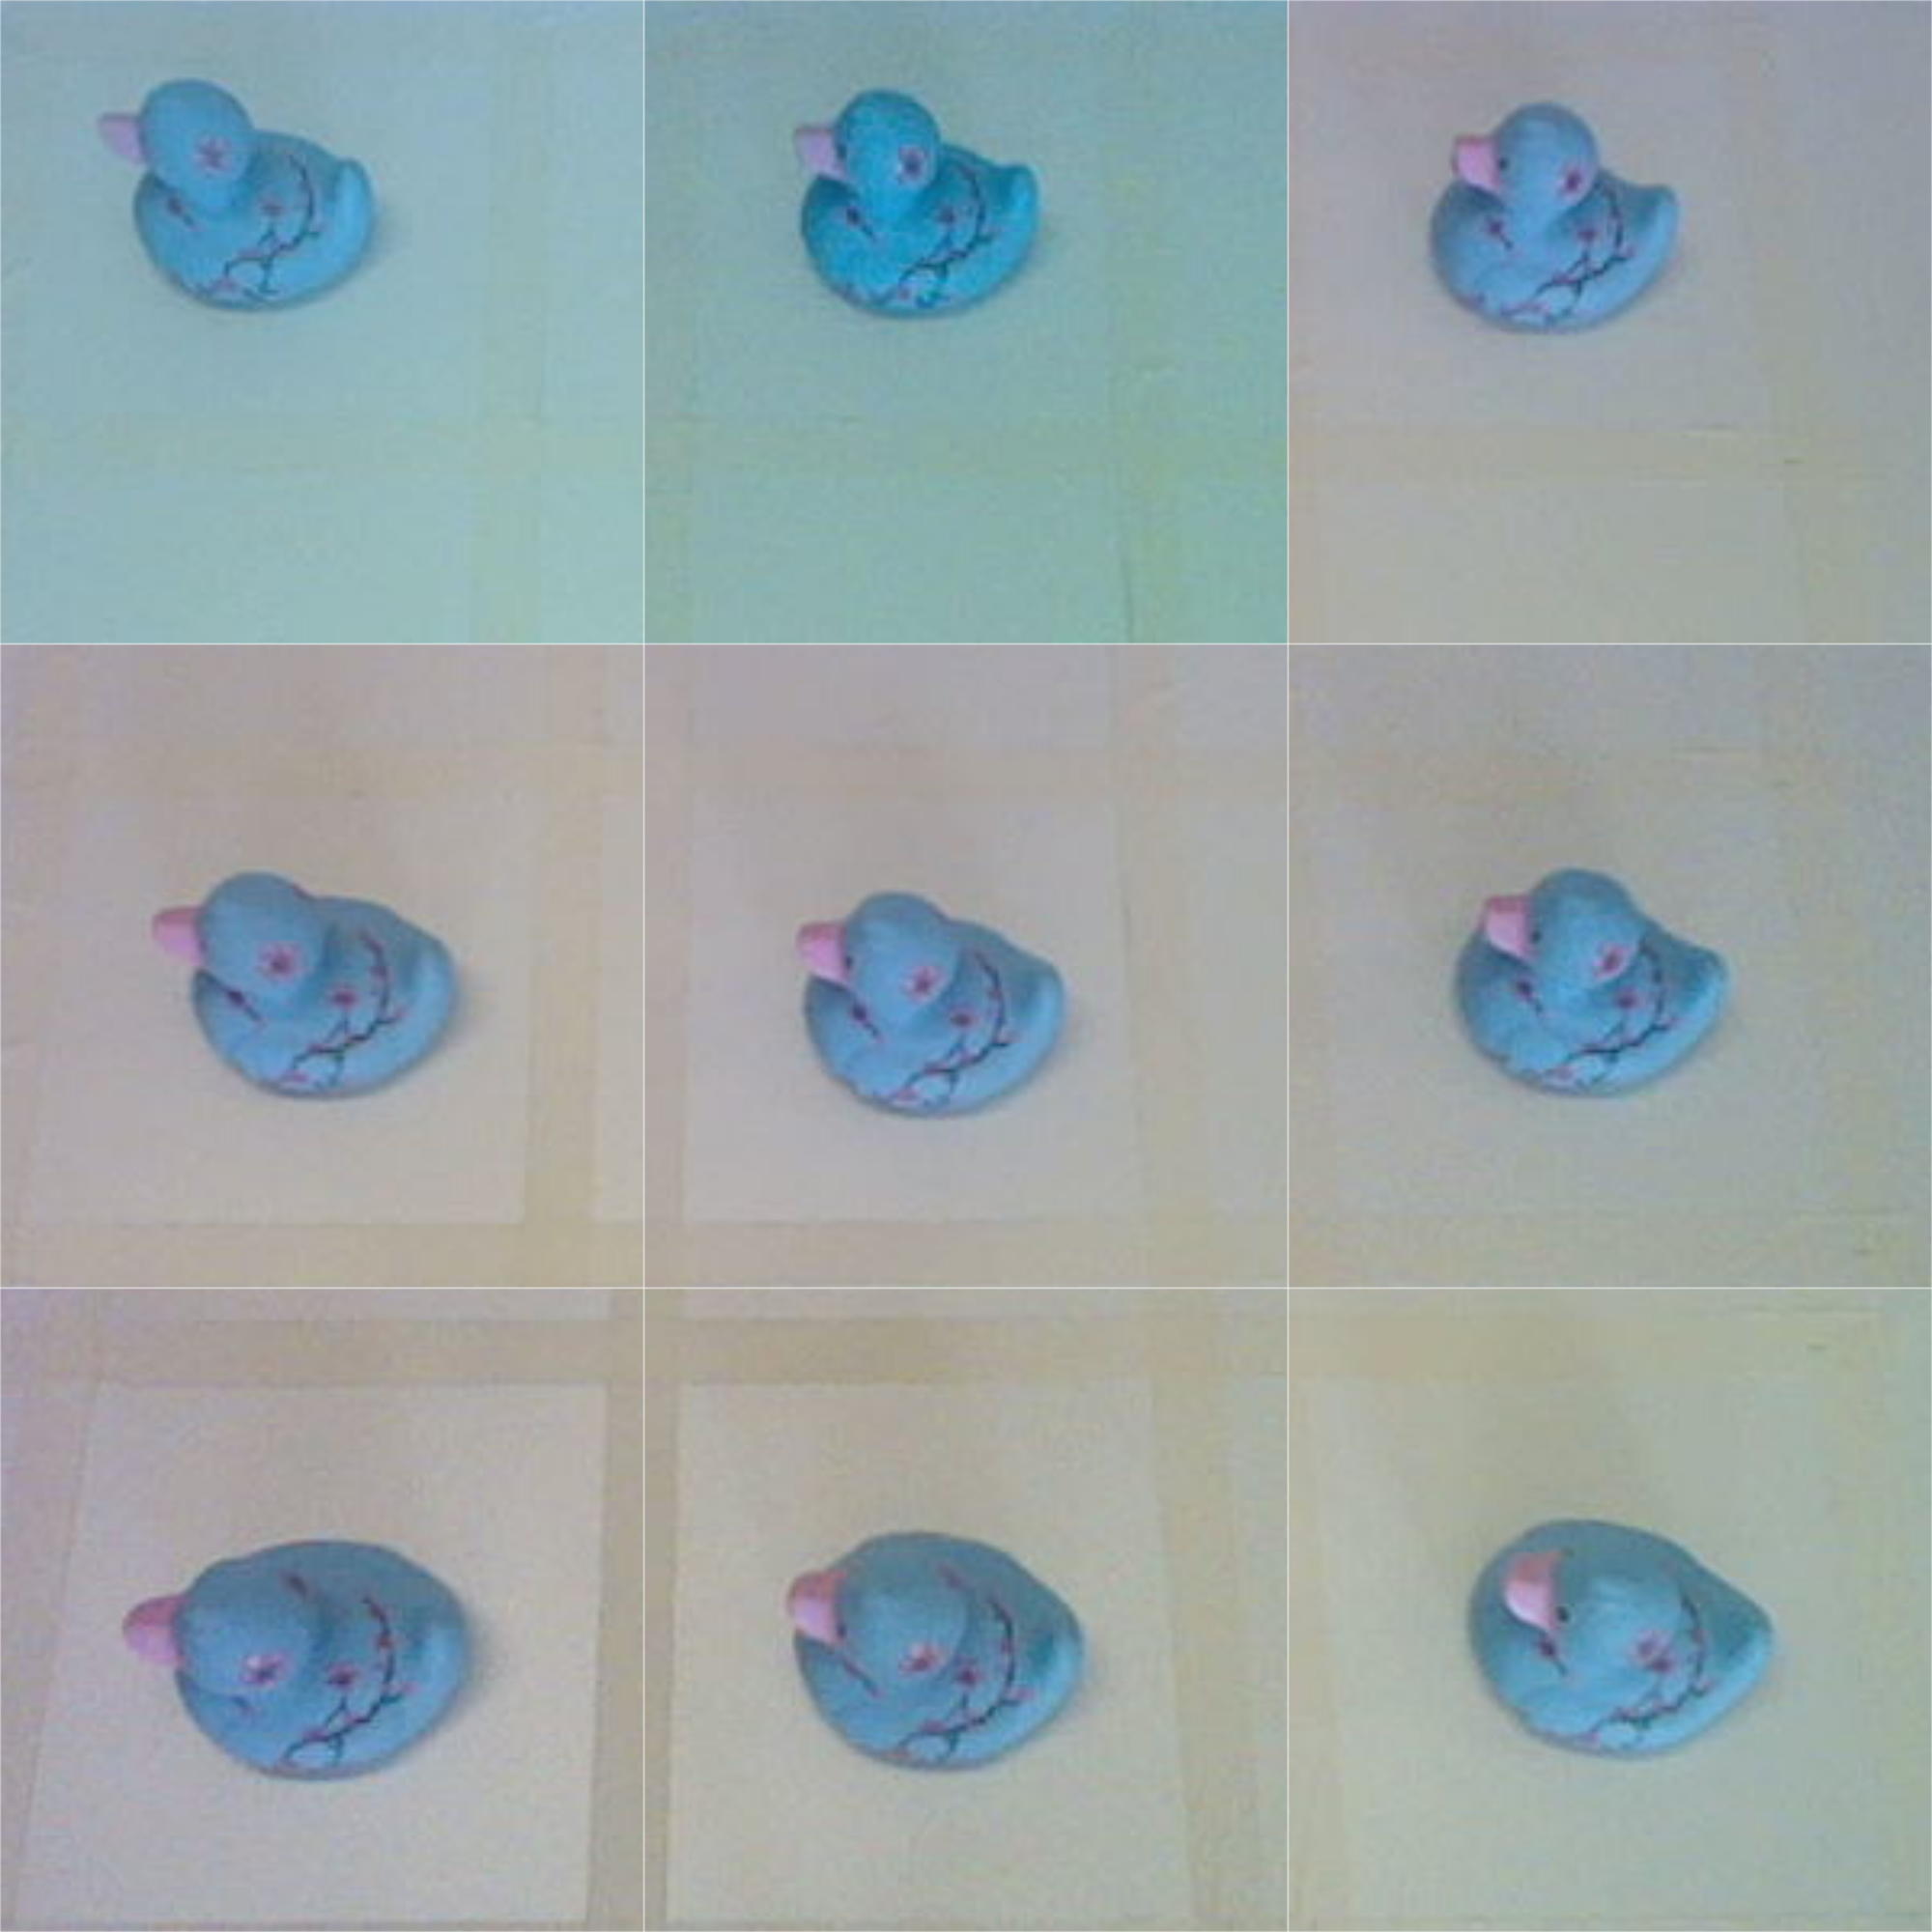
\includegraphics[width=0.7\textwidth]{Figs/chapter6/ReShapeCrop.png}
    \caption{Example cropped images from ReShape.}
    \label{fig:ReShapeCrop}
\end{figure}

Cropping the images is done for three main reasons. 1) this increases the amount of training data for each object by a factor of nine. As the notion of position is removed, the same object in a different position is no longer considered a separate object (unlike in the previous chapter). 2) Cropping reduces the amount of the \ac{MAE}'s field of view which contains the background. This makes it easier for the \ac{MAE} to learn the visual attributes of the objects as less computation is wasted processing the background. 3) Cropping greatly reduces the necessary computation to process a single image as the images are much smaller. Cropping does this without reducing the size of the object in the image unlike resizing the raw image.

Cropping is performed heuristicly, using the position word from the image description to crop out a predefined region. \autoref{fig:CropHeur} shows the regions that each position word relates to for the purposes of cropping.

\begin{figure*}[ht]
    \centering
    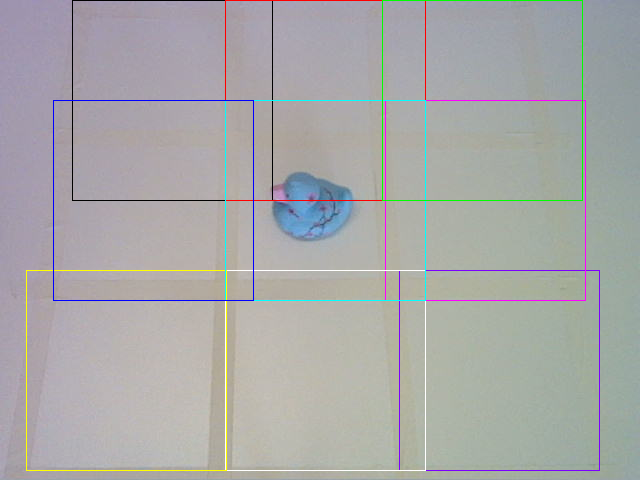
\includegraphics[width=0.7\textwidth]{Figs/chapter6/cropHeuristics.png}
    \caption{Regions to crop to given different postion words.}
    \label{fig:CropHeur}
\end{figure*}


%After cropping, their are changes in the visual attributes of the images which are not accounted for in their descriptions. For example, images in top positions, were further from the camera so they appear slightly smaller than those in bottom positions.

\subsection{Training Procedures}

Calculating the average image for each object provides insight into what to expect when generating images in the Words Only test condition.


\begin{figure*}[ht]
    \centering
    \includegraphics[width=0.7\textwidth]{Figs/chapter6/avgBrickDuckBGY.png}
    \caption{Exp 1: Average of the training images of bricks and ducks in different sizes and colours.}
    \label{fig:AvgBrickDuck}
\end{figure*}

\begin{figure*}[ht]
    \centering
    \includegraphics[width=\textwidth]{Figs/chapter6/avgMost.png}
    \caption{Exp 2: Average of the training images for bricks, cups, donuts, ducks, and rectangles, in different sizes and colours.}
    \label{fig:avgMost}
\end{figure*}

The simple training procedure has the MAE trained to optimise the \ac{MSE} of its output with respect to all of the training data. In the Words Only test condition, the ``best'' images for it to generate are therefore the average images for each object. \autoref{fig:AvgBrickDuck} shows the average image for each object used in experiment 1. \autoref{fig:avgMost} shows the average image for each object in experiment 2.

As the average images are very blurry, it would be useful to have a method which would cause the \ac{MAE} to produce better quality images so that it is easier to inspect which of the visual attributes it has learned to generate correctly.

Using the exemplar training procedure I replace the training image targets with exemplars for each class, when only words are provided as input.

Exemplars are selected by first calculating the average image for each object (\autoref{fig:AvgBrickDuck}, \ref{fig:avgMost}). I then select the training image with the smallest \ac{MSE} from the average image for each object to be the exemplar for that object. 

\autoref{fig:ExmBrickDuck} shows the exemplars used in experiment 1 and \autoref{fig:ExmMost} shows the exemplars for experiment 2.

\begin{figure*}[ht]
    \centering
    \includegraphics[width=0.7\textwidth]{Figs/chapter6/avgBrickDuckBGYExemplars.png}
    \caption{Exp 1: Exemplar images of bricks and ducks in different sizes and colours.}
    \label{fig:ExmBrickDuck}
\end{figure*}


\subsection{Experiment 1}
Experiment 1 makes use of two shapes in three colours and three sizes. The shapes and colours were selected as they are the only shape-colour combinations that occur in all three sizes in the dataset.

\begin{table}[h]
\centering
\begin{tabular}{|c|c|c|}
\hline

\textbf{Shapes}  & \textbf{Colours} & \textbf{Sizes}\\ \hline \hline
Brick  & Yellow  & Big \\ \hline
Duck   & Green   & Medium \\ \hline
& Blue & Small \\ \hline
			  
			
\end{tabular}
\caption{Experiment 1 data subset.}
\label{tab:6_exp1_data} 
\end{table}


\subsubsection{Results}

Overall, the \ac{MAE} has similar performance in terms of \ac{MSE} using both the simple and exemplar training procedures. Whilst the exemplar method lead to slightly better performance in the Bimodal and Image Only test conditions, this is traded off for worse performance in the Words Only condition. The fact that the \ac{MSE} in the Words only condition is small, shows that the mean image for the training and testing data is very similar.

\begin{table}[h!]
\centering
	\begin{tabular}{|c|c|c|c|}
	\hline
\textbf{Training} & 	\textbf{Bimodal} & 	\textbf{Image Only} 	& 	\textbf{Words Only} \\ \hline
Simple & 2.14 $\mypm$ 0.11 & 4.00	$\mypm$ 0.04 & 6.02 $\mypm$ 	0.01 \\ \hline
Exemplar & 2.06 $\mypm$ 0.07 & 3.44 $\mypm$ 0.51 & 7.92	$\mypm$ 0.02 \\ \hline
\end{tabular}
\caption{Exp 1: Total Mean Squared Error for different test conditions and training procedures. (All values are $\times10^{-3}$.)}
\label{tab:6_res_exp1}
\end{table}

The similarity between the training and test data is expected in this case as the dataset was created using the same set of objects, in the same location on the same background. As previously mentioned, the main source of variability in the dataset is caused by changes in lighting conditions across the different data-capture sessions. However, this demonstrates an issue with using \ac{MSE} as the cost function to train the \ac{MAE}. If a different example of an object, captured on a different background, from a different angle is used to test the \ac{MAE}, the \ac{MSE} will be very high in the Words Only condition as this image will be very far from the mean image of the training data.

The addition of more training data, with more diverse examples and more detailed descriptions should help. However, as the system is designed for operation on a robot, its absolute performance on a dataset isn't really that important. It is of more worth that the \ac{MAE} generate a "big blue duck" when asked to, than to generate the specific "big blue duck" the user had in mind.

\paragraph{Image Generation}

Comparing \autoref{fig:simpleGen_1} and \autoref{fig:AvgBrickDuck} it can be seen that the generated images are almost identical to the average training images for each description when the Simple training procedure is used. 

\begin{figure*}[ht]
    \centering
    \includegraphics[width=0.7\textwidth]{Figs/chapter6/avgBrickDuckBGYGenerated.png}
    \caption{Exp 1: Images generated from full descriptions using the \ac{MAE} trained with the simple procedure.}
    \label{fig:simpleGen_1}
\end{figure*}

Similarly, the Exemplar images from \autoref{fig:ExmBrickDuck} and the images generated by the Exemplar \ac{MAE} in \autoref{fig:exemplarGen_1} are also almost identical.

\begin{figure*}[ht]
    \centering
    \includegraphics[width=0.7\textwidth]{Figs/chapter6/avgBrickDuckBGYGeneratedExemplars.png}
    \caption{Exp 1: Images generated from (only) full descriptions using the MAE trained with the exemplar procedure.}
    \label{fig:exemplarGen_1}
\end{figure*}

These two results show that the \ac{MAE} has overfitted the training data, however this isn't necessarily a bad thing as the generated images are correct for the input descriptions and the \ac{MAE} has perfect accuracy at labelling the test data in the Image Only condition (\autoref{tab:6_res_exp1_acc}).



\begin{figure*}[ht]
    \centering
    \includegraphics[width=0.7\textwidth]{Figs/chapter6/2wordsSimpleBrickDuck.png}
    \caption{Exp 1: Images generated using word pairs using the MAE trained with the simple procedure.}
    \label{fig:2wordsSimpleBrickDuck}
\end{figure*}

\begin{figure*}[ht]
    \centering
    \includegraphics[width=0.7\textwidth]{Figs/chapter6/2wordsExemplarBrickDuck.png}
    \caption{Images generated using word pairs using the MAE trained using image exemplars. (Only words are provided as input.)}
    \label{fig:2wordsExemplarBrickDuck}
\end{figure*}


It is hard to tell how well the \ac{MAE} has learnt the grounded meanings of each individual word when the simple training procedure is used as the generated images are very blurry (\autoref{fig:2wordsSimpleBrickDuck}). The meanings of colours and sizes have been correctly learnt with \textsc{Yellow}, \textsc{Green} and  \textsc{Blue} generating the correct coloured pixels. \textsc{Big} \textsc{Medium} and \textsc{Small} also lead to the correct alteration in number of coloured pixels generated.

In \autoref{fig:2wordsExemplarBrickDuck} as well as the correct grounding of the colours and sizes, we also see that the names of the objects have been correctly grounded, with \textsc{brick} generating a square shape and \textsc{Duck} generating a rubber-duck shape. We also see that detials such as the duck's beak are generated as well as the black top hat on the small yellow duck.

Whilst the generation of the beak is desirable, as all ducks have beaks, the top hat is specific to only two instances of ducks in the training data, a \textsc{big yellow duck} and a \textsc{small yellow duck}. The influence of the top hat can be seen in \autoref{fig:simpleGen_1} with the 
\textsc{big yellow duck} having a black area on its head.

The top hat further highlights that the \ac{MAE} learns to generate the mean image for a given object. So, as with the blurring of the images caused by the simple training procedure and remedied by the exemplar procedure, is there a method to reduce the introduction of training data specific artifacts like the top hat?

The simplest method to deal with this, would be to increase the complexity of the descriptions of the images. If the duck with a top hat were referred to as "big yellow duck with a top hat", which could be encoded to the network as \textsc{big yellow duck black top hat} by expanding its vocabulary, then distinguishing whether to generate an image of a duck with or without a top hat would be simple.


\paragraph{Multilabel Classification}

The \ac{MAE} achieves 100\% accuracy on description generation across all three test conditions. This suggests that the test data has a very similar distribution to the training data. As the test data is images of the same objects captured in the same environment, the only differences between the training data and test data will be small changes in object position and  changes in lighting as the test data was captured on a different day and at a different time of day. Thus, the mean image from the training data for each object is likely very close to the mean image for each object in the test data respectively. It is unlikely that such good performance would be achieved with even small changes to viewing angle or background, which are both constant across the training and test data. However, the addition of more diverse training examples would also alleviate this \cite{keller2016analysis, keller}.


\begin{table}[h!]
\centering
	\begin{tabular}{|c|c|c|c|}
	\hline
\textbf{Training }	 & 	\textbf{Bimodal} & \textbf{Image Only} 	& 	\textbf{Words Only} \\ \hline
Simple & 100.00 $\mypm$ 0.00 & 100.00 $\mypm$ 0.00 & 100.00 $\mypm$ 0.00 \\ \hline
Exemplar & 100.00 $\mypm$ 0.00 & 100.00 $\mypm$ 0.00 & 100.00 $\mypm$ 0.00 \\ \hline
	\end{tabular}
\caption{Exp 1: Percentage Description Accuracy for different test conditions and training procedures.}
\label{tab:6_res_exp1_acc}
\end{table}


\subsection{Experiment 2}

Experiment 2 makes use of five shapes in five colours and three sizes. The additional shapes and colours were selected as they are represented in most sizes in the dataset.

\begin{table}[h]
\centering
\begin{tabular}{|c|c|c|}
\hline

\textbf{Shapes}  & \textbf{Colours} & \textbf{Sizes}\\ \hline \hline
Brick  & Yellow  & Big \\ \hline
Duck   & Green   & Medium \\ \hline
Donut & Blue & Small \\ \hline
Cup  & Red & \\ \hline
Rectangle & Black & \\ \hline

\end{tabular}
\caption{Experiment 2 data subset.}
\label{tab:6_exp2_data} 
\end{table}

\begin{figure*}[ht]
    \centering
    \includegraphics[width=\textwidth]{Figs/chapter6/exemplarMost.png}
    \caption{Exp 2: Exemplar images of bricks, cups, donuts, ducks, and rectangles, in different sizes and colours.}
    \label{fig:ExmMost}
\end{figure*}


\subsubsection{Results}

\begin{table}[h!]
\centering
	\begin{tabular}{|c|c|c|c|}
	\hline
\textbf{Training} & 	\textbf{Bimodal} & 	\textbf{Image Only} 	& 	\textbf{Words Only} \\ \hline
Simple &  2.14 $\mypm$	0.07 & 3.89 $\mypm$	0.62 & 6.08 $\mypm$ 0.01 \\ \hline
Exemplar & 2.30 $\mypm$ 0.07 & 3.67 $\mypm$ 0.23
& 10.51	$\mypm$ 0.01 \\ \hline

\end{tabular}
\caption{Exp 2: Total Mean Squared Error for different test conditions and training procedures. (All values are $\times10^{-3}$.)}
\label{tab:6_res_exp2}
\end{table}


\subsubsection{Image Generation}

The \ac{MAE} is able to generalise to unseen combinations of attributes, confirming the result found in the final experiment of the previous chapter (Experiment 5 \autoref{Chapter5}). However, in this case, we have many more missing examples. \autoref{fig:mostExemplarGen} shows the images generated from full descriptions by the \ac{MAE} trained using exemplars. The red borders show images which have exemplars; those without red borders are not seen in the training data, yet the \ac{MAE} is still able to produce good approximations of these objects.

\begin{figure*}[ht]
    \centering
    \includegraphics[width=\textwidth]{Figs/chapter6/exemplarMostGenerated.png}
    \caption{Exp 2: Images generated from full descriptions using the \ac{MAE} trained with the exemplar procedure. Red borders show objects with exemplar images.}
    \label{fig:mostExemplarGen}
\end{figure*}

The clearest example of generalisation to unseen objects is the generation of donuts in \autoref{fig:mostExemplarGen}. Despite only having 3 examples of donuts, the \ac{MAE} is able to generate images of donuts in different colours and sizes.  

The quality of the generated images for unseen objects is strongly linked to whether there is a similar example to the requested image. For example, the \textsc{big green donut} and \textsc{small green donut} are of a higher quality than the \textsc{big red donut} and \textsc{small red donut}. This is due to the existence of a \textsc{medium green donut} in the training data. As there are no red donuts in the training data, the \ac{MAE} must rely on its knowledge of the meanings of the individual words \textsc{big}, \textsc{red} and \textsc{donut} to generate an image of a \textsc{big red donut}. For the \textsc{big green donut}, the \ac{MAE} has an example of a \textsc{medium green donut} so it must only alter the size of the object in the image, it does not need to generate the image from the individual words \textsc{big}, \textsc{green} and \textsc{donut}.

In general the \ac{MAE} shows its worst performance on \textsc{black} objects, this is likely due to the reletively few examples of black objects in the training data (5 for black versus 8 for red, 11 for green, 11 for yellow and 12 for blue).

\textcolor{red}{The correct generation of images of unseen objects demonstrates that the learnt representation has fulfilled at least some of the criteria set out by Bengio et al. \cite{repRev} (hypothesis 5). The fact that the representation of unseen descriptions leads to the generation of correct images shows that the representation has manifolds, in which different symbols reside (e.g. shapes and colors are represented separately, otherwise we would not be able to generate a \textsc{red donut} as the representation of \textsc{red} would be entangled with other words.)}

\begin{figure*}[ht]
    \centering
    \includegraphics[width=\textwidth]{Figs/chapter6/2wordsMostExemplar.png}
    \caption{Exp 2: Images generated using word pairs using the \ac{MAE} trained using image exemplars when only words are provided as input.}
    \label{fig:2wordsMostExemplar}
\end{figure*}


In \autoref{fig:2wordsMostExemplar} we can see the output of the \ac{MAE}'s image output when only two words are given as input. The meaning of the different colours has been learnt with all images in the red (r), yellow, (y) green (g) blue (b) and black (k) rows and columns having their appropriate colour except when two colours are given as input (e.g. "yellow green") which does not have a true meaning in this instance. We do however see that some colours are more dominant than others, (in order, y, g, b, r, k), this is likely due to their prominence in the dataset, with more examples of yellow, green and blue objects than either red or black objects. 

Yellow dominating over blue and green is likely due to less variance in the shade of yellow in the dataset vs the variance in shades of blue and green (similarly for green dominating over blue). This can be seen clearly in \autoref{fig:ExmMost} where nearly all of the yellow objects have the same shade of yellow compared to blue where there is a spectrum of blues from dark to light blue.

The sizes have been correctly learnt with big (B) images having more coloured pixels than medium (M) images which in turn have more coloured pixels than small (S) images.

The different shapes have been learnt to different degrees. For example, the Donut is clearly a ring in all valid cases (i.e. when only one object name is provided as input).

\paragraph{Multilabel Classification}

In \autoref{tab:6_res_exp2} we can see the total \ac{MSE} for generation of images and text in the three different test conditions. In all three condition the \ac{MSE} is very low and has low variance across the four cross validation trials.

\paragraph{Description Accuracy}
\begin{table}[h!]
\centering
	\begin{tabular}{|c|c|c|c|}
	\hline
\textbf{Training}	 & 	\textbf{Bimodal} & \textbf{Image Only} 	& 	\textbf{Words Only} \\ \hline
Simple &  100.00 $\mypm$ 0.00 & 100.00 $\mypm$ 0.00 & 100.00 $\mypm$ 0.00 \\ \hline
Exemplar & 100.00 $\mypm$ 0.00 & 100.00 $\mypm$ 0.00 & 100.00 $\mypm$ 0.00 \\ \hline
\end{tabular}
\caption{Accuracy}
\label{tab:6_res_exp2_acc}
\end{table}


In all three test conditions the \ac{MAE} correctly generates descriptions with 100\% accuracy (\autoref{tab:6_res_exp2_acc}. This is due to the similarity of the training and test data, as previously discussed.

\subsection{Discussion}

Applying \ac{MRL} to real data presents many new challenges as compared to when it is applied to the ArtS dataset. Whilst real images have much more noise in them than artificially generated images, the more important difference between Arts and ReShape is that there are many visual attributes in the ReShape dataset which are not accounted for in the image descriptions.

This showed up as the introduction of image artifacts such as the top hat on the yellow duck in both experiments 1 and 2 as well as the blurring of images generated when class exemplars were not used in training. In the ArtS dataset each object was fully described by its description, whereas in ReShape, there are changes in perspective due to the different locations which images were captured at and visual textures such as patterns on the ducks beyond their primary colour (for example, the duck in \autoref{fig:CropHeur} has a floral pattern but is only described as a \textsc{Big Blue Duck}).

There is also the issue of not having full coverage of every size, colour and shape combination. Whilst \ac{MRL} has been demonstrated to cope well with missing examples, correctly generating images of unseen objects, these images are lower quality than the images generated for objects which have exemplars. The fewer examples of a particular shape, colour or size, the worse the image generation for that attribute. \autoref{fig:mostExemplarGen} highlights this, where \textsc{big black donut} is generated as a \textsc{big brown/yellow donut} as the MAE does not have a strong representation of the colour black and only has three examples of donuts.



\section{Summary}
This chapter focused on how \ac{MRL} could be applied to real data, demonstrating how it can be used to solve the symbol grounding problem in an unsupervised manner.
To that end, I have demonstrated that \ac{MRL} can be used to perform bidirectional grounding of images and text, \textcolor{red}{thus proving hypothesis 6: It is possible to use \ac{MRL} with real data}. Further to this, I have shown that \ac{MRL} can generalise to unseen examples, correctly generating images of unseen objects \textcolor{red}{, and have demonstrated that \ac{MRL} can be useful in a real life scenario}.

The ability of the \ac{MAE} to generate images of unseen objects like the \textsc{Big Red Donut} is very exciting. This result hints at the possibility to develop grounded models capable of understanding more diverse visual attributes and larger numbers of objects.

These experiments present a starting point from which more powerful models can be built through the use of larger datasets as well as through the incorporation of advanced  \ac{ANN} techniques such as dilated and multiscale convolutions, and residual connections. The addition of these types of features to the \ac{MAE} architecture could allow for stronger models of image feature scale and shape and how these relate to the words which describe them.

Further discussion of the results from this chapter has been published in \cite{sheppard2020multimodal}.
\theendnotes 
%% Chapter Template

\chapter{Conclusion} % Main chapter title

\label{Chapter7} % Change X to a consecutive number; for referencing this chapter elsewhere, use \ref{ChapterX}

\lhead{Chapter 7. \emph{Conclusion}} % Change X to a consecutive number; this is for the header on each page - perhaps a shortened title

%----------------------------------------------------------------------------------------
%	SECTION 1
%----------------------------------------------------------------------------------------

\section{Summary of Important Points}
Through the course of the experiments shown in \autoref{Chapter4}, \autoref{Chapter5} and \autoref{Chapter6}, I have demonstrated that  \ac{MRL} can be used to learn a grounded representation of different data modalities in an unsupervised manner.

This representation has been demonstrated to fit the criteria layed out by Bengio et al. in \cite{repRev}. Particularly, the representation has been demonstrated to have Manifolds which can be manipulated through vector arithmetic to make predictable and meaningful changes in the output.

In some datasets, such as MNIST and ArtS, it is possible to generate image prototypes for each class/word in the \ac{MAE}'s ``vocabulary''. For MNIST, this came in the form of prototypical versions of each digit and for ArtS, images of each colour, shape and size can be generated individually.

This is also possible for the ReShape dataset However, due to the larger variability of training examples, the prototypes are very blurry. By using a class exemplar for each object, the \ac{MAE} was able to learn to generate non-blurry prototypes for each of the visual attributes.

I also demonstrated that \ac{MRL} can be used to generate accurate object descriptions of both real and artificial images. As well as that using \ac{MRL} can led to improvements in classification accuracy as seen in \autoref{Chapter4}.

In \autoref{Chapter5} and \autoref{Chapter6} I showed that \ac{MRL} allows \acp{ANN} to generalise to unseen objects. The \ac{MAE} is able to correctly generate images of objects which do not appear in the training data by combining the representations of different words. This entire process relies on the \ac{MAE} having grounded the meaning of each word individually to its image-space equivalent.


\section{Conclusion}
\ac{MRL} has been shown to be a powerful technique and presents an area worthy of futher study. Whilst the findings of the experiments in this thesis are exciting, further work is needed to apply \ac{MRL} in a real world setting.

Unsupervised approaches to symbol grounding are vital to the development of robots for opperation in the real world. \ac{MRL} could form the foundation of a robotic cognitive system which can continue to learn throught its lifetime. Furthermore, the ability of the trained \acp{MAE} to generalise to unseen objects will make teaching robots about new objects quicker as it is not necessary to train the \ac{MAE} with every possible combination of visual attributes. Only a subset of atrribute combinations needs to be learnt, from which other attribute combinations can be inferred as demonstrated in \autoref{Chapter5} when generating images of \textsc{Red Donuts}.


%% Chapter Template

\chapter{Future Work} % Main chapter title

\label{Chapter8} % Change X to a consecutive number; for referencing this chapter elsewhere, use \ref{ChapterX}

\lhead{Chapter 8. \emph{Future Work}} % Change X to a consecutive number; this is for the header on each page - perhaps a shortened title

%----------------------------------------------------------------------------------------
%	SECTION 1
%----------------------------------------------------------------------------------------

\section{What Comes Next?}
The experiments layed out in the previous chapters have shown that \ac{MRL} using \acp{MAE} allows for the unsupervised learning of a grounded representation of images and language. How then, can this be used to improve robotic technologies?

I see many potential applications for \ac{MRL} within the field of \ac{HRI}. \autoref{fig:fsm} shows an example of how the \ac{MAE} can be included in a robotic system.


\begin{figure}
\centering
\includegraphics[width=\textwidth]{Figs/futureWork/fsm.png}
\caption{An example of how the \ac{MAE} can be used as part of a robotic system.}
\label{fig:fsm}
\end{figure}

Consider the scenario of a human interacting with a robot to teach it a set of objects and their visual attributes as well as the words used to describe the objects and their visual attributes. In a laboratory setting it is feasable to have only a single object in view at any given time. This is not true for real world scenarios. However, with the introduction of a \ac{FSM} controlled via a \ac{NLU} module, it is simple to use a \ac{MAE} trained with \ac{MRL} to discern which object is being referred to by the human. This is demonstrated in \autoref{fig:disamb}

\begin{figure}
\centering
\includegraphics[width=\textwidth]{Figs/shapes/findingRefferant.png}
\caption{An example of using an MAE trained with MRL to disambiguate which object is being referred to in a scene.}
\label{fig:disamb}
\end{figure}

First, the image is split into patches, this can be done naively by sliding a window over the image and processing each patch. However this is not very computationally efficient and is likely to give ambiguous results, depending on the stride of the window, as multiple image patches may contain parts of the object of interest. Therefore it would be sensible to make use of an object detector such as Yolo v3 \cite{redmon2018yolov3} to predict object bounding boxes.

Comparing the embedding of each image patch to the embedding of the query, the image patch of interest should have the smallest \ac{MSE} between it and the query.

In order for the scenario depicted in \ref{fig:disamb}, an \ac{NLU} module must be trained to extract the Intent of the human's utterance as well as any Entities which the human refers to. Fortunately, these types of \acp{NLU} are easily built using open source libraries like Rasa \cite{rasa}.



Developing the infrastructure for this type of scenario would allow for the exploration of questions such as:

\begin{itemize}
\item How many training examples does the \ac{MAE} require to operate accurately?
\item Is their an upper limit on the number of objects, visual attributes and words which the \ac{MAE} can learn?
\item How does regenerating a missing modality affect classification accuracy? Can the embedding of the regnerated missing modality be exploited to enhance  multimodal recognition techniques?
\end{itemize}

I believe \ac{MRL} can be used as a general tool for facilitating \ac{HRI} experiments, with the \ac{MAE} providing a piece of a cognitive architecture which translates low level sensory percepts (vision) to high level symbols (language).


%-----------------------------------
%	SUBSECTION 1
%-----------------------------------
 

%----------------------------------------------------------------------------------------
%	THESIS CONTENT - APPENDICES
%----------------------------------------------------------------------------------------

\addtocontents{toc}{\vspace{2em}} % Add a gap in the Contents, for aesthetics

\appendix % Cue to tell LaTeX that the following 'chapters' are Appendices

% Include the appendices of the thesis as separate files from the Appendices folder
% Uncomment the lines as you write the Appendices

%% Appendix A

\chapter{Publications} % Main appendix title

\label{AppendixA} % For referencing this appendix elsewhere, use \ref{AppendixA}

\lhead{Appendix A. \emph{Publications}} % This is for the header on each page - perhaps a shortened title
\label{app:A}
\begin{itemize}
	\item E. Sheppard, H. Lehmann, G. Rajendran, P. E. McKenna, O Lemon , K. S. Lohan, Towards Better Human Robot Interaction:
Multimodal Learning of MNIST Handwritten Digits. - Submitted to ICDL - epirob 2018
	\item K. S. Lohan, E. Sheppard, G. E. Little, G. Rajendran (2016), Distinguishing children with ASD using pupil diameter metrics. 6th Joint IEEE International Conferenceon on Development and Learning and on Epigenetic Robotics 2016
    \item{E.Sheppard, K. S. Lohan,G.E. Little , L. Bonnar , S. Kelly and G. Rajendran, (2017) Understanding the difference in pupil dilation between children with and
without ASD during a joint attention memory task, 3rd Workshop on Child-Robot Interaction at Human-Robot Interaction 2017}
	\item{E. Sheppard, K. S. Lohan,G.E. Little, G. Rajendran (2018) Towards improved child robot interaction by
understanding eye movements,IEEE TCDS Special Issue A sense of interaction in humans and robots: from visual perception to social cognition 2018}
\end{itemize}


%\includepdf[pages={1-6},width=\textwidth]{Chapters/icdl2018.pdf}

%\includepdf[pages={1-5},width=\textwidth]{Chapters/LohanAAAI.pdf}

%\includepdf[pages={1-4},width=\textwidth]{Chapters/Lohanetal.pdf}

%\includepdf[pages={1-10},width=\textwidth]{Chapters/ASDTD.pdf}




%\chapter{Appendix \emph{Magical Vectors and where to find them}}
\label{appendix:B}
\lhead{Appendix \emph{Magical Vectors and where to find them}}

This is the appendix for \autoref{Chapter5}.

\begin{table}
		\centering
		\begin{tabular}{|c|c|c|c|c|c|c|}
			\hline
			Block & Layer & Type & Neurons & Kernel & Strides & Activation \\ \hline
			\multirow{3}{*}{Image} & 1i	&	2D Conv & 64 & (3,3) & (1,1) & Relu \\ \cline{2-7}
			& 2i	&	2D Conv & 64 & (3,3) & (2,2) & Relu \\ \cline{2-7}
			& 3i	&	2D Conv & 32 & (3,3) & (2,2) & Relu \\ \cline{2-7}
\multirow{3}{*}{Encoder} & 4i	&	2D Conv & 32 & (3,3) & (2,2) & Relu \\ \cline{2-7}
			& 5i	&	2D Conv & 16 & (3,3) & (2,2) & Relu \\ \cline{2-7}
			& 6i	&	2D Conv & 16 & (3,3) & (2,2) & Relu \\ \cline{2-7}
			& 7i	&	Dropout p=0.25 &	 & 	     &       &  \\ \hline

			\multirow{3}{*}{Word} & 1w	& Dense & 128 & & &TanH \\ \cline{2-7}
			& 2w	& Dense & 256 & & &TanH \\ \cline{2-7}
			& 3w 	&	Dropout p=0.5 &	 & 	     &       & \\ \cline{2-7}
\multirow{4}{*}{Encoder}& 4w  &	Reshape (16,16,1) & & & & \\ \cline{2-7}
			& 5w	&	2D Conv & 16 & (3,3) & (2,2) & Relu \\ \cline{2-7}
			& 6w	&	2D Conv & 16 & (3,3) & (2,2) & Relu \\ \cline{2-7}
			& 7w	&	2D Conv & 16 & (3,3) & (2,2) & Relu \\ \hline

			Merge & 8iw	& Merge & & & & \\ \hline
Embedding & 9iw	&	2D Conv  & emb size & (3,3) & (1,1) & Relu \\ \hline
			
			
			\multirow{4}{*}{Image} & 10i 	&	Dropout p=0.25 &	 & 	     &       & \\ \cline{2-7}
			& 11i	&	2D Trans Conv & 16 & (3,3) & (2,2)  & TanH \\ \cline{2-7}
			& 12i	&	2D Trans Conv & 16 & (3,3) & (2,2)  & TanH \\ \cline{2-7}
			& 13i	&	2D Trans Conv & 16 & (3,3) & (2,2)  & TanH \\ \cline{2-7}
\multirow{4}{*}{Decoder}& 14i	&	2D Trans Conv & 32 & (3,3) & (1,1)  & TanH \\ \cline{2-7}
			& 15i	&	2D Trans Conv & 64 & (3,3) & (1,1)  & TanH \\ \cline{2-7}
			& 16i	&	2D Trans Conv & 64 & (3,3) & (1,1)  & TanH \\ \cline{2-7}
			& 17i	&	2D Trans Conv & 3 & (3,3) & (1,1) & Sigmoid\\ \hline 

			\multirow{4}{*}{Word} & 10w 	&	Dropout p=0.25 &	 & 	     &       & \\ \cline{2-7}
			& 12w	&	2D Trans Conv & 16 & (3,3) & (2,2)  & Relu \\ \cline{2-7}
			& 13w	&	2D Trans Conv & 16 & (3,3) & (2,2)  & Relu \\ \cline{2-7}
			& 14w	&	2D Trans Conv & 16 & (3,3) & (2,2)  & Relu \\ \cline{2-7}
\multirow{5}{*}{Decoder}& 15w	& Reshape (256) & & & & \\ \cline{2-7}
			& 16w	& Dropout p=0.5 &	 & 	     &       & \\ \cline{2-7}
			& 17w	& Dense & 256 & & &TanH \\ \cline{2-7}
			& 18w	& Dense & 128 & & &TanH \\ \cline{2-7}
			& 19w	& Dense & 22 & & & Sigmoid \\ \hline
			
			
		\end{tabular}
		\caption{Image and Word multimodal autoencoder. Layers marked i, w, and iw are image, word, and image and word respectively. The number of neurons, ``emb size'', in the Embedding block is varied in some experiments.}
		\label{tab:Arts_MAE_description}

	\end{table}
%This appendix contains extra figures from \autoref{Chapter5}
%\begin{figure}
%\centering
%\includegraphics[width=0.75\textwidth]{Figs/shapes/singlelabel331A.png}
%\caption{Images generated of each word for different sizes of embedding using the MAE trained in experiment 1 run A.}
%\label{fig:331singleA}
%\end{figure}
%\begin{figure}
%\centering
%\includegraphics[width=0.75\textwidth]{Figs/shapes/singlelabel331B.png}
%\caption{Images generated of each word for different sizes of embedding using the MAE trained in experiment 1 run B.}
%\label{fig:331singleB}
%\end{figure}
%\begin{figure}
%\centering
%\includegraphics[width=0.75\textwidth]{Figs/shapes/singlelabel331C.png}
%\caption{Images generated of each word for different sizes of embedding using the MAE trained in experiment 1 run C.}
%\label{fig:331singleC}
%\end{figure}
%\begin{figure}
%\centering
%\includegraphics[width=0.75\textwidth]{Figs/shapes/singlelabel331D.png}
%\caption{Images generated of each word for different sizes of embedding using the MAE trained in experiment 1 run D.}
%\label{fig:331singleD}
%\end{figure}


\begin{figure}
\centering
\includegraphics[width=0.75\textwidth]{Figs/shapes/331_8v200.png}
\caption{Images generated from descriptions with an embedding size of 8 or 200.}
\label{fig:8vs200}
\end{figure}

The number of weight updates during training is given by \autoref{eqn:updates}.

\begin{equation}\label{eqn:updates}
u = E \times S \times Obj \times C \times Sz \times pos
\end{equation}

Where $u$ is th number of updates, $E$ the number of epochs of training, $S$ the number of samples for each shape, colour, size, position combination, $Obj$ the number of shapes, $C$ the number of colours, $Sz$ the number of sizes and $pos$ the number of positions.


\begin{table}
\centering
\begin{tabular}{|c|c|c|c|c|c|c|c|}
\hline
Experiment & Samples & Shapes & Colours & Sizes & Positions & Updates per Epoch \\ \hline
Exp 1 & 50 & 3 & 3 & 1 & 3 & 1350 \\ \hline
Exp 2 & 50 & 3 & 3 & 3 & 3 & 4050 \\ \hline
Exp 3 & 50 & 3 & 3 & 3 & 9 & 12150 \\ \hline
Exp 4 & 50 & 3 & 7 & 3 & 9 & 28350 \\ \hline

\end{tabular}
\caption{Number of weight updates per Epoch for each experiment.}
\label{tab:updatesperEpoch}
\end{table}

\autoref{tab:updatesperEpoch} shows how many times per epoch the weights of the MAE are updated in each experiment. As more data is available in later experiments due to the increase in number of shape-colour-size-position combinations, there are more weight updates per epoch. 

The total number of weight updates a MAE recieves therefore depends on the data it is trained on. Whilst all MAEs in experiment 3 are trained for a total of 100 epochs, for the MAEs which are pretrained, 50 of these epochs are with less data than the full amount available in experiment 3.


%\begin{figure}
%\centering
%\includegraphics[width=0.75\textwidth]{Figs/shapes/singlelabel333A.png}
%\caption{Images generated of each word for different sizes of embedding using the MAE trained in experiment 2 run A.}
%\label{fig:333singleA}
%\end{figure}
%\begin{figure}
%\centering
%\includegraphics[width=0.75\textwidth]{Figs/shapes/singlelabel333B.png}
%\caption{Images generated of each word for different sizes of embedding using the MAE trained in experiment 2 run B.}
%\label{fig:333singleB}
%\end{figure}
%\begin{figure}
%\centering
%\includegraphics[width=0.75\textwidth]{Figs/shapes/singlelabel333C.png}
%\caption{Images generated of each word for different sizes of embedding using the MAE trained in experiment 2 run C.}
%\label{fig:333singleC}
%\end{figure}
%\begin{figure}
%\centering
%\includegraphics[width=0.75\textwidth]{Figs/shapes/singlelabel333D.png}
%\caption{Images generated of each word for different sizes of embedding using the MAE trained in experiment 2 run D.}
%\label{fig:333singleD}
%\end{figure}
%
%\begin{figure}
%\centering
%\includegraphics[width=0.75\textwidth]{Figs/shapes/2word333A.png}
%\caption{Images generated using word pairs using an embedding size of 296 neurons from experiment 2 run A.}
%\label{fig:2word333A}
%\end{figure}
%
%\begin{figure}
%\centering
%\includegraphics[width=0.75\textwidth]{Figs/shapes/2word333B.png}
%\caption{Images generated using word pairs using an embedding size of 296 neurons from experiment 2 run B.}
%\label{fig:2word333B}
%\end{figure}
%
%\begin{figure}
%\centering
%\includegraphics[width=0.75\textwidth]{Figs/shapes/2word333C.png}
%\caption{Images generated using word pairs using an embedding size of 296 neurons from experiment 2 run C.}
%\label{fig:2word333C}
%\end{figure}
%
%\begin{figure}
%\centering
%\includegraphics[width=0.75\textwidth]{Figs/shapes/2word333D.png}
%\caption{Images generated using word pairs using an embedding size of 296 neurons from experiment 2 run D.}
%\label{fig:2word333D}
%\end{figure}
%
%
%
%\begin{figure}
%\centering
%\includegraphics[width=\textwidth]{Figs/shapes/2word339A.png}
%\caption{Images generated using word pairs using a MAE initialised with random weights for experiment 3 run A.}
%\label{fig:2word339A}
%\end{figure}
%
%\begin{figure}
%\centering
%\includegraphics[width=\textwidth]{Figs/shapes/2word339B.png}
%\caption{Images generated using word pairs using a MAE initialised with random weights for experiment 3 run B.}
%\label{fig:2word339B}
%\end{figure}
%
%\begin{figure}
%\centering
%\includegraphics[width=\textwidth]{Figs/shapes/2word339C.png}
%\caption{Images generated using word pairs using a MAE initialised with random weights for experiment 3 run C.}
%\label{fig:2word339C}
%\end{figure}
%
%\begin{figure}
%\centering
%\includegraphics[width=\textwidth]{Figs/shapes/2word339D.png}
%\caption{Images generated using word pairs using a MAE initialised with random weights for experiment 3 run D.}
%\label{fig:2word339D}
%\end{figure}
%
%\begin{figure}
%\centering
%\includegraphics[width=\textwidth]{Figs/shapes/2word339A1.png}
%\caption{Images generated using word pairs using a MAE initialised with weights from experiment 1 for experiment 3 run A.}
%\label{fig:2word339A1}
%\end{figure}
%
%\begin{figure}
%\centering
%\includegraphics[width=\textwidth]{Figs/shapes/2word339B1.png}
%\caption{Images generated using word pairs using a MAE initialised with weights from experiment 1 forexperiment 3 run B.}
%\label{fig:2word339B1}
%\end{figure}
%
%\begin{figure}
%\centering
%\includegraphics[width=\textwidth]{Figs/shapes/2word339C1.png}
%\caption{Images generated using word pairs using a MAE initialised with weights from experiment 1 for experiment 3 run C.}
%\label{fig:2word339C1}
%\end{figure}
%
%\begin{figure}
%\centering
%\includegraphics[width=\textwidth]{Figs/shapes/2word339D1.png}
%\caption{Images generated using word pairs using a MAE initialised with weights from experiment 1 for experiment 3 run D.}
%\label{fig:2word339D1}
%\end{figure}
%
%\begin{figure}
%\centering
%\includegraphics[width=\textwidth]{Figs/shapes/2word339A2.png}
%\caption{Images generated using word pairs using a MAE initialised with weights from experiment 2 for experiment 3 run A.}
%\label{fig:2word339A2}
%\end{figure}
%
%\begin{figure}
%\centering
%\includegraphics[width=\textwidth]{Figs/shapes/2word339B2.png}
%\caption{Images generated using word pairs using a MAE initialised with weights from experiment 2 forexperiment 3 run B.}
%\label{fig:2word339B2}
%\end{figure}
%
%\begin{figure}
%\centering
%\includegraphics[width=\textwidth]{Figs/shapes/2word339C2.png}
%\caption{Images generated using word pairs using a MAE initialised with weights from experiment 2 for experiment 3 run C.}
%\label{fig:2word339C2}
%\end{figure}
%
%\begin{figure}
%\centering
%\includegraphics[width=\textwidth]{Figs/shapes/2word339D2.png}
%\caption{Images generated using word pairs using a MAE initialised with weights from experiment 2 for experiment 3 run D.}
%\label{fig:2word339D2}
%\end{figure}
%
%
%
%
%\begin{figure}
%\centering
%\includegraphics[width=\textwidth]{Figs/shapes/2word739A.png}
%\caption{Images generated using word pairs using a MAE initialised with random weights for experiment 4 run A.}
%\label{fig:2word739A}
%\end{figure}
%
%\begin{figure}
%\centering
%\includegraphics[width=\textwidth]{Figs/shapes/2word739B.png}
%\caption{Images generated using word pairs using a MAE initialised with random weights for experiment 4 run B.}
%\label{fig:2word739B}
%\end{figure}
%
%\begin{figure}
%\centering
%\includegraphics[width=\textwidth]{Figs/shapes/2word739C.png}
%\caption{Images generated using word pairs using a MAE initialised with random weights for experiment 4 run C.}
%\label{fig:2word739C}
%\end{figure}
%
%\begin{figure}
%\centering
%\includegraphics[width=\textwidth]{Figs/shapes/2word739D.png}
%\caption{Images generated using word pairs using a MAE initialised with random weights for experiment 4 run D.}
%\label{fig:2word739D}
%\end{figure}
%
%
%\begin{figure}
%\centering
%\includegraphics[width=\textwidth]{Figs/shapes/2word739A1.png}
%\caption{Images generated using word pairs using a MAE initialised with weights from experiment 1 for experiment 4 run A.}
%\label{fig:2word739A1}
%\end{figure}
%
%\begin{figure}
%\centering
%\includegraphics[width=\textwidth]{Figs/shapes/2word739B1.png}
%\caption{Images generated using word pairs using a MAE initialised with weights from experiment 1 for experiment 4 run B.}
%\label{fig:2word739B1}
%\end{figure}
%
%\begin{figure}
%\centering
%\includegraphics[width=\textwidth]{Figs/shapes/2word739C1.png}
%\caption{Images generated using word pairs using a MAE initialised with weights from experiment 1 for experiment 4 run C.}
%\label{fig:2word739C1}
%\end{figure}
%
%\begin{figure}
%\centering
%\includegraphics[width=\textwidth]{Figs/shapes/2word739D1.png}
%\caption{Images generated using word pairs using a MAE initialised with weights from experiment 1 for experiment 4 run D.}
%\label{fig:2word739D1}
%\end{figure}
%
%\begin{figure}
%\centering
%\includegraphics[width=\textwidth]{Figs/shapes/2word739A2.png}
%\caption{Images generated using word pairs using a MAE initialised with weights from experiment 2 for experiment 4 run A.}
%\label{fig:2word739A2}
%\end{figure}
%
%\begin{figure}
%\centering
%\includegraphics[width=\textwidth]{Figs/shapes/2word739B2.png}
%\caption{Images generated using word pairs using a MAE initialised with weights from experiment 2 for experiment 4 run B.}
%\label{fig:2word739B2}
%\end{figure}
%
%\begin{figure}
%\centering
%\includegraphics[width=\textwidth]{Figs/shapes/2word739C2.png}
%\caption{Images generated using word pairs using a MAE initialised with weights from experiment 2 for experiment 4 run C.}
%\label{fig:2word739C2}
%\end{figure}
%
%\begin{figure}
%\centering
%\includegraphics[width=\textwidth]{Figs/shapes/2word739D2.png}
%\caption{Images generated using word pairs using a MAE initialised with weights from experiment 2 for experiment 4 run D.}
%\label{fig:2word739D2}
%\end{figure}
%
%
%\begin{figure}
%\centering
%\includegraphics[width=\textwidth]{Figs/shapes/2word739A3.png}
%\caption{Images generated using word pairs using a MAE initialised with weights from experiment 3 for experiment 4 run A.}
%\label{fig:2word739A3}
%\end{figure}
%
%\begin{figure}
%\centering
%\includegraphics[width=\textwidth]{Figs/shapes/2word739B3.png}
%\caption{Images generated using word pairs using a MAE initialised with weights from experiment 3 for experiment 4 run B.}
%\label{fig:2word739B3}
%\end{figure}
%
%\begin{figure}
%\centering
%\includegraphics[width=\textwidth]{Figs/shapes/2word739C3.png}
%\caption{Images generated using word pairs using a MAE initialised with weights from experiment 3 for experiment 4 run C.}
%\label{fig:2word739C3}
%\end{figure}
%
%\begin{figure}
%\centering
%\includegraphics[width=\textwidth]{Figs/shapes/2word739D3.png}
%\caption{Images generated using word pairs using a MAE initialised with weights from experiment 3 for experiment 4 run D.}
%\label{fig:2word739D3}
%\end{figure}
%
%
%\begin{figure}
%\centering
%\includegraphics[width=\textwidth]{Figs/shapes/2word739A31.png}
%\caption{Images generated using word pairs using a MAE initialised with weights from experiment 1 + 3 for experiment 4 run A.}
%\label{fig:2word739A31}
%\end{figure}
%
%\begin{figure}
%\centering
%\includegraphics[width=\textwidth]{Figs/shapes/2word739B31.png}
%\caption{Images generated using word pairs using a MAE initialised with weights from experiment 1 + 3 for experiment 4 run B.}
%\label{fig:2word739B31}
%\end{figure}
%
%\begin{figure}
%\centering
%\includegraphics[width=\textwidth]{Figs/shapes/2word739C31.png}
%\caption{Images generated using word pairs using a MAE initialised with weights from experiment 1 + 3 for experiment 4 run C.}
%\label{fig:2word739C31}
%\end{figure}
%
%\begin{figure}
%\centering
%\includegraphics[width=\textwidth]{Figs/shapes/2word739D31.png}
%\caption{Images generated using word pairs using a MAE initialised with weights from experiment 1 for experiment 4 run D.}
%\label{fig:2word739D31}
%\end{figure}
%
%
%
%
%
%\begin{figure}
%\centering
%\includegraphics[width=\textwidth]{Figs/shapes/2word739A32.png}
%\caption{Images generated using word pairs using a MAE initialised with weights from experiment 2 + 3 for experiment 4 run A.}
%\label{fig:2word739A32}
%\end{figure}
%
%\begin{figure}
%\centering
%\includegraphics[width=\textwidth]{Figs/shapes/2word739B32.png}
%\caption{Images generated using word pairs using a MAE initialised with weights from experiment 2 + 3 for experiment 4 run B.}
%\label{fig:2word739B32}
%\end{figure}
%
%\begin{figure}
%\centering
%\includegraphics[width=\textwidth]{Figs/shapes/2word739C32.png}
%\caption{Images generated using word pairs using a MAE initialised with weights from experiment 2 + 3 for experiment 4 run C.}
%\label{fig:2word739C32}
%\end{figure}
%
%\begin{figure}
%\centering
%\includegraphics[width=\textwidth]{Figs/shapes/2word739D32.png}
%\caption{Images generated using word pairs using a MAE initialised with weights from experiment 2 for experiment 4 run D.}
%\label{fig:2word739D32}
%\end{figure}




%\input{Appendices/AppendixC}

\addtocontents{toc}{\vspace{2em}} % Add a gap in the Contents, for aesthetics

\backmatter

%----------------------------------------------------------------------------------------
%	BIBLIOGRAPHY
%----------------------------------------------------------------------------------------

\label{Bibliography}

\lhead{\emph{Bibliography}} % Change the page header to say "Bibliography"

\bibliographystyle{apalike} % Use the "apalike" BibTeX style for formatting the Bibliography

\bibliography{Bibliography} % The references (bibliography) information are stored in the file named "Bibliography.bib"

\end{document}